\documentclass[twoside]{book}

% Packages required by doxygen
\usepackage{fixltx2e}
\usepackage{calc}
\usepackage{doxygen}
\usepackage[export]{adjustbox} % also loads graphicx
\usepackage{graphicx}
\usepackage[utf8]{inputenc}
\usepackage{makeidx}
\usepackage{multicol}
\usepackage{multirow}
\PassOptionsToPackage{warn}{textcomp}
\usepackage{textcomp}
\usepackage[nointegrals]{wasysym}
\usepackage[table]{xcolor}

% Font selection
\usepackage[T1]{fontenc}
\usepackage[scaled=.90]{helvet}
\usepackage{courier}
\usepackage{amssymb}
\usepackage{sectsty}
\renewcommand{\familydefault}{\sfdefault}
\allsectionsfont{%
  \fontseries{bc}\selectfont%
  \color{darkgray}%
}
\renewcommand{\DoxyLabelFont}{%
  \fontseries{bc}\selectfont%
  \color{darkgray}%
}
\newcommand{\+}{\discretionary{\mbox{\scriptsize$\hookleftarrow$}}{}{}}

% Page & text layout
\usepackage{geometry}
\geometry{%
  a4paper,%
  top=2.5cm,%
  bottom=2.5cm,%
  left=2.5cm,%
  right=2.5cm%
}
\tolerance=750
\hfuzz=15pt
\hbadness=750
\setlength{\emergencystretch}{15pt}
\setlength{\parindent}{0cm}
\setlength{\parskip}{3ex plus 2ex minus 2ex}
\makeatletter
\renewcommand{\paragraph}{%
  \@startsection{paragraph}{4}{0ex}{-1.0ex}{1.0ex}{%
    \normalfont\normalsize\bfseries\SS@parafont%
  }%
}
\renewcommand{\subparagraph}{%
  \@startsection{subparagraph}{5}{0ex}{-1.0ex}{1.0ex}{%
    \normalfont\normalsize\bfseries\SS@subparafont%
  }%
}
\makeatother

% Headers & footers
\usepackage{fancyhdr}
\pagestyle{fancyplain}
\fancyhead[LE]{\fancyplain{}{\bfseries\thepage}}
\fancyhead[CE]{\fancyplain{}{}}
\fancyhead[RE]{\fancyplain{}{\bfseries\leftmark}}
\fancyhead[LO]{\fancyplain{}{\bfseries\rightmark}}
\fancyhead[CO]{\fancyplain{}{}}
\fancyhead[RO]{\fancyplain{}{\bfseries\thepage}}
\fancyfoot[LE]{\fancyplain{}{}}
\fancyfoot[CE]{\fancyplain{}{}}
\fancyfoot[RE]{\fancyplain{}{\bfseries\scriptsize Generated by Doxygen }}
\fancyfoot[LO]{\fancyplain{}{\bfseries\scriptsize Generated by Doxygen }}
\fancyfoot[CO]{\fancyplain{}{}}
\fancyfoot[RO]{\fancyplain{}{}}
\renewcommand{\footrulewidth}{0.4pt}
\renewcommand{\chaptermark}[1]{%
  \markboth{#1}{}%
}
\renewcommand{\sectionmark}[1]{%
  \markright{\thesection\ #1}%
}

% Indices & bibliography
\usepackage{natbib}
\usepackage[titles]{tocloft}
\setcounter{tocdepth}{3}
\setcounter{secnumdepth}{5}
\makeindex

% Hyperlinks (required, but should be loaded last)
\usepackage{ifpdf}
\ifpdf
  \usepackage[pdftex,pagebackref=true]{hyperref}
\else
  \usepackage[ps2pdf,pagebackref=true]{hyperref}
\fi
\hypersetup{%
  colorlinks=true,%
  linkcolor=blue,%
  citecolor=blue,%
  unicode%
}

% Custom commands
\newcommand{\clearemptydoublepage}{%
  \newpage{\pagestyle{empty}\cleardoublepage}%
}

\usepackage{caption}
\captionsetup{labelsep=space,justification=centering,font={bf},singlelinecheck=off,skip=4pt,position=top}

%===== C O N T E N T S =====

\begin{document}

% Titlepage & ToC
\hypersetup{pageanchor=false,
             bookmarksnumbered=true,
             pdfencoding=unicode
            }
\pagenumbering{roman}
\begin{titlepage}
\vspace*{7cm}
\begin{center}%
{\Large D\+B\+L\+P-\/\+A\+P-\/\+Project }\\
\vspace*{1cm}
{\large Generated by Doxygen 1.8.11}\\
\end{center}
\end{titlepage}
\clearemptydoublepage
\tableofcontents
\clearemptydoublepage
\pagenumbering{arabic}
\hypersetup{pageanchor=true}

%--- Begin generated contents ---
\chapter{About Repo}
\label{md_README}
\hypertarget{md_README}{}
This repo was created to collaborate for Advanced Programming(C\+SE 201 @ I\+I\+I\+T-\/D) Project

\subsection*{About Project}

Objective is to create a D\+B\+LP Query Engine that parses data from the given X\+ML file.

\subsection*{Contributors}


\begin{DoxyItemize}
\item \href{https://github.com/aklife97}{\tt Abhinav Khattar}
\item \href{https://github.com/tushar1208}{\tt Tushar Arora}
\end{DoxyItemize}

\subsection*{Resources}

The X\+ML dataset and other details about it can be found at ​​\href{http://dblp.uni-trier.de/xml/}{\tt http\+://dblp.\+uni-\/trier.\+de/xml/}

\subsection*{Execution}

Please execute \hyperlink{GUI_8java}{G\+U\+I.\+java}

\subsection*{Doxygen Documentation}

Doxygen Docs can be found in html and latex folder

\subsection*{Report}

Report can be found in A\+Pfinalreport.\+pdf 
\chapter{Hierarchical Index}
\section{Class Hierarchy}
This inheritance list is sorted roughly, but not completely, alphabetically\+:\begin{DoxyCompactList}
\item \contentsline{section}{Author}{\pageref{classAuthor}}{}
\item \contentsline{section}{Author\+Manager}{\pageref{classAuthorManager}}{}
\item Comparable\begin{DoxyCompactList}
\item \contentsline{section}{Data\+Records}{\pageref{classDataRecords}}{}
\end{DoxyCompactList}
\item \contentsline{section}{Database}{\pageref{classDatabase}}{}
\item \contentsline{section}{G\+UI}{\pageref{classGUI}}{}
\item \contentsline{section}{G\+U\+I\+Factory}{\pageref{classGUIFactory}}{}
\item \contentsline{section}{Gui\+Loading}{\pageref{classGuiLoading}}{}
\item \contentsline{section}{G\+U\+I\+Query}{\pageref{classGUIQuery}}{}
\begin{DoxyCompactList}
\item \contentsline{section}{Gui\+Query1}{\pageref{classGuiQuery1}}{}
\begin{DoxyCompactList}
\item \contentsline{section}{Gui\+Query1\+Author}{\pageref{classGuiQuery1Author}}{}
\item \contentsline{section}{Gui\+Query1\+Title}{\pageref{classGuiQuery1Title}}{}
\end{DoxyCompactList}
\item \contentsline{section}{Gui\+Query1\+Control}{\pageref{classGuiQuery1Control}}{}
\item \contentsline{section}{Gui\+Query2}{\pageref{classGuiQuery2}}{}
\item \contentsline{section}{Gui\+Query3}{\pageref{classGuiQuery3}}{}
\end{DoxyCompactList}
\item \contentsline{section}{Query13}{\pageref{interfaceQuery13}}{}
\begin{DoxyCompactList}
\item \contentsline{section}{Query1}{\pageref{classQuery1}}{}
\item \contentsline{section}{Query3}{\pageref{classQuery3}}{}
\end{DoxyCompactList}
\item \contentsline{section}{Query2}{\pageref{classQuery2}}{}
\item \contentsline{section}{Query\+Facade}{\pageref{classQueryFacade}}{}
\end{DoxyCompactList}

\chapter{Class Index}
\section{Class List}
Here are the classes, structs, unions and interfaces with brief descriptions\+:\begin{DoxyCompactList}
\item\contentsline{section}{\hyperlink{classAuthor}{Author} }{\pageref{classAuthor}}{}
\item\contentsline{section}{\hyperlink{classAuthorManager}{Author\+Manager} }{\pageref{classAuthorManager}}{}
\item\contentsline{section}{\hyperlink{classDatabase}{Database} }{\pageref{classDatabase}}{}
\item\contentsline{section}{\hyperlink{classDataRecords}{Data\+Records} }{\pageref{classDataRecords}}{}
\item\contentsline{section}{\hyperlink{classGUI}{G\+UI} }{\pageref{classGUI}}{}
\item\contentsline{section}{\hyperlink{classGUIFactory}{G\+U\+I\+Factory} }{\pageref{classGUIFactory}}{}
\item\contentsline{section}{\hyperlink{classGuiLoading}{Gui\+Loading} }{\pageref{classGuiLoading}}{}
\item\contentsline{section}{\hyperlink{classGUIQuery}{G\+U\+I\+Query} }{\pageref{classGUIQuery}}{}
\item\contentsline{section}{\hyperlink{classGuiQuery1}{Gui\+Query1} }{\pageref{classGuiQuery1}}{}
\item\contentsline{section}{\hyperlink{classGuiQuery1Author}{Gui\+Query1\+Author} }{\pageref{classGuiQuery1Author}}{}
\item\contentsline{section}{\hyperlink{classGuiQuery1Control}{Gui\+Query1\+Control} }{\pageref{classGuiQuery1Control}}{}
\item\contentsline{section}{\hyperlink{classGuiQuery1Title}{Gui\+Query1\+Title} }{\pageref{classGuiQuery1Title}}{}
\item\contentsline{section}{\hyperlink{classGuiQuery2}{Gui\+Query2} }{\pageref{classGuiQuery2}}{}
\item\contentsline{section}{\hyperlink{classGuiQuery3}{Gui\+Query3} }{\pageref{classGuiQuery3}}{}
\item\contentsline{section}{\hyperlink{classQuery1}{Query1} }{\pageref{classQuery1}}{}
\item\contentsline{section}{\hyperlink{interfaceQuery13}{Query13} }{\pageref{interfaceQuery13}}{}
\item\contentsline{section}{\hyperlink{classQuery2}{Query2} }{\pageref{classQuery2}}{}
\item\contentsline{section}{\hyperlink{classQuery3}{Query3} }{\pageref{classQuery3}}{}
\item\contentsline{section}{\hyperlink{classQueryFacade}{Query\+Facade} }{\pageref{classQueryFacade}}{}
\end{DoxyCompactList}

\chapter{File Index}
\section{File List}
Here is a list of all files with brief descriptions\+:\begin{DoxyCompactList}
\item\contentsline{section}{\hyperlink{Author_8java}{Author.\+java} }{\pageref{Author_8java}}{}
\item\contentsline{section}{\hyperlink{AuthorManager_8java}{Author\+Manager.\+java} }{\pageref{AuthorManager_8java}}{}
\item\contentsline{section}{\hyperlink{Database_8java}{Database.\+java} }{\pageref{Database_8java}}{}
\item\contentsline{section}{\hyperlink{DataRecords_8java}{Data\+Records.\+java} }{\pageref{DataRecords_8java}}{}
\item\contentsline{section}{\hyperlink{GUI_8java}{G\+U\+I.\+java} }{\pageref{GUI_8java}}{}
\item\contentsline{section}{\hyperlink{GUIFactory_8java}{G\+U\+I\+Factory.\+java} }{\pageref{GUIFactory_8java}}{}
\item\contentsline{section}{\hyperlink{GuiLoading_8java}{Gui\+Loading.\+java} }{\pageref{GuiLoading_8java}}{}
\item\contentsline{section}{\hyperlink{GUIQuery_8java}{G\+U\+I\+Query.\+java} }{\pageref{GUIQuery_8java}}{}
\item\contentsline{section}{\hyperlink{GuiQuery1_8java}{Gui\+Query1.\+java} }{\pageref{GuiQuery1_8java}}{}
\item\contentsline{section}{\hyperlink{GuiQuery1Author_8java}{Gui\+Query1\+Author.\+java} }{\pageref{GuiQuery1Author_8java}}{}
\item\contentsline{section}{\hyperlink{GuiQuery1Control_8java}{Gui\+Query1\+Control.\+java} }{\pageref{GuiQuery1Control_8java}}{}
\item\contentsline{section}{\hyperlink{GuiQuery1Title_8java}{Gui\+Query1\+Title.\+java} }{\pageref{GuiQuery1Title_8java}}{}
\item\contentsline{section}{\hyperlink{GuiQuery2_8java}{Gui\+Query2.\+java} }{\pageref{GuiQuery2_8java}}{}
\item\contentsline{section}{\hyperlink{GuiQuery3_8java}{Gui\+Query3.\+java} }{\pageref{GuiQuery3_8java}}{}
\item\contentsline{section}{\hyperlink{Query1_8java}{Query1.\+java} }{\pageref{Query1_8java}}{}
\item\contentsline{section}{\hyperlink{Query13_8java}{Query13.\+java} }{\pageref{Query13_8java}}{}
\item\contentsline{section}{\hyperlink{Query2_8java}{Query2.\+java} }{\pageref{Query2_8java}}{}
\item\contentsline{section}{\hyperlink{Query3_8java}{Query3.\+java} }{\pageref{Query3_8java}}{}
\item\contentsline{section}{\hyperlink{QueryFacade_8java}{Query\+Facade.\+java} }{\pageref{QueryFacade_8java}}{}
\end{DoxyCompactList}

\chapter{Class Documentation}
\hypertarget{classAuthor}{}\section{Author Class Reference}
\label{classAuthor}\index{Author@{Author}}
\subsection*{Public Member Functions}
\begin{DoxyCompactItemize}
\item 
\hyperlink{classAuthor_a0a586e7c468140c9e380a9d9c5a72f0d}{Author} (String \+\_\+name)
\item 
String \hyperlink{classAuthor_a1b7371df3d6db53518e2f3556241c52e}{get\+Name} ()
\item 
int \hyperlink{classAuthor_aa56b8e6bbc91b2c07ba1948a1db130e8}{get\+Count} ()
\item 
void \hyperlink{classAuthor_ad3fce97df74d93d780a0fe81ee485e15}{increase\+Count} ()
\end{DoxyCompactItemize}
\subsection*{Private Attributes}
\begin{DoxyCompactItemize}
\item 
String \hyperlink{classAuthor_a19481978fc6111f5f5cfd1c23965f3ae}{name}
\item 
int \hyperlink{classAuthor_a0291e1b65da0e65af1ee9ae1b2327a9b}{count} = 0
\end{DoxyCompactItemize}


\subsection{Detailed Description}
Contains name and number of publications of an \hyperlink{classAuthor}{Author} 

\subsection{Constructor \& Destructor Documentation}
\index{Author@{Author}!Author@{Author}}
\index{Author@{Author}!Author@{Author}}
\subsubsection[{\texorpdfstring{Author(\+String \+\_\+name)}{Author(String _name)}}]{\setlength{\rightskip}{0pt plus 5cm}Author.\+Author (
\begin{DoxyParamCaption}
\item[{String}]{\+\_\+name}
\end{DoxyParamCaption}
)\hspace{0.3cm}{\ttfamily [inline]}}\hypertarget{classAuthor_a0a586e7c468140c9e380a9d9c5a72f0d}{}\label{classAuthor_a0a586e7c468140c9e380a9d9c5a72f0d}

\begin{DoxyCode}
13                                \{
14         \hyperlink{classAuthor_a19481978fc6111f5f5cfd1c23965f3ae}{name} = \_name;
15     \}
\end{DoxyCode}


\subsection{Member Function Documentation}
\index{Author@{Author}!get\+Count@{get\+Count}}
\index{get\+Count@{get\+Count}!Author@{Author}}
\subsubsection[{\texorpdfstring{get\+Count()}{getCount()}}]{\setlength{\rightskip}{0pt plus 5cm}int Author.\+get\+Count (
\begin{DoxyParamCaption}
{}
\end{DoxyParamCaption}
)\hspace{0.3cm}{\ttfamily [inline]}}\hypertarget{classAuthor_aa56b8e6bbc91b2c07ba1948a1db130e8}{}\label{classAuthor_aa56b8e6bbc91b2c07ba1948a1db130e8}

\begin{DoxyCode}
19                          \{
20         \textcolor{keywordflow}{return} \hyperlink{classAuthor_a0291e1b65da0e65af1ee9ae1b2327a9b}{count};
21     \}
\end{DoxyCode}
\index{Author@{Author}!get\+Name@{get\+Name}}
\index{get\+Name@{get\+Name}!Author@{Author}}
\subsubsection[{\texorpdfstring{get\+Name()}{getName()}}]{\setlength{\rightskip}{0pt plus 5cm}String Author.\+get\+Name (
\begin{DoxyParamCaption}
{}
\end{DoxyParamCaption}
)\hspace{0.3cm}{\ttfamily [inline]}}\hypertarget{classAuthor_a1b7371df3d6db53518e2f3556241c52e}{}\label{classAuthor_a1b7371df3d6db53518e2f3556241c52e}

\begin{DoxyCode}
16                            \{
17         \textcolor{keywordflow}{return} \hyperlink{classAuthor_a19481978fc6111f5f5cfd1c23965f3ae}{name};
18     \}
\end{DoxyCode}
\index{Author@{Author}!increase\+Count@{increase\+Count}}
\index{increase\+Count@{increase\+Count}!Author@{Author}}
\subsubsection[{\texorpdfstring{increase\+Count()}{increaseCount()}}]{\setlength{\rightskip}{0pt plus 5cm}void Author.\+increase\+Count (
\begin{DoxyParamCaption}
{}
\end{DoxyParamCaption}
)\hspace{0.3cm}{\ttfamily [inline]}}\hypertarget{classAuthor_ad3fce97df74d93d780a0fe81ee485e15}{}\label{classAuthor_ad3fce97df74d93d780a0fe81ee485e15}

\begin{DoxyCode}
22                                \{
23         \hyperlink{classAuthor_a0291e1b65da0e65af1ee9ae1b2327a9b}{count}++;
24     \}
\end{DoxyCode}


\subsection{Member Data Documentation}
\index{Author@{Author}!count@{count}}
\index{count@{count}!Author@{Author}}
\subsubsection[{\texorpdfstring{count}{count}}]{\setlength{\rightskip}{0pt plus 5cm}int Author.\+count = 0\hspace{0.3cm}{\ttfamily [private]}}\hypertarget{classAuthor_a0291e1b65da0e65af1ee9ae1b2327a9b}{}\label{classAuthor_a0291e1b65da0e65af1ee9ae1b2327a9b}
\index{Author@{Author}!name@{name}}
\index{name@{name}!Author@{Author}}
\subsubsection[{\texorpdfstring{name}{name}}]{\setlength{\rightskip}{0pt plus 5cm}String Author.\+name\hspace{0.3cm}{\ttfamily [private]}}\hypertarget{classAuthor_a19481978fc6111f5f5cfd1c23965f3ae}{}\label{classAuthor_a19481978fc6111f5f5cfd1c23965f3ae}


The documentation for this class was generated from the following file\+:\begin{DoxyCompactItemize}
\item 
\hyperlink{Author_8java}{Author.\+java}\end{DoxyCompactItemize}

\hypertarget{classAuthorManager}{}\section{Author\+Manager Class Reference}
\label{classAuthorManager}\index{Author\+Manager@{Author\+Manager}}
\subsection*{Public Member Functions}
\begin{DoxyCompactItemize}
\item 
boolean \hyperlink{classAuthorManager_a5cb4134008bb414c37149602662769d8}{is\+Map\+Created} ()
\item 
boolean \hyperlink{classAuthorManager_ad983b61aa9ddd96c8ba87a334aa5cc53}{is\+Count\+Added} ()
\end{DoxyCompactItemize}
\subsection*{Static Public Member Functions}
\begin{DoxyCompactItemize}
\item 
static void \hyperlink{classAuthorManager_ae490d0dc2f66dacae33a7ab1145c99d8}{print\+Data} ()
\item 
static void \hyperlink{classAuthorManager_a2fd95ddd7a1565f7665a7d961b445788}{add\+File} (String \+\_\+filename)
\item 
static \hyperlink{classAuthor}{Author} \hyperlink{classAuthorManager_a2442f65701e05d1c2f9f7edb473cb0f3}{resolve\+Author} (String name)
\item 
static Array\+List$<$ \hyperlink{classAuthor}{Author} $>$ \hyperlink{classAuthorManager_a7aa5758d30203dc5f31f19154a15ec82}{get\+GreaterK} (int k)
\item 
static void \hyperlink{classAuthorManager_ac6244bdca3be32f6037f5c045c69f6f5}{create\+Map} ()
\item 
static void \hyperlink{classAuthorManager_a046c775056c501681d92dbfcf4a9bbf2}{add\+Count} ()
\end{DoxyCompactItemize}
\subsection*{Static Private Attributes}
\begin{DoxyCompactItemize}
\item 
static Hash\+Map$<$ String, \hyperlink{classAuthor}{Author} $>$ \hyperlink{classAuthorManager_a0adde1702d5fc9ec68f403848dee10a6}{author\+Map} = new Hash\+Map$<$String, \hyperlink{classAuthor}{Author}$>$()
\item 
static Array\+List$<$ \hyperlink{classAuthor}{Author} $>$ \hyperlink{classAuthorManager_a16d40e3ce8111e6d3a8eccf786b1e6c8}{authors\+List} = new Array\+List$<$\hyperlink{classAuthor}{Author}$>$()
\item 
static boolean \hyperlink{classAuthorManager_a8007cf90e289ab4af6178566708969bc}{map\+Created} = false
\item 
static boolean \hyperlink{classAuthorManager_a5d91f1fb549ce31ad9cfcb2d6fc38817}{count\+Added} = false
\item 
static String \hyperlink{classAuthorManager_ab51e8e8b1326d63e88c21d56a9ea631a}{filename}
\end{DoxyCompactItemize}


\subsection{Detailed Description}
\hyperlink{classAuthorManager}{Author\+Manager} provides us a way to resolve Authors i.\+e. Does entity resolution work 

\subsection{Member Function Documentation}
\index{Author\+Manager@{Author\+Manager}!add\+Count@{add\+Count}}
\index{add\+Count@{add\+Count}!Author\+Manager@{Author\+Manager}}
\subsubsection[{\texorpdfstring{add\+Count()}{addCount()}}]{\setlength{\rightskip}{0pt plus 5cm}static void Author\+Manager.\+add\+Count (
\begin{DoxyParamCaption}
{}
\end{DoxyParamCaption}
)\hspace{0.3cm}{\ttfamily [inline]}, {\ttfamily [static]}}\hypertarget{classAuthorManager_a046c775056c501681d92dbfcf4a9bbf2}{}\label{classAuthorManager_a046c775056c501681d92dbfcf4a9bbf2}
Designates each \hyperlink{classAuthor}{Author} with his respective number of Publications 
\begin{DoxyCode}
107                                  \{
108         \textcolor{keywordflow}{if} (!\hyperlink{classAuthorManager_a8007cf90e289ab4af6178566708969bc}{mapCreated})
109             \hyperlink{classAuthorManager}{AuthorManager}.\hyperlink{classAuthorManager_ac6244bdca3be32f6037f5c045c69f6f5}{createMap}();
110         \textcolor{keywordflow}{try}\{
111             SAXParserFactory factory = SAXParserFactory.newInstance();
112             SAXParser parser = factory.newSAXParser();
113             DefaultHandler handle = \textcolor{keyword}{new} DefaultHandler()\{
114                 \textcolor{keyword}{private} \textcolor{keywordtype}{boolean} bAuthor = \textcolor{keyword}{false};
115                 \textcolor{keyword}{private} \textcolor{keywordtype}{boolean} bTitle = \textcolor{keyword}{false};
116                 \textcolor{keyword}{private} String author;
117                 \textcolor{keyword}{private} String title;
118                 \textcolor{keyword}{public} \textcolor{keywordtype}{void} startElement(String uri, String localName, String qName, Attributes attributes)
       \textcolor{keywordflow}{throws} SAXException\{
119                     \textcolor{keywordflow}{if} (qName.equalsIgnoreCase(\textcolor{stringliteral}{"author"}) || qName.equalsIgnoreCase(\textcolor{stringliteral}{"editor"}))
120                         bAuthor = \textcolor{keyword}{true};
121                     \textcolor{keywordflow}{else} \textcolor{keywordflow}{if} (qName.equalsIgnoreCase(\textcolor{stringliteral}{"title"}))
122                         bTitle = \textcolor{keyword}{true};
123                 \}
124                 \textcolor{keyword}{public} \textcolor{keywordtype}{void} endElement(String uri, String localName, String qName) \textcolor{keywordflow}{throws} SAXException\{
125                     \textcolor{keywordflow}{if} (qName.equalsIgnoreCase(\textcolor{stringliteral}{"author"}) || qName.equalsIgnoreCase(\textcolor{stringliteral}{"editor"}))\{
126                         author = author + \textcolor{stringliteral}{","};
127                         bAuthor = \textcolor{keyword}{false};
128                     \}
129                     \textcolor{keywordflow}{else} \textcolor{keywordflow}{if} (qName.equalsIgnoreCase(\textcolor{stringliteral}{"title"}))
130                         bTitle = \textcolor{keyword}{false};
131                     \textcolor{keywordflow}{if} (qName.equalsIgnoreCase(\textcolor{stringliteral}{"article"}) || qName.equalsIgnoreCase(\textcolor{stringliteral}{"inproceedings"}) || 
      qName.equalsIgnoreCase(\textcolor{stringliteral}{"proceedings"}) || qName.equalsIgnoreCase(\textcolor{stringliteral}{"book"}) || qName.equalsIgnoreCase(\textcolor{stringliteral}{"incollection
      "}) || qName.equalsIgnoreCase(\textcolor{stringliteral}{"phdthesis"}) || qName.equalsIgnoreCase(\textcolor{stringliteral}{"mastersthesis"}) || qName.
      equalsIgnoreCase(\textcolor{stringliteral}{"www"}))\{
132                         \textcolor{keywordflow}{if} (author != null)
133                             author = author.substring(0, author.length()-1);
134                         \textcolor{keywordflow}{if} (author != null && title != null && !title.equalsIgnoreCase(\textcolor{stringliteral}{"Home Page"}))\{
135                             String[] authors = author.split(\textcolor{stringliteral}{","});
136                             \textcolor{keywordflow}{for} (String a : authors)\{
137                                 \hyperlink{classAuthor}{Author} au = \hyperlink{classAuthorManager_a0adde1702d5fc9ec68f403848dee10a6}{authorMap}.get(a.toLowerCase());
138                                 au.\hyperlink{classAuthor_ad3fce97df74d93d780a0fe81ee485e15}{increaseCount}();
139                             \}
140                         \}
141                         author = title = null;
142                     \}
143                 \}
144                 \textcolor{keyword}{public} \textcolor{keywordtype}{void} characters(\textcolor{keywordtype}{char} ch[], \textcolor{keywordtype}{int} start, \textcolor{keywordtype}{int} length) \textcolor{keywordflow}{throws} SAXException\{
145                     \textcolor{keywordflow}{if} (bAuthor)\{
146                         \textcolor{keywordflow}{if} (author != null) author = author + \textcolor{keyword}{new} String(ch, start, length);
147                         \textcolor{keywordflow}{else} author = (\textcolor{keyword}{new} String(ch, start, length));
148                     \}
149                     \textcolor{keywordflow}{else} \textcolor{keywordflow}{if} (bTitle) title = \textcolor{keyword}{new} String(ch, start, length);
150                 \}
151             \};
152             parser.parse(\hyperlink{classAuthorManager_ab51e8e8b1326d63e88c21d56a9ea631a}{filename}, handle);
153             \hyperlink{classAuthorManager_a5d91f1fb549ce31ad9cfcb2d6fc38817}{countAdded} = \textcolor{keyword}{true};
154         \}
155         \textcolor{keywordflow}{catch}(Exception e)\{e.printStackTrace();\}
156     \}
\end{DoxyCode}
\index{Author\+Manager@{Author\+Manager}!add\+File@{add\+File}}
\index{add\+File@{add\+File}!Author\+Manager@{Author\+Manager}}
\subsubsection[{\texorpdfstring{add\+File(\+String \+\_\+filename)}{addFile(String _filename)}}]{\setlength{\rightskip}{0pt plus 5cm}static void Author\+Manager.\+add\+File (
\begin{DoxyParamCaption}
\item[{String}]{\+\_\+filename}
\end{DoxyParamCaption}
)\hspace{0.3cm}{\ttfamily [inline]}, {\ttfamily [static]}}\hypertarget{classAuthorManager_a2fd95ddd7a1565f7665a7d961b445788}{}\label{classAuthorManager_a2fd95ddd7a1565f7665a7d961b445788}

\begin{DoxyCode}
30                                                 \{
31         \hyperlink{classAuthorManager_ab51e8e8b1326d63e88c21d56a9ea631a}{filename} = \_filename;
32         \hyperlink{classAuthorManager_a8007cf90e289ab4af6178566708969bc}{mapCreated} = \textcolor{keyword}{false};
33         \hyperlink{classAuthorManager_a5d91f1fb549ce31ad9cfcb2d6fc38817}{countAdded} = \textcolor{keyword}{false};
34     \}
\end{DoxyCode}
\index{Author\+Manager@{Author\+Manager}!create\+Map@{create\+Map}}
\index{create\+Map@{create\+Map}!Author\+Manager@{Author\+Manager}}
\subsubsection[{\texorpdfstring{create\+Map()}{createMap()}}]{\setlength{\rightskip}{0pt plus 5cm}static void Author\+Manager.\+create\+Map (
\begin{DoxyParamCaption}
{}
\end{DoxyParamCaption}
)\hspace{0.3cm}{\ttfamily [inline]}, {\ttfamily [static]}}\hypertarget{classAuthorManager_ac6244bdca3be32f6037f5c045c69f6f5}{}\label{classAuthorManager_ac6244bdca3be32f6037f5c045c69f6f5}
Creates a map of \hyperlink{classAuthor}{Author} name to object 
\begin{DoxyCode}
57                                   \{
58         \textcolor{keywordflow}{if} (\hyperlink{classAuthorManager_ab51e8e8b1326d63e88c21d56a9ea631a}{filename} == null)
59             \textcolor{keywordflow}{return};
60         \textcolor{keywordflow}{try}\{
61             SAXParserFactory factory = SAXParserFactory.newInstance();
62             SAXParser parser = factory.newSAXParser();
63             DefaultHandler handle = \textcolor{keyword}{new} DefaultHandler()\{
64                 \textcolor{keyword}{private} \textcolor{keywordtype}{boolean} bAuthor = \textcolor{keyword}{false}, bTitle = \textcolor{keyword}{false}, bHomePage = \textcolor{keyword}{false};
65                 \textcolor{keyword}{private} String author, title;
66                 \textcolor{keyword}{public} \textcolor{keywordtype}{void} startElement(String uri, String localName, String qName, Attributes attributes)
       \textcolor{keywordflow}{throws} SAXException\{
67                     \textcolor{keywordflow}{if} (qName.equalsIgnoreCase(\textcolor{stringliteral}{"author"}) || qName.equalsIgnoreCase(\textcolor{stringliteral}{"editor"}))
68                         bAuthor = \textcolor{keyword}{true};
69                     \textcolor{keywordflow}{else} \textcolor{keywordflow}{if} (qName.equalsIgnoreCase(\textcolor{stringliteral}{"title"}))
70                         bTitle = \textcolor{keyword}{true};
71                 \}
72                 \textcolor{keyword}{public} \textcolor{keywordtype}{void} endElement(String uri, String localName, String qName) \textcolor{keywordflow}{throws} SAXException\{
73                     \textcolor{keywordflow}{if} (qName.equalsIgnoreCase(\textcolor{stringliteral}{"author"}) || qName.equalsIgnoreCase(\textcolor{stringliteral}{"editor"}))\{
74                         author = author + \textcolor{stringliteral}{","};
75                         bAuthor = \textcolor{keyword}{false};
76                     \}
77                     \textcolor{keywordflow}{else} \textcolor{keywordflow}{if} (qName.equalsIgnoreCase(\textcolor{stringliteral}{"title"}))
78                         bTitle = \textcolor{keyword}{false};
79                     \textcolor{keywordflow}{if} (qName.equalsIgnoreCase(\textcolor{stringliteral}{"article"}) || qName.equalsIgnoreCase(\textcolor{stringliteral}{"inproceedings"}) || 
      qName.equalsIgnoreCase(\textcolor{stringliteral}{"proceedings"}) || qName.equalsIgnoreCase(\textcolor{stringliteral}{"book"}) || qName.equalsIgnoreCase(\textcolor{stringliteral}{"incollection
      "}) || qName.equalsIgnoreCase(\textcolor{stringliteral}{"phdthesis"}) || qName.equalsIgnoreCase(\textcolor{stringliteral}{"mastersthesis"}) || qName.
      equalsIgnoreCase(\textcolor{stringliteral}{"www"}))\{
80                         \textcolor{keywordflow}{if} (author != null)
81                             author = author.substring(0, author.length()-1);
82                         \textcolor{keywordflow}{if} (author != null && title != null && title.equalsIgnoreCase(\textcolor{stringliteral}{"Home Page"}))\{
83                             String[] authors = author.split(\textcolor{stringliteral}{","});
84                             \hyperlink{classAuthor}{Author} au = \textcolor{keyword}{new} \hyperlink{classAuthor}{Author}(authors[0]);
85                             \hyperlink{classAuthorManager_a16d40e3ce8111e6d3a8eccf786b1e6c8}{authorsList}.add(au);
86                             \textcolor{keywordflow}{for} (String a : authors)\{
87                                 \hyperlink{classAuthorManager_a0adde1702d5fc9ec68f403848dee10a6}{authorMap}.put(a.toLowerCase(), au);
88                             \}
89                         \}
90                         author = title = null;
91                     \}
92                 \}
93                 \textcolor{keyword}{public} \textcolor{keywordtype}{void} characters(\textcolor{keywordtype}{char} ch[], \textcolor{keywordtype}{int} start, \textcolor{keywordtype}{int} length) \textcolor{keywordflow}{throws} SAXException\{
94                     \textcolor{keywordflow}{if} (bAuthor)\{
95                         \textcolor{keywordflow}{if} (author != null) author = author + \textcolor{keyword}{new} String(ch, start, length);
96                         \textcolor{keywordflow}{else} author = (\textcolor{keyword}{new} String(ch, start, length));
97                     \}
98                     \textcolor{keywordflow}{else} \textcolor{keywordflow}{if} (bTitle) title = \textcolor{keyword}{new} String(ch, start, length);
99                 \}
100             \};
101             parser.parse(\hyperlink{classAuthorManager_ab51e8e8b1326d63e88c21d56a9ea631a}{filename}, handle);
102             \hyperlink{classAuthorManager_a8007cf90e289ab4af6178566708969bc}{mapCreated} = \textcolor{keyword}{true};
103         \}
104         \textcolor{keywordflow}{catch}(Exception e)\{e.printStackTrace();\}
105     \}
\end{DoxyCode}
\index{Author\+Manager@{Author\+Manager}!get\+GreaterK@{get\+GreaterK}}
\index{get\+GreaterK@{get\+GreaterK}!Author\+Manager@{Author\+Manager}}
\subsubsection[{\texorpdfstring{get\+Greater\+K(int k)}{getGreaterK(int k)}}]{\setlength{\rightskip}{0pt plus 5cm}static Array\+List$<${\bf Author}$>$ Author\+Manager.\+get\+GreaterK (
\begin{DoxyParamCaption}
\item[{int}]{k}
\end{DoxyParamCaption}
)\hspace{0.3cm}{\ttfamily [inline]}, {\ttfamily [static]}}\hypertarget{classAuthorManager_a7aa5758d30203dc5f31f19154a15ec82}{}\label{classAuthorManager_a7aa5758d30203dc5f31f19154a15ec82}

\begin{DoxyCode}
44                                                       \{
45         \textcolor{keywordflow}{if} (!\hyperlink{classAuthorManager_a5d91f1fb549ce31ad9cfcb2d6fc38817}{countAdded})\{
46             \hyperlink{classAuthorManager}{AuthorManager}.\hyperlink{classAuthorManager_a046c775056c501681d92dbfcf4a9bbf2}{addCount}();
47         \}
48         ArrayList<Author> au = \textcolor{keyword}{new} ArrayList<Author>();
49         \textcolor{keywordflow}{for} (\hyperlink{classAuthor}{Author} a : \hyperlink{classAuthorManager_a16d40e3ce8111e6d3a8eccf786b1e6c8}{authorsList})\{
50             \textcolor{keywordflow}{if} (a.getCount() >=k)\{
51                 au.add(a);
52             \}
53         \}
54         \textcolor{keywordflow}{return} au;
55     \}
\end{DoxyCode}
\index{Author\+Manager@{Author\+Manager}!is\+Count\+Added@{is\+Count\+Added}}
\index{is\+Count\+Added@{is\+Count\+Added}!Author\+Manager@{Author\+Manager}}
\subsubsection[{\texorpdfstring{is\+Count\+Added()}{isCountAdded()}}]{\setlength{\rightskip}{0pt plus 5cm}boolean Author\+Manager.\+is\+Count\+Added (
\begin{DoxyParamCaption}
{}
\end{DoxyParamCaption}
)\hspace{0.3cm}{\ttfamily [inline]}}\hypertarget{classAuthorManager_ad983b61aa9ddd96c8ba87a334aa5cc53}{}\label{classAuthorManager_ad983b61aa9ddd96c8ba87a334aa5cc53}

\begin{DoxyCode}
22                                  \{
23         \textcolor{keywordflow}{return} \hyperlink{classAuthorManager_a5d91f1fb549ce31ad9cfcb2d6fc38817}{countAdded};
24     \}
\end{DoxyCode}
\index{Author\+Manager@{Author\+Manager}!is\+Map\+Created@{is\+Map\+Created}}
\index{is\+Map\+Created@{is\+Map\+Created}!Author\+Manager@{Author\+Manager}}
\subsubsection[{\texorpdfstring{is\+Map\+Created()}{isMapCreated()}}]{\setlength{\rightskip}{0pt plus 5cm}boolean Author\+Manager.\+is\+Map\+Created (
\begin{DoxyParamCaption}
{}
\end{DoxyParamCaption}
)\hspace{0.3cm}{\ttfamily [inline]}}\hypertarget{classAuthorManager_a5cb4134008bb414c37149602662769d8}{}\label{classAuthorManager_a5cb4134008bb414c37149602662769d8}

\begin{DoxyCode}
19                                  \{
20         \textcolor{keywordflow}{return} \hyperlink{classAuthorManager_a8007cf90e289ab4af6178566708969bc}{mapCreated};
21     \}
\end{DoxyCode}
\index{Author\+Manager@{Author\+Manager}!print\+Data@{print\+Data}}
\index{print\+Data@{print\+Data}!Author\+Manager@{Author\+Manager}}
\subsubsection[{\texorpdfstring{print\+Data()}{printData()}}]{\setlength{\rightskip}{0pt plus 5cm}static void Author\+Manager.\+print\+Data (
\begin{DoxyParamCaption}
{}
\end{DoxyParamCaption}
)\hspace{0.3cm}{\ttfamily [inline]}, {\ttfamily [static]}}\hypertarget{classAuthorManager_ae490d0dc2f66dacae33a7ab1145c99d8}{}\label{classAuthorManager_ae490d0dc2f66dacae33a7ab1145c99d8}

\begin{DoxyCode}
25                                   \{
26         \textcolor{keywordflow}{for} (Map.Entry m : \hyperlink{classAuthorManager_a0adde1702d5fc9ec68f403848dee10a6}{authorMap}.entrySet())\{
27             System.out.println(m.getKey()+\textcolor{stringliteral}{" "}+((\hyperlink{classAuthor}{Author})m.getValue()).getName());
28         \}
29     \}
\end{DoxyCode}
\index{Author\+Manager@{Author\+Manager}!resolve\+Author@{resolve\+Author}}
\index{resolve\+Author@{resolve\+Author}!Author\+Manager@{Author\+Manager}}
\subsubsection[{\texorpdfstring{resolve\+Author(\+String name)}{resolveAuthor(String name)}}]{\setlength{\rightskip}{0pt plus 5cm}static {\bf Author} Author\+Manager.\+resolve\+Author (
\begin{DoxyParamCaption}
\item[{String}]{name}
\end{DoxyParamCaption}
)\hspace{0.3cm}{\ttfamily [inline]}, {\ttfamily [static]}}\hypertarget{classAuthorManager_a2442f65701e05d1c2f9f7edb473cb0f3}{}\label{classAuthorManager_a2442f65701e05d1c2f9f7edb473cb0f3}
Given the name of an author it returns a unique \hyperlink{classAuthor}{Author} object, hence reolving the entity 
\begin{DoxyCode}
36                                                    \{
37         \hyperlink{classAuthor}{Author} value =    \hyperlink{classAuthorManager_a0adde1702d5fc9ec68f403848dee10a6}{authorMap}.get(name);
38         \textcolor{keywordflow}{if} (value == null)\{
39             value = \textcolor{keyword}{new} \hyperlink{classAuthor}{Author}(name);
40             \hyperlink{classAuthorManager_a0adde1702d5fc9ec68f403848dee10a6}{authorMap}.put(name, value);
41         \}
42         \textcolor{keywordflow}{return} value;
43     \}
\end{DoxyCode}


\subsection{Member Data Documentation}
\index{Author\+Manager@{Author\+Manager}!author\+Map@{author\+Map}}
\index{author\+Map@{author\+Map}!Author\+Manager@{Author\+Manager}}
\subsubsection[{\texorpdfstring{author\+Map}{authorMap}}]{\setlength{\rightskip}{0pt plus 5cm}Hash\+Map$<$String, {\bf Author}$>$ Author\+Manager.\+author\+Map = new Hash\+Map$<$String, {\bf Author}$>$()\hspace{0.3cm}{\ttfamily [static]}, {\ttfamily [private]}}\hypertarget{classAuthorManager_a0adde1702d5fc9ec68f403848dee10a6}{}\label{classAuthorManager_a0adde1702d5fc9ec68f403848dee10a6}
\index{Author\+Manager@{Author\+Manager}!authors\+List@{authors\+List}}
\index{authors\+List@{authors\+List}!Author\+Manager@{Author\+Manager}}
\subsubsection[{\texorpdfstring{authors\+List}{authorsList}}]{\setlength{\rightskip}{0pt plus 5cm}Array\+List$<${\bf Author}$>$ Author\+Manager.\+authors\+List = new Array\+List$<${\bf Author}$>$()\hspace{0.3cm}{\ttfamily [static]}, {\ttfamily [private]}}\hypertarget{classAuthorManager_a16d40e3ce8111e6d3a8eccf786b1e6c8}{}\label{classAuthorManager_a16d40e3ce8111e6d3a8eccf786b1e6c8}
\index{Author\+Manager@{Author\+Manager}!count\+Added@{count\+Added}}
\index{count\+Added@{count\+Added}!Author\+Manager@{Author\+Manager}}
\subsubsection[{\texorpdfstring{count\+Added}{countAdded}}]{\setlength{\rightskip}{0pt plus 5cm}boolean Author\+Manager.\+count\+Added = false\hspace{0.3cm}{\ttfamily [static]}, {\ttfamily [private]}}\hypertarget{classAuthorManager_a5d91f1fb549ce31ad9cfcb2d6fc38817}{}\label{classAuthorManager_a5d91f1fb549ce31ad9cfcb2d6fc38817}
\index{Author\+Manager@{Author\+Manager}!filename@{filename}}
\index{filename@{filename}!Author\+Manager@{Author\+Manager}}
\subsubsection[{\texorpdfstring{filename}{filename}}]{\setlength{\rightskip}{0pt plus 5cm}String Author\+Manager.\+filename\hspace{0.3cm}{\ttfamily [static]}, {\ttfamily [private]}}\hypertarget{classAuthorManager_ab51e8e8b1326d63e88c21d56a9ea631a}{}\label{classAuthorManager_ab51e8e8b1326d63e88c21d56a9ea631a}
\index{Author\+Manager@{Author\+Manager}!map\+Created@{map\+Created}}
\index{map\+Created@{map\+Created}!Author\+Manager@{Author\+Manager}}
\subsubsection[{\texorpdfstring{map\+Created}{mapCreated}}]{\setlength{\rightskip}{0pt plus 5cm}boolean Author\+Manager.\+map\+Created = false\hspace{0.3cm}{\ttfamily [static]}, {\ttfamily [private]}}\hypertarget{classAuthorManager_a8007cf90e289ab4af6178566708969bc}{}\label{classAuthorManager_a8007cf90e289ab4af6178566708969bc}


The documentation for this class was generated from the following file\+:\begin{DoxyCompactItemize}
\item 
\hyperlink{AuthorManager_8java}{Author\+Manager.\+java}\end{DoxyCompactItemize}

\hypertarget{classDatabase}{}\section{Database Class Reference}
\label{classDatabase}\index{Database@{Database}}


Collaboration diagram for Database\+:\nopagebreak
\begin{figure}[H]
\begin{center}
\leavevmode
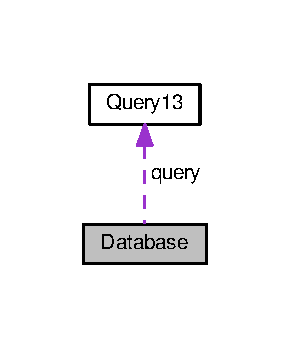
\includegraphics[width=139pt]{classDatabase__coll__graph}
\end{center}
\end{figure}
\subsection*{Public Member Functions}
\begin{DoxyCompactItemize}
\item 
\hyperlink{classDatabase_a5383fafec5ba098dc8c0415fab61ad84}{Database} (String filename, \hyperlink{interfaceQuery13}{Query13} \+\_\+query)
\item 
void \hyperlink{classDatabase_a3e1bf8d878423f430f63263f22e30013}{check} (\hyperlink{classDataRecords}{Data\+Records} d)
\end{DoxyCompactItemize}
\subsection*{Private Attributes}
\begin{DoxyCompactItemize}
\item 
S\+A\+X\+Parser \hyperlink{classDatabase_a484efd6d296ceb5ae434253519632980}{parser}
\item 
\hyperlink{interfaceQuery13}{Query13} \hyperlink{classDatabase_ae6f7784250367e1154d766eb3192e38f}{query}
\end{DoxyCompactItemize}


\subsection{Detailed Description}
This Class helps extracting relevant data 

\subsection{Constructor \& Destructor Documentation}
\index{Database@{Database}!Database@{Database}}
\index{Database@{Database}!Database@{Database}}
\subsubsection[{\texorpdfstring{Database(\+String filename, Query13 \+\_\+query)}{Database(String filename, Query13 _query)}}]{\setlength{\rightskip}{0pt plus 5cm}Database.\+Database (
\begin{DoxyParamCaption}
\item[{String}]{filename, }
\item[{{\bf Query13}}]{\+\_\+query}
\end{DoxyParamCaption}
)\hspace{0.3cm}{\ttfamily [inline]}}\hypertarget{classDatabase_a5383fafec5ba098dc8c0415fab61ad84}{}\label{classDatabase_a5383fafec5ba098dc8c0415fab61ad84}

\begin{DoxyCode}
16                                                     \{
17         \textcolor{keywordflow}{try}\{
18             \hyperlink{classDatabase_ae6f7784250367e1154d766eb3192e38f}{query} = \_query;
19             SAXParserFactory factory = SAXParserFactory.newInstance();
20             \hyperlink{classDatabase_a484efd6d296ceb5ae434253519632980}{parser} = factory.newSAXParser();
21             Handler handle = \textcolor{keyword}{new} Handler(\textcolor{keyword}{this});
22             \hyperlink{classDatabase_a484efd6d296ceb5ae434253519632980}{parser}.parse(filename, handle);
23         \}
24         \textcolor{keywordflow}{catch}(Exception e)\{
25             e.printStackTrace();
26         \}
27     \}
\end{DoxyCode}


\subsection{Member Function Documentation}
\index{Database@{Database}!check@{check}}
\index{check@{check}!Database@{Database}}
\subsubsection[{\texorpdfstring{check(\+Data\+Records d)}{check(DataRecords d)}}]{\setlength{\rightskip}{0pt plus 5cm}void Database.\+check (
\begin{DoxyParamCaption}
\item[{{\bf Data\+Records}}]{d}
\end{DoxyParamCaption}
)\hspace{0.3cm}{\ttfamily [inline]}}\hypertarget{classDatabase_a3e1bf8d878423f430f63263f22e30013}{}\label{classDatabase_a3e1bf8d878423f430f63263f22e30013}

\begin{DoxyCode}
28                                     \{
29         \hyperlink{classDatabase_ae6f7784250367e1154d766eb3192e38f}{query}.\hyperlink{interfaceQuery13_aa8625da54bbd25beb6968df65fe05e57}{check}(d);
30     \}
\end{DoxyCode}


\subsection{Member Data Documentation}
\index{Database@{Database}!parser@{parser}}
\index{parser@{parser}!Database@{Database}}
\subsubsection[{\texorpdfstring{parser}{parser}}]{\setlength{\rightskip}{0pt plus 5cm}S\+A\+X\+Parser Database.\+parser\hspace{0.3cm}{\ttfamily [private]}}\hypertarget{classDatabase_a484efd6d296ceb5ae434253519632980}{}\label{classDatabase_a484efd6d296ceb5ae434253519632980}
\index{Database@{Database}!query@{query}}
\index{query@{query}!Database@{Database}}
\subsubsection[{\texorpdfstring{query}{query}}]{\setlength{\rightskip}{0pt plus 5cm}{\bf Query13} Database.\+query\hspace{0.3cm}{\ttfamily [private]}}\hypertarget{classDatabase_ae6f7784250367e1154d766eb3192e38f}{}\label{classDatabase_ae6f7784250367e1154d766eb3192e38f}


The documentation for this class was generated from the following file\+:\begin{DoxyCompactItemize}
\item 
\hyperlink{Database_8java}{Database.\+java}\end{DoxyCompactItemize}

\hypertarget{classDataRecords}{}\section{Data\+Records Class Reference}
\label{classDataRecords}\index{Data\+Records@{Data\+Records}}


Inheritance diagram for Data\+Records\+:\nopagebreak
\begin{figure}[H]
\begin{center}
\leavevmode
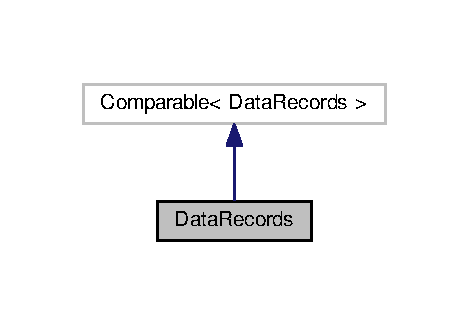
\includegraphics[width=225pt]{classDataRecords__inherit__graph}
\end{center}
\end{figure}


Collaboration diagram for Data\+Records\+:\nopagebreak
\begin{figure}[H]
\begin{center}
\leavevmode
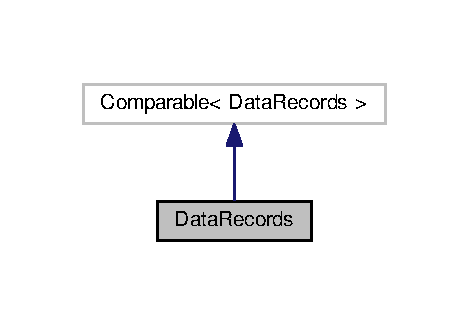
\includegraphics[width=225pt]{classDataRecords__coll__graph}
\end{center}
\end{figure}
\subsection*{Public Member Functions}
\begin{DoxyCompactItemize}
\item 
\hyperlink{classDataRecords_a793695c48b7a584d447facf8a0f36bbb}{Data\+Records} (String \+\_\+author, String \+\_\+title, String \+\_\+pages, String \+\_\+volume, String \+\_\+year, String \+\_\+journal, String \+\_\+booktitle, String \+\_\+url)
\item 
int \hyperlink{classDataRecords_a94e4170d60a20f3ccbe9ca53b69decef}{compare\+To} (\hyperlink{classDataRecords}{Data\+Records} d2)
\item 
boolean \hyperlink{classDataRecords_ad01e27f88e67399ad7a861616b65c523}{equals} (\hyperlink{classDataRecords}{Data\+Records} d2)
\item 
String \hyperlink{classDataRecords_a9b0dba84ec8d539395853caff7d4080f}{get\+Author} ()
\item 
String \hyperlink{classDataRecords_a2b6d27b078eb3a16734562f9ded6e1c6}{get\+Title} ()
\item 
String \hyperlink{classDataRecords_a484260b5897ee754d22bdb1e0b1a4d69}{get\+Pages} ()
\item 
String \hyperlink{classDataRecords_a6dfac293f0bd901eebf3a6ae17dc2513}{get\+Volume} ()
\item 
int \hyperlink{classDataRecords_a9918de1a257be6b753ef46d66c43989c}{get\+Year} ()
\item 
String \hyperlink{classDataRecords_aab28a326b036a7f0a8c041419c1c2382}{get\+Journal} ()
\item 
String \hyperlink{classDataRecords_a4c25863961be4da93a129474387c4f41}{get\+Book\+Title} ()
\item 
String \hyperlink{classDataRecords_add5c32b5a1511c42f70846fe08a4cfd7}{get\+Journal\+Title} ()
\item 
String \hyperlink{classDataRecords_a40351f370945cfa624e1e3e1d6addc3e}{get\+U\+RL} ()
\item 
int \hyperlink{classDataRecords_a7487a30fa32c0f7e8a05f26b6f23f25a}{get\+String\+Match} ()
\item 
void \hyperlink{classDataRecords_a1e41c4c115595d47b7bbf4016919ff8c}{set\+String\+Match} (int m)
\end{DoxyCompactItemize}
\subsection*{Private Attributes}
\begin{DoxyCompactItemize}
\item 
String \hyperlink{classDataRecords_a16230e6e4a7ff8947225b5336f34b727}{author}
\item 
String \hyperlink{classDataRecords_a0d2a944285b7168f1cc61f2173a3892b}{title}
\item 
String \hyperlink{classDataRecords_ad4ecb52d88a34679b11d9473acfca9f7}{pages}
\item 
int \hyperlink{classDataRecords_ad7124e534dcce1adc70799071c64e431}{year}
\item 
String \hyperlink{classDataRecords_a9def6bcb60fe42b44e052ebd5d499ac4}{volume}
\item 
String \hyperlink{classDataRecords_a89f32013b5ffe93fe421f7ad37534086}{journal}
\item 
String \hyperlink{classDataRecords_ad43b933314b398e13701deb18add0d49}{booktitle}
\item 
String \hyperlink{classDataRecords_a220ad19762fcd3d7eb0c7da32a75ab39}{url}
\item 
int \hyperlink{classDataRecords_a45d9849a7089e7461c8e5568ee0cac20}{string\+Match}
\end{DoxyCompactItemize}


\subsection{Detailed Description}
\hyperlink{classDataRecords}{Data\+Records} store all info related to a Publication 

\subsection{Constructor \& Destructor Documentation}
\index{Data\+Records@{Data\+Records}!Data\+Records@{Data\+Records}}
\index{Data\+Records@{Data\+Records}!Data\+Records@{Data\+Records}}
\subsubsection[{\texorpdfstring{Data\+Records(\+String \+\_\+author, String \+\_\+title, String \+\_\+pages, String \+\_\+volume, String \+\_\+year, String \+\_\+journal, String \+\_\+booktitle, String \+\_\+url)}{DataRecords(String _author, String _title, String _pages, String _volume, String _year, String _journal, String _booktitle, String _url)}}]{\setlength{\rightskip}{0pt plus 5cm}Data\+Records.\+Data\+Records (
\begin{DoxyParamCaption}
\item[{String}]{\+\_\+author, }
\item[{String}]{\+\_\+title, }
\item[{String}]{\+\_\+pages, }
\item[{String}]{\+\_\+volume, }
\item[{String}]{\+\_\+year, }
\item[{String}]{\+\_\+journal, }
\item[{String}]{\+\_\+booktitle, }
\item[{String}]{\+\_\+url}
\end{DoxyParamCaption}
)\hspace{0.3cm}{\ttfamily [inline]}}\hypertarget{classDataRecords_a793695c48b7a584d447facf8a0f36bbb}{}\label{classDataRecords_a793695c48b7a584d447facf8a0f36bbb}

\begin{DoxyCode}
20                                                                                                            
                                              \{
21         \hyperlink{classDataRecords_a16230e6e4a7ff8947225b5336f34b727}{author} = \_author;
22         \hyperlink{classDataRecords_a0d2a944285b7168f1cc61f2173a3892b}{title} = \_title;
23         \hyperlink{classDataRecords_ad4ecb52d88a34679b11d9473acfca9f7}{pages} = \_pages;
24         \hyperlink{classDataRecords_a9def6bcb60fe42b44e052ebd5d499ac4}{volume} = \_volume;
25         \textcolor{keywordflow}{try}\{    
26             \hyperlink{classDataRecords_ad7124e534dcce1adc70799071c64e431}{year} = Integer.parseInt(\_year);
27         \}
28         \textcolor{keywordflow}{catch} (Exception e)\{
29             \hyperlink{classDataRecords_ad7124e534dcce1adc70799071c64e431}{year} = 0;
30         \}
31         \hyperlink{classDataRecords_a89f32013b5ffe93fe421f7ad37534086}{journal} = \_journal;
32         \hyperlink{classDataRecords_ad43b933314b398e13701deb18add0d49}{booktitle} = \_booktitle;
33         \hyperlink{classDataRecords_a220ad19762fcd3d7eb0c7da32a75ab39}{url} = \_url;
34         \hyperlink{classDataRecords_a45d9849a7089e7461c8e5568ee0cac20}{stringMatch}=0;
35     \}
\end{DoxyCode}


\subsection{Member Function Documentation}
\index{Data\+Records@{Data\+Records}!compare\+To@{compare\+To}}
\index{compare\+To@{compare\+To}!Data\+Records@{Data\+Records}}
\subsubsection[{\texorpdfstring{compare\+To(\+Data\+Records d2)}{compareTo(DataRecords d2)}}]{\setlength{\rightskip}{0pt plus 5cm}int Data\+Records.\+compare\+To (
\begin{DoxyParamCaption}
\item[{{\bf Data\+Records}}]{d2}
\end{DoxyParamCaption}
)\hspace{0.3cm}{\ttfamily [inline]}}\hypertarget{classDataRecords_a94e4170d60a20f3ccbe9ca53b69decef}{}\label{classDataRecords_a94e4170d60a20f3ccbe9ca53b69decef}

\begin{DoxyCode}
36                                         \{
37         \textcolor{keywordflow}{if} (d2.\hyperlink{classDataRecords_a9918de1a257be6b753ef46d66c43989c}{getYear}() > \hyperlink{classDataRecords_ad7124e534dcce1adc70799071c64e431}{year})\{
38             \textcolor{keywordflow}{return} 1;
39         \}
40         \textcolor{keywordflow}{else} \textcolor{keywordflow}{if} (d2.\hyperlink{classDataRecords_a9918de1a257be6b753ef46d66c43989c}{getYear}() == \hyperlink{classDataRecords_ad7124e534dcce1adc70799071c64e431}{year})\{
41             \textcolor{keywordflow}{return} 0;
42         \}
43         \textcolor{keywordflow}{return} -1;
44     \}
\end{DoxyCode}
\index{Data\+Records@{Data\+Records}!equals@{equals}}
\index{equals@{equals}!Data\+Records@{Data\+Records}}
\subsubsection[{\texorpdfstring{equals(\+Data\+Records d2)}{equals(DataRecords d2)}}]{\setlength{\rightskip}{0pt plus 5cm}boolean Data\+Records.\+equals (
\begin{DoxyParamCaption}
\item[{{\bf Data\+Records}}]{d2}
\end{DoxyParamCaption}
)\hspace{0.3cm}{\ttfamily [inline]}}\hypertarget{classDataRecords_ad01e27f88e67399ad7a861616b65c523}{}\label{classDataRecords_ad01e27f88e67399ad7a861616b65c523}

\begin{DoxyCode}
45                                          \{
46         \textcolor{keywordflow}{return} d2.\hyperlink{classDataRecords_a9918de1a257be6b753ef46d66c43989c}{getYear}() == \hyperlink{classDataRecords_ad7124e534dcce1adc70799071c64e431}{year};
47     \}
\end{DoxyCode}
\index{Data\+Records@{Data\+Records}!get\+Author@{get\+Author}}
\index{get\+Author@{get\+Author}!Data\+Records@{Data\+Records}}
\subsubsection[{\texorpdfstring{get\+Author()}{getAuthor()}}]{\setlength{\rightskip}{0pt plus 5cm}String Data\+Records.\+get\+Author (
\begin{DoxyParamCaption}
{}
\end{DoxyParamCaption}
)\hspace{0.3cm}{\ttfamily [inline]}}\hypertarget{classDataRecords_a9b0dba84ec8d539395853caff7d4080f}{}\label{classDataRecords_a9b0dba84ec8d539395853caff7d4080f}

\begin{DoxyCode}
48                              \{
49         \textcolor{keywordflow}{return} \hyperlink{classDataRecords_a16230e6e4a7ff8947225b5336f34b727}{author};
50     \}
\end{DoxyCode}
\index{Data\+Records@{Data\+Records}!get\+Book\+Title@{get\+Book\+Title}}
\index{get\+Book\+Title@{get\+Book\+Title}!Data\+Records@{Data\+Records}}
\subsubsection[{\texorpdfstring{get\+Book\+Title()}{getBookTitle()}}]{\setlength{\rightskip}{0pt plus 5cm}String Data\+Records.\+get\+Book\+Title (
\begin{DoxyParamCaption}
{}
\end{DoxyParamCaption}
)\hspace{0.3cm}{\ttfamily [inline]}}\hypertarget{classDataRecords_a4c25863961be4da93a129474387c4f41}{}\label{classDataRecords_a4c25863961be4da93a129474387c4f41}

\begin{DoxyCode}
66                                 \{
67         \textcolor{keywordflow}{return} \hyperlink{classDataRecords_ad43b933314b398e13701deb18add0d49}{booktitle};
68     \}
\end{DoxyCode}
\index{Data\+Records@{Data\+Records}!get\+Journal@{get\+Journal}}
\index{get\+Journal@{get\+Journal}!Data\+Records@{Data\+Records}}
\subsubsection[{\texorpdfstring{get\+Journal()}{getJournal()}}]{\setlength{\rightskip}{0pt plus 5cm}String Data\+Records.\+get\+Journal (
\begin{DoxyParamCaption}
{}
\end{DoxyParamCaption}
)\hspace{0.3cm}{\ttfamily [inline]}}\hypertarget{classDataRecords_aab28a326b036a7f0a8c041419c1c2382}{}\label{classDataRecords_aab28a326b036a7f0a8c041419c1c2382}

\begin{DoxyCode}
63                               \{
64         \textcolor{keywordflow}{return} \hyperlink{classDataRecords_a89f32013b5ffe93fe421f7ad37534086}{journal};
65     \}
\end{DoxyCode}
\index{Data\+Records@{Data\+Records}!get\+Journal\+Title@{get\+Journal\+Title}}
\index{get\+Journal\+Title@{get\+Journal\+Title}!Data\+Records@{Data\+Records}}
\subsubsection[{\texorpdfstring{get\+Journal\+Title()}{getJournalTitle()}}]{\setlength{\rightskip}{0pt plus 5cm}String Data\+Records.\+get\+Journal\+Title (
\begin{DoxyParamCaption}
{}
\end{DoxyParamCaption}
)\hspace{0.3cm}{\ttfamily [inline]}}\hypertarget{classDataRecords_add5c32b5a1511c42f70846fe08a4cfd7}{}\label{classDataRecords_add5c32b5a1511c42f70846fe08a4cfd7}

\begin{DoxyCode}
69                                    \{
70         \textcolor{keywordflow}{if} (\hyperlink{classDataRecords_a89f32013b5ffe93fe421f7ad37534086}{journal} == null)\{
71             \textcolor{keywordflow}{return} \hyperlink{classDataRecords_ad43b933314b398e13701deb18add0d49}{booktitle};
72         \}
73         \textcolor{keywordflow}{return} \hyperlink{classDataRecords_a89f32013b5ffe93fe421f7ad37534086}{journal};
74     \}
\end{DoxyCode}
\index{Data\+Records@{Data\+Records}!get\+Pages@{get\+Pages}}
\index{get\+Pages@{get\+Pages}!Data\+Records@{Data\+Records}}
\subsubsection[{\texorpdfstring{get\+Pages()}{getPages()}}]{\setlength{\rightskip}{0pt plus 5cm}String Data\+Records.\+get\+Pages (
\begin{DoxyParamCaption}
{}
\end{DoxyParamCaption}
)\hspace{0.3cm}{\ttfamily [inline]}}\hypertarget{classDataRecords_a484260b5897ee754d22bdb1e0b1a4d69}{}\label{classDataRecords_a484260b5897ee754d22bdb1e0b1a4d69}

\begin{DoxyCode}
54                             \{
55         \textcolor{keywordflow}{return} \hyperlink{classDataRecords_ad4ecb52d88a34679b11d9473acfca9f7}{pages};
56     \}
\end{DoxyCode}
\index{Data\+Records@{Data\+Records}!get\+String\+Match@{get\+String\+Match}}
\index{get\+String\+Match@{get\+String\+Match}!Data\+Records@{Data\+Records}}
\subsubsection[{\texorpdfstring{get\+String\+Match()}{getStringMatch()}}]{\setlength{\rightskip}{0pt plus 5cm}int Data\+Records.\+get\+String\+Match (
\begin{DoxyParamCaption}
{}
\end{DoxyParamCaption}
)\hspace{0.3cm}{\ttfamily [inline]}}\hypertarget{classDataRecords_a7487a30fa32c0f7e8a05f26b6f23f25a}{}\label{classDataRecords_a7487a30fa32c0f7e8a05f26b6f23f25a}

\begin{DoxyCode}
79     \{
80         \textcolor{keywordflow}{return} \hyperlink{classDataRecords_a45d9849a7089e7461c8e5568ee0cac20}{stringMatch};
81     \}
\end{DoxyCode}
\index{Data\+Records@{Data\+Records}!get\+Title@{get\+Title}}
\index{get\+Title@{get\+Title}!Data\+Records@{Data\+Records}}
\subsubsection[{\texorpdfstring{get\+Title()}{getTitle()}}]{\setlength{\rightskip}{0pt plus 5cm}String Data\+Records.\+get\+Title (
\begin{DoxyParamCaption}
{}
\end{DoxyParamCaption}
)\hspace{0.3cm}{\ttfamily [inline]}}\hypertarget{classDataRecords_a2b6d27b078eb3a16734562f9ded6e1c6}{}\label{classDataRecords_a2b6d27b078eb3a16734562f9ded6e1c6}

\begin{DoxyCode}
51                             \{
52         \textcolor{keywordflow}{return} \hyperlink{classDataRecords_a0d2a944285b7168f1cc61f2173a3892b}{title};
53     \}
\end{DoxyCode}
\index{Data\+Records@{Data\+Records}!get\+U\+RL@{get\+U\+RL}}
\index{get\+U\+RL@{get\+U\+RL}!Data\+Records@{Data\+Records}}
\subsubsection[{\texorpdfstring{get\+U\+R\+L()}{getURL()}}]{\setlength{\rightskip}{0pt plus 5cm}String Data\+Records.\+get\+U\+RL (
\begin{DoxyParamCaption}
{}
\end{DoxyParamCaption}
)\hspace{0.3cm}{\ttfamily [inline]}}\hypertarget{classDataRecords_a40351f370945cfa624e1e3e1d6addc3e}{}\label{classDataRecords_a40351f370945cfa624e1e3e1d6addc3e}

\begin{DoxyCode}
75                           \{
76         \textcolor{keywordflow}{return} \hyperlink{classDataRecords_a220ad19762fcd3d7eb0c7da32a75ab39}{url};
77     \}
\end{DoxyCode}
\index{Data\+Records@{Data\+Records}!get\+Volume@{get\+Volume}}
\index{get\+Volume@{get\+Volume}!Data\+Records@{Data\+Records}}
\subsubsection[{\texorpdfstring{get\+Volume()}{getVolume()}}]{\setlength{\rightskip}{0pt plus 5cm}String Data\+Records.\+get\+Volume (
\begin{DoxyParamCaption}
{}
\end{DoxyParamCaption}
)\hspace{0.3cm}{\ttfamily [inline]}}\hypertarget{classDataRecords_a6dfac293f0bd901eebf3a6ae17dc2513}{}\label{classDataRecords_a6dfac293f0bd901eebf3a6ae17dc2513}

\begin{DoxyCode}
57                              \{
58         \textcolor{keywordflow}{return} \hyperlink{classDataRecords_a9def6bcb60fe42b44e052ebd5d499ac4}{volume};
59     \}
\end{DoxyCode}
\index{Data\+Records@{Data\+Records}!get\+Year@{get\+Year}}
\index{get\+Year@{get\+Year}!Data\+Records@{Data\+Records}}
\subsubsection[{\texorpdfstring{get\+Year()}{getYear()}}]{\setlength{\rightskip}{0pt plus 5cm}int Data\+Records.\+get\+Year (
\begin{DoxyParamCaption}
{}
\end{DoxyParamCaption}
)\hspace{0.3cm}{\ttfamily [inline]}}\hypertarget{classDataRecords_a9918de1a257be6b753ef46d66c43989c}{}\label{classDataRecords_a9918de1a257be6b753ef46d66c43989c}

\begin{DoxyCode}
60                         \{
61         \textcolor{keywordflow}{return} \hyperlink{classDataRecords_ad7124e534dcce1adc70799071c64e431}{year};
62     \}
\end{DoxyCode}
\index{Data\+Records@{Data\+Records}!set\+String\+Match@{set\+String\+Match}}
\index{set\+String\+Match@{set\+String\+Match}!Data\+Records@{Data\+Records}}
\subsubsection[{\texorpdfstring{set\+String\+Match(int m)}{setStringMatch(int m)}}]{\setlength{\rightskip}{0pt plus 5cm}void Data\+Records.\+set\+String\+Match (
\begin{DoxyParamCaption}
\item[{int}]{m}
\end{DoxyParamCaption}
)\hspace{0.3cm}{\ttfamily [inline]}}\hypertarget{classDataRecords_a1e41c4c115595d47b7bbf4016919ff8c}{}\label{classDataRecords_a1e41c4c115595d47b7bbf4016919ff8c}

\begin{DoxyCode}
83     \{
84         \hyperlink{classDataRecords_a45d9849a7089e7461c8e5568ee0cac20}{stringMatch}=m;
85     \}
\end{DoxyCode}


\subsection{Member Data Documentation}
\index{Data\+Records@{Data\+Records}!author@{author}}
\index{author@{author}!Data\+Records@{Data\+Records}}
\subsubsection[{\texorpdfstring{author}{author}}]{\setlength{\rightskip}{0pt plus 5cm}String Data\+Records.\+author\hspace{0.3cm}{\ttfamily [private]}}\hypertarget{classDataRecords_a16230e6e4a7ff8947225b5336f34b727}{}\label{classDataRecords_a16230e6e4a7ff8947225b5336f34b727}
\index{Data\+Records@{Data\+Records}!booktitle@{booktitle}}
\index{booktitle@{booktitle}!Data\+Records@{Data\+Records}}
\subsubsection[{\texorpdfstring{booktitle}{booktitle}}]{\setlength{\rightskip}{0pt plus 5cm}String Data\+Records.\+booktitle\hspace{0.3cm}{\ttfamily [private]}}\hypertarget{classDataRecords_ad43b933314b398e13701deb18add0d49}{}\label{classDataRecords_ad43b933314b398e13701deb18add0d49}
\index{Data\+Records@{Data\+Records}!journal@{journal}}
\index{journal@{journal}!Data\+Records@{Data\+Records}}
\subsubsection[{\texorpdfstring{journal}{journal}}]{\setlength{\rightskip}{0pt plus 5cm}String Data\+Records.\+journal\hspace{0.3cm}{\ttfamily [private]}}\hypertarget{classDataRecords_a89f32013b5ffe93fe421f7ad37534086}{}\label{classDataRecords_a89f32013b5ffe93fe421f7ad37534086}
\index{Data\+Records@{Data\+Records}!pages@{pages}}
\index{pages@{pages}!Data\+Records@{Data\+Records}}
\subsubsection[{\texorpdfstring{pages}{pages}}]{\setlength{\rightskip}{0pt plus 5cm}String Data\+Records.\+pages\hspace{0.3cm}{\ttfamily [private]}}\hypertarget{classDataRecords_ad4ecb52d88a34679b11d9473acfca9f7}{}\label{classDataRecords_ad4ecb52d88a34679b11d9473acfca9f7}
\index{Data\+Records@{Data\+Records}!string\+Match@{string\+Match}}
\index{string\+Match@{string\+Match}!Data\+Records@{Data\+Records}}
\subsubsection[{\texorpdfstring{string\+Match}{stringMatch}}]{\setlength{\rightskip}{0pt plus 5cm}int Data\+Records.\+string\+Match\hspace{0.3cm}{\ttfamily [private]}}\hypertarget{classDataRecords_a45d9849a7089e7461c8e5568ee0cac20}{}\label{classDataRecords_a45d9849a7089e7461c8e5568ee0cac20}
\index{Data\+Records@{Data\+Records}!title@{title}}
\index{title@{title}!Data\+Records@{Data\+Records}}
\subsubsection[{\texorpdfstring{title}{title}}]{\setlength{\rightskip}{0pt plus 5cm}String Data\+Records.\+title\hspace{0.3cm}{\ttfamily [private]}}\hypertarget{classDataRecords_a0d2a944285b7168f1cc61f2173a3892b}{}\label{classDataRecords_a0d2a944285b7168f1cc61f2173a3892b}
\index{Data\+Records@{Data\+Records}!url@{url}}
\index{url@{url}!Data\+Records@{Data\+Records}}
\subsubsection[{\texorpdfstring{url}{url}}]{\setlength{\rightskip}{0pt plus 5cm}String Data\+Records.\+url\hspace{0.3cm}{\ttfamily [private]}}\hypertarget{classDataRecords_a220ad19762fcd3d7eb0c7da32a75ab39}{}\label{classDataRecords_a220ad19762fcd3d7eb0c7da32a75ab39}
\index{Data\+Records@{Data\+Records}!volume@{volume}}
\index{volume@{volume}!Data\+Records@{Data\+Records}}
\subsubsection[{\texorpdfstring{volume}{volume}}]{\setlength{\rightskip}{0pt plus 5cm}String Data\+Records.\+volume\hspace{0.3cm}{\ttfamily [private]}}\hypertarget{classDataRecords_a9def6bcb60fe42b44e052ebd5d499ac4}{}\label{classDataRecords_a9def6bcb60fe42b44e052ebd5d499ac4}
\index{Data\+Records@{Data\+Records}!year@{year}}
\index{year@{year}!Data\+Records@{Data\+Records}}
\subsubsection[{\texorpdfstring{year}{year}}]{\setlength{\rightskip}{0pt plus 5cm}int Data\+Records.\+year\hspace{0.3cm}{\ttfamily [private]}}\hypertarget{classDataRecords_ad7124e534dcce1adc70799071c64e431}{}\label{classDataRecords_ad7124e534dcce1adc70799071c64e431}


The documentation for this class was generated from the following file\+:\begin{DoxyCompactItemize}
\item 
\hyperlink{DataRecords_8java}{Data\+Records.\+java}\end{DoxyCompactItemize}

\hypertarget{classGUI}{}\section{G\+UI Class Reference}
\label{classGUI}\index{G\+UI@{G\+UI}}


Collaboration diagram for G\+UI\+:\nopagebreak
\begin{figure}[H]
\begin{center}
\leavevmode
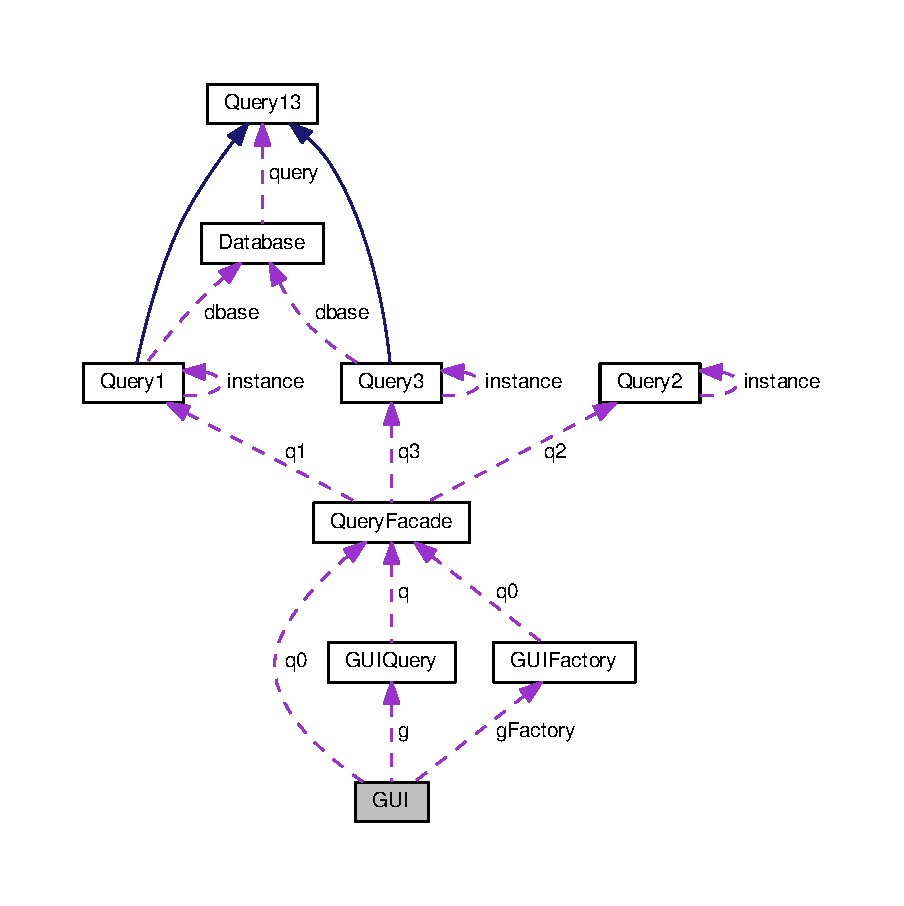
\includegraphics[width=350pt]{classGUI__coll__graph}
\end{center}
\end{figure}
\subsection*{Public Member Functions}
\begin{DoxyCompactItemize}
\item 
\hyperlink{classGUI_a35a15f9dcfca9111335e4401a46567ed}{G\+UI} ()
\item 
void \hyperlink{classGUI_a23acbb0a9e9350e946407b677e88b5b5}{run\+Frame} ()
\item 
void \hyperlink{classGUI_a110149939fa2b371bcc1f86b15aa2f63}{initframe} ()
\item 
void \hyperlink{classGUI_aff3d813da1e25b7926c7b340ed57009b}{change} (int i)
\item 
void \hyperlink{classGUI_a2ecefd4112807c7f4d96e49b1cf0a46c}{change\+Mode} (int i)
\end{DoxyCompactItemize}
\subsection*{Static Public Member Functions}
\begin{DoxyCompactItemize}
\item 
static void \hyperlink{classGUI_a8202c223d5b25c7dd94ce70bd6a267ac}{main} (String\mbox{[}$\,$\mbox{]} args)
\item 
static boolean \hyperlink{classGUI_a0ec9bf129676c56850ebc391c4c4b54e}{is\+Integer} (String s)
\end{DoxyCompactItemize}
\subsection*{Private Attributes}
\begin{DoxyCompactItemize}
\item 
J\+Frame \hyperlink{classGUI_ad0edd6841874d6f0d4d92b38fe4c58fa}{main\+Frame}
\item 
J\+Panel \hyperlink{classGUI_a5ae695a244b7bf0e35c5387063d0a6ae}{upper\+Panel}
\item 
J\+Panel \hyperlink{classGUI_a6930a3cfc244b0ce0d03e3fab60d33c7}{side\+Panel}
\item 
J\+Panel \hyperlink{classGUI_aa88e747a84e0e3b6ba35371f007c8151}{display\+Panel}
\item 
J\+Combo\+Box$<$ String $>$ \hyperlink{classGUI_ac15dd4c4cf3422b2e3ad7209b70b2df2}{queries}
\item 
J\+Button \hyperlink{classGUI_a4a469da0727abf52b86e23b12ca91fc6}{submit}
\item 
\hyperlink{classGUIQuery}{G\+U\+I\+Query} \hyperlink{classGUI_a267a714cad7b99c5f450e33e2bd91d0d}{g}
\item 
\hyperlink{classGUIFactory}{G\+U\+I\+Factory} \hyperlink{classGUI_ac95015c84714d8ba5c83e4a875466785}{g\+Factory}
\item 
\hyperlink{classQueryFacade}{Query\+Facade} \hyperlink{classGUI_a55cc973319a37d99e306b0c8cc665269}{q0} = new \hyperlink{classQueryFacade}{Query\+Facade}()
\item 
int \hyperlink{classGUI_a268ed195698683851c5ae951338182d1}{flag} =0
\end{DoxyCompactItemize}


\subsection{Detailed Description}
Contains the base \hyperlink{classGUI}{G\+UI} class that loads the frame, also contains the projects main 

\subsection{Constructor \& Destructor Documentation}
\index{G\+UI@{G\+UI}!G\+UI@{G\+UI}}
\index{G\+UI@{G\+UI}!G\+UI@{G\+UI}}
\subsubsection[{\texorpdfstring{G\+U\+I()}{GUI()}}]{\setlength{\rightskip}{0pt plus 5cm}G\+U\+I.\+G\+UI (
\begin{DoxyParamCaption}
{}
\end{DoxyParamCaption}
)\hspace{0.3cm}{\ttfamily [inline]}}\hypertarget{classGUI_a35a15f9dcfca9111335e4401a46567ed}{}\label{classGUI_a35a15f9dcfca9111335e4401a46567ed}

\begin{DoxyCode}
32     \{
33         \hyperlink{classGUI_a23acbb0a9e9350e946407b677e88b5b5}{runFrame}();
34         \hyperlink{classGUI_a110149939fa2b371bcc1f86b15aa2f63}{initframe}();
35     \}
\end{DoxyCode}


\subsection{Member Function Documentation}
\index{G\+UI@{G\+UI}!change@{change}}
\index{change@{change}!G\+UI@{G\+UI}}
\subsubsection[{\texorpdfstring{change(int i)}{change(int i)}}]{\setlength{\rightskip}{0pt plus 5cm}void G\+U\+I.\+change (
\begin{DoxyParamCaption}
\item[{int}]{i}
\end{DoxyParamCaption}
)\hspace{0.3cm}{\ttfamily [inline]}}\hypertarget{classGUI_aff3d813da1e25b7926c7b340ed57009b}{}\label{classGUI_aff3d813da1e25b7926c7b340ed57009b}

\begin{DoxyCode}
135     \{
136         \hyperlink{classGUI_a268ed195698683851c5ae951338182d1}{flag}=i;
137     \}
\end{DoxyCode}
\index{G\+UI@{G\+UI}!change\+Mode@{change\+Mode}}
\index{change\+Mode@{change\+Mode}!G\+UI@{G\+UI}}
\subsubsection[{\texorpdfstring{change\+Mode(int i)}{changeMode(int i)}}]{\setlength{\rightskip}{0pt plus 5cm}void G\+U\+I.\+change\+Mode (
\begin{DoxyParamCaption}
\item[{int}]{i}
\end{DoxyParamCaption}
)\hspace{0.3cm}{\ttfamily [inline]}}\hypertarget{classGUI_a2ecefd4112807c7f4d96e49b1cf0a46c}{}\label{classGUI_a2ecefd4112807c7f4d96e49b1cf0a46c}

\begin{DoxyCode}
139     \{
140         flag2=i;
141     \}
\end{DoxyCode}
\index{G\+UI@{G\+UI}!initframe@{initframe}}
\index{initframe@{initframe}!G\+UI@{G\+UI}}
\subsubsection[{\texorpdfstring{initframe()}{initframe()}}]{\setlength{\rightskip}{0pt plus 5cm}void G\+U\+I.\+initframe (
\begin{DoxyParamCaption}
{}
\end{DoxyParamCaption}
)\hspace{0.3cm}{\ttfamily [inline]}}\hypertarget{classGUI_a110149939fa2b371bcc1f86b15aa2f63}{}\label{classGUI_a110149939fa2b371bcc1f86b15aa2f63}

\begin{DoxyCode}
79     \{
80         \hyperlink{classGUI_a6930a3cfc244b0ce0d03e3fab60d33c7}{sidePanel}.add(\hyperlink{classGUI_ac15dd4c4cf3422b2e3ad7209b70b2df2}{queries});
81         \hyperlink{classGUI_ac15dd4c4cf3422b2e3ad7209b70b2df2}{queries}.setBounds(50,100,100,20);
82         \hyperlink{classGUI_ac15dd4c4cf3422b2e3ad7209b70b2df2}{queries}.setAlignmentX(Component.CENTER\_ALIGNMENT);
83         JLabel random = \textcolor{keyword}{new} JLabel(\textcolor{stringliteral}{"Results Here"});
84         random.setBounds(150,100,150,40);
85         \hyperlink{classGUI_aa88e747a84e0e3b6ba35371f007c8151}{displayPanel}.add(random);
86         JLabel header=\textcolor{keyword}{new} JLabel(\textcolor{stringliteral}{"<html><b>DBLP Query Engine</b></html>"},JLabel.CENTER);
87         header.setFont(\textcolor{keyword}{new} Font(\textcolor{stringliteral}{"Calibri"}, Font.PLAIN, 45));
88         header.setBounds(200,10,500,60);
89         header.setAlignmentX(Component.CENTER\_ALIGNMENT);
90         \hyperlink{classGUI_a5ae695a244b7bf0e35c5387063d0a6ae}{upperPanel}.add(header);
91         \hyperlink{classGUI_a5ae695a244b7bf0e35c5387063d0a6ae}{upperPanel}.setBorder(BorderFactory.createLineBorder(Color.black,2));
92         \hyperlink{classGUI_a5ae695a244b7bf0e35c5387063d0a6ae}{upperPanel}.setBackground(Color.WHITE);
93         \hyperlink{classGUI_a6930a3cfc244b0ce0d03e3fab60d33c7}{sidePanel}.setVisible(\textcolor{keyword}{true});
94         \hyperlink{classGUI_a5ae695a244b7bf0e35c5387063d0a6ae}{upperPanel}.setVisible(\textcolor{keyword}{true});
95         \hyperlink{classGUI_aa88e747a84e0e3b6ba35371f007c8151}{displayPanel}.setVisible(\textcolor{keyword}{true});
96         \hyperlink{classGUI_a6930a3cfc244b0ce0d03e3fab60d33c7}{sidePanel}.setBounds(0,80,250,440);
97         \hyperlink{classGUI_a5ae695a244b7bf0e35c5387063d0a6ae}{upperPanel}.setBounds(0,0,1200,80);
98         \hyperlink{classGUI_aa88e747a84e0e3b6ba35371f007c8151}{displayPanel}.setBounds(250,80,950,440);
99         \hyperlink{classGUI_ad0edd6841874d6f0d4d92b38fe4c58fa}{mainFrame}.add(\hyperlink{classGUI_a6930a3cfc244b0ce0d03e3fab60d33c7}{sidePanel});
100         \hyperlink{classGUI_ad0edd6841874d6f0d4d92b38fe4c58fa}{mainFrame}.add(\hyperlink{classGUI_a5ae695a244b7bf0e35c5387063d0a6ae}{upperPanel});
101         \hyperlink{classGUI_ad0edd6841874d6f0d4d92b38fe4c58fa}{mainFrame}.add(\hyperlink{classGUI_aa88e747a84e0e3b6ba35371f007c8151}{displayPanel});
102         \hyperlink{classGUI_ad0edd6841874d6f0d4d92b38fe4c58fa}{mainFrame}.setVisible(\textcolor{keyword}{true}); 
103         \hyperlink{classGUI_ac95015c84714d8ba5c83e4a875466785}{gFactory} = \textcolor{keyword}{new} \hyperlink{classGUIFactory}{GUIFactory}(\hyperlink{classGUI_ad0edd6841874d6f0d4d92b38fe4c58fa}{mainFrame},\hyperlink{classGUI_ac15dd4c4cf3422b2e3ad7209b70b2df2}{queries},
      \hyperlink{classGUI_a6930a3cfc244b0ce0d03e3fab60d33c7}{sidePanel},\hyperlink{classGUI_aa88e747a84e0e3b6ba35371f007c8151}{displayPanel},\hyperlink{classGUI_a55cc973319a37d99e306b0c8cc665269}{q0});
104         \hyperlink{classGUI_ac15dd4c4cf3422b2e3ad7209b70b2df2}{queries}.addActionListener(\textcolor{keyword}{new} ActionListener() \{
105             @Override
106             \textcolor{keyword}{public} \textcolor{keywordtype}{void} actionPerformed(ActionEvent event) \{
107                     JComboBox<? extends Object> q = (JComboBox<? extends Object>) event.getSource();
108                 String selectedQuery = (String) q.getSelectedItem();
109                 \textcolor{keywordflow}{if} (selectedQuery.equals(\textcolor{stringliteral}{"Query 1"})) \{
110                    \hyperlink{classGUI_a267a714cad7b99c5f450e33e2bd91d0d}{g}=\hyperlink{classGUI_ac95015c84714d8ba5c83e4a875466785}{gFactory}.\hyperlink{classGUIFactory_a2b891d0369711430ae1d172f15b78317}{getQuery}(\textcolor{stringliteral}{"Query1"});
111                    \hyperlink{classGUI_a267a714cad7b99c5f450e33e2bd91d0d}{g}.\hyperlink{classGUIQuery_acc9553514ecac053151c7580b83dec21}{start}();
112                 \}     \textcolor{keywordflow}{else} \textcolor{keywordflow}{if} (selectedQuery.equals(\textcolor{stringliteral}{"Query 2"})) \{
113                     \hyperlink{classGUI_a267a714cad7b99c5f450e33e2bd91d0d}{g}=\hyperlink{classGUI_ac95015c84714d8ba5c83e4a875466785}{gFactory}.\hyperlink{classGUIFactory_a2b891d0369711430ae1d172f15b78317}{getQuery}(\textcolor{stringliteral}{"Query2"});
114                     \hyperlink{classGUI_a267a714cad7b99c5f450e33e2bd91d0d}{g}.\hyperlink{classGUIQuery_acc9553514ecac053151c7580b83dec21}{start}();
115                 \} \textcolor{keywordflow}{else} \textcolor{keywordflow}{if}(selectedQuery.equals(\textcolor{stringliteral}{"Query 3"})) \{
116                     \hyperlink{classGUI_a267a714cad7b99c5f450e33e2bd91d0d}{g}=\hyperlink{classGUI_ac95015c84714d8ba5c83e4a875466785}{gFactory}.\hyperlink{classGUIFactory_a2b891d0369711430ae1d172f15b78317}{getQuery}(\textcolor{stringliteral}{"Query3"});
117                     \hyperlink{classGUI_a267a714cad7b99c5f450e33e2bd91d0d}{g}.\hyperlink{classGUIQuery_acc9553514ecac053151c7580b83dec21}{start}();
118                 \}
119             \}
120         \});
121     \}
\end{DoxyCode}
\index{G\+UI@{G\+UI}!is\+Integer@{is\+Integer}}
\index{is\+Integer@{is\+Integer}!G\+UI@{G\+UI}}
\subsubsection[{\texorpdfstring{is\+Integer(\+String s)}{isInteger(String s)}}]{\setlength{\rightskip}{0pt plus 5cm}static boolean G\+U\+I.\+is\+Integer (
\begin{DoxyParamCaption}
\item[{String}]{s}
\end{DoxyParamCaption}
)\hspace{0.3cm}{\ttfamily [inline]}, {\ttfamily [static]}}\hypertarget{classGUI_a0ec9bf129676c56850ebc391c4c4b54e}{}\label{classGUI_a0ec9bf129676c56850ebc391c4c4b54e}

\begin{DoxyCode}
142                                               \{
143       \textcolor{keywordtype}{boolean} isValidInteger = \textcolor{keyword}{false};
144       \textcolor{keywordflow}{try}
145       \{
146          Integer.parseInt(s);
147          isValidInteger = \textcolor{keyword}{true};
148       \}
149       \textcolor{keywordflow}{catch} (NumberFormatException ex)
150       \{\}
151       \textcolor{keywordflow}{return} isValidInteger;
152    \}
\end{DoxyCode}
\index{G\+UI@{G\+UI}!main@{main}}
\index{main@{main}!G\+UI@{G\+UI}}
\subsubsection[{\texorpdfstring{main(\+String[] args)}{main(String[] args)}}]{\setlength{\rightskip}{0pt plus 5cm}static void G\+U\+I.\+main (
\begin{DoxyParamCaption}
\item[{String\mbox{[}$\,$\mbox{]}}]{args}
\end{DoxyParamCaption}
)\hspace{0.3cm}{\ttfamily [inline]}, {\ttfamily [static]}}\hypertarget{classGUI_a8202c223d5b25c7dd94ce70bd6a267ac}{}\label{classGUI_a8202c223d5b25c7dd94ce70bd6a267ac}

\begin{DoxyCode}
124     \{
125         System.setProperty(\textcolor{stringliteral}{"jdk.xml.entityExpansionLimit"}, \textcolor{stringliteral}{"0"});
126         \hyperlink{classAuthorManager}{AuthorManager}.\hyperlink{classAuthorManager_a2fd95ddd7a1565f7665a7d961b445788}{addFile}(\textcolor{stringliteral}{"dblp.xml"});
127         \hyperlink{classGuiLoading}{GuiLoading} gl = \textcolor{keyword}{new} \hyperlink{classGuiLoading}{GuiLoading}();
128         gl.\hyperlink{classGuiLoading_aa13c96669e7ef681bfeae1a5b2dfab85}{start}();
129         \hyperlink{classAuthorManager}{AuthorManager}.\hyperlink{classAuthorManager_ac6244bdca3be32f6037f5c045c69f6f5}{createMap}();
130         gl.\hyperlink{classGuiLoading_addd66da1f2d489192a2afdc66abef566}{stop}();
131         \hyperlink{classGUI}{GUI} a = \textcolor{keyword}{new} \hyperlink{classGUI_a35a15f9dcfca9111335e4401a46567ed}{GUI}();
132     \}
\end{DoxyCode}
\index{G\+UI@{G\+UI}!run\+Frame@{run\+Frame}}
\index{run\+Frame@{run\+Frame}!G\+UI@{G\+UI}}
\subsubsection[{\texorpdfstring{run\+Frame()}{runFrame()}}]{\setlength{\rightskip}{0pt plus 5cm}void G\+U\+I.\+run\+Frame (
\begin{DoxyParamCaption}
{}
\end{DoxyParamCaption}
)\hspace{0.3cm}{\ttfamily [inline]}}\hypertarget{classGUI_a23acbb0a9e9350e946407b677e88b5b5}{}\label{classGUI_a23acbb0a9e9350e946407b677e88b5b5}

\begin{DoxyCode}
38     \{
39         \hyperlink{classGUI_ad0edd6841874d6f0d4d92b38fe4c58fa}{mainFrame}=\textcolor{keyword}{new} JFrame(\textcolor{stringliteral}{"DBLP query engine"});
40         \hyperlink{classGUI_a4a469da0727abf52b86e23b12ca91fc6}{submit}=\textcolor{keyword}{new} JButton(\textcolor{stringliteral}{"Submit"});
41         reset=\textcolor{keyword}{new} JButton(\textcolor{stringliteral}{"Reset"});
42         \hyperlink{classGUI_a6930a3cfc244b0ce0d03e3fab60d33c7}{sidePanel}=\textcolor{keyword}{new} JPanel();
43         \hyperlink{classGUI_ac15dd4c4cf3422b2e3ad7209b70b2df2}{queries} = \textcolor{keyword}{new} JComboBox<String>();
44         \hyperlink{classGUI_aa88e747a84e0e3b6ba35371f007c8151}{displayPanel}=\textcolor{keyword}{new} JPanel();
45         \hyperlink{classGUI_ac15dd4c4cf3422b2e3ad7209b70b2df2}{queries}.addItem(\textcolor{stringliteral}{"Queries"});
46         \hyperlink{classGUI_ac15dd4c4cf3422b2e3ad7209b70b2df2}{queries}.addItem(\textcolor{stringliteral}{"Query 1"});
47         \hyperlink{classGUI_ac15dd4c4cf3422b2e3ad7209b70b2df2}{queries}.addItem(\textcolor{stringliteral}{"Query 2"});
48         \hyperlink{classGUI_ac15dd4c4cf3422b2e3ad7209b70b2df2}{queries}.addItem(\textcolor{stringliteral}{"Query 3"});
49         \hyperlink{classGUI_ad0edd6841874d6f0d4d92b38fe4c58fa}{mainFrame}.setSize(1200,520); 
50         \hyperlink{classGUI_ad0edd6841874d6f0d4d92b38fe4c58fa}{mainFrame}.setLocation(0,0);
51         \hyperlink{classGUI_ad0edd6841874d6f0d4d92b38fe4c58fa}{mainFrame}.setResizable(\textcolor{keyword}{false});
52         \hyperlink{classGUI_ad0edd6841874d6f0d4d92b38fe4c58fa}{mainFrame}.setLayout(null);
53         \hyperlink{classGUI_ad0edd6841874d6f0d4d92b38fe4c58fa}{mainFrame}.setDefaultCloseOperation(JFrame.EXIT\_ON\_CLOSE);
54         \hyperlink{classGUI_a4a469da0727abf52b86e23b12ca91fc6}{submit}.setBackground(Color.BLACK);
55         reset.setBackground(Color.RED);
56         \hyperlink{classGUI_a6930a3cfc244b0ce0d03e3fab60d33c7}{sidePanel}.setPreferredSize(\textcolor{keyword}{new} Dimension(250,440));
57         \hyperlink{classGUI_a6930a3cfc244b0ce0d03e3fab60d33c7}{sidePanel}.setMinimumSize(\textcolor{keyword}{new} Dimension(250,440));
58         \hyperlink{classGUI_a6930a3cfc244b0ce0d03e3fab60d33c7}{sidePanel}.setMaximumSize(\textcolor{keyword}{new} Dimension(250,440));
59         \hyperlink{classGUI_a6930a3cfc244b0ce0d03e3fab60d33c7}{sidePanel}.setLocation(0,80);
60         \hyperlink{classGUI_a6930a3cfc244b0ce0d03e3fab60d33c7}{sidePanel}.setLayout(null);
61         \hyperlink{classGUI_a6930a3cfc244b0ce0d03e3fab60d33c7}{sidePanel}.setBorder(BorderFactory.createLineBorder(Color.black,2));
62         \hyperlink{classGUI_a6930a3cfc244b0ce0d03e3fab60d33c7}{sidePanel}.setBackground(Color.WHITE);
63         displayPanel.setPreferredSize(\textcolor{keyword}{new} Dimension(950,440));
64         displayPanel.setMinimumSize(\textcolor{keyword}{new} Dimension(950,440));
65         displayPanel.setMaximumSize(\textcolor{keyword}{new} Dimension(950,440));
66         displayPanel.setLocation(250,80);
67         displayPanel.setLayout(null);
68         displayPanel.setBorder(BorderFactory.createLineBorder(Color.black,2));
69         displayPanel.setBackground(Color.WHITE);
70         \hyperlink{classGUI_a5ae695a244b7bf0e35c5387063d0a6ae}{upperPanel}=\textcolor{keyword}{new} JPanel();
71         \hyperlink{classGUI_a5ae695a244b7bf0e35c5387063d0a6ae}{upperPanel}.setSize(\textcolor{keyword}{new} Dimension(1200,80));
72         \hyperlink{classGUI_a5ae695a244b7bf0e35c5387063d0a6ae}{upperPanel}.setMinimumSize(\textcolor{keyword}{new} Dimension(1200,80));
73         \hyperlink{classGUI_a5ae695a244b7bf0e35c5387063d0a6ae}{upperPanel}.setMaximumSize(\textcolor{keyword}{new} Dimension(1200,80));
74         \hyperlink{classGUI_a5ae695a244b7bf0e35c5387063d0a6ae}{upperPanel}.setLocation(0,0);
75         \hyperlink{classGUI_a5ae695a244b7bf0e35c5387063d0a6ae}{upperPanel}.setLayout(null);
76     \}
\end{DoxyCode}


\subsection{Member Data Documentation}
\index{G\+UI@{G\+UI}!display\+Panel@{display\+Panel}}
\index{display\+Panel@{display\+Panel}!G\+UI@{G\+UI}}
\subsubsection[{\texorpdfstring{display\+Panel}{displayPanel}}]{\setlength{\rightskip}{0pt plus 5cm}J\+Panel G\+U\+I.\+display\+Panel\hspace{0.3cm}{\ttfamily [private]}}\hypertarget{classGUI_aa88e747a84e0e3b6ba35371f007c8151}{}\label{classGUI_aa88e747a84e0e3b6ba35371f007c8151}
\index{G\+UI@{G\+UI}!flag@{flag}}
\index{flag@{flag}!G\+UI@{G\+UI}}
\subsubsection[{\texorpdfstring{flag}{flag}}]{\setlength{\rightskip}{0pt plus 5cm}int G\+U\+I.\+flag =0\hspace{0.3cm}{\ttfamily [private]}}\hypertarget{classGUI_a268ed195698683851c5ae951338182d1}{}\label{classGUI_a268ed195698683851c5ae951338182d1}
\index{G\+UI@{G\+UI}!g@{g}}
\index{g@{g}!G\+UI@{G\+UI}}
\subsubsection[{\texorpdfstring{g}{g}}]{\setlength{\rightskip}{0pt plus 5cm}{\bf G\+U\+I\+Query} G\+U\+I.\+g\hspace{0.3cm}{\ttfamily [private]}}\hypertarget{classGUI_a267a714cad7b99c5f450e33e2bd91d0d}{}\label{classGUI_a267a714cad7b99c5f450e33e2bd91d0d}
\index{G\+UI@{G\+UI}!g\+Factory@{g\+Factory}}
\index{g\+Factory@{g\+Factory}!G\+UI@{G\+UI}}
\subsubsection[{\texorpdfstring{g\+Factory}{gFactory}}]{\setlength{\rightskip}{0pt plus 5cm}{\bf G\+U\+I\+Factory} G\+U\+I.\+g\+Factory\hspace{0.3cm}{\ttfamily [private]}}\hypertarget{classGUI_ac95015c84714d8ba5c83e4a875466785}{}\label{classGUI_ac95015c84714d8ba5c83e4a875466785}
\index{G\+UI@{G\+UI}!main\+Frame@{main\+Frame}}
\index{main\+Frame@{main\+Frame}!G\+UI@{G\+UI}}
\subsubsection[{\texorpdfstring{main\+Frame}{mainFrame}}]{\setlength{\rightskip}{0pt plus 5cm}J\+Frame G\+U\+I.\+main\+Frame\hspace{0.3cm}{\ttfamily [private]}}\hypertarget{classGUI_ad0edd6841874d6f0d4d92b38fe4c58fa}{}\label{classGUI_ad0edd6841874d6f0d4d92b38fe4c58fa}
\index{G\+UI@{G\+UI}!q0@{q0}}
\index{q0@{q0}!G\+UI@{G\+UI}}
\subsubsection[{\texorpdfstring{q0}{q0}}]{\setlength{\rightskip}{0pt plus 5cm}{\bf Query\+Facade} G\+U\+I.\+q0 = new {\bf Query\+Facade}()\hspace{0.3cm}{\ttfamily [private]}}\hypertarget{classGUI_a55cc973319a37d99e306b0c8cc665269}{}\label{classGUI_a55cc973319a37d99e306b0c8cc665269}
\index{G\+UI@{G\+UI}!queries@{queries}}
\index{queries@{queries}!G\+UI@{G\+UI}}
\subsubsection[{\texorpdfstring{queries}{queries}}]{\setlength{\rightskip}{0pt plus 5cm}J\+Combo\+Box$<$String$>$ G\+U\+I.\+queries\hspace{0.3cm}{\ttfamily [private]}}\hypertarget{classGUI_ac15dd4c4cf3422b2e3ad7209b70b2df2}{}\label{classGUI_ac15dd4c4cf3422b2e3ad7209b70b2df2}
\index{G\+UI@{G\+UI}!side\+Panel@{side\+Panel}}
\index{side\+Panel@{side\+Panel}!G\+UI@{G\+UI}}
\subsubsection[{\texorpdfstring{side\+Panel}{sidePanel}}]{\setlength{\rightskip}{0pt plus 5cm}J\+Panel G\+U\+I.\+side\+Panel\hspace{0.3cm}{\ttfamily [private]}}\hypertarget{classGUI_a6930a3cfc244b0ce0d03e3fab60d33c7}{}\label{classGUI_a6930a3cfc244b0ce0d03e3fab60d33c7}
\index{G\+UI@{G\+UI}!submit@{submit}}
\index{submit@{submit}!G\+UI@{G\+UI}}
\subsubsection[{\texorpdfstring{submit}{submit}}]{\setlength{\rightskip}{0pt plus 5cm}J\+Button G\+U\+I.\+submit\hspace{0.3cm}{\ttfamily [private]}}\hypertarget{classGUI_a4a469da0727abf52b86e23b12ca91fc6}{}\label{classGUI_a4a469da0727abf52b86e23b12ca91fc6}
\index{G\+UI@{G\+UI}!upper\+Panel@{upper\+Panel}}
\index{upper\+Panel@{upper\+Panel}!G\+UI@{G\+UI}}
\subsubsection[{\texorpdfstring{upper\+Panel}{upperPanel}}]{\setlength{\rightskip}{0pt plus 5cm}J\+Panel G\+U\+I.\+upper\+Panel\hspace{0.3cm}{\ttfamily [private]}}\hypertarget{classGUI_a5ae695a244b7bf0e35c5387063d0a6ae}{}\label{classGUI_a5ae695a244b7bf0e35c5387063d0a6ae}


The documentation for this class was generated from the following file\+:\begin{DoxyCompactItemize}
\item 
\hyperlink{GUI_8java}{G\+U\+I.\+java}\end{DoxyCompactItemize}

\hypertarget{classGUIFactory}{}\section{G\+U\+I\+Factory Class Reference}
\label{classGUIFactory}\index{G\+U\+I\+Factory@{G\+U\+I\+Factory}}


Collaboration diagram for G\+U\+I\+Factory\+:\nopagebreak
\begin{figure}[H]
\begin{center}
\leavevmode
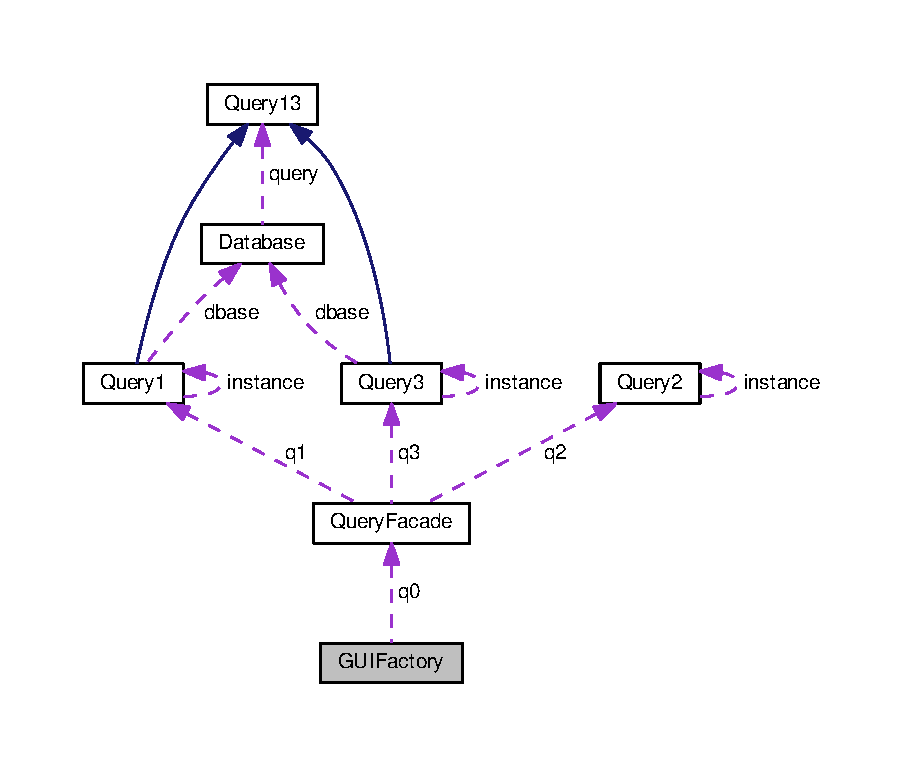
\includegraphics[width=350pt]{classGUIFactory__coll__graph}
\end{center}
\end{figure}
\subsection*{Public Member Functions}
\begin{DoxyCompactItemize}
\item 
\hyperlink{classGUIFactory_a133845e2346ee4986e09793e48a90241}{G\+U\+I\+Factory} (J\+Frame \hyperlink{classGUIFactory_afb70d82da7ea373c87a3cb8c2f6eb075}{main\+Frame}, J\+Combo\+Box$<$ String $>$ \hyperlink{classGUIFactory_a244f5c63e4a280528e2b08316a652287}{queries}, J\+Panel \hyperlink{classGUIFactory_a76d0958fe1b53efd8953c3744fc9db01}{side\+Panel}, J\+Panel \hyperlink{classGUIFactory_aa9d579163a66ea0c377f2dc87f9449dd}{display\+Panel}, \hyperlink{classQueryFacade}{Query\+Facade} q)
\item 
\hyperlink{classGUIQuery}{G\+U\+I\+Query} \hyperlink{classGUIFactory_a2b891d0369711430ae1d172f15b78317}{get\+Query} (String query\+Name)
\end{DoxyCompactItemize}
\subsection*{Private Attributes}
\begin{DoxyCompactItemize}
\item 
J\+Frame \hyperlink{classGUIFactory_afb70d82da7ea373c87a3cb8c2f6eb075}{main\+Frame}
\item 
J\+Panel \hyperlink{classGUIFactory_a76d0958fe1b53efd8953c3744fc9db01}{side\+Panel}
\item 
J\+Panel \hyperlink{classGUIFactory_aa9d579163a66ea0c377f2dc87f9449dd}{display\+Panel}
\item 
J\+Combo\+Box$<$ String $>$ \hyperlink{classGUIFactory_a244f5c63e4a280528e2b08316a652287}{queries}
\item 
\hyperlink{classQueryFacade}{Query\+Facade} \hyperlink{classGUIFactory_a6f1a7d65f7a410b4a47ce24164e1d594}{q0} =null
\end{DoxyCompactItemize}


\subsection{Detailed Description}
\hyperlink{classGUIFactory}{G\+U\+I\+Factory} returns insatce according to type specified, i.\+e. implements Factory Design Pattern 

\subsection{Constructor \& Destructor Documentation}
\index{G\+U\+I\+Factory@{G\+U\+I\+Factory}!G\+U\+I\+Factory@{G\+U\+I\+Factory}}
\index{G\+U\+I\+Factory@{G\+U\+I\+Factory}!G\+U\+I\+Factory@{G\+U\+I\+Factory}}
\subsubsection[{\texorpdfstring{G\+U\+I\+Factory(\+J\+Frame main\+Frame, J\+Combo\+Box$<$ String $>$ queries, J\+Panel side\+Panel, J\+Panel display\+Panel, Query\+Facade q)}{GUIFactory(JFrame mainFrame, JComboBox< String > queries, JPanel sidePanel, JPanel displayPanel, QueryFacade q)}}]{\setlength{\rightskip}{0pt plus 5cm}G\+U\+I\+Factory.\+G\+U\+I\+Factory (
\begin{DoxyParamCaption}
\item[{J\+Frame}]{main\+Frame, }
\item[{J\+Combo\+Box$<$ String $>$}]{queries, }
\item[{J\+Panel}]{side\+Panel, }
\item[{J\+Panel}]{display\+Panel, }
\item[{{\bf Query\+Facade}}]{q}
\end{DoxyParamCaption}
)\hspace{0.3cm}{\ttfamily [inline]}}\hypertarget{classGUIFactory_a133845e2346ee4986e09793e48a90241}{}\label{classGUIFactory_a133845e2346ee4986e09793e48a90241}

\begin{DoxyCode}
30     \{
31         this.\hyperlink{classGUIFactory_afb70d82da7ea373c87a3cb8c2f6eb075}{mainFrame}=\hyperlink{classGUIFactory_afb70d82da7ea373c87a3cb8c2f6eb075}{mainFrame};
32         this.\hyperlink{classGUIFactory_a244f5c63e4a280528e2b08316a652287}{queries}=\hyperlink{classGUIFactory_a244f5c63e4a280528e2b08316a652287}{queries};
33         this.\hyperlink{classGUIFactory_a76d0958fe1b53efd8953c3744fc9db01}{sidePanel}=\hyperlink{classGUIFactory_a76d0958fe1b53efd8953c3744fc9db01}{sidePanel};
34         this.\hyperlink{classGUIFactory_aa9d579163a66ea0c377f2dc87f9449dd}{displayPanel}=\hyperlink{classGUIFactory_aa9d579163a66ea0c377f2dc87f9449dd}{displayPanel};
35         this.\hyperlink{classGUIFactory_a6f1a7d65f7a410b4a47ce24164e1d594}{q0}=q;
36     \}
\end{DoxyCode}


\subsection{Member Function Documentation}
\index{G\+U\+I\+Factory@{G\+U\+I\+Factory}!get\+Query@{get\+Query}}
\index{get\+Query@{get\+Query}!G\+U\+I\+Factory@{G\+U\+I\+Factory}}
\subsubsection[{\texorpdfstring{get\+Query(\+String query\+Name)}{getQuery(String queryName)}}]{\setlength{\rightskip}{0pt plus 5cm}{\bf G\+U\+I\+Query} G\+U\+I\+Factory.\+get\+Query (
\begin{DoxyParamCaption}
\item[{String}]{query\+Name}
\end{DoxyParamCaption}
)\hspace{0.3cm}{\ttfamily [inline]}}\hypertarget{classGUIFactory_a2b891d0369711430ae1d172f15b78317}{}\label{classGUIFactory_a2b891d0369711430ae1d172f15b78317}

\begin{DoxyCode}
39     \{
40         \textcolor{keywordflow}{if}(queryName==null)\{
41             \textcolor{keywordflow}{return} null;
42         \}
43         \textcolor{keywordflow}{else} \textcolor{keywordflow}{if}(queryName.equalsIgnoreCase(\textcolor{stringliteral}{"Query1"}))\{
44             \textcolor{keywordflow}{return} \textcolor{keyword}{new} \hyperlink{classGuiQuery1Control}{GuiQuery1Control}(\hyperlink{classGUIFactory_afb70d82da7ea373c87a3cb8c2f6eb075}{mainFrame},
      \hyperlink{classGUIFactory_a244f5c63e4a280528e2b08316a652287}{queries},\hyperlink{classGUIFactory_a76d0958fe1b53efd8953c3744fc9db01}{sidePanel},\hyperlink{classGUIFactory_aa9d579163a66ea0c377f2dc87f9449dd}{displayPanel},\hyperlink{classGUIFactory_a6f1a7d65f7a410b4a47ce24164e1d594}{q0});
45         \} \textcolor{keywordflow}{else} \textcolor{keywordflow}{if}(queryName.equalsIgnoreCase(\textcolor{stringliteral}{"Query2"}))\{
46             \textcolor{keywordflow}{return} \textcolor{keyword}{new} \hyperlink{classGuiQuery2}{GuiQuery2}(\hyperlink{classGUIFactory_afb70d82da7ea373c87a3cb8c2f6eb075}{mainFrame},\hyperlink{classGUIFactory_a244f5c63e4a280528e2b08316a652287}{queries},
      \hyperlink{classGUIFactory_a76d0958fe1b53efd8953c3744fc9db01}{sidePanel},\hyperlink{classGUIFactory_aa9d579163a66ea0c377f2dc87f9449dd}{displayPanel},\hyperlink{classGUIFactory_a6f1a7d65f7a410b4a47ce24164e1d594}{q0});
47         \} \textcolor{keywordflow}{else} \textcolor{keywordflow}{if}(queryName.equalsIgnoreCase(\textcolor{stringliteral}{"Query3"}))\{
48             \textcolor{keywordflow}{return} \textcolor{keyword}{new} \hyperlink{classGuiQuery3}{GuiQuery3}(\hyperlink{classGUIFactory_afb70d82da7ea373c87a3cb8c2f6eb075}{mainFrame},\hyperlink{classGUIFactory_a244f5c63e4a280528e2b08316a652287}{queries},
      \hyperlink{classGUIFactory_a76d0958fe1b53efd8953c3744fc9db01}{sidePanel},\hyperlink{classGUIFactory_aa9d579163a66ea0c377f2dc87f9449dd}{displayPanel},\hyperlink{classGUIFactory_a6f1a7d65f7a410b4a47ce24164e1d594}{q0});
49         \}
50         \textcolor{keywordflow}{return} null;
51     \}
\end{DoxyCode}


\subsection{Member Data Documentation}
\index{G\+U\+I\+Factory@{G\+U\+I\+Factory}!display\+Panel@{display\+Panel}}
\index{display\+Panel@{display\+Panel}!G\+U\+I\+Factory@{G\+U\+I\+Factory}}
\subsubsection[{\texorpdfstring{display\+Panel}{displayPanel}}]{\setlength{\rightskip}{0pt plus 5cm}J\+Panel G\+U\+I\+Factory.\+display\+Panel\hspace{0.3cm}{\ttfamily [private]}}\hypertarget{classGUIFactory_aa9d579163a66ea0c377f2dc87f9449dd}{}\label{classGUIFactory_aa9d579163a66ea0c377f2dc87f9449dd}
\index{G\+U\+I\+Factory@{G\+U\+I\+Factory}!main\+Frame@{main\+Frame}}
\index{main\+Frame@{main\+Frame}!G\+U\+I\+Factory@{G\+U\+I\+Factory}}
\subsubsection[{\texorpdfstring{main\+Frame}{mainFrame}}]{\setlength{\rightskip}{0pt plus 5cm}J\+Frame G\+U\+I\+Factory.\+main\+Frame\hspace{0.3cm}{\ttfamily [private]}}\hypertarget{classGUIFactory_afb70d82da7ea373c87a3cb8c2f6eb075}{}\label{classGUIFactory_afb70d82da7ea373c87a3cb8c2f6eb075}
\index{G\+U\+I\+Factory@{G\+U\+I\+Factory}!q0@{q0}}
\index{q0@{q0}!G\+U\+I\+Factory@{G\+U\+I\+Factory}}
\subsubsection[{\texorpdfstring{q0}{q0}}]{\setlength{\rightskip}{0pt plus 5cm}{\bf Query\+Facade} G\+U\+I\+Factory.\+q0 =null\hspace{0.3cm}{\ttfamily [private]}}\hypertarget{classGUIFactory_a6f1a7d65f7a410b4a47ce24164e1d594}{}\label{classGUIFactory_a6f1a7d65f7a410b4a47ce24164e1d594}
\index{G\+U\+I\+Factory@{G\+U\+I\+Factory}!queries@{queries}}
\index{queries@{queries}!G\+U\+I\+Factory@{G\+U\+I\+Factory}}
\subsubsection[{\texorpdfstring{queries}{queries}}]{\setlength{\rightskip}{0pt plus 5cm}J\+Combo\+Box$<$String$>$ G\+U\+I\+Factory.\+queries\hspace{0.3cm}{\ttfamily [private]}}\hypertarget{classGUIFactory_a244f5c63e4a280528e2b08316a652287}{}\label{classGUIFactory_a244f5c63e4a280528e2b08316a652287}
\index{G\+U\+I\+Factory@{G\+U\+I\+Factory}!side\+Panel@{side\+Panel}}
\index{side\+Panel@{side\+Panel}!G\+U\+I\+Factory@{G\+U\+I\+Factory}}
\subsubsection[{\texorpdfstring{side\+Panel}{sidePanel}}]{\setlength{\rightskip}{0pt plus 5cm}J\+Panel G\+U\+I\+Factory.\+side\+Panel\hspace{0.3cm}{\ttfamily [private]}}\hypertarget{classGUIFactory_a76d0958fe1b53efd8953c3744fc9db01}{}\label{classGUIFactory_a76d0958fe1b53efd8953c3744fc9db01}


The documentation for this class was generated from the following file\+:\begin{DoxyCompactItemize}
\item 
\hyperlink{GUIFactory_8java}{G\+U\+I\+Factory.\+java}\end{DoxyCompactItemize}

\hypertarget{classGuiLoading}{}\section{Gui\+Loading Class Reference}
\label{classGuiLoading}\index{Gui\+Loading@{Gui\+Loading}}
\subsection*{Public Member Functions}
\begin{DoxyCompactItemize}
\item 
\hyperlink{classGuiLoading_a21afd225a3bb5a8e7542e662d39ea194}{Gui\+Loading} ()
\item 
void \hyperlink{classGuiLoading_aa13c96669e7ef681bfeae1a5b2dfab85}{start} ()
\item 
void \hyperlink{classGuiLoading_addd66da1f2d489192a2afdc66abef566}{stop} ()
\end{DoxyCompactItemize}
\subsection*{Private Attributes}
\begin{DoxyCompactItemize}
\item 
J\+Frame \hyperlink{classGuiLoading_a7790e84aa69edf129d802057d0420608}{loading\+Frame}
\item 
J\+Panel \hyperlink{classGuiLoading_ad7da2e974b1f70476fc92e8b3dc7e853}{loading\+Panel}
\item 
J\+Label \hyperlink{classGuiLoading_a885e7ee695236c2a7a4428658828b827}{loading\+Label}
\end{DoxyCompactItemize}


\subsection{Detailed Description}
Shows Loading 

\subsection{Constructor \& Destructor Documentation}
\index{Gui\+Loading@{Gui\+Loading}!Gui\+Loading@{Gui\+Loading}}
\index{Gui\+Loading@{Gui\+Loading}!Gui\+Loading@{Gui\+Loading}}
\subsubsection[{\texorpdfstring{Gui\+Loading()}{GuiLoading()}}]{\setlength{\rightskip}{0pt plus 5cm}Gui\+Loading.\+Gui\+Loading (
\begin{DoxyParamCaption}
{}
\end{DoxyParamCaption}
)\hspace{0.3cm}{\ttfamily [inline]}}\hypertarget{classGuiLoading_a21afd225a3bb5a8e7542e662d39ea194}{}\label{classGuiLoading_a21afd225a3bb5a8e7542e662d39ea194}

\begin{DoxyCode}
25     \{
26         System.out.println(\textcolor{stringliteral}{"Gui Loading"});
27         \hyperlink{classGuiLoading_a7790e84aa69edf129d802057d0420608}{loadingFrame}=\textcolor{keyword}{new} JFrame(\textcolor{stringliteral}{"Loading"});
28         \hyperlink{classGuiLoading_a7790e84aa69edf129d802057d0420608}{loadingFrame}.setSize(250,40); 
29         \hyperlink{classGuiLoading_a7790e84aa69edf129d802057d0420608}{loadingFrame}.setLocation(600,270);
30         \hyperlink{classGuiLoading_a7790e84aa69edf129d802057d0420608}{loadingFrame}.setResizable(\textcolor{keyword}{false});
31         \hyperlink{classGuiLoading_a7790e84aa69edf129d802057d0420608}{loadingFrame}.setLayout(\textcolor{keyword}{new} BoxLayout (\hyperlink{classGuiLoading_a7790e84aa69edf129d802057d0420608}{loadingFrame}.getContentPane(), 
      BoxLayout.Y\_AXIS));
32         \hyperlink{classGuiLoading_a7790e84aa69edf129d802057d0420608}{loadingFrame}.setDefaultCloseOperation(JFrame.EXIT\_ON\_CLOSE);
33         \hyperlink{classGuiLoading_ad7da2e974b1f70476fc92e8b3dc7e853}{loadingPanel}=\textcolor{keyword}{new} JPanel();
34         \hyperlink{classGuiLoading_a885e7ee695236c2a7a4428658828b827}{loadingLabel}=\textcolor{keyword}{new} JLabel(\textcolor{stringliteral}{"<html><b>Loading... Please Wait</b></html>"},JLabel.CENTER);
35         \hyperlink{classGuiLoading_a885e7ee695236c2a7a4428658828b827}{loadingLabel}.setFont(\textcolor{keyword}{new} Font(\textcolor{stringliteral}{"Calibri"}, Font.PLAIN, 15));
36         \hyperlink{classGuiLoading_a885e7ee695236c2a7a4428658828b827}{loadingLabel}.setAlignmentX(Component.CENTER\_ALIGNMENT);
37         \hyperlink{classGuiLoading_ad7da2e974b1f70476fc92e8b3dc7e853}{loadingPanel}.add(Box.createRigidArea(\textcolor{keyword}{new} Dimension(25,0)));
38         \hyperlink{classGuiLoading_ad7da2e974b1f70476fc92e8b3dc7e853}{loadingPanel}.add(\hyperlink{classGuiLoading_a885e7ee695236c2a7a4428658828b827}{loadingLabel});
39         \hyperlink{classGuiLoading_ad7da2e974b1f70476fc92e8b3dc7e853}{loadingPanel}.setVisible(\textcolor{keyword}{true});
40         \hyperlink{classGuiLoading_a7790e84aa69edf129d802057d0420608}{loadingFrame}.add(\hyperlink{classGuiLoading_ad7da2e974b1f70476fc92e8b3dc7e853}{loadingPanel});
41     \}
\end{DoxyCode}


\subsection{Member Function Documentation}
\index{Gui\+Loading@{Gui\+Loading}!start@{start}}
\index{start@{start}!Gui\+Loading@{Gui\+Loading}}
\subsubsection[{\texorpdfstring{start()}{start()}}]{\setlength{\rightskip}{0pt plus 5cm}void Gui\+Loading.\+start (
\begin{DoxyParamCaption}
{}
\end{DoxyParamCaption}
)\hspace{0.3cm}{\ttfamily [inline]}}\hypertarget{classGuiLoading_aa13c96669e7ef681bfeae1a5b2dfab85}{}\label{classGuiLoading_aa13c96669e7ef681bfeae1a5b2dfab85}

\begin{DoxyCode}
44     \{
45         \hyperlink{classGuiLoading_a7790e84aa69edf129d802057d0420608}{loadingFrame}.setVisible(\textcolor{keyword}{true});
46     \}   
\end{DoxyCode}
\index{Gui\+Loading@{Gui\+Loading}!stop@{stop}}
\index{stop@{stop}!Gui\+Loading@{Gui\+Loading}}
\subsubsection[{\texorpdfstring{stop()}{stop()}}]{\setlength{\rightskip}{0pt plus 5cm}void Gui\+Loading.\+stop (
\begin{DoxyParamCaption}
{}
\end{DoxyParamCaption}
)\hspace{0.3cm}{\ttfamily [inline]}}\hypertarget{classGuiLoading_addd66da1f2d489192a2afdc66abef566}{}\label{classGuiLoading_addd66da1f2d489192a2afdc66abef566}

\begin{DoxyCode}
49     \{
50         \hyperlink{classGuiLoading_a7790e84aa69edf129d802057d0420608}{loadingFrame}.setVisible(\textcolor{keyword}{false});
51     \}
\end{DoxyCode}


\subsection{Member Data Documentation}
\index{Gui\+Loading@{Gui\+Loading}!loading\+Frame@{loading\+Frame}}
\index{loading\+Frame@{loading\+Frame}!Gui\+Loading@{Gui\+Loading}}
\subsubsection[{\texorpdfstring{loading\+Frame}{loadingFrame}}]{\setlength{\rightskip}{0pt plus 5cm}J\+Frame Gui\+Loading.\+loading\+Frame\hspace{0.3cm}{\ttfamily [private]}}\hypertarget{classGuiLoading_a7790e84aa69edf129d802057d0420608}{}\label{classGuiLoading_a7790e84aa69edf129d802057d0420608}
\index{Gui\+Loading@{Gui\+Loading}!loading\+Label@{loading\+Label}}
\index{loading\+Label@{loading\+Label}!Gui\+Loading@{Gui\+Loading}}
\subsubsection[{\texorpdfstring{loading\+Label}{loadingLabel}}]{\setlength{\rightskip}{0pt plus 5cm}J\+Label Gui\+Loading.\+loading\+Label\hspace{0.3cm}{\ttfamily [private]}}\hypertarget{classGuiLoading_a885e7ee695236c2a7a4428658828b827}{}\label{classGuiLoading_a885e7ee695236c2a7a4428658828b827}
\index{Gui\+Loading@{Gui\+Loading}!loading\+Panel@{loading\+Panel}}
\index{loading\+Panel@{loading\+Panel}!Gui\+Loading@{Gui\+Loading}}
\subsubsection[{\texorpdfstring{loading\+Panel}{loadingPanel}}]{\setlength{\rightskip}{0pt plus 5cm}J\+Panel Gui\+Loading.\+loading\+Panel\hspace{0.3cm}{\ttfamily [private]}}\hypertarget{classGuiLoading_ad7da2e974b1f70476fc92e8b3dc7e853}{}\label{classGuiLoading_ad7da2e974b1f70476fc92e8b3dc7e853}


The documentation for this class was generated from the following file\+:\begin{DoxyCompactItemize}
\item 
\hyperlink{GuiLoading_8java}{Gui\+Loading.\+java}\end{DoxyCompactItemize}

\hypertarget{classGUIQuery}{}\section{G\+U\+I\+Query Class Reference}
\label{classGUIQuery}\index{G\+U\+I\+Query@{G\+U\+I\+Query}}


Inheritance diagram for G\+U\+I\+Query\+:\nopagebreak
\begin{figure}[H]
\begin{center}
\leavevmode
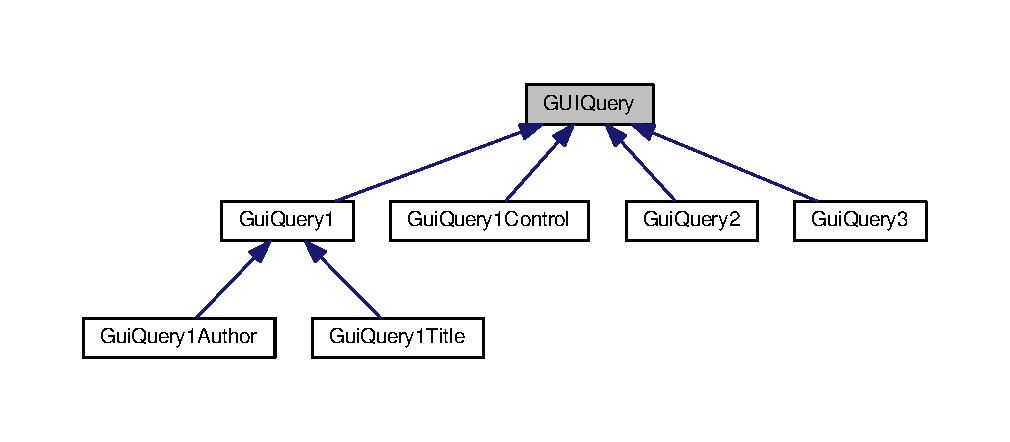
\includegraphics[width=350pt]{classGUIQuery__inherit__graph}
\end{center}
\end{figure}


Collaboration diagram for G\+U\+I\+Query\+:\nopagebreak
\begin{figure}[H]
\begin{center}
\leavevmode
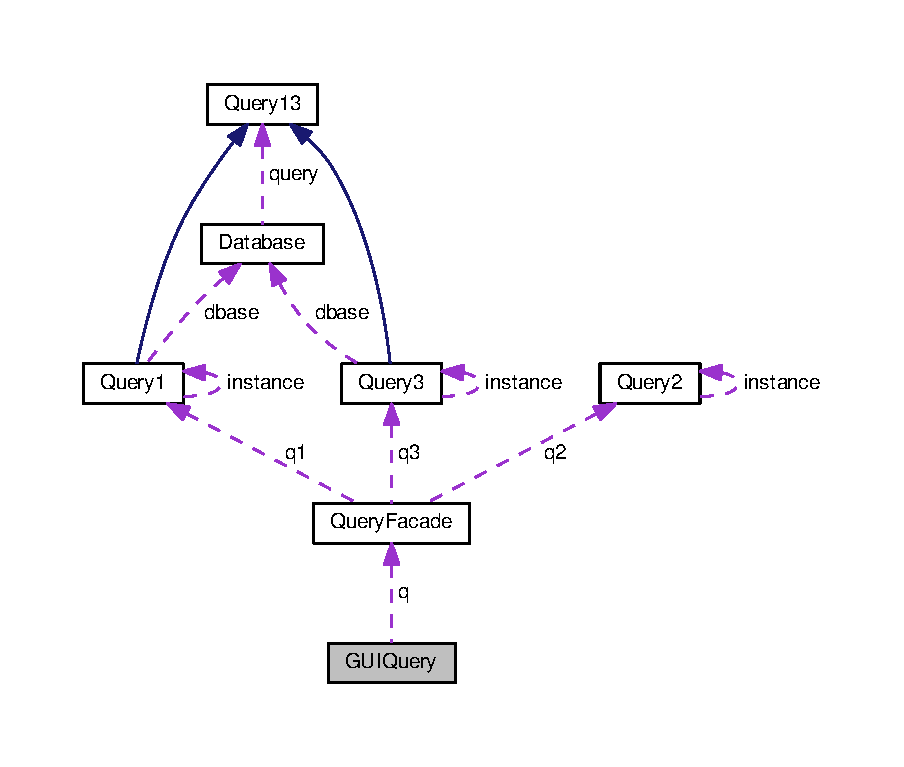
\includegraphics[width=350pt]{classGUIQuery__coll__graph}
\end{center}
\end{figure}
\subsection*{Public Member Functions}
\begin{DoxyCompactItemize}
\item 
abstract void \hyperlink{classGUIQuery_ac2ad3b1e3b09ddc71b4df76397786553}{init\+Query} ()
\item 
abstract void \hyperlink{classGUIQuery_a5ab63c960b5a562e5daa4be87dec89e3}{set\+Query} ()
\item 
final void \hyperlink{classGUIQuery_acc9553514ecac053151c7580b83dec21}{start} ()
\item 
boolean \hyperlink{classGUIQuery_a2ffddedac70e763f8d4bfc6d24d9a0db}{is\+Integer} (String s)
\end{DoxyCompactItemize}
\subsection*{Protected Attributes}
\begin{DoxyCompactItemize}
\item 
J\+Frame \hyperlink{classGUIQuery_aba988b5bec899d53480a472de7b87dfa}{main\+Frame}
\item 
J\+Panel \hyperlink{classGUIQuery_a37a678b81901083072a73283d7acf52f}{upper\+Panel}
\item 
J\+Panel \hyperlink{classGUIQuery_a70e233b1f14874166b7707edebe825d2}{side\+Panel}
\item 
J\+Panel \hyperlink{classGUIQuery_a8b4dbf257e0859c597591f072349b75c}{display\+Panel}
\item 
J\+Combo\+Box$<$ String $>$ \hyperlink{classGUIQuery_a0db8bd960b4512cadf9aa40642934680}{queries}
\item 
J\+Button \hyperlink{classGUIQuery_a6580b15e365bc754c1a5ccdd2d58a4bb}{submit}
\item 
\hyperlink{classQueryFacade}{Query\+Facade} \hyperlink{classGUIQuery_a2a20445d749185552014142b78f3e071}{q} =null
\end{DoxyCompactItemize}


\subsection{Detailed Description}
Provides Template Design Pattern 

\subsection{Member Function Documentation}
\index{G\+U\+I\+Query@{G\+U\+I\+Query}!init\+Query@{init\+Query}}
\index{init\+Query@{init\+Query}!G\+U\+I\+Query@{G\+U\+I\+Query}}
\subsubsection[{\texorpdfstring{init\+Query()}{initQuery()}}]{\setlength{\rightskip}{0pt plus 5cm}abstract void G\+U\+I\+Query.\+init\+Query (
\begin{DoxyParamCaption}
{}
\end{DoxyParamCaption}
)\hspace{0.3cm}{\ttfamily [abstract]}}\hypertarget{classGUIQuery_ac2ad3b1e3b09ddc71b4df76397786553}{}\label{classGUIQuery_ac2ad3b1e3b09ddc71b4df76397786553}
\index{G\+U\+I\+Query@{G\+U\+I\+Query}!is\+Integer@{is\+Integer}}
\index{is\+Integer@{is\+Integer}!G\+U\+I\+Query@{G\+U\+I\+Query}}
\subsubsection[{\texorpdfstring{is\+Integer(\+String s)}{isInteger(String s)}}]{\setlength{\rightskip}{0pt plus 5cm}boolean G\+U\+I\+Query.\+is\+Integer (
\begin{DoxyParamCaption}
\item[{String}]{s}
\end{DoxyParamCaption}
)\hspace{0.3cm}{\ttfamily [inline]}}\hypertarget{classGUIQuery_a2ffddedac70e763f8d4bfc6d24d9a0db}{}\label{classGUIQuery_a2ffddedac70e763f8d4bfc6d24d9a0db}

\begin{DoxyCode}
36                                        \{
37       \textcolor{keywordtype}{boolean} isValidInteger = \textcolor{keyword}{false};
38       \textcolor{keywordflow}{try}
39       \{
40          Integer.parseInt(s);
41          isValidInteger = \textcolor{keyword}{true};
42       \}
43       \textcolor{keywordflow}{catch} (NumberFormatException ex)
44       \{\}
45       \textcolor{keywordflow}{return} isValidInteger;
46    \}
\end{DoxyCode}
\index{G\+U\+I\+Query@{G\+U\+I\+Query}!set\+Query@{set\+Query}}
\index{set\+Query@{set\+Query}!G\+U\+I\+Query@{G\+U\+I\+Query}}
\subsubsection[{\texorpdfstring{set\+Query()}{setQuery()}}]{\setlength{\rightskip}{0pt plus 5cm}abstract void G\+U\+I\+Query.\+set\+Query (
\begin{DoxyParamCaption}
{}
\end{DoxyParamCaption}
)\hspace{0.3cm}{\ttfamily [abstract]}}\hypertarget{classGUIQuery_a5ab63c960b5a562e5daa4be87dec89e3}{}\label{classGUIQuery_a5ab63c960b5a562e5daa4be87dec89e3}
\index{G\+U\+I\+Query@{G\+U\+I\+Query}!start@{start}}
\index{start@{start}!G\+U\+I\+Query@{G\+U\+I\+Query}}
\subsubsection[{\texorpdfstring{start()}{start()}}]{\setlength{\rightskip}{0pt plus 5cm}final void G\+U\+I\+Query.\+start (
\begin{DoxyParamCaption}
{}
\end{DoxyParamCaption}
)\hspace{0.3cm}{\ttfamily [inline]}}\hypertarget{classGUIQuery_acc9553514ecac053151c7580b83dec21}{}\label{classGUIQuery_acc9553514ecac053151c7580b83dec21}

\begin{DoxyCode}
31     \{
32         \hyperlink{classGUIQuery_ac2ad3b1e3b09ddc71b4df76397786553}{initQuery}();
33         \hyperlink{classGUIQuery_a5ab63c960b5a562e5daa4be87dec89e3}{setQuery}();
34     \}
\end{DoxyCode}


\subsection{Member Data Documentation}
\index{G\+U\+I\+Query@{G\+U\+I\+Query}!display\+Panel@{display\+Panel}}
\index{display\+Panel@{display\+Panel}!G\+U\+I\+Query@{G\+U\+I\+Query}}
\subsubsection[{\texorpdfstring{display\+Panel}{displayPanel}}]{\setlength{\rightskip}{0pt plus 5cm}J\+Panel G\+U\+I\+Query.\+display\+Panel\hspace{0.3cm}{\ttfamily [protected]}}\hypertarget{classGUIQuery_a8b4dbf257e0859c597591f072349b75c}{}\label{classGUIQuery_a8b4dbf257e0859c597591f072349b75c}
\index{G\+U\+I\+Query@{G\+U\+I\+Query}!main\+Frame@{main\+Frame}}
\index{main\+Frame@{main\+Frame}!G\+U\+I\+Query@{G\+U\+I\+Query}}
\subsubsection[{\texorpdfstring{main\+Frame}{mainFrame}}]{\setlength{\rightskip}{0pt plus 5cm}J\+Frame G\+U\+I\+Query.\+main\+Frame\hspace{0.3cm}{\ttfamily [protected]}}\hypertarget{classGUIQuery_aba988b5bec899d53480a472de7b87dfa}{}\label{classGUIQuery_aba988b5bec899d53480a472de7b87dfa}
\index{G\+U\+I\+Query@{G\+U\+I\+Query}!q@{q}}
\index{q@{q}!G\+U\+I\+Query@{G\+U\+I\+Query}}
\subsubsection[{\texorpdfstring{q}{q}}]{\setlength{\rightskip}{0pt plus 5cm}{\bf Query\+Facade} G\+U\+I\+Query.\+q =null\hspace{0.3cm}{\ttfamily [protected]}}\hypertarget{classGUIQuery_a2a20445d749185552014142b78f3e071}{}\label{classGUIQuery_a2a20445d749185552014142b78f3e071}
\index{G\+U\+I\+Query@{G\+U\+I\+Query}!queries@{queries}}
\index{queries@{queries}!G\+U\+I\+Query@{G\+U\+I\+Query}}
\subsubsection[{\texorpdfstring{queries}{queries}}]{\setlength{\rightskip}{0pt plus 5cm}J\+Combo\+Box$<$String$>$ G\+U\+I\+Query.\+queries\hspace{0.3cm}{\ttfamily [protected]}}\hypertarget{classGUIQuery_a0db8bd960b4512cadf9aa40642934680}{}\label{classGUIQuery_a0db8bd960b4512cadf9aa40642934680}
\index{G\+U\+I\+Query@{G\+U\+I\+Query}!side\+Panel@{side\+Panel}}
\index{side\+Panel@{side\+Panel}!G\+U\+I\+Query@{G\+U\+I\+Query}}
\subsubsection[{\texorpdfstring{side\+Panel}{sidePanel}}]{\setlength{\rightskip}{0pt plus 5cm}J\+Panel G\+U\+I\+Query.\+side\+Panel\hspace{0.3cm}{\ttfamily [protected]}}\hypertarget{classGUIQuery_a70e233b1f14874166b7707edebe825d2}{}\label{classGUIQuery_a70e233b1f14874166b7707edebe825d2}
\index{G\+U\+I\+Query@{G\+U\+I\+Query}!submit@{submit}}
\index{submit@{submit}!G\+U\+I\+Query@{G\+U\+I\+Query}}
\subsubsection[{\texorpdfstring{submit}{submit}}]{\setlength{\rightskip}{0pt plus 5cm}J\+Button G\+U\+I\+Query.\+submit\hspace{0.3cm}{\ttfamily [protected]}}\hypertarget{classGUIQuery_a6580b15e365bc754c1a5ccdd2d58a4bb}{}\label{classGUIQuery_a6580b15e365bc754c1a5ccdd2d58a4bb}
\index{G\+U\+I\+Query@{G\+U\+I\+Query}!upper\+Panel@{upper\+Panel}}
\index{upper\+Panel@{upper\+Panel}!G\+U\+I\+Query@{G\+U\+I\+Query}}
\subsubsection[{\texorpdfstring{upper\+Panel}{upperPanel}}]{\setlength{\rightskip}{0pt plus 5cm}J\+Panel G\+U\+I\+Query.\+upper\+Panel\hspace{0.3cm}{\ttfamily [protected]}}\hypertarget{classGUIQuery_a37a678b81901083072a73283d7acf52f}{}\label{classGUIQuery_a37a678b81901083072a73283d7acf52f}


The documentation for this class was generated from the following file\+:\begin{DoxyCompactItemize}
\item 
\hyperlink{GUIQuery_8java}{G\+U\+I\+Query.\+java}\end{DoxyCompactItemize}

\hypertarget{classGuiQuery1}{}\section{Gui\+Query1 Class Reference}
\label{classGuiQuery1}\index{Gui\+Query1@{Gui\+Query1}}


Inheritance diagram for Gui\+Query1\+:\nopagebreak
\begin{figure}[H]
\begin{center}
\leavevmode
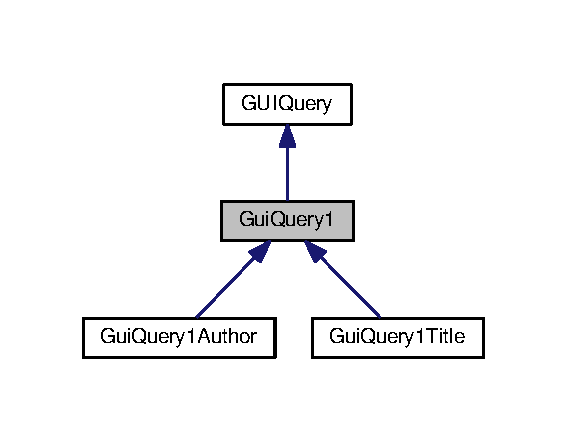
\includegraphics[width=272pt]{classGuiQuery1__inherit__graph}
\end{center}
\end{figure}


Collaboration diagram for Gui\+Query1\+:\nopagebreak
\begin{figure}[H]
\begin{center}
\leavevmode
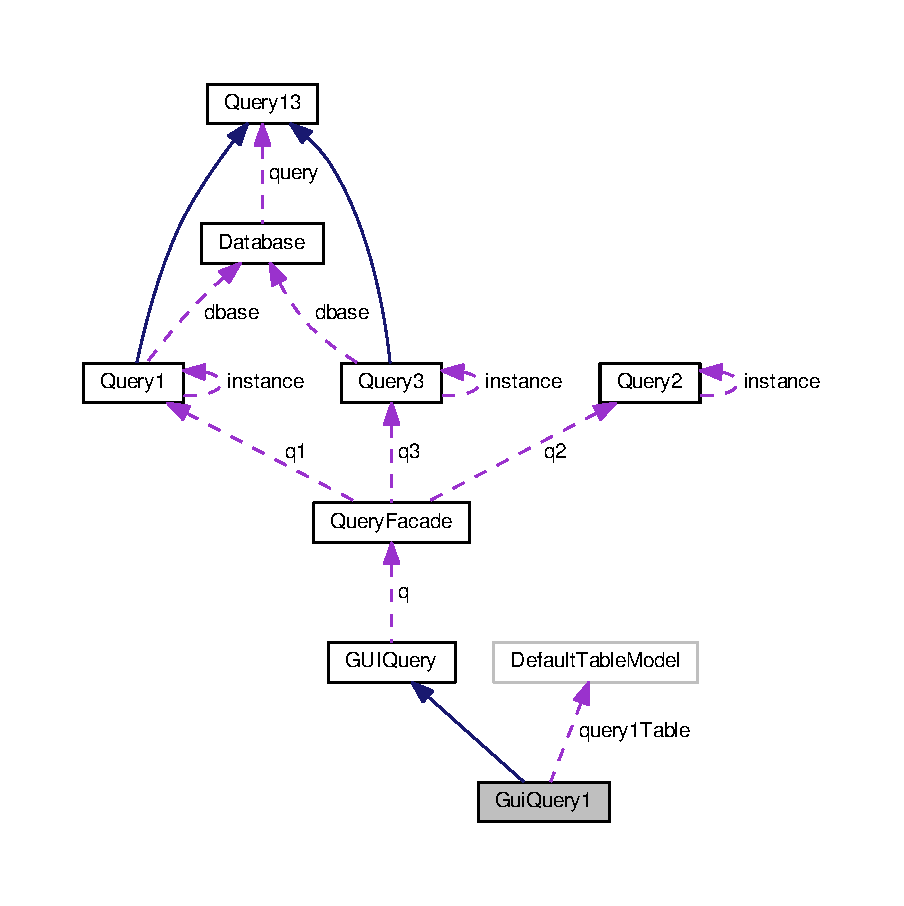
\includegraphics[width=350pt]{classGuiQuery1__coll__graph}
\end{center}
\end{figure}
\subsection*{Public Member Functions}
\begin{DoxyCompactItemize}
\item 
\hyperlink{classGuiQuery1_a8d4175f68c1145511607f64c24587f1c}{Gui\+Query1} (J\+Frame \hyperlink{classGUIQuery_aba988b5bec899d53480a472de7b87dfa}{main\+Frame}, J\+Combo\+Box$<$ String $>$ \hyperlink{classGUIQuery_a0db8bd960b4512cadf9aa40642934680}{queries}, J\+Panel \hyperlink{classGUIQuery_a70e233b1f14874166b7707edebe825d2}{side\+Panel}, J\+Panel \hyperlink{classGUIQuery_a8b4dbf257e0859c597591f072349b75c}{display\+Panel}, \hyperlink{classQueryFacade}{Query\+Facade} q1, J\+Combo\+Box$<$ String $>$ \hyperlink{classGuiQuery1_a021ae2f4fa2ec342496af6ac434995f4}{search\+By})
\item 
void \hyperlink{classGuiQuery1_a6159d6fe4b28473a93305c7f07405de9}{init\+Query} ()
\item 
void \hyperlink{classGuiQuery1_abe08121cbcebdc066aaec8400bc73cc7}{change} (int i)
\item 
void \hyperlink{classGuiQuery1_aa78daa5f76f85f27e3bbde79748bd34d}{change\+Mode} (int i)
\item 
void \hyperlink{classGuiQuery1_a9b24d0be68c88545f87a5a5bfb676cb2}{set\+Query} ()
\end{DoxyCompactItemize}
\subsection*{Protected Attributes}
\begin{DoxyCompactItemize}
\item 
Default\+Table\+Model \hyperlink{classGuiQuery1_ab9463b1a4a59d6c13bc04963b2b3f2c2}{query1\+Table} = new Default\+Table\+Model()
\item 
J\+Table \hyperlink{classGuiQuery1_aa23b7fb33949ccf74ca5be46e85eb578}{display\+Table} = new J\+Table(\hyperlink{classGuiQuery1_ab9463b1a4a59d6c13bc04963b2b3f2c2}{query1\+Table})
\item 
J\+Scroll\+Pane \hyperlink{classGuiQuery1_aaa4f69c2faaffb0b451f1fa5bfebc4d3}{disp\+Table} = new J\+Scroll\+Pane(\hyperlink{classGuiQuery1_aa23b7fb33949ccf74ca5be46e85eb578}{display\+Table})
\item 
J\+Button \hyperlink{classGuiQuery1_a0ef1bc892139ef28ea2e6c464f78e881}{next} = new J\+Button(\char`\"{}N\+E\+XT\char`\"{})
\item 
J\+Button \hyperlink{classGuiQuery1_a2b884d6a7f21de2efe0640e21fe6aadd}{back} = new J\+Button(\char`\"{}B\+A\+CK\char`\"{})
\item 
J\+Combo\+Box$<$ String $>$ \hyperlink{classGuiQuery1_a021ae2f4fa2ec342496af6ac434995f4}{search\+By} = new J\+Combo\+Box$<$String$>$()
\item 
J\+Label \hyperlink{classGuiQuery1_a31e28191d4f156f0367a7dac29b65836}{title1} = new J\+Label(\char`\"{}Name / Title tags\char`\"{})
\item 
J\+Label \hyperlink{classGuiQuery1_ad120c79c1fe5e4b3ce09960942924c0d}{title2} = new J\+Label(\char`\"{}Since Year\char`\"{})
\item 
J\+Label \hyperlink{classGuiQuery1_a8e28412d9118fc61abde587c3bf7574f}{title3} = new J\+Label(\char`\"{}Custom Range\char`\"{})
\item 
J\+Label \hyperlink{classGuiQuery1_a80ba7c84c9af8294566e3c1f1787c4a3}{result} = new J\+Label()
\item 
J\+Label \hyperlink{classGuiQuery1_a382ff58e8c0283a69f6d88249b1fe496}{warning} = new J\+Label(\char`\"{} \char`\"{})
\item 
J\+Label \hyperlink{classGuiQuery1_a40b4913205157f6e39c46956654a11f2}{dash} = new J\+Label(\char`\"{}-\/\char`\"{})
\item 
J\+Text\+Field \hyperlink{classGuiQuery1_aeebb26c926dc7045d9bd99dd3568eb45}{title} =new J\+Text\+Field()
\item 
J\+Text\+Field \hyperlink{classGuiQuery1_a8659841dac2a5dcf9b367a7b19a19a52}{year1} =new J\+Text\+Field()
\item 
J\+Text\+Field \hyperlink{classGuiQuery1_a012c8e122c0a83d0af4ca51d03932c37}{year2} =new J\+Text\+Field()
\item 
J\+Text\+Field \hyperlink{classGuiQuery1_ac74d62ae05c068aaa998c52121501978}{year3} =new J\+Text\+Field()
\item 
int \hyperlink{classGuiQuery1_a46ee2c343bc43a1c9a6278d9520b31f2}{flag} =0
\item 
J\+Label \hyperlink{classGuiQuery1_a515a1ac46f1362d811dd6e0c27d842fc}{total\+Results} = new J\+Label(\char`\"{} \char`\"{})
\end{DoxyCompactItemize}


\subsection{Detailed Description}
Creates the \hyperlink{classGUI}{G\+UI} needed for supporting \hyperlink{classQuery1}{Query1} 

\subsection{Constructor \& Destructor Documentation}
\index{Gui\+Query1@{Gui\+Query1}!Gui\+Query1@{Gui\+Query1}}
\index{Gui\+Query1@{Gui\+Query1}!Gui\+Query1@{Gui\+Query1}}
\subsubsection[{\texorpdfstring{Gui\+Query1(\+J\+Frame main\+Frame, J\+Combo\+Box$<$ String $>$ queries, J\+Panel side\+Panel, J\+Panel display\+Panel, Query\+Facade q1, J\+Combo\+Box$<$ String $>$ search\+By)}{GuiQuery1(JFrame mainFrame, JComboBox< String > queries, JPanel sidePanel, JPanel displayPanel, QueryFacade q1, JComboBox< String > searchBy)}}]{\setlength{\rightskip}{0pt plus 5cm}Gui\+Query1.\+Gui\+Query1 (
\begin{DoxyParamCaption}
\item[{J\+Frame}]{main\+Frame, }
\item[{J\+Combo\+Box$<$ String $>$}]{queries, }
\item[{J\+Panel}]{side\+Panel, }
\item[{J\+Panel}]{display\+Panel, }
\item[{{\bf Query\+Facade}}]{q1, }
\item[{J\+Combo\+Box$<$ String $>$}]{search\+By}
\end{DoxyParamCaption}
)\hspace{0.3cm}{\ttfamily [inline]}}\hypertarget{classGuiQuery1_a8d4175f68c1145511607f64c24587f1c}{}\label{classGuiQuery1_a8d4175f68c1145511607f64c24587f1c}

\begin{DoxyCode}
40     \{
41         this.\hyperlink{classGUIQuery_aba988b5bec899d53480a472de7b87dfa}{mainFrame}=\hyperlink{classGUIQuery_aba988b5bec899d53480a472de7b87dfa}{mainFrame};
42         this.\hyperlink{classGUIQuery_a0db8bd960b4512cadf9aa40642934680}{queries}=\hyperlink{classGUIQuery_a0db8bd960b4512cadf9aa40642934680}{queries};
43         this.\hyperlink{classGUIQuery_a70e233b1f14874166b7707edebe825d2}{sidePanel}=\hyperlink{classGUIQuery_a70e233b1f14874166b7707edebe825d2}{sidePanel};
44         this.\hyperlink{classGUIQuery_a8b4dbf257e0859c597591f072349b75c}{displayPanel}=\hyperlink{classGUIQuery_a8b4dbf257e0859c597591f072349b75c}{displayPanel};
45         this.\hyperlink{classGuiQuery1_a021ae2f4fa2ec342496af6ac434995f4}{searchBy}=\hyperlink{classGuiQuery1_a021ae2f4fa2ec342496af6ac434995f4}{searchBy};
46         this.\hyperlink{classGUIQuery_a2a20445d749185552014142b78f3e071}{q}=q1;
47     \}
\end{DoxyCode}


\subsection{Member Function Documentation}
\index{Gui\+Query1@{Gui\+Query1}!change@{change}}
\index{change@{change}!Gui\+Query1@{Gui\+Query1}}
\subsubsection[{\texorpdfstring{change(int i)}{change(int i)}}]{\setlength{\rightskip}{0pt plus 5cm}void Gui\+Query1.\+change (
\begin{DoxyParamCaption}
\item[{int}]{i}
\end{DoxyParamCaption}
)\hspace{0.3cm}{\ttfamily [inline]}}\hypertarget{classGuiQuery1_abe08121cbcebdc066aaec8400bc73cc7}{}\label{classGuiQuery1_abe08121cbcebdc066aaec8400bc73cc7}

\begin{DoxyCode}
101     \{
102         \hyperlink{classGuiQuery1_a46ee2c343bc43a1c9a6278d9520b31f2}{flag}=i;
103     \}
\end{DoxyCode}
\index{Gui\+Query1@{Gui\+Query1}!change\+Mode@{change\+Mode}}
\index{change\+Mode@{change\+Mode}!Gui\+Query1@{Gui\+Query1}}
\subsubsection[{\texorpdfstring{change\+Mode(int i)}{changeMode(int i)}}]{\setlength{\rightskip}{0pt plus 5cm}void Gui\+Query1.\+change\+Mode (
\begin{DoxyParamCaption}
\item[{int}]{i}
\end{DoxyParamCaption}
)\hspace{0.3cm}{\ttfamily [inline]}}\hypertarget{classGuiQuery1_aa78daa5f76f85f27e3bbde79748bd34d}{}\label{classGuiQuery1_aa78daa5f76f85f27e3bbde79748bd34d}

\begin{DoxyCode}
105     \{
106         flag2=i;
107     \}
\end{DoxyCode}
\index{Gui\+Query1@{Gui\+Query1}!init\+Query@{init\+Query}}
\index{init\+Query@{init\+Query}!Gui\+Query1@{Gui\+Query1}}
\subsubsection[{\texorpdfstring{init\+Query()}{initQuery()}}]{\setlength{\rightskip}{0pt plus 5cm}void Gui\+Query1.\+init\+Query (
\begin{DoxyParamCaption}
{}
\end{DoxyParamCaption}
)\hspace{0.3cm}{\ttfamily [inline]}}\hypertarget{classGuiQuery1_a6159d6fe4b28473a93305c7f07405de9}{}\label{classGuiQuery1_a6159d6fe4b28473a93305c7f07405de9}

\begin{DoxyCode}
50     \{
51         \hyperlink{classGuiQuery1_aa23b7fb33949ccf74ca5be46e85eb578}{displayTable}.setDefaultEditor(Object.class, null);
52         \hyperlink{classGuiQuery1_aaa4f69c2faaffb0b451f1fa5bfebc4d3}{dispTable}.setBounds(20,5,910,390);
53         \hyperlink{classGuiQuery1_ab9463b1a4a59d6c13bc04963b2b3f2c2}{query1Table}.addColumn(\textcolor{stringliteral}{"S.No."});
54         \hyperlink{classGuiQuery1_ab9463b1a4a59d6c13bc04963b2b3f2c2}{query1Table}.addColumn(\textcolor{stringliteral}{"Authors"});
55         \hyperlink{classGuiQuery1_ab9463b1a4a59d6c13bc04963b2b3f2c2}{query1Table}.addColumn(\textcolor{stringliteral}{"Title"});
56         \hyperlink{classGuiQuery1_ab9463b1a4a59d6c13bc04963b2b3f2c2}{query1Table}.addColumn(\textcolor{stringliteral}{"Pages"});
57         \hyperlink{classGuiQuery1_ab9463b1a4a59d6c13bc04963b2b3f2c2}{query1Table}.addColumn(\textcolor{stringliteral}{"Year"});
58         \hyperlink{classGuiQuery1_ab9463b1a4a59d6c13bc04963b2b3f2c2}{query1Table}.addColumn(\textcolor{stringliteral}{"Volume"});
59         \hyperlink{classGuiQuery1_ab9463b1a4a59d6c13bc04963b2b3f2c2}{query1Table}.addColumn(\textcolor{stringliteral}{"Journal/Booktitle"});
60         \hyperlink{classGuiQuery1_ab9463b1a4a59d6c13bc04963b2b3f2c2}{query1Table}.addColumn(\textcolor{stringliteral}{"Url"});
61         \hyperlink{classGuiQuery1_a0ef1bc892139ef28ea2e6c464f78e881}{next}.setBounds(840,395,80,40);
62         \hyperlink{classGuiQuery1_a0ef1bc892139ef28ea2e6c464f78e881}{next}.setBackground(Color.RED);
63         \hyperlink{classGuiQuery1_a0ef1bc892139ef28ea2e6c464f78e881}{next}.setFont(\textcolor{keyword}{new} Font(\textcolor{stringliteral}{"Calibri"}, Font.PLAIN, 10));
64         \hyperlink{classGuiQuery1_a2b884d6a7f21de2efe0640e21fe6aadd}{back}.setBounds(30,335,80,40);
65         \hyperlink{classGuiQuery1_a2b884d6a7f21de2efe0640e21fe6aadd}{back}.setBackground(Color.BLACK);
66         \hyperlink{classGuiQuery1_a2b884d6a7f21de2efe0640e21fe6aadd}{back}.setFont(\textcolor{keyword}{new} Font(\textcolor{stringliteral}{"Calibri"}, Font.PLAIN, 10));
67         \hyperlink{classGuiQuery1_a31e28191d4f156f0367a7dac29b65836}{title1}.setFont(\textcolor{keyword}{new} Font(\textcolor{stringliteral}{"Calibri"}, Font.PLAIN, 10));
68         \hyperlink{classGuiQuery1_ad120c79c1fe5e4b3ce09960942924c0d}{title2}.setFont(\textcolor{keyword}{new} Font(\textcolor{stringliteral}{"Calibri"}, Font.PLAIN, 10));
69         \hyperlink{classGuiQuery1_a8e28412d9118fc61abde587c3bf7574f}{title3}.setFont(\textcolor{keyword}{new} Font(\textcolor{stringliteral}{"Calibri"}, Font.PLAIN, 10));
70         \hyperlink{classGuiQuery1_a40b4913205157f6e39c46956654a11f2}{dash}.setFont(\textcolor{keyword}{new} Font(\textcolor{stringliteral}{"Calibri"}, Font.PLAIN, 10));  
71         \hyperlink{classGuiQuery1_a80ba7c84c9af8294566e3c1f1787c4a3}{result}.setFont(\textcolor{keyword}{new} Font(\textcolor{stringliteral}{"Calibri"}, Font.PLAIN, 15));
72         \hyperlink{classGuiQuery1_a382ff58e8c0283a69f6d88249b1fe496}{warning}.setFont(\textcolor{keyword}{new} Font(\textcolor{stringliteral}{"Calibri"}, Font.PLAIN, 12));
73         \hyperlink{classGuiQuery1_a382ff58e8c0283a69f6d88249b1fe496}{warning}.setForeground(Color.RED);
74         \hyperlink{classGuiQuery1_a31e28191d4f156f0367a7dac29b65836}{title1}.setBounds(30,90,100,20);
75         \hyperlink{classGuiQuery1_ad120c79c1fe5e4b3ce09960942924c0d}{title2}.setBounds(30,130,100,20);
76         \hyperlink{classGuiQuery1_a8e28412d9118fc61abde587c3bf7574f}{title3}.setBounds(30,155,100,20);
77         \hyperlink{classGuiQuery1_a40b4913205157f6e39c46956654a11f2}{dash}.setBounds(170,155,10,20);
78         \hyperlink{classGuiQuery1_a80ba7c84c9af8294566e3c1f1787c4a3}{result}.setBounds(50,120,350,50);
79         \hyperlink{classGuiQuery1_a382ff58e8c0283a69f6d88249b1fe496}{warning}.setBounds(30,340,190,20);
80         \hyperlink{classGuiQuery1_a515a1ac46f1362d811dd6e0c27d842fc}{totalResults}.setFont(\textcolor{keyword}{new} Font(\textcolor{stringliteral}{"Calibri"}, Font.PLAIN, 10));
81         \hyperlink{classGuiQuery1_a515a1ac46f1362d811dd6e0c27d842fc}{totalResults}.setBounds(515,395,120,30);
82         \hyperlink{classGuiQuery1_a8659841dac2a5dcf9b367a7b19a19a52}{year1}.setHorizontalAlignment(JTextField.CENTER);
83         \hyperlink{classGuiQuery1_a012c8e122c0a83d0af4ca51d03932c37}{year2}.setHorizontalAlignment(JTextField.CENTER);
84         \hyperlink{classGuiQuery1_ac74d62ae05c068aaa998c52121501978}{year3}.setHorizontalAlignment(JTextField.CENTER);
85         \hyperlink{classGuiQuery1_aeebb26c926dc7045d9bd99dd3568eb45}{title}.setBounds(140,90,70,20);
86         \hyperlink{classGuiQuery1_a8659841dac2a5dcf9b367a7b19a19a52}{year1}.setBounds(140,130,50,20);
87         \hyperlink{classGuiQuery1_a012c8e122c0a83d0af4ca51d03932c37}{year2}.setBounds(110,155,50,20);
88         \hyperlink{classGuiQuery1_ac74d62ae05c068aaa998c52121501978}{year3}.setBounds(190,155,50,20);
89         \hyperlink{classGUIQuery_a6580b15e365bc754c1a5ccdd2d58a4bb}{submit}=\textcolor{keyword}{new} JButton(\textcolor{stringliteral}{"Submit"});
90         reset=\textcolor{keyword}{new} JButton(\textcolor{stringliteral}{"Reset"});
91         \hyperlink{classGUIQuery_a6580b15e365bc754c1a5ccdd2d58a4bb}{submit}.setForeground(Color.WHITE);
92         \hyperlink{classGUIQuery_a6580b15e365bc754c1a5ccdd2d58a4bb}{submit}.setBackground(Color.BLACK);
93         reset.setBackground(Color.RED);
94         \hyperlink{classGUIQuery_a6580b15e365bc754c1a5ccdd2d58a4bb}{submit}.setBounds(30,290,80,30);
95         reset.setBounds(140,290,80,30);
96         \hyperlink{classGUIQuery_a6580b15e365bc754c1a5ccdd2d58a4bb}{submit}.setFont(\textcolor{keyword}{new} Font(\textcolor{stringliteral}{"Calibri"}, Font.PLAIN, 12));
97         reset.setFont(\textcolor{keyword}{new} Font(\textcolor{stringliteral}{"Calibri"}, Font.PLAIN, 12));
98     \}
\end{DoxyCode}
\index{Gui\+Query1@{Gui\+Query1}!set\+Query@{set\+Query}}
\index{set\+Query@{set\+Query}!Gui\+Query1@{Gui\+Query1}}
\subsubsection[{\texorpdfstring{set\+Query()}{setQuery()}}]{\setlength{\rightskip}{0pt plus 5cm}void Gui\+Query1.\+set\+Query (
\begin{DoxyParamCaption}
{}
\end{DoxyParamCaption}
)\hspace{0.3cm}{\ttfamily [inline]}}\hypertarget{classGuiQuery1_a9b24d0be68c88545f87a5a5bfb676cb2}{}\label{classGuiQuery1_a9b24d0be68c88545f87a5a5bfb676cb2}

\begin{DoxyCode}
110     \{
111         \hyperlink{classGuiQuery1_a46ee2c343bc43a1c9a6278d9520b31f2}{flag}=0;
112         flag2=0;
113         \hyperlink{classGuiQuery1_a021ae2f4fa2ec342496af6ac434995f4}{searchBy}.setBounds(50,50,100,20);
114         \hyperlink{classGuiQuery1_a021ae2f4fa2ec342496af6ac434995f4}{searchBy}.setFont(\textcolor{keyword}{new} Font(\textcolor{stringliteral}{"Calibri"}, Font.PLAIN, 10));
115         tableWorking=0;
116         pages=0;
117 
118         \hyperlink{classGuiQuery1_a0ef1bc892139ef28ea2e6c464f78e881}{next}.addActionListener(\textcolor{keyword}{new} ActionListener()\{
119             \textcolor{keyword}{public} \textcolor{keywordtype}{void} actionPerformed(ActionEvent e)\{
120                 \textcolor{keywordflow}{if}(tableWorking==1)\{
121                     \hyperlink{classDataRecords}{DataRecords} d =\hyperlink{classGUIQuery_a2a20445d749185552014142b78f3e071}{q}.\hyperlink{classQueryFacade_adf9324b3f38765b2b6c1b4a64b301a11}{queryOneGetData}();
122                     \textcolor{keywordflow}{if}(d!=null)\{    
123                         \textcolor{keywordtype}{int} count=0;
124                         \hyperlink{classGuiQuery1_ab9463b1a4a59d6c13bc04963b2b3f2c2}{query1Table}.setRowCount(0);
125                         \textcolor{keywordflow}{while}(d!=null && count<20)\{
126                             \hyperlink{classGuiQuery1_ab9463b1a4a59d6c13bc04963b2b3f2c2}{query1Table}.addRow(\textcolor{keyword}{new} Object[]\{(pages*20)+(count+1),d.
      \hyperlink{classDataRecords_a9b0dba84ec8d539395853caff7d4080f}{getAuthor}(),d.\hyperlink{classDataRecords_a2b6d27b078eb3a16734562f9ded6e1c6}{getTitle}(),d.\hyperlink{classDataRecords_a484260b5897ee754d22bdb1e0b1a4d69}{getPages}(),d.\hyperlink{classDataRecords_a9918de1a257be6b753ef46d66c43989c}{getYear}(),d.
      \hyperlink{classDataRecords_a6dfac293f0bd901eebf3a6ae17dc2513}{getVolume}(),d.\hyperlink{classDataRecords_add5c32b5a1511c42f70846fe08a4cfd7}{getJournalTitle}(),d.\hyperlink{classDataRecords_a40351f370945cfa624e1e3e1d6addc3e}{getURL}()\});
127                             count++;
128                             \textcolor{keywordflow}{if}(count<20)
129                             \{d=\hyperlink{classGUIQuery_a2a20445d749185552014142b78f3e071}{q}.\hyperlink{classQueryFacade_adf9324b3f38765b2b6c1b4a64b301a11}{queryOneGetData}();\}    
130                         \}
131                         pages+=1;\}
132                 \}
133                 \textcolor{keywordflow}{else}\{
134                     tableWorking=0;
135                 \}
136             \}
137         \});
138 
139         \hyperlink{classGuiQuery1_a2b884d6a7f21de2efe0640e21fe6aadd}{back}.addActionListener(\textcolor{keyword}{new} ActionListener()\{
140             \textcolor{keyword}{public} \textcolor{keywordtype}{void} actionPerformed(ActionEvent e)
141             \{
142 
143             \}
144         \});
145     \}   
\end{DoxyCode}


\subsection{Member Data Documentation}
\index{Gui\+Query1@{Gui\+Query1}!back@{back}}
\index{back@{back}!Gui\+Query1@{Gui\+Query1}}
\subsubsection[{\texorpdfstring{back}{back}}]{\setlength{\rightskip}{0pt plus 5cm}J\+Button Gui\+Query1.\+back = new J\+Button(\char`\"{}B\+A\+CK\char`\"{})\hspace{0.3cm}{\ttfamily [protected]}}\hypertarget{classGuiQuery1_a2b884d6a7f21de2efe0640e21fe6aadd}{}\label{classGuiQuery1_a2b884d6a7f21de2efe0640e21fe6aadd}
\index{Gui\+Query1@{Gui\+Query1}!dash@{dash}}
\index{dash@{dash}!Gui\+Query1@{Gui\+Query1}}
\subsubsection[{\texorpdfstring{dash}{dash}}]{\setlength{\rightskip}{0pt plus 5cm}J\+Label Gui\+Query1.\+dash = new J\+Label(\char`\"{}-\/\char`\"{})\hspace{0.3cm}{\ttfamily [protected]}}\hypertarget{classGuiQuery1_a40b4913205157f6e39c46956654a11f2}{}\label{classGuiQuery1_a40b4913205157f6e39c46956654a11f2}
\index{Gui\+Query1@{Gui\+Query1}!display\+Table@{display\+Table}}
\index{display\+Table@{display\+Table}!Gui\+Query1@{Gui\+Query1}}
\subsubsection[{\texorpdfstring{display\+Table}{displayTable}}]{\setlength{\rightskip}{0pt plus 5cm}J\+Table Gui\+Query1.\+display\+Table = new J\+Table({\bf query1\+Table})\hspace{0.3cm}{\ttfamily [protected]}}\hypertarget{classGuiQuery1_aa23b7fb33949ccf74ca5be46e85eb578}{}\label{classGuiQuery1_aa23b7fb33949ccf74ca5be46e85eb578}
\index{Gui\+Query1@{Gui\+Query1}!disp\+Table@{disp\+Table}}
\index{disp\+Table@{disp\+Table}!Gui\+Query1@{Gui\+Query1}}
\subsubsection[{\texorpdfstring{disp\+Table}{dispTable}}]{\setlength{\rightskip}{0pt plus 5cm}J\+Scroll\+Pane Gui\+Query1.\+disp\+Table = new J\+Scroll\+Pane({\bf display\+Table})\hspace{0.3cm}{\ttfamily [protected]}}\hypertarget{classGuiQuery1_aaa4f69c2faaffb0b451f1fa5bfebc4d3}{}\label{classGuiQuery1_aaa4f69c2faaffb0b451f1fa5bfebc4d3}
\index{Gui\+Query1@{Gui\+Query1}!flag@{flag}}
\index{flag@{flag}!Gui\+Query1@{Gui\+Query1}}
\subsubsection[{\texorpdfstring{flag}{flag}}]{\setlength{\rightskip}{0pt plus 5cm}int Gui\+Query1.\+flag =0\hspace{0.3cm}{\ttfamily [protected]}}\hypertarget{classGuiQuery1_a46ee2c343bc43a1c9a6278d9520b31f2}{}\label{classGuiQuery1_a46ee2c343bc43a1c9a6278d9520b31f2}
\index{Gui\+Query1@{Gui\+Query1}!next@{next}}
\index{next@{next}!Gui\+Query1@{Gui\+Query1}}
\subsubsection[{\texorpdfstring{next}{next}}]{\setlength{\rightskip}{0pt plus 5cm}J\+Button Gui\+Query1.\+next = new J\+Button(\char`\"{}N\+E\+XT\char`\"{})\hspace{0.3cm}{\ttfamily [protected]}}\hypertarget{classGuiQuery1_a0ef1bc892139ef28ea2e6c464f78e881}{}\label{classGuiQuery1_a0ef1bc892139ef28ea2e6c464f78e881}
\index{Gui\+Query1@{Gui\+Query1}!query1\+Table@{query1\+Table}}
\index{query1\+Table@{query1\+Table}!Gui\+Query1@{Gui\+Query1}}
\subsubsection[{\texorpdfstring{query1\+Table}{query1Table}}]{\setlength{\rightskip}{0pt plus 5cm}Default\+Table\+Model Gui\+Query1.\+query1\+Table = new Default\+Table\+Model()\hspace{0.3cm}{\ttfamily [protected]}}\hypertarget{classGuiQuery1_ab9463b1a4a59d6c13bc04963b2b3f2c2}{}\label{classGuiQuery1_ab9463b1a4a59d6c13bc04963b2b3f2c2}
\index{Gui\+Query1@{Gui\+Query1}!result@{result}}
\index{result@{result}!Gui\+Query1@{Gui\+Query1}}
\subsubsection[{\texorpdfstring{result}{result}}]{\setlength{\rightskip}{0pt plus 5cm}J\+Label Gui\+Query1.\+result = new J\+Label()\hspace{0.3cm}{\ttfamily [protected]}}\hypertarget{classGuiQuery1_a80ba7c84c9af8294566e3c1f1787c4a3}{}\label{classGuiQuery1_a80ba7c84c9af8294566e3c1f1787c4a3}
\index{Gui\+Query1@{Gui\+Query1}!search\+By@{search\+By}}
\index{search\+By@{search\+By}!Gui\+Query1@{Gui\+Query1}}
\subsubsection[{\texorpdfstring{search\+By}{searchBy}}]{\setlength{\rightskip}{0pt plus 5cm}J\+Combo\+Box$<$String$>$ Gui\+Query1.\+search\+By = new J\+Combo\+Box$<$String$>$()\hspace{0.3cm}{\ttfamily [protected]}}\hypertarget{classGuiQuery1_a021ae2f4fa2ec342496af6ac434995f4}{}\label{classGuiQuery1_a021ae2f4fa2ec342496af6ac434995f4}
\index{Gui\+Query1@{Gui\+Query1}!title@{title}}
\index{title@{title}!Gui\+Query1@{Gui\+Query1}}
\subsubsection[{\texorpdfstring{title}{title}}]{\setlength{\rightskip}{0pt plus 5cm}J\+Text\+Field Gui\+Query1.\+title =new J\+Text\+Field()\hspace{0.3cm}{\ttfamily [protected]}}\hypertarget{classGuiQuery1_aeebb26c926dc7045d9bd99dd3568eb45}{}\label{classGuiQuery1_aeebb26c926dc7045d9bd99dd3568eb45}
\index{Gui\+Query1@{Gui\+Query1}!title1@{title1}}
\index{title1@{title1}!Gui\+Query1@{Gui\+Query1}}
\subsubsection[{\texorpdfstring{title1}{title1}}]{\setlength{\rightskip}{0pt plus 5cm}J\+Label Gui\+Query1.\+title1 = new J\+Label(\char`\"{}Name / Title tags\char`\"{})\hspace{0.3cm}{\ttfamily [protected]}}\hypertarget{classGuiQuery1_a31e28191d4f156f0367a7dac29b65836}{}\label{classGuiQuery1_a31e28191d4f156f0367a7dac29b65836}
\index{Gui\+Query1@{Gui\+Query1}!title2@{title2}}
\index{title2@{title2}!Gui\+Query1@{Gui\+Query1}}
\subsubsection[{\texorpdfstring{title2}{title2}}]{\setlength{\rightskip}{0pt plus 5cm}J\+Label Gui\+Query1.\+title2 = new J\+Label(\char`\"{}Since Year\char`\"{})\hspace{0.3cm}{\ttfamily [protected]}}\hypertarget{classGuiQuery1_ad120c79c1fe5e4b3ce09960942924c0d}{}\label{classGuiQuery1_ad120c79c1fe5e4b3ce09960942924c0d}
\index{Gui\+Query1@{Gui\+Query1}!title3@{title3}}
\index{title3@{title3}!Gui\+Query1@{Gui\+Query1}}
\subsubsection[{\texorpdfstring{title3}{title3}}]{\setlength{\rightskip}{0pt plus 5cm}J\+Label Gui\+Query1.\+title3 = new J\+Label(\char`\"{}Custom Range\char`\"{})\hspace{0.3cm}{\ttfamily [protected]}}\hypertarget{classGuiQuery1_a8e28412d9118fc61abde587c3bf7574f}{}\label{classGuiQuery1_a8e28412d9118fc61abde587c3bf7574f}
\index{Gui\+Query1@{Gui\+Query1}!total\+Results@{total\+Results}}
\index{total\+Results@{total\+Results}!Gui\+Query1@{Gui\+Query1}}
\subsubsection[{\texorpdfstring{total\+Results}{totalResults}}]{\setlength{\rightskip}{0pt plus 5cm}J\+Label Gui\+Query1.\+total\+Results = new J\+Label(\char`\"{} \char`\"{})\hspace{0.3cm}{\ttfamily [protected]}}\hypertarget{classGuiQuery1_a515a1ac46f1362d811dd6e0c27d842fc}{}\label{classGuiQuery1_a515a1ac46f1362d811dd6e0c27d842fc}
\index{Gui\+Query1@{Gui\+Query1}!warning@{warning}}
\index{warning@{warning}!Gui\+Query1@{Gui\+Query1}}
\subsubsection[{\texorpdfstring{warning}{warning}}]{\setlength{\rightskip}{0pt plus 5cm}J\+Label Gui\+Query1.\+warning = new J\+Label(\char`\"{} \char`\"{})\hspace{0.3cm}{\ttfamily [protected]}}\hypertarget{classGuiQuery1_a382ff58e8c0283a69f6d88249b1fe496}{}\label{classGuiQuery1_a382ff58e8c0283a69f6d88249b1fe496}
\index{Gui\+Query1@{Gui\+Query1}!year1@{year1}}
\index{year1@{year1}!Gui\+Query1@{Gui\+Query1}}
\subsubsection[{\texorpdfstring{year1}{year1}}]{\setlength{\rightskip}{0pt plus 5cm}J\+Text\+Field Gui\+Query1.\+year1 =new J\+Text\+Field()\hspace{0.3cm}{\ttfamily [protected]}}\hypertarget{classGuiQuery1_a8659841dac2a5dcf9b367a7b19a19a52}{}\label{classGuiQuery1_a8659841dac2a5dcf9b367a7b19a19a52}
\index{Gui\+Query1@{Gui\+Query1}!year2@{year2}}
\index{year2@{year2}!Gui\+Query1@{Gui\+Query1}}
\subsubsection[{\texorpdfstring{year2}{year2}}]{\setlength{\rightskip}{0pt plus 5cm}J\+Text\+Field Gui\+Query1.\+year2 =new J\+Text\+Field()\hspace{0.3cm}{\ttfamily [protected]}}\hypertarget{classGuiQuery1_a012c8e122c0a83d0af4ca51d03932c37}{}\label{classGuiQuery1_a012c8e122c0a83d0af4ca51d03932c37}
\index{Gui\+Query1@{Gui\+Query1}!year3@{year3}}
\index{year3@{year3}!Gui\+Query1@{Gui\+Query1}}
\subsubsection[{\texorpdfstring{year3}{year3}}]{\setlength{\rightskip}{0pt plus 5cm}J\+Text\+Field Gui\+Query1.\+year3 =new J\+Text\+Field()\hspace{0.3cm}{\ttfamily [protected]}}\hypertarget{classGuiQuery1_ac74d62ae05c068aaa998c52121501978}{}\label{classGuiQuery1_ac74d62ae05c068aaa998c52121501978}


The documentation for this class was generated from the following file\+:\begin{DoxyCompactItemize}
\item 
\hyperlink{GuiQuery1_8java}{Gui\+Query1.\+java}\end{DoxyCompactItemize}

\hypertarget{classGuiQuery1Author}{}\section{Gui\+Query1\+Author Class Reference}
\label{classGuiQuery1Author}\index{Gui\+Query1\+Author@{Gui\+Query1\+Author}}


Inheritance diagram for Gui\+Query1\+Author\+:\nopagebreak
\begin{figure}[H]
\begin{center}
\leavevmode
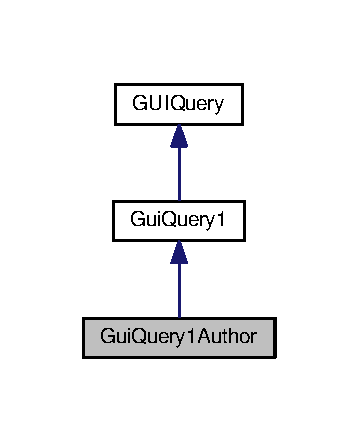
\includegraphics[width=172pt]{classGuiQuery1Author__inherit__graph}
\end{center}
\end{figure}


Collaboration diagram for Gui\+Query1\+Author\+:\nopagebreak
\begin{figure}[H]
\begin{center}
\leavevmode
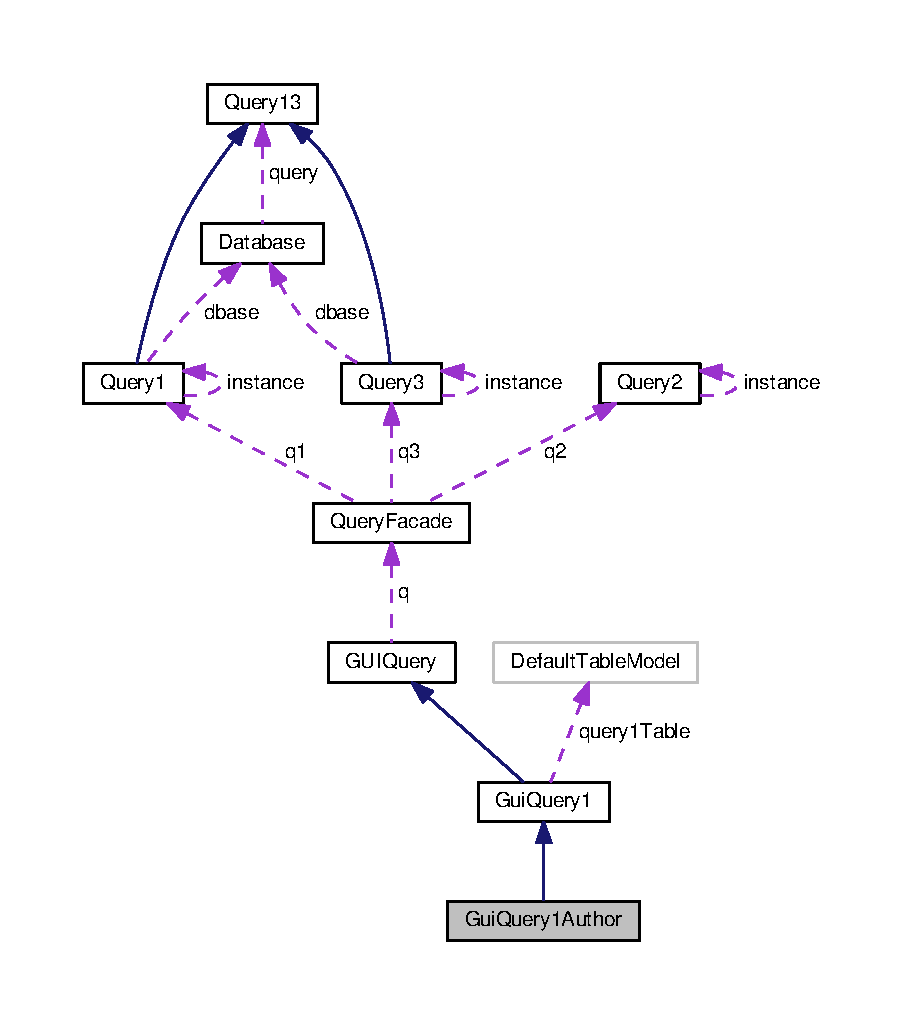
\includegraphics[width=350pt]{classGuiQuery1Author__coll__graph}
\end{center}
\end{figure}
\subsection*{Public Member Functions}
\begin{DoxyCompactItemize}
\item 
\hyperlink{classGuiQuery1Author_a7c4bd2b044d83f7a547ac78dcb29c914}{Gui\+Query1\+Author} (J\+Frame \hyperlink{classGUIQuery_aba988b5bec899d53480a472de7b87dfa}{main\+Frame}, J\+Combo\+Box$<$ String $>$ \hyperlink{classGUIQuery_a0db8bd960b4512cadf9aa40642934680}{queries}, J\+Panel \hyperlink{classGUIQuery_a70e233b1f14874166b7707edebe825d2}{side\+Panel}, J\+Panel \hyperlink{classGUIQuery_a8b4dbf257e0859c597591f072349b75c}{display\+Panel}, \hyperlink{classQueryFacade}{Query\+Facade} \hyperlink{classGUIQuery_a2a20445d749185552014142b78f3e071}{q}, J\+Combo\+Box$<$ String $>$ \hyperlink{classGuiQuery1_a021ae2f4fa2ec342496af6ac434995f4}{search\+By})
\item 
void \hyperlink{classGuiQuery1Author_ad86a9ba6fd82a330911b7267c25e7afe}{init\+State} ()
\item 
void \hyperlink{classGuiQuery1Author_a823956ef2ee980e1f907a55c2fc6f0b8}{init\+Author} ()
\item 
void \hyperlink{classGuiQuery1Author_a0bf8cce7ac52411d08c756b443be7b74}{set\+Query\+Author} ()
\end{DoxyCompactItemize}
\subsection*{Private Attributes}
\begin{DoxyCompactItemize}
\item 
final J\+Radio\+Button \hyperlink{classGuiQuery1Author_a5f63c8ecd9f332aadcbb7ec4c68dae30}{since\+Year} = new J\+Radio\+Button(\char`\"{}For Since year\char`\"{})
\item 
final J\+Radio\+Button \hyperlink{classGuiQuery1Author_a0ace1bd452a0f78fdda026280b168781}{custom\+Year} = new J\+Radio\+Button(\char`\"{}For custom year range\char`\"{})
\item 
Button\+Group \hyperlink{classGuiQuery1Author_a67b9d26988f566d493d8599a909d71e6}{year\+Buttons} = new Button\+Group()
\end{DoxyCompactItemize}
\subsection*{Additional Inherited Members}


\subsection{Detailed Description}
Creates the \hyperlink{classGUI}{G\+UI} \hyperlink{classQuery1}{Query1} search by author panel 

\subsection{Constructor \& Destructor Documentation}
\index{Gui\+Query1\+Author@{Gui\+Query1\+Author}!Gui\+Query1\+Author@{Gui\+Query1\+Author}}
\index{Gui\+Query1\+Author@{Gui\+Query1\+Author}!Gui\+Query1\+Author@{Gui\+Query1\+Author}}
\subsubsection[{\texorpdfstring{Gui\+Query1\+Author(\+J\+Frame main\+Frame, J\+Combo\+Box$<$ String $>$ queries, J\+Panel side\+Panel, J\+Panel display\+Panel, Query\+Facade q, J\+Combo\+Box$<$ String $>$ search\+By)}{GuiQuery1Author(JFrame mainFrame, JComboBox< String > queries, JPanel sidePanel, JPanel displayPanel, QueryFacade q, JComboBox< String > searchBy)}}]{\setlength{\rightskip}{0pt plus 5cm}Gui\+Query1\+Author.\+Gui\+Query1\+Author (
\begin{DoxyParamCaption}
\item[{J\+Frame}]{main\+Frame, }
\item[{J\+Combo\+Box$<$ String $>$}]{queries, }
\item[{J\+Panel}]{side\+Panel, }
\item[{J\+Panel}]{display\+Panel, }
\item[{{\bf Query\+Facade}}]{q, }
\item[{J\+Combo\+Box$<$ String $>$}]{search\+By}
\end{DoxyParamCaption}
)\hspace{0.3cm}{\ttfamily [inline]}}\hypertarget{classGuiQuery1Author_a7c4bd2b044d83f7a547ac78dcb29c914}{}\label{classGuiQuery1Author_a7c4bd2b044d83f7a547ac78dcb29c914}

\begin{DoxyCode}
25     \{
26         super(\hyperlink{classGUIQuery_aba988b5bec899d53480a472de7b87dfa}{mainFrame},\hyperlink{classGUIQuery_a0db8bd960b4512cadf9aa40642934680}{queries},\hyperlink{classGUIQuery_a70e233b1f14874166b7707edebe825d2}{sidePanel},\hyperlink{classGUIQuery_a8b4dbf257e0859c597591f072349b75c}{displayPanel},q,
      \hyperlink{classGuiQuery1_a021ae2f4fa2ec342496af6ac434995f4}{searchBy});
27         super.start();
28         \hyperlink{classGuiQuery1Author_a67b9d26988f566d493d8599a909d71e6}{yearButtons}.add(\hyperlink{classGuiQuery1Author_a5f63c8ecd9f332aadcbb7ec4c68dae30}{sinceYear});
29         \hyperlink{classGuiQuery1Author_a67b9d26988f566d493d8599a909d71e6}{yearButtons}.add(\hyperlink{classGuiQuery1Author_a0ace1bd452a0f78fdda026280b168781}{customYear});
30         \hyperlink{classGuiQuery1Author_a5f63c8ecd9f332aadcbb7ec4c68dae30}{sinceYear}.setBounds(60,200,150,15);
31         \hyperlink{classGuiQuery1Author_a0ace1bd452a0f78fdda026280b168781}{customYear}.setBounds(60,215,150,15);
32         \hyperlink{classGuiQuery1Author_a5f63c8ecd9f332aadcbb7ec4c68dae30}{sinceYear}.setFont(\textcolor{keyword}{new} Font(\textcolor{stringliteral}{"Calibri"}, Font.PLAIN, 10));
33         \hyperlink{classGuiQuery1Author_a0ace1bd452a0f78fdda026280b168781}{customYear}.setFont(\textcolor{keyword}{new} Font(\textcolor{stringliteral}{"Calibri"}, Font.PLAIN, 10));
34         \hyperlink{classGuiQuery1_a46ee2c343bc43a1c9a6278d9520b31f2}{flag}=0;
35         flag2=0;
36         \hyperlink{classGuiQuery1_a021ae2f4fa2ec342496af6ac434995f4}{searchBy}.setSelectedItem(\textcolor{stringliteral}{"Author Name"});
37         \textcolor{keywordflow}{try}\{
38             \hyperlink{classGuiQuery1_a021ae2f4fa2ec342496af6ac434995f4}{searchBy}.removeItem(\textcolor{stringliteral}{"Search By"});
39         \} \textcolor{keywordflow}{catch} (Exception e)\{\}
40         \hyperlink{classGUIQuery_a70e233b1f14874166b7707edebe825d2}{sidePanel}.removeAll();
41         \hyperlink{classGUIQuery_a8b4dbf257e0859c597591f072349b75c}{displayPanel}.removeAll();
42         \hyperlink{classGUIQuery_a70e233b1f14874166b7707edebe825d2}{sidePanel}.add(\hyperlink{classGuiQuery1_a021ae2f4fa2ec342496af6ac434995f4}{searchBy});
43         \hyperlink{classGUIQuery_a70e233b1f14874166b7707edebe825d2}{sidePanel}.add(\hyperlink{classGUIQuery_a0db8bd960b4512cadf9aa40642934680}{queries});
44         \hyperlink{classGUIQuery_a70e233b1f14874166b7707edebe825d2}{sidePanel}.add(\hyperlink{classGuiQuery1_a31e28191d4f156f0367a7dac29b65836}{title1});
45         \hyperlink{classGUIQuery_a70e233b1f14874166b7707edebe825d2}{sidePanel}.add(\hyperlink{classGuiQuery1_aeebb26c926dc7045d9bd99dd3568eb45}{title});
46         \hyperlink{classGUIQuery_a70e233b1f14874166b7707edebe825d2}{sidePanel}.add(\hyperlink{classGuiQuery1_ad120c79c1fe5e4b3ce09960942924c0d}{title2});
47         \hyperlink{classGUIQuery_a70e233b1f14874166b7707edebe825d2}{sidePanel}.add(\hyperlink{classGuiQuery1_a8659841dac2a5dcf9b367a7b19a19a52}{year1});
48         \hyperlink{classGUIQuery_a70e233b1f14874166b7707edebe825d2}{sidePanel}.add(\hyperlink{classGuiQuery1_a8e28412d9118fc61abde587c3bf7574f}{title3});
49         \hyperlink{classGUIQuery_a70e233b1f14874166b7707edebe825d2}{sidePanel}.add(\hyperlink{classGuiQuery1_a012c8e122c0a83d0af4ca51d03932c37}{year2});
50         \hyperlink{classGUIQuery_a70e233b1f14874166b7707edebe825d2}{sidePanel}.add(\hyperlink{classGuiQuery1_a40b4913205157f6e39c46956654a11f2}{dash});
51         \hyperlink{classGUIQuery_a70e233b1f14874166b7707edebe825d2}{sidePanel}.add(\hyperlink{classGuiQuery1_ac74d62ae05c068aaa998c52121501978}{year3});
52         \hyperlink{classGUIQuery_a70e233b1f14874166b7707edebe825d2}{sidePanel}.add(\hyperlink{classGUIQuery_a6580b15e365bc754c1a5ccdd2d58a4bb}{submit});
53         \hyperlink{classGUIQuery_a70e233b1f14874166b7707edebe825d2}{sidePanel}.add(reset);
54         \hyperlink{classGUIQuery_a70e233b1f14874166b7707edebe825d2}{sidePanel}.add(\hyperlink{classGuiQuery1_a382ff58e8c0283a69f6d88249b1fe496}{warning});
55         \hyperlink{classGUIQuery_a70e233b1f14874166b7707edebe825d2}{sidePanel}.add(\hyperlink{classGuiQuery1Author_a5f63c8ecd9f332aadcbb7ec4c68dae30}{sinceYear});
56         \hyperlink{classGUIQuery_a70e233b1f14874166b7707edebe825d2}{sidePanel}.add(\hyperlink{classGuiQuery1Author_a0ace1bd452a0f78fdda026280b168781}{customYear});   
57         \hyperlink{classGuiQuery1Author_a823956ef2ee980e1f907a55c2fc6f0b8}{initAuthor}();
58     \}
\end{DoxyCode}


\subsection{Member Function Documentation}
\index{Gui\+Query1\+Author@{Gui\+Query1\+Author}!init\+Author@{init\+Author}}
\index{init\+Author@{init\+Author}!Gui\+Query1\+Author@{Gui\+Query1\+Author}}
\subsubsection[{\texorpdfstring{init\+Author()}{initAuthor()}}]{\setlength{\rightskip}{0pt plus 5cm}void Gui\+Query1\+Author.\+init\+Author (
\begin{DoxyParamCaption}
{}
\end{DoxyParamCaption}
)\hspace{0.3cm}{\ttfamily [inline]}}\hypertarget{classGuiQuery1Author_a823956ef2ee980e1f907a55c2fc6f0b8}{}\label{classGuiQuery1Author_a823956ef2ee980e1f907a55c2fc6f0b8}

\begin{DoxyCode}
75     \{   
76         \hyperlink{classGUIQuery_a8b4dbf257e0859c597591f072349b75c}{displayPanel}.add(\hyperlink{classGuiQuery1_a515a1ac46f1362d811dd6e0c27d842fc}{totalResults});
77         \hyperlink{classGUIQuery_a8b4dbf257e0859c597591f072349b75c}{displayPanel}.add(\hyperlink{classGuiQuery1_aaa4f69c2faaffb0b451f1fa5bfebc4d3}{dispTable});
78         \hyperlink{classGUIQuery_a8b4dbf257e0859c597591f072349b75c}{displayPanel}.add(\hyperlink{classGuiQuery1_a0ef1bc892139ef28ea2e6c464f78e881}{next});
79         \hyperlink{classGUIQuery_aba988b5bec899d53480a472de7b87dfa}{mainFrame}.revalidate();
80         \hyperlink{classGUIQuery_aba988b5bec899d53480a472de7b87dfa}{mainFrame}.repaint();
81         tableWorking=0;
82         pages=0;
83         \hyperlink{classGuiQuery1Author_a5f63c8ecd9f332aadcbb7ec4c68dae30}{sinceYear}.addItemListener(\textcolor{keyword}{new} ItemListener() \{
84              \textcolor{keyword}{public} \textcolor{keywordtype}{void} itemStateChanged(ItemEvent e) \{         
85                         \hyperlink{classGuiQuery1_aa78daa5f76f85f27e3bbde79748bd34d}{changeMode}(1);    
86                 \}           
87           \});
88         
89         \hyperlink{classGuiQuery1Author_a0ace1bd452a0f78fdda026280b168781}{customYear}.addItemListener(\textcolor{keyword}{new} ItemListener() \{
90              \textcolor{keyword}{public} \textcolor{keywordtype}{void} itemStateChanged(ItemEvent e) \{    
91                 \hyperlink{classGuiQuery1_aa78daa5f76f85f27e3bbde79748bd34d}{changeMode}(2);
92              \}           
93           \});
94         reset.addActionListener(\textcolor{keyword}{new} ActionListener()\{
95                 \textcolor{keyword}{public} \textcolor{keywordtype}{void} actionPerformed(ActionEvent e)\{
96                     \hyperlink{classGuiQuery1Author_ad86a9ba6fd82a330911b7267c25e7afe}{initState}();\}
97             \});
98     \}
\end{DoxyCode}
\index{Gui\+Query1\+Author@{Gui\+Query1\+Author}!init\+State@{init\+State}}
\index{init\+State@{init\+State}!Gui\+Query1\+Author@{Gui\+Query1\+Author}}
\subsubsection[{\texorpdfstring{init\+State()}{initState()}}]{\setlength{\rightskip}{0pt plus 5cm}void Gui\+Query1\+Author.\+init\+State (
\begin{DoxyParamCaption}
{}
\end{DoxyParamCaption}
)\hspace{0.3cm}{\ttfamily [inline]}}\hypertarget{classGuiQuery1Author_ad86a9ba6fd82a330911b7267c25e7afe}{}\label{classGuiQuery1Author_ad86a9ba6fd82a330911b7267c25e7afe}

\begin{DoxyCode}
60     \{
61         \hyperlink{classGuiQuery1_a382ff58e8c0283a69f6d88249b1fe496}{warning}.setText(\textcolor{stringliteral}{" "});
62         \hyperlink{classGuiQuery1_a515a1ac46f1362d811dd6e0c27d842fc}{totalResults}.setText(\textcolor{stringliteral}{""});
63         tableWorking=0;
64         flag2=0;
65         \hyperlink{classGuiQuery1_a46ee2c343bc43a1c9a6278d9520b31f2}{flag}=0; 
66         \hyperlink{classGuiQuery1_ab9463b1a4a59d6c13bc04963b2b3f2c2}{query1Table}.setRowCount(0);
67         \hyperlink{classGuiQuery1_aeebb26c926dc7045d9bd99dd3568eb45}{title}.setText(\textcolor{stringliteral}{""}); 
68         \hyperlink{classGuiQuery1_a8659841dac2a5dcf9b367a7b19a19a52}{year1}.setText(\textcolor{stringliteral}{""}); 
69         \hyperlink{classGuiQuery1_a012c8e122c0a83d0af4ca51d03932c37}{year2}.setText(\textcolor{stringliteral}{""});         
70         \hyperlink{classGuiQuery1_ac74d62ae05c068aaa998c52121501978}{year3}.setText(\textcolor{stringliteral}{""});     
71         \hyperlink{classGuiQuery1Author_a67b9d26988f566d493d8599a909d71e6}{yearButtons}.clearSelection();
72         \hyperlink{classGuiQuery1_aa78daa5f76f85f27e3bbde79748bd34d}{changeMode}(0);    
73     \}
\end{DoxyCode}
\index{Gui\+Query1\+Author@{Gui\+Query1\+Author}!set\+Query\+Author@{set\+Query\+Author}}
\index{set\+Query\+Author@{set\+Query\+Author}!Gui\+Query1\+Author@{Gui\+Query1\+Author}}
\subsubsection[{\texorpdfstring{set\+Query\+Author()}{setQueryAuthor()}}]{\setlength{\rightskip}{0pt plus 5cm}void Gui\+Query1\+Author.\+set\+Query\+Author (
\begin{DoxyParamCaption}
{}
\end{DoxyParamCaption}
)\hspace{0.3cm}{\ttfamily [inline]}}\hypertarget{classGuiQuery1Author_a0bf8cce7ac52411d08c756b443be7b74}{}\label{classGuiQuery1Author_a0bf8cce7ac52411d08c756b443be7b74}

\begin{DoxyCode}
100                                  \{
101         \hyperlink{classGUIQuery_a6580b15e365bc754c1a5ccdd2d58a4bb}{submit}.addActionListener(\textcolor{keyword}{new} ActionListener()\{
102             \textcolor{keyword}{public} \textcolor{keywordtype}{void} actionPerformed(ActionEvent e)\{
103                 \hyperlink{classGuiQuery1_a382ff58e8c0283a69f6d88249b1fe496}{warning}.setText(\textcolor{stringliteral}{" "});
104                 \hyperlink{classGuiQuery1_a515a1ac46f1362d811dd6e0c27d842fc}{totalResults}.setText(\textcolor{stringliteral}{" "});
105                 \textcolor{keywordtype}{int} count=0;
106                 \hyperlink{classGuiQuery1_ab9463b1a4a59d6c13bc04963b2b3f2c2}{query1Table}.setRowCount(0);
107                 \textcolor{keywordtype}{int} y1=0,y2=0;
108                 \textcolor{keywordflow}{if}(flag2==1)\{
109                     \textcolor{keywordflow}{if}(\hyperlink{classGUIQuery_a2ffddedac70e763f8d4bfc6d24d9a0db}{isInteger}(\hyperlink{classGuiQuery1_a8659841dac2a5dcf9b367a7b19a19a52}{year1}.getText()))\{
110                         y1=Integer.parseInt(\hyperlink{classGuiQuery1_a8659841dac2a5dcf9b367a7b19a19a52}{year1}.getText());
111                     \} \textcolor{keywordflow}{else} \{
112                             \hyperlink{classGuiQuery1_a382ff58e8c0283a69f6d88249b1fe496}{warning}.setText(\textcolor{stringliteral}{"Year field should be numbers"});
113                         \}
114                     y2=9999;
115                 \} \textcolor{keywordflow}{else} \textcolor{keywordflow}{if} (flag2==2) \{
116                     \textcolor{keywordflow}{if}(\hyperlink{classGUIQuery_a2ffddedac70e763f8d4bfc6d24d9a0db}{isInteger}(\hyperlink{classGuiQuery1_a012c8e122c0a83d0af4ca51d03932c37}{year2}.getText())&&\hyperlink{classGUIQuery_a2ffddedac70e763f8d4bfc6d24d9a0db}{isInteger}(
      \hyperlink{classGuiQuery1_ac74d62ae05c068aaa998c52121501978}{year3}.getText()))  \{
117                         y1=Integer.parseInt(\hyperlink{classGuiQuery1_a012c8e122c0a83d0af4ca51d03932c37}{year2}.getText());
118                         y2=Integer.parseInt(\hyperlink{classGuiQuery1_ac74d62ae05c068aaa998c52121501978}{year3}.getText());
119                     \} \textcolor{keywordflow}{else} \{
120                         \hyperlink{classGuiQuery1_a382ff58e8c0283a69f6d88249b1fe496}{warning}.setText(\textcolor{stringliteral}{"Year field should be numbers"}); \}
121                 \} \textcolor{keywordflow}{else} \{
122                     y1=0;
123                     y2=9999;\}
124                 \textcolor{keywordflow}{if}(\hyperlink{classGuiQuery1_a382ff58e8c0283a69f6d88249b1fe496}{warning}.getText().equals(\textcolor{stringliteral}{" "}))\{
125                     \textcolor{keywordflow}{if}(\hyperlink{classGuiQuery1_aeebb26c926dc7045d9bd99dd3568eb45}{title}.getText().length()==0)\{
126                         \hyperlink{classGuiQuery1_a382ff58e8c0283a69f6d88249b1fe496}{warning}.setText(\textcolor{stringliteral}{"Author/Title field cannot be empty"});
127                     \}\textcolor{keywordflow}{else}\{
128                         \textcolor{keywordflow}{if}(\hyperlink{classGuiQuery1_a46ee2c343bc43a1c9a6278d9520b31f2}{flag}==0 || \hyperlink{classGuiQuery1_a46ee2c343bc43a1c9a6278d9520b31f2}{flag} ==1)\{
129                                 pages=0;
130                                 \hyperlink{classGUIQuery_a2a20445d749185552014142b78f3e071}{q}.\hyperlink{classQueryFacade_ac92989cd2e594e7c33191b16d7aced66}{queryOneFind}(1, \hyperlink{classGuiQuery1_aeebb26c926dc7045d9bd99dd3568eb45}{title}.getText(),y1,y2,
      \hyperlink{classGuiQuery1_a46ee2c343bc43a1c9a6278d9520b31f2}{flag});
131                                 \textcolor{keywordflow}{if}(\hyperlink{classGUIQuery_a2a20445d749185552014142b78f3e071}{q}.\hyperlink{classQueryFacade_a9c560f383a78c0757847bf898b647dfa}{queryOneGetCount}()==0)\{
132                                     \hyperlink{classGuiQuery1_a515a1ac46f1362d811dd6e0c27d842fc}{totalResults}.setText(\textcolor{stringliteral}{"No Result Found"});
133                                 \} \textcolor{keywordflow}{else}\{
134                                     \hyperlink{classGuiQuery1_a515a1ac46f1362d811dd6e0c27d842fc}{totalResults}.setText(\textcolor{stringliteral}{"Total results = "}+
      \hyperlink{classGUIQuery_a2a20445d749185552014142b78f3e071}{q}.\hyperlink{classQueryFacade_a9c560f383a78c0757847bf898b647dfa}{queryOneGetCount}());\}
135                                 tableWorking=1;
136                                 \hyperlink{classDataRecords}{DataRecords} d= \hyperlink{classGUIQuery_a2a20445d749185552014142b78f3e071}{q}.\hyperlink{classQueryFacade_adf9324b3f38765b2b6c1b4a64b301a11}{queryOneGetData}();
137                                 \textcolor{keywordflow}{while}(d!=null && count<20) \{
138                                     \hyperlink{classGuiQuery1_ab9463b1a4a59d6c13bc04963b2b3f2c2}{query1Table}.addRow(\textcolor{keyword}{new} Object[]\{count+1,d.
      \hyperlink{classDataRecords_a9b0dba84ec8d539395853caff7d4080f}{getAuthor}(),d.\hyperlink{classDataRecords_a2b6d27b078eb3a16734562f9ded6e1c6}{getTitle}(),d.\hyperlink{classDataRecords_a484260b5897ee754d22bdb1e0b1a4d69}{getPages}(),d.\hyperlink{classDataRecords_a9918de1a257be6b753ef46d66c43989c}{getYear}(),d.
      \hyperlink{classDataRecords_a6dfac293f0bd901eebf3a6ae17dc2513}{getVolume}(),d.\hyperlink{classDataRecords_add5c32b5a1511c42f70846fe08a4cfd7}{getJournalTitle}(),d.\hyperlink{classDataRecords_a40351f370945cfa624e1e3e1d6addc3e}{getURL}()\});
139                                     count++;
140                                     \textcolor{keywordflow}{if}(count<20)
141                                     \{d=\hyperlink{classGUIQuery_a2a20445d749185552014142b78f3e071}{q}.\hyperlink{classQueryFacade_adf9324b3f38765b2b6c1b4a64b301a11}{queryOneGetData}();\}    
142                                 \}
143                                 pages=1;
144                             \}   
145                         \}
146                     \}\textcolor{keywordflow}{else} \{ \}   
147                 \}
148         \});
149     \}   
\end{DoxyCode}


\subsection{Member Data Documentation}
\index{Gui\+Query1\+Author@{Gui\+Query1\+Author}!custom\+Year@{custom\+Year}}
\index{custom\+Year@{custom\+Year}!Gui\+Query1\+Author@{Gui\+Query1\+Author}}
\subsubsection[{\texorpdfstring{custom\+Year}{customYear}}]{\setlength{\rightskip}{0pt plus 5cm}final J\+Radio\+Button Gui\+Query1\+Author.\+custom\+Year = new J\+Radio\+Button(\char`\"{}For custom year range\char`\"{})\hspace{0.3cm}{\ttfamily [private]}}\hypertarget{classGuiQuery1Author_a0ace1bd452a0f78fdda026280b168781}{}\label{classGuiQuery1Author_a0ace1bd452a0f78fdda026280b168781}
\index{Gui\+Query1\+Author@{Gui\+Query1\+Author}!since\+Year@{since\+Year}}
\index{since\+Year@{since\+Year}!Gui\+Query1\+Author@{Gui\+Query1\+Author}}
\subsubsection[{\texorpdfstring{since\+Year}{sinceYear}}]{\setlength{\rightskip}{0pt plus 5cm}final J\+Radio\+Button Gui\+Query1\+Author.\+since\+Year = new J\+Radio\+Button(\char`\"{}For Since year\char`\"{})\hspace{0.3cm}{\ttfamily [private]}}\hypertarget{classGuiQuery1Author_a5f63c8ecd9f332aadcbb7ec4c68dae30}{}\label{classGuiQuery1Author_a5f63c8ecd9f332aadcbb7ec4c68dae30}
\index{Gui\+Query1\+Author@{Gui\+Query1\+Author}!year\+Buttons@{year\+Buttons}}
\index{year\+Buttons@{year\+Buttons}!Gui\+Query1\+Author@{Gui\+Query1\+Author}}
\subsubsection[{\texorpdfstring{year\+Buttons}{yearButtons}}]{\setlength{\rightskip}{0pt plus 5cm}Button\+Group Gui\+Query1\+Author.\+year\+Buttons = new Button\+Group()\hspace{0.3cm}{\ttfamily [private]}}\hypertarget{classGuiQuery1Author_a67b9d26988f566d493d8599a909d71e6}{}\label{classGuiQuery1Author_a67b9d26988f566d493d8599a909d71e6}


The documentation for this class was generated from the following file\+:\begin{DoxyCompactItemize}
\item 
\hyperlink{GuiQuery1Author_8java}{Gui\+Query1\+Author.\+java}\end{DoxyCompactItemize}

\hypertarget{classGuiQuery1Control}{}\section{Gui\+Query1\+Control Class Reference}
\label{classGuiQuery1Control}\index{Gui\+Query1\+Control@{Gui\+Query1\+Control}}


Inheritance diagram for Gui\+Query1\+Control\+:\nopagebreak
\begin{figure}[H]
\begin{center}
\leavevmode
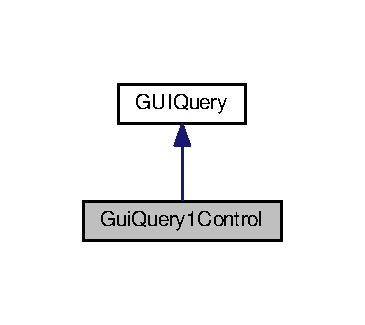
\includegraphics[width=175pt]{classGuiQuery1Control__inherit__graph}
\end{center}
\end{figure}


Collaboration diagram for Gui\+Query1\+Control\+:\nopagebreak
\begin{figure}[H]
\begin{center}
\leavevmode
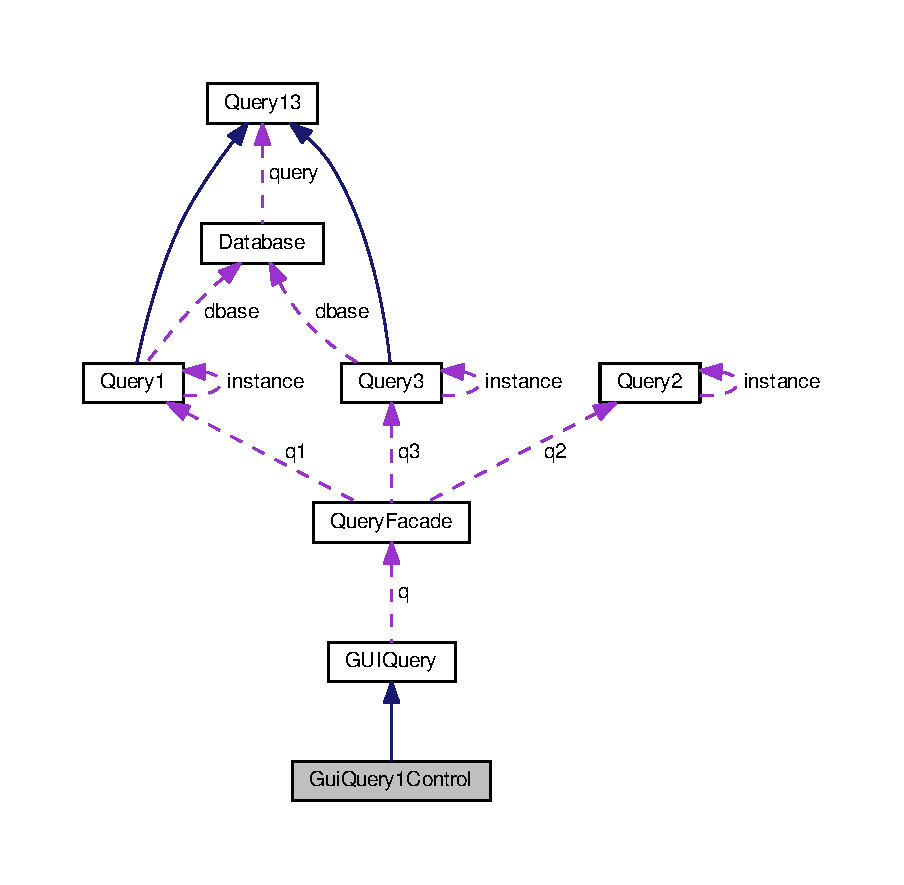
\includegraphics[width=350pt]{classGuiQuery1Control__coll__graph}
\end{center}
\end{figure}
\subsection*{Public Member Functions}
\begin{DoxyCompactItemize}
\item 
\hyperlink{classGuiQuery1Control_ac6989198b8ec672bd3d5329c98f0fe0a}{Gui\+Query1\+Control} (J\+Frame \hyperlink{classGUIQuery_aba988b5bec899d53480a472de7b87dfa}{main\+Frame}, J\+Combo\+Box$<$ String $>$ \hyperlink{classGUIQuery_a0db8bd960b4512cadf9aa40642934680}{queries}, J\+Panel \hyperlink{classGUIQuery_a70e233b1f14874166b7707edebe825d2}{side\+Panel}, J\+Panel \hyperlink{classGUIQuery_a8b4dbf257e0859c597591f072349b75c}{display\+Panel}, \hyperlink{classQueryFacade}{Query\+Facade} q1)
\item 
void \hyperlink{classGuiQuery1Control_a9d83b448fb4105b5a2c4c4902a7a1d49}{init\+Query} ()
\item 
void \hyperlink{classGuiQuery1Control_a7cf6dca14e3622abc057feff8c28260e}{set\+Query} ()
\end{DoxyCompactItemize}
\subsection*{Private Attributes}
\begin{DoxyCompactItemize}
\item 
J\+Combo\+Box$<$ String $>$ \hyperlink{classGuiQuery1Control_aff1971237254429cafcc0c76a1937793}{search\+By} = new J\+Combo\+Box$<$String$>$()
\end{DoxyCompactItemize}
\subsection*{Additional Inherited Members}


\subsection{Detailed Description}
Controls how \hyperlink{classQuery1}{Query1} functions 

\subsection{Constructor \& Destructor Documentation}
\index{Gui\+Query1\+Control@{Gui\+Query1\+Control}!Gui\+Query1\+Control@{Gui\+Query1\+Control}}
\index{Gui\+Query1\+Control@{Gui\+Query1\+Control}!Gui\+Query1\+Control@{Gui\+Query1\+Control}}
\subsubsection[{\texorpdfstring{Gui\+Query1\+Control(\+J\+Frame main\+Frame, J\+Combo\+Box$<$ String $>$ queries, J\+Panel side\+Panel, J\+Panel display\+Panel, Query\+Facade q1)}{GuiQuery1Control(JFrame mainFrame, JComboBox< String > queries, JPanel sidePanel, JPanel displayPanel, QueryFacade q1)}}]{\setlength{\rightskip}{0pt plus 5cm}Gui\+Query1\+Control.\+Gui\+Query1\+Control (
\begin{DoxyParamCaption}
\item[{J\+Frame}]{main\+Frame, }
\item[{J\+Combo\+Box$<$ String $>$}]{queries, }
\item[{J\+Panel}]{side\+Panel, }
\item[{J\+Panel}]{display\+Panel, }
\item[{{\bf Query\+Facade}}]{q1}
\end{DoxyParamCaption}
)\hspace{0.3cm}{\ttfamily [inline]}}\hypertarget{classGuiQuery1Control_ac6989198b8ec672bd3d5329c98f0fe0a}{}\label{classGuiQuery1Control_ac6989198b8ec672bd3d5329c98f0fe0a}

\begin{DoxyCode}
23     \{
24         this.\hyperlink{classGUIQuery_aba988b5bec899d53480a472de7b87dfa}{mainFrame}=\hyperlink{classGUIQuery_aba988b5bec899d53480a472de7b87dfa}{mainFrame};
25         this.\hyperlink{classGUIQuery_a0db8bd960b4512cadf9aa40642934680}{queries}=\hyperlink{classGUIQuery_a0db8bd960b4512cadf9aa40642934680}{queries};
26         this.\hyperlink{classGUIQuery_a70e233b1f14874166b7707edebe825d2}{sidePanel}=\hyperlink{classGUIQuery_a70e233b1f14874166b7707edebe825d2}{sidePanel};
27         this.\hyperlink{classGUIQuery_a8b4dbf257e0859c597591f072349b75c}{displayPanel}=\hyperlink{classGUIQuery_a8b4dbf257e0859c597591f072349b75c}{displayPanel};
28         this.\hyperlink{classGUIQuery_a2a20445d749185552014142b78f3e071}{q}=q1;
29         \hyperlink{classGuiQuery1Control_aff1971237254429cafcc0c76a1937793}{searchBy}.addItem(\textcolor{stringliteral}{"Search By"});
30         \hyperlink{classGuiQuery1Control_aff1971237254429cafcc0c76a1937793}{searchBy}.addItem(\textcolor{stringliteral}{"Author Name"});
31         \hyperlink{classGuiQuery1Control_aff1971237254429cafcc0c76a1937793}{searchBy}.addItem(\textcolor{stringliteral}{"Title Tag"});
32         \hyperlink{classGuiQuery1Control_aff1971237254429cafcc0c76a1937793}{searchBy}.setSelectedItem(\textcolor{stringliteral}{"Search By"});
33         \hyperlink{classGuiQuery1Control_aff1971237254429cafcc0c76a1937793}{searchBy}.setBounds(50,50,100,20);
34         \hyperlink{classGuiQuery1Control_aff1971237254429cafcc0c76a1937793}{searchBy}.setFont(\textcolor{keyword}{new} Font(\textcolor{stringliteral}{"Calibri"}, Font.PLAIN, 10));
35     \}
\end{DoxyCode}


\subsection{Member Function Documentation}
\index{Gui\+Query1\+Control@{Gui\+Query1\+Control}!init\+Query@{init\+Query}}
\index{init\+Query@{init\+Query}!Gui\+Query1\+Control@{Gui\+Query1\+Control}}
\subsubsection[{\texorpdfstring{init\+Query()}{initQuery()}}]{\setlength{\rightskip}{0pt plus 5cm}void Gui\+Query1\+Control.\+init\+Query (
\begin{DoxyParamCaption}
{}
\end{DoxyParamCaption}
)\hspace{0.3cm}{\ttfamily [inline]}}\hypertarget{classGuiQuery1Control_a9d83b448fb4105b5a2c4c4902a7a1d49}{}\label{classGuiQuery1Control_a9d83b448fb4105b5a2c4c4902a7a1d49}

\begin{DoxyCode}
38     \{
39         
40     \}
\end{DoxyCode}
\index{Gui\+Query1\+Control@{Gui\+Query1\+Control}!set\+Query@{set\+Query}}
\index{set\+Query@{set\+Query}!Gui\+Query1\+Control@{Gui\+Query1\+Control}}
\subsubsection[{\texorpdfstring{set\+Query()}{setQuery()}}]{\setlength{\rightskip}{0pt plus 5cm}void Gui\+Query1\+Control.\+set\+Query (
\begin{DoxyParamCaption}
{}
\end{DoxyParamCaption}
)\hspace{0.3cm}{\ttfamily [inline]}}\hypertarget{classGuiQuery1Control_a7cf6dca14e3622abc057feff8c28260e}{}\label{classGuiQuery1Control_a7cf6dca14e3622abc057feff8c28260e}

\begin{DoxyCode}
43     \{
44         \hyperlink{classGUIQuery_a0db8bd960b4512cadf9aa40642934680}{queries}.removeItem(\textcolor{stringliteral}{"Queries"});
45         \hyperlink{classGUIQuery_a70e233b1f14874166b7707edebe825d2}{sidePanel}.removeAll();
46         \hyperlink{classGUIQuery_a8b4dbf257e0859c597591f072349b75c}{displayPanel}.removeAll();
47         \hyperlink{classGUIQuery_a0db8bd960b4512cadf9aa40642934680}{queries}.setBounds(50,20,100,20);
48         \hyperlink{classGUIQuery_a0db8bd960b4512cadf9aa40642934680}{queries}.setSelectedItem(\textcolor{stringliteral}{"Query 1"});
49         \textcolor{comment}{//----  }
50         \hyperlink{classGUIQuery_a70e233b1f14874166b7707edebe825d2}{sidePanel}.add(\hyperlink{classGuiQuery1Control_aff1971237254429cafcc0c76a1937793}{searchBy});
51         \hyperlink{classGUIQuery_a70e233b1f14874166b7707edebe825d2}{sidePanel}.add(\hyperlink{classGUIQuery_a0db8bd960b4512cadf9aa40642934680}{queries});
52         \hyperlink{classGUIQuery_aba988b5bec899d53480a472de7b87dfa}{mainFrame}.revalidate();
53         \hyperlink{classGUIQuery_aba988b5bec899d53480a472de7b87dfa}{mainFrame}.repaint();
54 
55         \hyperlink{classGuiQuery1Control_aff1971237254429cafcc0c76a1937793}{searchBy}.addActionListener(\textcolor{keyword}{new} ActionListener() \{
56             @Override
57             \textcolor{keyword}{public} \textcolor{keywordtype}{void} actionPerformed(ActionEvent event) \{
58                     JComboBox<? extends Object> t= (JComboBox<? extends Object>) event.getSource();
59                 String selectedQuery = (String) t.getSelectedItem();
60                 \textcolor{keywordflow}{if} (selectedQuery.equals(\textcolor{stringliteral}{"Author Name"})) \{
61                    \hyperlink{classGuiQuery1Author}{GuiQuery1Author} ga= \textcolor{keyword}{new} \hyperlink{classGuiQuery1Author}{GuiQuery1Author}(
      \hyperlink{classGUIQuery_aba988b5bec899d53480a472de7b87dfa}{mainFrame},\hyperlink{classGUIQuery_a0db8bd960b4512cadf9aa40642934680}{queries},\hyperlink{classGUIQuery_a70e233b1f14874166b7707edebe825d2}{sidePanel},\hyperlink{classGUIQuery_a8b4dbf257e0859c597591f072349b75c}{displayPanel},\hyperlink{classGUIQuery_a2a20445d749185552014142b78f3e071}{q},
      \hyperlink{classGuiQuery1Control_aff1971237254429cafcc0c76a1937793}{searchBy});
62                    ga.\hyperlink{classGuiQuery1Author_a0bf8cce7ac52411d08c756b443be7b74}{setQueryAuthor}();
63                 \}     \textcolor{keywordflow}{else} \textcolor{keywordflow}{if} (selectedQuery.equals(\textcolor{stringliteral}{"Title Tag"})) \{
64                     \hyperlink{classGuiQuery1Title}{GuiQuery1Title} gt= \textcolor{keyword}{new} \hyperlink{classGuiQuery1Title}{GuiQuery1Title}(
      \hyperlink{classGUIQuery_aba988b5bec899d53480a472de7b87dfa}{mainFrame},\hyperlink{classGUIQuery_a0db8bd960b4512cadf9aa40642934680}{queries},\hyperlink{classGUIQuery_a70e233b1f14874166b7707edebe825d2}{sidePanel},\hyperlink{classGUIQuery_a8b4dbf257e0859c597591f072349b75c}{displayPanel},\hyperlink{classGUIQuery_a2a20445d749185552014142b78f3e071}{q},
      \hyperlink{classGuiQuery1Control_aff1971237254429cafcc0c76a1937793}{searchBy});
65                    gt.\hyperlink{classGuiQuery1Title_ab549b18802bf2e90895154fbb4d9d51b}{setQueryTitle}();
66                 \}
67             \}
68         \});
69     \}   
\end{DoxyCode}


\subsection{Member Data Documentation}
\index{Gui\+Query1\+Control@{Gui\+Query1\+Control}!search\+By@{search\+By}}
\index{search\+By@{search\+By}!Gui\+Query1\+Control@{Gui\+Query1\+Control}}
\subsubsection[{\texorpdfstring{search\+By}{searchBy}}]{\setlength{\rightskip}{0pt plus 5cm}J\+Combo\+Box$<$String$>$ Gui\+Query1\+Control.\+search\+By = new J\+Combo\+Box$<$String$>$()\hspace{0.3cm}{\ttfamily [private]}}\hypertarget{classGuiQuery1Control_aff1971237254429cafcc0c76a1937793}{}\label{classGuiQuery1Control_aff1971237254429cafcc0c76a1937793}


The documentation for this class was generated from the following file\+:\begin{DoxyCompactItemize}
\item 
\hyperlink{GuiQuery1Control_8java}{Gui\+Query1\+Control.\+java}\end{DoxyCompactItemize}

\hypertarget{classGuiQuery1Title}{}\section{Gui\+Query1\+Title Class Reference}
\label{classGuiQuery1Title}\index{Gui\+Query1\+Title@{Gui\+Query1\+Title}}


Inheritance diagram for Gui\+Query1\+Title\+:\nopagebreak
\begin{figure}[H]
\begin{center}
\leavevmode
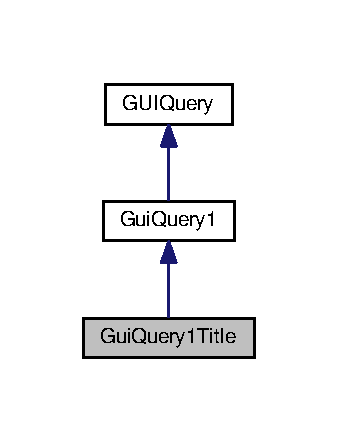
\includegraphics[width=162pt]{classGuiQuery1Title__inherit__graph}
\end{center}
\end{figure}


Collaboration diagram for Gui\+Query1\+Title\+:\nopagebreak
\begin{figure}[H]
\begin{center}
\leavevmode
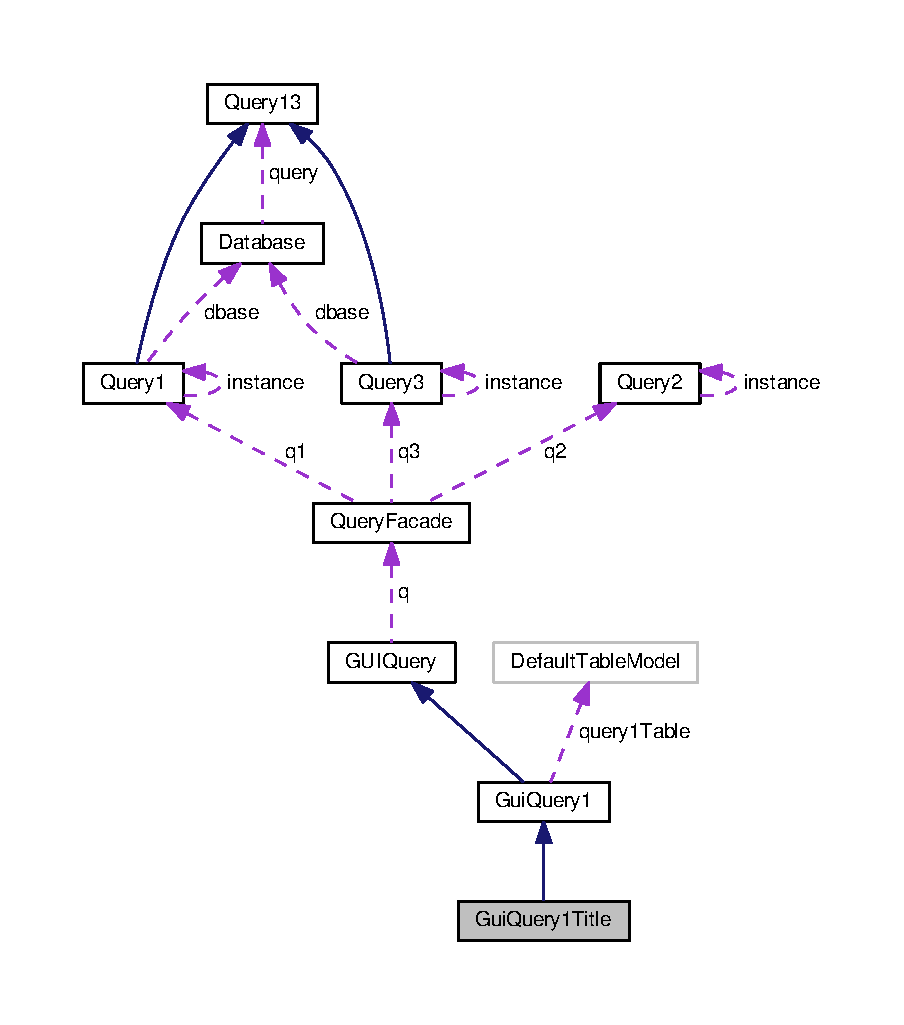
\includegraphics[width=350pt]{classGuiQuery1Title__coll__graph}
\end{center}
\end{figure}
\subsection*{Public Member Functions}
\begin{DoxyCompactItemize}
\item 
\hyperlink{classGuiQuery1Title_a1280b921b2d0ad92b60e8053e0e3c704}{Gui\+Query1\+Title} (J\+Frame \hyperlink{classGUIQuery_aba988b5bec899d53480a472de7b87dfa}{main\+Frame}, J\+Combo\+Box$<$ String $>$ \hyperlink{classGUIQuery_a0db8bd960b4512cadf9aa40642934680}{queries}, J\+Panel \hyperlink{classGUIQuery_a70e233b1f14874166b7707edebe825d2}{side\+Panel}, J\+Panel \hyperlink{classGUIQuery_a8b4dbf257e0859c597591f072349b75c}{display\+Panel}, \hyperlink{classQueryFacade}{Query\+Facade} \hyperlink{classGUIQuery_a2a20445d749185552014142b78f3e071}{q}, J\+Combo\+Box$<$ String $>$ \hyperlink{classGuiQuery1_a021ae2f4fa2ec342496af6ac434995f4}{search\+By})
\item 
void \hyperlink{classGuiQuery1Title_a5ef02fd3f5472ff67fc24efce9d47e50}{init\+Title} ()
\item 
void \hyperlink{classGuiQuery1Title_ab549b18802bf2e90895154fbb4d9d51b}{set\+Query\+Title} ()
\end{DoxyCompactItemize}
\subsection*{Private Attributes}
\begin{DoxyCompactItemize}
\item 
final J\+Radio\+Button \hyperlink{classGuiQuery1Title_aff3f4abd05828888c376d91e9c72ae3f}{sort\+Rel} = new J\+Radio\+Button(\char`\"{}Sort by Relevance\char`\"{})
\item 
final J\+Radio\+Button \hyperlink{classGuiQuery1Title_a282ba6983218ab020c0fe9b65a0c5619}{sort\+Year} = new J\+Radio\+Button(\char`\"{}Sort by Date\char`\"{},true)
\item 
Button\+Group \hyperlink{classGuiQuery1Title_a92ce684b789aae7c807f5041ac8f7b54}{sort\+Buttons} = new Button\+Group()
\item 
final J\+Radio\+Button \hyperlink{classGuiQuery1Title_a57f5240e22a35a95739062b91bdd4cba}{since\+Year} = new J\+Radio\+Button(\char`\"{}For Since year\char`\"{})
\item 
final J\+Radio\+Button \hyperlink{classGuiQuery1Title_aa7c8f24ee5498bd7808133f52a585449}{custom\+Year} = new J\+Radio\+Button(\char`\"{}For custom year range\char`\"{})
\item 
Button\+Group \hyperlink{classGuiQuery1Title_ac28a3c0196f225f9048778b102a57663}{year\+Buttons} = new Button\+Group()
\end{DoxyCompactItemize}
\subsection*{Additional Inherited Members}


\subsection{Detailed Description}
Creates the \hyperlink{classGUI}{G\+UI} \hyperlink{classQuery1}{Query1} search by title panel 

\subsection{Constructor \& Destructor Documentation}
\index{Gui\+Query1\+Title@{Gui\+Query1\+Title}!Gui\+Query1\+Title@{Gui\+Query1\+Title}}
\index{Gui\+Query1\+Title@{Gui\+Query1\+Title}!Gui\+Query1\+Title@{Gui\+Query1\+Title}}
\subsubsection[{\texorpdfstring{Gui\+Query1\+Title(\+J\+Frame main\+Frame, J\+Combo\+Box$<$ String $>$ queries, J\+Panel side\+Panel, J\+Panel display\+Panel, Query\+Facade q, J\+Combo\+Box$<$ String $>$ search\+By)}{GuiQuery1Title(JFrame mainFrame, JComboBox< String > queries, JPanel sidePanel, JPanel displayPanel, QueryFacade q, JComboBox< String > searchBy)}}]{\setlength{\rightskip}{0pt plus 5cm}Gui\+Query1\+Title.\+Gui\+Query1\+Title (
\begin{DoxyParamCaption}
\item[{J\+Frame}]{main\+Frame, }
\item[{J\+Combo\+Box$<$ String $>$}]{queries, }
\item[{J\+Panel}]{side\+Panel, }
\item[{J\+Panel}]{display\+Panel, }
\item[{{\bf Query\+Facade}}]{q, }
\item[{J\+Combo\+Box$<$ String $>$}]{search\+By}
\end{DoxyParamCaption}
)\hspace{0.3cm}{\ttfamily [inline]}}\hypertarget{classGuiQuery1Title_a1280b921b2d0ad92b60e8053e0e3c704}{}\label{classGuiQuery1Title_a1280b921b2d0ad92b60e8053e0e3c704}

\begin{DoxyCode}
28     \{
29         super(\hyperlink{classGUIQuery_aba988b5bec899d53480a472de7b87dfa}{mainFrame},\hyperlink{classGUIQuery_a0db8bd960b4512cadf9aa40642934680}{queries},\hyperlink{classGUIQuery_a70e233b1f14874166b7707edebe825d2}{sidePanel},\hyperlink{classGUIQuery_a8b4dbf257e0859c597591f072349b75c}{displayPanel},q,
      \hyperlink{classGuiQuery1_a021ae2f4fa2ec342496af6ac434995f4}{searchBy});
30         super.start();
31         \hyperlink{classGuiQuery1Title_a92ce684b789aae7c807f5041ac8f7b54}{sortButtons}.add(\hyperlink{classGuiQuery1Title_aff3f4abd05828888c376d91e9c72ae3f}{sortRel});
32         \hyperlink{classGuiQuery1Title_a92ce684b789aae7c807f5041ac8f7b54}{sortButtons}.add(\hyperlink{classGuiQuery1Title_a282ba6983218ab020c0fe9b65a0c5619}{sortYear});
33         \hyperlink{classGuiQuery1Title_a282ba6983218ab020c0fe9b65a0c5619}{sortYear}.setBounds(60,200,150,15);
34         \hyperlink{classGuiQuery1Title_aff3f4abd05828888c376d91e9c72ae3f}{sortRel}.setBounds(60,215,150,15);
35         \hyperlink{classGuiQuery1Title_a282ba6983218ab020c0fe9b65a0c5619}{sortYear}.setFont(\textcolor{keyword}{new} Font(\textcolor{stringliteral}{"Calibri"}, Font.PLAIN, 10));
36         \hyperlink{classGuiQuery1Title_aff3f4abd05828888c376d91e9c72ae3f}{sortRel}.setFont(\textcolor{keyword}{new} Font(\textcolor{stringliteral}{"Calibri"}, Font.PLAIN, 10));
37         \hyperlink{classGuiQuery1Title_ac28a3c0196f225f9048778b102a57663}{yearButtons}.add(\hyperlink{classGuiQuery1Title_a57f5240e22a35a95739062b91bdd4cba}{sinceYear});
38         \hyperlink{classGuiQuery1Title_ac28a3c0196f225f9048778b102a57663}{yearButtons}.add(\hyperlink{classGuiQuery1Title_aa7c8f24ee5498bd7808133f52a585449}{customYear});
39         \hyperlink{classGuiQuery1Title_a57f5240e22a35a95739062b91bdd4cba}{sinceYear}.setBounds(60,245,150,15);
40         \hyperlink{classGuiQuery1Title_aa7c8f24ee5498bd7808133f52a585449}{customYear}.setBounds(60,260,150,15);
41         \hyperlink{classGuiQuery1Title_a57f5240e22a35a95739062b91bdd4cba}{sinceYear}.setFont(\textcolor{keyword}{new} Font(\textcolor{stringliteral}{"Calibri"}, Font.PLAIN, 10));
42         \hyperlink{classGuiQuery1Title_aa7c8f24ee5498bd7808133f52a585449}{customYear}.setFont(\textcolor{keyword}{new} Font(\textcolor{stringliteral}{"Calibri"}, Font.PLAIN, 10));
43         \hyperlink{classGuiQuery1_a46ee2c343bc43a1c9a6278d9520b31f2}{flag}=0;
44         flag2=0;
45         \hyperlink{classGUIQuery_a70e233b1f14874166b7707edebe825d2}{sidePanel}.removeAll();
46         \hyperlink{classGUIQuery_a8b4dbf257e0859c597591f072349b75c}{displayPanel}.removeAll();
47         \hyperlink{classGuiQuery1_a021ae2f4fa2ec342496af6ac434995f4}{searchBy}.setSelectedItem(\textcolor{stringliteral}{"Title Tag"});
48         \textcolor{keywordflow}{try}\{
49             \hyperlink{classGuiQuery1_a021ae2f4fa2ec342496af6ac434995f4}{searchBy}.removeItem(\textcolor{stringliteral}{"Search By"});
50         \} \textcolor{keywordflow}{catch} (Exception e)\{\}
51         \hyperlink{classGUIQuery_a70e233b1f14874166b7707edebe825d2}{sidePanel}.add(\hyperlink{classGuiQuery1_a021ae2f4fa2ec342496af6ac434995f4}{searchBy});
52         \hyperlink{classGUIQuery_a70e233b1f14874166b7707edebe825d2}{sidePanel}.add(\hyperlink{classGUIQuery_a0db8bd960b4512cadf9aa40642934680}{queries});
53         \hyperlink{classGUIQuery_a70e233b1f14874166b7707edebe825d2}{sidePanel}.add(\hyperlink{classGuiQuery1_a31e28191d4f156f0367a7dac29b65836}{title1});
54         \hyperlink{classGUIQuery_a70e233b1f14874166b7707edebe825d2}{sidePanel}.add(\hyperlink{classGuiQuery1_aeebb26c926dc7045d9bd99dd3568eb45}{title});
55         \hyperlink{classGUIQuery_a70e233b1f14874166b7707edebe825d2}{sidePanel}.add(\hyperlink{classGuiQuery1_ad120c79c1fe5e4b3ce09960942924c0d}{title2});
56         \hyperlink{classGUIQuery_a70e233b1f14874166b7707edebe825d2}{sidePanel}.add(\hyperlink{classGuiQuery1_a8659841dac2a5dcf9b367a7b19a19a52}{year1});
57         \hyperlink{classGUIQuery_a70e233b1f14874166b7707edebe825d2}{sidePanel}.add(\hyperlink{classGuiQuery1_a8e28412d9118fc61abde587c3bf7574f}{title3});
58         \hyperlink{classGUIQuery_a70e233b1f14874166b7707edebe825d2}{sidePanel}.add(\hyperlink{classGuiQuery1_a012c8e122c0a83d0af4ca51d03932c37}{year2});
59         \hyperlink{classGUIQuery_a70e233b1f14874166b7707edebe825d2}{sidePanel}.add(\hyperlink{classGuiQuery1_a40b4913205157f6e39c46956654a11f2}{dash});
60         \hyperlink{classGUIQuery_a70e233b1f14874166b7707edebe825d2}{sidePanel}.add(\hyperlink{classGuiQuery1_ac74d62ae05c068aaa998c52121501978}{year3});
61         \hyperlink{classGUIQuery_a70e233b1f14874166b7707edebe825d2}{sidePanel}.add(\hyperlink{classGuiQuery1Title_a282ba6983218ab020c0fe9b65a0c5619}{sortYear});
62         \hyperlink{classGUIQuery_a70e233b1f14874166b7707edebe825d2}{sidePanel}.add(\hyperlink{classGuiQuery1Title_aff3f4abd05828888c376d91e9c72ae3f}{sortRel});
63         \hyperlink{classGUIQuery_a70e233b1f14874166b7707edebe825d2}{sidePanel}.add(\hyperlink{classGUIQuery_a6580b15e365bc754c1a5ccdd2d58a4bb}{submit});
64         \hyperlink{classGUIQuery_a70e233b1f14874166b7707edebe825d2}{sidePanel}.add(reset);
65         \hyperlink{classGUIQuery_a70e233b1f14874166b7707edebe825d2}{sidePanel}.add(\hyperlink{classGuiQuery1_a382ff58e8c0283a69f6d88249b1fe496}{warning});
66         \hyperlink{classGUIQuery_a70e233b1f14874166b7707edebe825d2}{sidePanel}.add(\hyperlink{classGuiQuery1Title_a57f5240e22a35a95739062b91bdd4cba}{sinceYear});
67         \hyperlink{classGUIQuery_a70e233b1f14874166b7707edebe825d2}{sidePanel}.add(\hyperlink{classGuiQuery1Title_aa7c8f24ee5498bd7808133f52a585449}{customYear});
68         \hyperlink{classGuiQuery1Title_a5ef02fd3f5472ff67fc24efce9d47e50}{initTitle}();
69     \}
\end{DoxyCode}


\subsection{Member Function Documentation}
\index{Gui\+Query1\+Title@{Gui\+Query1\+Title}!init\+Title@{init\+Title}}
\index{init\+Title@{init\+Title}!Gui\+Query1\+Title@{Gui\+Query1\+Title}}
\subsubsection[{\texorpdfstring{init\+Title()}{initTitle()}}]{\setlength{\rightskip}{0pt plus 5cm}void Gui\+Query1\+Title.\+init\+Title (
\begin{DoxyParamCaption}
{}
\end{DoxyParamCaption}
)\hspace{0.3cm}{\ttfamily [inline]}}\hypertarget{classGuiQuery1Title_a5ef02fd3f5472ff67fc24efce9d47e50}{}\label{classGuiQuery1Title_a5ef02fd3f5472ff67fc24efce9d47e50}

\begin{DoxyCode}
71                             \{
72         \hyperlink{classGUIQuery_a8b4dbf257e0859c597591f072349b75c}{displayPanel}.add(\hyperlink{classGuiQuery1_a515a1ac46f1362d811dd6e0c27d842fc}{totalResults});
73         \hyperlink{classGUIQuery_a8b4dbf257e0859c597591f072349b75c}{displayPanel}.add(\hyperlink{classGuiQuery1_aaa4f69c2faaffb0b451f1fa5bfebc4d3}{dispTable});
74         \hyperlink{classGUIQuery_a8b4dbf257e0859c597591f072349b75c}{displayPanel}.add(\hyperlink{classGuiQuery1_a0ef1bc892139ef28ea2e6c464f78e881}{next});
75         \hyperlink{classGUIQuery_aba988b5bec899d53480a472de7b87dfa}{mainFrame}.revalidate();
76         \hyperlink{classGUIQuery_aba988b5bec899d53480a472de7b87dfa}{mainFrame}.repaint();
77         tableWorking=0;
78         pages=0;
79         \hyperlink{classGuiQuery1Title_aff3f4abd05828888c376d91e9c72ae3f}{sortRel}.addItemListener(\textcolor{keyword}{new} ItemListener() \{
80              \textcolor{keyword}{public} \textcolor{keywordtype}{void} itemStateChanged(ItemEvent e) \{         
81                         \hyperlink{classGuiQuery1_abe08121cbcebdc066aaec8400bc73cc7}{change}(1);    
82                 \}           
83           \});
84         
85         \hyperlink{classGuiQuery1Title_a282ba6983218ab020c0fe9b65a0c5619}{sortYear}.addItemListener(\textcolor{keyword}{new} ItemListener() \{
86              \textcolor{keyword}{public} \textcolor{keywordtype}{void} itemStateChanged(ItemEvent e) \{         
87                 \hyperlink{classGuiQuery1_abe08121cbcebdc066aaec8400bc73cc7}{change}(0);
88              \}           
89           \});
90         \hyperlink{classGuiQuery1Title_a57f5240e22a35a95739062b91bdd4cba}{sinceYear}.addItemListener(\textcolor{keyword}{new} ItemListener() \{
91              \textcolor{keyword}{public} \textcolor{keywordtype}{void} itemStateChanged(ItemEvent e) \{         
92                         \hyperlink{classGuiQuery1_aa78daa5f76f85f27e3bbde79748bd34d}{changeMode}(1);    
93                 \}           
94           \});
95         
96         \hyperlink{classGuiQuery1Title_aa7c8f24ee5498bd7808133f52a585449}{customYear}.addItemListener(\textcolor{keyword}{new} ItemListener() \{
97              \textcolor{keyword}{public} \textcolor{keywordtype}{void} itemStateChanged(ItemEvent e) \{         
98                 \hyperlink{classGuiQuery1_aa78daa5f76f85f27e3bbde79748bd34d}{changeMode}(2);
99              \}           
100           \});
101         reset.addActionListener(\textcolor{keyword}{new} ActionListener()\{
102                 \textcolor{keyword}{public} \textcolor{keywordtype}{void} actionPerformed(ActionEvent e)\{
103                     \hyperlink{classGuiQuery1_a382ff58e8c0283a69f6d88249b1fe496}{warning}.setText(\textcolor{stringliteral}{" "});
104                     \hyperlink{classGuiQuery1_a515a1ac46f1362d811dd6e0c27d842fc}{totalResults}.setText(\textcolor{stringliteral}{""});
105                     tableWorking=0;
106                     \hyperlink{classGuiQuery1_ab9463b1a4a59d6c13bc04963b2b3f2c2}{query1Table}.setRowCount(0);
107                     \hyperlink{classGuiQuery1_aeebb26c926dc7045d9bd99dd3568eb45}{title}.setText(\textcolor{stringliteral}{""}); 
108                     \hyperlink{classGuiQuery1_a8659841dac2a5dcf9b367a7b19a19a52}{year1}.setText(\textcolor{stringliteral}{""}); 
109                     \hyperlink{classGuiQuery1_a012c8e122c0a83d0af4ca51d03932c37}{year2}.setText(\textcolor{stringliteral}{""});         
110                     \hyperlink{classGuiQuery1_ac74d62ae05c068aaa998c52121501978}{year3}.setText(\textcolor{stringliteral}{""});     
111                     \hyperlink{classGuiQuery1Title_a92ce684b789aae7c807f5041ac8f7b54}{sortButtons}.clearSelection();
112                     \hyperlink{classGuiQuery1Title_ac28a3c0196f225f9048778b102a57663}{yearButtons}.clearSelection();
113                     \hyperlink{classGuiQuery1Title_a282ba6983218ab020c0fe9b65a0c5619}{sortYear}.setSelected(\textcolor{keyword}{true}); 
114                     \hyperlink{classGuiQuery1_a46ee2c343bc43a1c9a6278d9520b31f2}{flag}=0;
115                     flag2=0;
116                     \hyperlink{classGuiQuery1_abe08121cbcebdc066aaec8400bc73cc7}{change}(0);
117                     \hyperlink{classGuiQuery1_aa78daa5f76f85f27e3bbde79748bd34d}{changeMode}(0);
118                 \}
119             \});
120     \}
\end{DoxyCode}
\index{Gui\+Query1\+Title@{Gui\+Query1\+Title}!set\+Query\+Title@{set\+Query\+Title}}
\index{set\+Query\+Title@{set\+Query\+Title}!Gui\+Query1\+Title@{Gui\+Query1\+Title}}
\subsubsection[{\texorpdfstring{set\+Query\+Title()}{setQueryTitle()}}]{\setlength{\rightskip}{0pt plus 5cm}void Gui\+Query1\+Title.\+set\+Query\+Title (
\begin{DoxyParamCaption}
{}
\end{DoxyParamCaption}
)\hspace{0.3cm}{\ttfamily [inline]}}\hypertarget{classGuiQuery1Title_ab549b18802bf2e90895154fbb4d9d51b}{}\label{classGuiQuery1Title_ab549b18802bf2e90895154fbb4d9d51b}

\begin{DoxyCode}
122                                 \{
123         \hyperlink{classGUIQuery_a6580b15e365bc754c1a5ccdd2d58a4bb}{submit}.addActionListener(\textcolor{keyword}{new} ActionListener()\{
124                 \textcolor{keyword}{public} \textcolor{keywordtype}{void} actionPerformed(ActionEvent e)\{
125                     \hyperlink{classGuiQuery1_a382ff58e8c0283a69f6d88249b1fe496}{warning}.setText(\textcolor{stringliteral}{" "});
126                     \hyperlink{classGuiQuery1_a515a1ac46f1362d811dd6e0c27d842fc}{totalResults}.setText(\textcolor{stringliteral}{" "});
127                     \textcolor{keywordtype}{int} count=0;
128                     \hyperlink{classGuiQuery1_ab9463b1a4a59d6c13bc04963b2b3f2c2}{query1Table}.setRowCount(0);
129                     \textcolor{keywordtype}{int} y1=0,y2=0;
130                     \textcolor{keywordflow}{if}(flag2==1)\{
131                         \textcolor{keywordflow}{if}(\hyperlink{classGUIQuery_a2ffddedac70e763f8d4bfc6d24d9a0db}{isInteger}(\hyperlink{classGuiQuery1_a8659841dac2a5dcf9b367a7b19a19a52}{year1}.getText()))\{
132                             y1=Integer.parseInt(\hyperlink{classGuiQuery1_a8659841dac2a5dcf9b367a7b19a19a52}{year1}.getText());
133                         \} \textcolor{keywordflow}{else} \{
134                                 \hyperlink{classGuiQuery1_a382ff58e8c0283a69f6d88249b1fe496}{warning}.setText(\textcolor{stringliteral}{"Year field should be numbers"});
135                             \}
136                         y2=9999;
137                     \} \textcolor{keywordflow}{else} \textcolor{keywordflow}{if} (flag2==2) \{
138                         \textcolor{keywordflow}{if}(\hyperlink{classGUIQuery_a2ffddedac70e763f8d4bfc6d24d9a0db}{isInteger}(\hyperlink{classGuiQuery1_a012c8e122c0a83d0af4ca51d03932c37}{year2}.getText())&&\hyperlink{classGUIQuery_a2ffddedac70e763f8d4bfc6d24d9a0db}{isInteger}(
      \hyperlink{classGuiQuery1_ac74d62ae05c068aaa998c52121501978}{year3}.getText()))  \{
139                             y1=Integer.parseInt(\hyperlink{classGuiQuery1_a012c8e122c0a83d0af4ca51d03932c37}{year2}.getText());
140                             y2=Integer.parseInt(\hyperlink{classGuiQuery1_ac74d62ae05c068aaa998c52121501978}{year3}.getText());
141                         \} \textcolor{keywordflow}{else} \{
142                             \hyperlink{classGuiQuery1_a382ff58e8c0283a69f6d88249b1fe496}{warning}.setText(\textcolor{stringliteral}{"Year field should be numbers"});  \}
143                     \} \textcolor{keywordflow}{else} \{
144                         y1=0;
145                         y2=9999;\}
146                     \textcolor{keywordflow}{if}(\hyperlink{classGuiQuery1_a382ff58e8c0283a69f6d88249b1fe496}{warning}.getText().equals(\textcolor{stringliteral}{" "}))\{
147                         \textcolor{keywordflow}{if}(\hyperlink{classGuiQuery1_aeebb26c926dc7045d9bd99dd3568eb45}{title}.getText().length()==0)\{
148                             \hyperlink{classGuiQuery1_a382ff58e8c0283a69f6d88249b1fe496}{warning}.setText(\textcolor{stringliteral}{"Author/Title field cannot be empty"});
149                         \}\textcolor{keywordflow}{else}\{
150                             \textcolor{keywordflow}{if}(\hyperlink{classGuiQuery1_a46ee2c343bc43a1c9a6278d9520b31f2}{flag}==0 || \hyperlink{classGuiQuery1_a46ee2c343bc43a1c9a6278d9520b31f2}{flag} ==1)\{
151                                     pages=0;
152                                     \hyperlink{classGUIQuery_a2a20445d749185552014142b78f3e071}{q}.\hyperlink{classQueryFacade_ac92989cd2e594e7c33191b16d7aced66}{queryOneFind}(2, \hyperlink{classGuiQuery1_aeebb26c926dc7045d9bd99dd3568eb45}{title}.getText(),y1,y2,
      \hyperlink{classGuiQuery1_a46ee2c343bc43a1c9a6278d9520b31f2}{flag});
153                                     \textcolor{keywordflow}{if}(\hyperlink{classGUIQuery_a2a20445d749185552014142b78f3e071}{q}.\hyperlink{classQueryFacade_a9c560f383a78c0757847bf898b647dfa}{queryOneGetCount}()==0)\{
154                                         \hyperlink{classGuiQuery1_a515a1ac46f1362d811dd6e0c27d842fc}{totalResults}.setText(\textcolor{stringliteral}{"No Result Found"});
155                                     \} \textcolor{keywordflow}{else}\{
156                                         \hyperlink{classGuiQuery1_a515a1ac46f1362d811dd6e0c27d842fc}{totalResults}.setText(\textcolor{stringliteral}{"Total results = "}+
      \hyperlink{classGUIQuery_a2a20445d749185552014142b78f3e071}{q}.\hyperlink{classQueryFacade_a9c560f383a78c0757847bf898b647dfa}{queryOneGetCount}());\}
157                                     tableWorking=1;
158                                     \hyperlink{classDataRecords}{DataRecords} d= \hyperlink{classGUIQuery_a2a20445d749185552014142b78f3e071}{q}.\hyperlink{classQueryFacade_adf9324b3f38765b2b6c1b4a64b301a11}{queryOneGetData}();
159                                     \textcolor{keywordflow}{while}(d!=null && count<20) \{
160                                         \hyperlink{classGuiQuery1_ab9463b1a4a59d6c13bc04963b2b3f2c2}{query1Table}.addRow(\textcolor{keyword}{new} Object[]\{count+1,d.
      \hyperlink{classDataRecords_a9b0dba84ec8d539395853caff7d4080f}{getAuthor}(),d.\hyperlink{classDataRecords_a2b6d27b078eb3a16734562f9ded6e1c6}{getTitle}(),d.\hyperlink{classDataRecords_a484260b5897ee754d22bdb1e0b1a4d69}{getPages}(),d.\hyperlink{classDataRecords_a9918de1a257be6b753ef46d66c43989c}{getYear}(),d.
      \hyperlink{classDataRecords_a6dfac293f0bd901eebf3a6ae17dc2513}{getVolume}(),d.\hyperlink{classDataRecords_add5c32b5a1511c42f70846fe08a4cfd7}{getJournalTitle}(),d.\hyperlink{classDataRecords_a40351f370945cfa624e1e3e1d6addc3e}{getURL}()\});
161                                         count++;
162                                         \textcolor{keywordflow}{if}(count<20)
163                                         \{d=\hyperlink{classGUIQuery_a2a20445d749185552014142b78f3e071}{q}.\hyperlink{classQueryFacade_adf9324b3f38765b2b6c1b4a64b301a11}{queryOneGetData}();\}    
164                                     \}
165                                     pages=1;
166                                 \}   
167                             \}
168                         \}\textcolor{keywordflow}{else} \{\}    
169                     \}
170             \});
171         \}   
\end{DoxyCode}


\subsection{Member Data Documentation}
\index{Gui\+Query1\+Title@{Gui\+Query1\+Title}!custom\+Year@{custom\+Year}}
\index{custom\+Year@{custom\+Year}!Gui\+Query1\+Title@{Gui\+Query1\+Title}}
\subsubsection[{\texorpdfstring{custom\+Year}{customYear}}]{\setlength{\rightskip}{0pt plus 5cm}final J\+Radio\+Button Gui\+Query1\+Title.\+custom\+Year = new J\+Radio\+Button(\char`\"{}For custom year range\char`\"{})\hspace{0.3cm}{\ttfamily [private]}}\hypertarget{classGuiQuery1Title_aa7c8f24ee5498bd7808133f52a585449}{}\label{classGuiQuery1Title_aa7c8f24ee5498bd7808133f52a585449}
\index{Gui\+Query1\+Title@{Gui\+Query1\+Title}!since\+Year@{since\+Year}}
\index{since\+Year@{since\+Year}!Gui\+Query1\+Title@{Gui\+Query1\+Title}}
\subsubsection[{\texorpdfstring{since\+Year}{sinceYear}}]{\setlength{\rightskip}{0pt plus 5cm}final J\+Radio\+Button Gui\+Query1\+Title.\+since\+Year = new J\+Radio\+Button(\char`\"{}For Since year\char`\"{})\hspace{0.3cm}{\ttfamily [private]}}\hypertarget{classGuiQuery1Title_a57f5240e22a35a95739062b91bdd4cba}{}\label{classGuiQuery1Title_a57f5240e22a35a95739062b91bdd4cba}
\index{Gui\+Query1\+Title@{Gui\+Query1\+Title}!sort\+Buttons@{sort\+Buttons}}
\index{sort\+Buttons@{sort\+Buttons}!Gui\+Query1\+Title@{Gui\+Query1\+Title}}
\subsubsection[{\texorpdfstring{sort\+Buttons}{sortButtons}}]{\setlength{\rightskip}{0pt plus 5cm}Button\+Group Gui\+Query1\+Title.\+sort\+Buttons = new Button\+Group()\hspace{0.3cm}{\ttfamily [private]}}\hypertarget{classGuiQuery1Title_a92ce684b789aae7c807f5041ac8f7b54}{}\label{classGuiQuery1Title_a92ce684b789aae7c807f5041ac8f7b54}
\index{Gui\+Query1\+Title@{Gui\+Query1\+Title}!sort\+Rel@{sort\+Rel}}
\index{sort\+Rel@{sort\+Rel}!Gui\+Query1\+Title@{Gui\+Query1\+Title}}
\subsubsection[{\texorpdfstring{sort\+Rel}{sortRel}}]{\setlength{\rightskip}{0pt plus 5cm}final J\+Radio\+Button Gui\+Query1\+Title.\+sort\+Rel = new J\+Radio\+Button(\char`\"{}Sort by Relevance\char`\"{})\hspace{0.3cm}{\ttfamily [private]}}\hypertarget{classGuiQuery1Title_aff3f4abd05828888c376d91e9c72ae3f}{}\label{classGuiQuery1Title_aff3f4abd05828888c376d91e9c72ae3f}
\index{Gui\+Query1\+Title@{Gui\+Query1\+Title}!sort\+Year@{sort\+Year}}
\index{sort\+Year@{sort\+Year}!Gui\+Query1\+Title@{Gui\+Query1\+Title}}
\subsubsection[{\texorpdfstring{sort\+Year}{sortYear}}]{\setlength{\rightskip}{0pt plus 5cm}final J\+Radio\+Button Gui\+Query1\+Title.\+sort\+Year = new J\+Radio\+Button(\char`\"{}Sort by Date\char`\"{},true)\hspace{0.3cm}{\ttfamily [private]}}\hypertarget{classGuiQuery1Title_a282ba6983218ab020c0fe9b65a0c5619}{}\label{classGuiQuery1Title_a282ba6983218ab020c0fe9b65a0c5619}
\index{Gui\+Query1\+Title@{Gui\+Query1\+Title}!year\+Buttons@{year\+Buttons}}
\index{year\+Buttons@{year\+Buttons}!Gui\+Query1\+Title@{Gui\+Query1\+Title}}
\subsubsection[{\texorpdfstring{year\+Buttons}{yearButtons}}]{\setlength{\rightskip}{0pt plus 5cm}Button\+Group Gui\+Query1\+Title.\+year\+Buttons = new Button\+Group()\hspace{0.3cm}{\ttfamily [private]}}\hypertarget{classGuiQuery1Title_ac28a3c0196f225f9048778b102a57663}{}\label{classGuiQuery1Title_ac28a3c0196f225f9048778b102a57663}


The documentation for this class was generated from the following file\+:\begin{DoxyCompactItemize}
\item 
\hyperlink{GuiQuery1Title_8java}{Gui\+Query1\+Title.\+java}\end{DoxyCompactItemize}

\hypertarget{classGuiQuery2}{}\section{Gui\+Query2 Class Reference}
\label{classGuiQuery2}\index{Gui\+Query2@{Gui\+Query2}}


Inheritance diagram for Gui\+Query2\+:\nopagebreak
\begin{figure}[H]
\begin{center}
\leavevmode
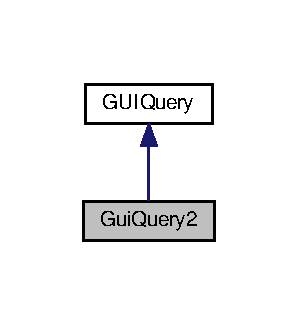
\includegraphics[width=143pt]{classGuiQuery2__inherit__graph}
\end{center}
\end{figure}


Collaboration diagram for Gui\+Query2\+:\nopagebreak
\begin{figure}[H]
\begin{center}
\leavevmode
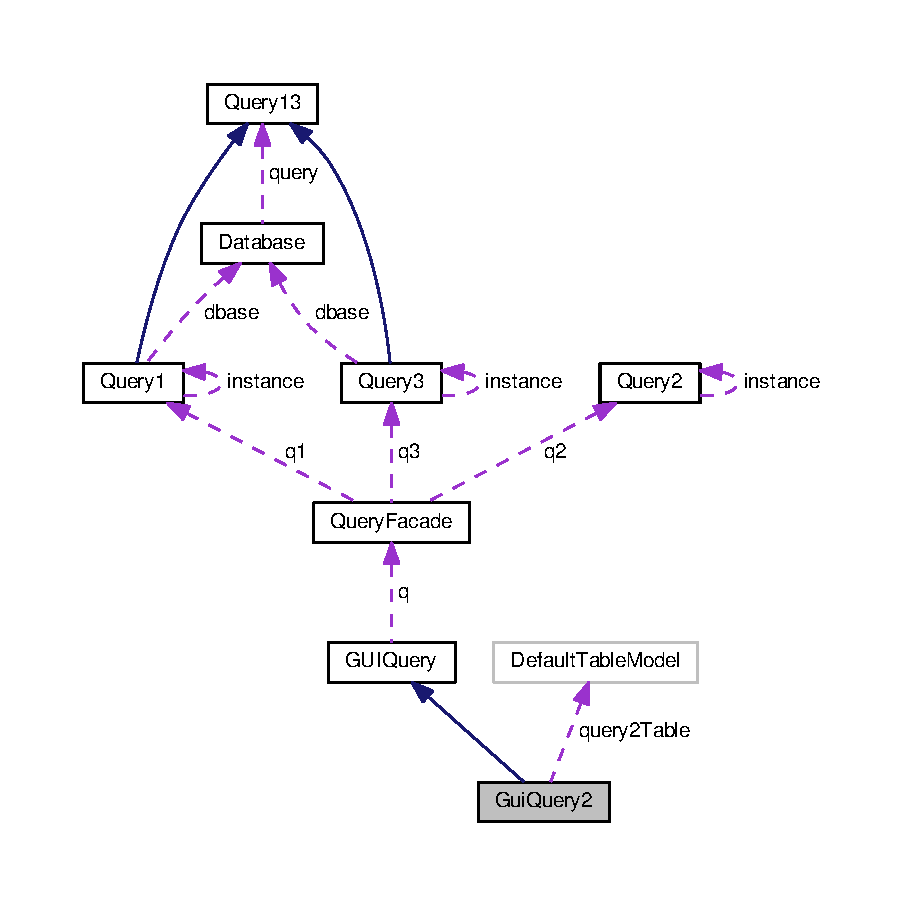
\includegraphics[width=350pt]{classGuiQuery2__coll__graph}
\end{center}
\end{figure}
\subsection*{Public Member Functions}
\begin{DoxyCompactItemize}
\item 
\hyperlink{classGuiQuery2_abf935498d661bd8a8ec951d3238527d7}{Gui\+Query2} (J\+Frame \hyperlink{classGUIQuery_aba988b5bec899d53480a472de7b87dfa}{main\+Frame}, J\+Combo\+Box$<$ String $>$ \hyperlink{classGUIQuery_a0db8bd960b4512cadf9aa40642934680}{queries}, J\+Panel \hyperlink{classGUIQuery_a70e233b1f14874166b7707edebe825d2}{side\+Panel}, J\+Panel \hyperlink{classGUIQuery_a8b4dbf257e0859c597591f072349b75c}{display\+Panel}, \hyperlink{classQueryFacade}{Query\+Facade} q2)
\item 
void \hyperlink{classGuiQuery2_adb51f7db961816ce8f31043affeee2e7}{init\+Query} ()
\item 
void \hyperlink{classGuiQuery2_ad41b33535518a909e7ed9bcd7be271a4}{add\+To\+Panel} ()
\item 
void \hyperlink{classGuiQuery2_a8d5d3771f27c0c86d8af1d8b361218ec}{change} (int i)
\item 
void \hyperlink{classGuiQuery2_a90d0eb0359bc36e9bddcfa6b3308bb85}{change\+Mode} (int i)
\item 
void \hyperlink{classGuiQuery2_af4f531c30a9b1aff5fd0474741611df3}{set\+Query} ()
\end{DoxyCompactItemize}
\subsection*{Private Attributes}
\begin{DoxyCompactItemize}
\item 
int \hyperlink{classGuiQuery2_ac581df0639712a0ef23b6eee49df03e0}{flag} =0
\item 
J\+Label \hyperlink{classGuiQuery2_adb385146a2f0b88b98fa44c95cc4efc5}{title} = new J\+Label(\char`\"{}No. of Publications\char`\"{})
\item 
J\+Text\+Field \hyperlink{classGuiQuery2_aadf0bcfdb4aa2bad406378cf07be0c24}{publk} =new J\+Text\+Field()
\item 
Default\+Table\+Model \hyperlink{classGuiQuery2_a0b3f16b0f92eabbdea82f4abd3ba4377}{query2\+Table} = new Default\+Table\+Model()
\item 
J\+Table \hyperlink{classGuiQuery2_af15c62d5c9199ea2fdf2de7442495c72}{display\+Table} = new J\+Table(\hyperlink{classGuiQuery2_a0b3f16b0f92eabbdea82f4abd3ba4377}{query2\+Table})
\item 
J\+Scroll\+Pane \hyperlink{classGuiQuery2_abba8f10b666db3ea7653c3f6a647fb60}{disp\+Table} = new J\+Scroll\+Pane(\hyperlink{classGuiQuery2_af15c62d5c9199ea2fdf2de7442495c72}{display\+Table})
\item 
J\+Label \hyperlink{classGuiQuery2_ab813118a2db6297717b32f054e5305e9}{warning} = new J\+Label(\char`\"{} \char`\"{})
\item 
J\+Button \hyperlink{classGuiQuery2_a2a63533eaacb408e66da8beb1738b140}{next} = new J\+Button(\char`\"{}N\+E\+XT\char`\"{})
\item 
J\+Button \hyperlink{classGuiQuery2_adb82d5a5b40c916e957bddbca80efb4b}{back} = new J\+Button(\char`\"{}B\+A\+CK\char`\"{})
\item 
Array\+List$<$ \hyperlink{classAuthor}{Author} $>$ \hyperlink{classGuiQuery2_a97d061ff962c9d44c1723bc040c34458}{res} = new Array\+List$<$\hyperlink{classAuthor}{Author}$>$()
\item 
J\+Label \hyperlink{classGuiQuery2_a09768aea9ccb55c5e1d1d9926e2ae048}{total\+Results} = new J\+Label(\char`\"{} \char`\"{})
\end{DoxyCompactItemize}
\subsection*{Additional Inherited Members}


\subsection{Detailed Description}
Creates the \hyperlink{classGUI}{G\+UI} needed for supporting \hyperlink{classQuery2}{Query2} 

\subsection{Constructor \& Destructor Documentation}
\index{Gui\+Query2@{Gui\+Query2}!Gui\+Query2@{Gui\+Query2}}
\index{Gui\+Query2@{Gui\+Query2}!Gui\+Query2@{Gui\+Query2}}
\subsubsection[{\texorpdfstring{Gui\+Query2(\+J\+Frame main\+Frame, J\+Combo\+Box$<$ String $>$ queries, J\+Panel side\+Panel, J\+Panel display\+Panel, Query\+Facade q2)}{GuiQuery2(JFrame mainFrame, JComboBox< String > queries, JPanel sidePanel, JPanel displayPanel, QueryFacade q2)}}]{\setlength{\rightskip}{0pt plus 5cm}Gui\+Query2.\+Gui\+Query2 (
\begin{DoxyParamCaption}
\item[{J\+Frame}]{main\+Frame, }
\item[{J\+Combo\+Box$<$ String $>$}]{queries, }
\item[{J\+Panel}]{side\+Panel, }
\item[{J\+Panel}]{display\+Panel, }
\item[{{\bf Query\+Facade}}]{q2}
\end{DoxyParamCaption}
)\hspace{0.3cm}{\ttfamily [inline]}}\hypertarget{classGuiQuery2_abf935498d661bd8a8ec951d3238527d7}{}\label{classGuiQuery2_abf935498d661bd8a8ec951d3238527d7}

\begin{DoxyCode}
33     \{
34         this.\hyperlink{classGUIQuery_aba988b5bec899d53480a472de7b87dfa}{mainFrame}=\hyperlink{classGUIQuery_aba988b5bec899d53480a472de7b87dfa}{mainFrame};
35         this.\hyperlink{classGUIQuery_a0db8bd960b4512cadf9aa40642934680}{queries}=\hyperlink{classGUIQuery_a0db8bd960b4512cadf9aa40642934680}{queries};
36         this.\hyperlink{classGUIQuery_a70e233b1f14874166b7707edebe825d2}{sidePanel}=\hyperlink{classGUIQuery_a70e233b1f14874166b7707edebe825d2}{sidePanel};
37         this.\hyperlink{classGUIQuery_a8b4dbf257e0859c597591f072349b75c}{displayPanel}=\hyperlink{classGUIQuery_a8b4dbf257e0859c597591f072349b75c}{displayPanel};
38         this.\hyperlink{classGUIQuery_a2a20445d749185552014142b78f3e071}{q}=q2;
39     \}
\end{DoxyCode}


\subsection{Member Function Documentation}
\index{Gui\+Query2@{Gui\+Query2}!add\+To\+Panel@{add\+To\+Panel}}
\index{add\+To\+Panel@{add\+To\+Panel}!Gui\+Query2@{Gui\+Query2}}
\subsubsection[{\texorpdfstring{add\+To\+Panel()}{addToPanel()}}]{\setlength{\rightskip}{0pt plus 5cm}void Gui\+Query2.\+add\+To\+Panel (
\begin{DoxyParamCaption}
{}
\end{DoxyParamCaption}
)\hspace{0.3cm}{\ttfamily [inline]}}\hypertarget{classGuiQuery2_ad41b33535518a909e7ed9bcd7be271a4}{}\label{classGuiQuery2_ad41b33535518a909e7ed9bcd7be271a4}

\begin{DoxyCode}
78     \{
79         \hyperlink{classGUIQuery_a8b4dbf257e0859c597591f072349b75c}{displayPanel}.removeAll();
80         \hyperlink{classGUIQuery_a8b4dbf257e0859c597591f072349b75c}{displayPanel}.add(\hyperlink{classGuiQuery2_a2a63533eaacb408e66da8beb1738b140}{next});
81         \hyperlink{classGUIQuery_a8b4dbf257e0859c597591f072349b75c}{displayPanel}.add(\hyperlink{classGuiQuery2_abba8f10b666db3ea7653c3f6a647fb60}{dispTable});
82         \hyperlink{classGUIQuery_a70e233b1f14874166b7707edebe825d2}{sidePanel}.add(\hyperlink{classGuiQuery2_ab813118a2db6297717b32f054e5305e9}{warning});
83         \hyperlink{classGUIQuery_a70e233b1f14874166b7707edebe825d2}{sidePanel}.add(\hyperlink{classGuiQuery2_adb385146a2f0b88b98fa44c95cc4efc5}{title});
84         \hyperlink{classGUIQuery_a70e233b1f14874166b7707edebe825d2}{sidePanel}.add(\hyperlink{classGUIQuery_a0db8bd960b4512cadf9aa40642934680}{queries});
85         \hyperlink{classGUIQuery_a70e233b1f14874166b7707edebe825d2}{sidePanel}.add(\hyperlink{classGuiQuery2_aadf0bcfdb4aa2bad406378cf07be0c24}{publk});
86         \hyperlink{classGUIQuery_a70e233b1f14874166b7707edebe825d2}{sidePanel}.add(\hyperlink{classGUIQuery_a6580b15e365bc754c1a5ccdd2d58a4bb}{submit});
87         \hyperlink{classGUIQuery_a70e233b1f14874166b7707edebe825d2}{sidePanel}.add(reset);
88         \hyperlink{classGUIQuery_aba988b5bec899d53480a472de7b87dfa}{mainFrame}.revalidate();
89         \hyperlink{classGUIQuery_aba988b5bec899d53480a472de7b87dfa}{mainFrame}.repaint();
90         \hyperlink{classGUIQuery_a8b4dbf257e0859c597591f072349b75c}{displayPanel}.add(\hyperlink{classGuiQuery2_a09768aea9ccb55c5e1d1d9926e2ae048}{totalResults});
91         reset.addActionListener(\textcolor{keyword}{new} ActionListener()\{
92                 \textcolor{keyword}{public} \textcolor{keywordtype}{void} actionPerformed(ActionEvent e)\{
93                     tableWorking=0;
94                     \hyperlink{classGuiQuery2_a0b3f16b0f92eabbdea82f4abd3ba4377}{query2Table}.setRowCount(0);
95                     \hyperlink{classGuiQuery2_aadf0bcfdb4aa2bad406378cf07be0c24}{publk}.setText(\textcolor{stringliteral}{""});
96                     \hyperlink{classGuiQuery2_a09768aea9ccb55c5e1d1d9926e2ae048}{totalResults}.setText(\textcolor{stringliteral}{""});
97                 \}
98             \});
99         
100 
101         \hyperlink{classGuiQuery2_adb82d5a5b40c916e957bddbca80efb4b}{back}.addActionListener(\textcolor{keyword}{new} ActionListener()\{
102             \textcolor{keyword}{public} \textcolor{keywordtype}{void} actionPerformed(ActionEvent e)\{
103 
104             \}
105         \});
106     \}
\end{DoxyCode}
\index{Gui\+Query2@{Gui\+Query2}!change@{change}}
\index{change@{change}!Gui\+Query2@{Gui\+Query2}}
\subsubsection[{\texorpdfstring{change(int i)}{change(int i)}}]{\setlength{\rightskip}{0pt plus 5cm}void Gui\+Query2.\+change (
\begin{DoxyParamCaption}
\item[{int}]{i}
\end{DoxyParamCaption}
)\hspace{0.3cm}{\ttfamily [inline]}}\hypertarget{classGuiQuery2_a8d5d3771f27c0c86d8af1d8b361218ec}{}\label{classGuiQuery2_a8d5d3771f27c0c86d8af1d8b361218ec}

\begin{DoxyCode}
109     \{
110         \hyperlink{classGuiQuery2_ac581df0639712a0ef23b6eee49df03e0}{flag}=i;
111     \}
\end{DoxyCode}
\index{Gui\+Query2@{Gui\+Query2}!change\+Mode@{change\+Mode}}
\index{change\+Mode@{change\+Mode}!Gui\+Query2@{Gui\+Query2}}
\subsubsection[{\texorpdfstring{change\+Mode(int i)}{changeMode(int i)}}]{\setlength{\rightskip}{0pt plus 5cm}void Gui\+Query2.\+change\+Mode (
\begin{DoxyParamCaption}
\item[{int}]{i}
\end{DoxyParamCaption}
)\hspace{0.3cm}{\ttfamily [inline]}}\hypertarget{classGuiQuery2_a90d0eb0359bc36e9bddcfa6b3308bb85}{}\label{classGuiQuery2_a90d0eb0359bc36e9bddcfa6b3308bb85}

\begin{DoxyCode}
113     \{
114         flag2=i;
115     \}
\end{DoxyCode}
\index{Gui\+Query2@{Gui\+Query2}!init\+Query@{init\+Query}}
\index{init\+Query@{init\+Query}!Gui\+Query2@{Gui\+Query2}}
\subsubsection[{\texorpdfstring{init\+Query()}{initQuery()}}]{\setlength{\rightskip}{0pt plus 5cm}void Gui\+Query2.\+init\+Query (
\begin{DoxyParamCaption}
{}
\end{DoxyParamCaption}
)\hspace{0.3cm}{\ttfamily [inline]}}\hypertarget{classGuiQuery2_adb51f7db961816ce8f31043affeee2e7}{}\label{classGuiQuery2_adb51f7db961816ce8f31043affeee2e7}

\begin{DoxyCode}
41                            \{
42         \hyperlink{classGuiQuery2_aadf0bcfdb4aa2bad406378cf07be0c24}{publk}.setBounds(170,80,50,20);
43         \hyperlink{classGuiQuery2_af15c62d5c9199ea2fdf2de7442495c72}{displayTable}.setDefaultEditor(Object.class, null);
44         \hyperlink{classGuiQuery2_abba8f10b666db3ea7653c3f6a647fb60}{dispTable}.setBounds(20,5,910,390);
45         \hyperlink{classGuiQuery2_a0b3f16b0f92eabbdea82f4abd3ba4377}{query2Table}.addColumn(\textcolor{stringliteral}{"S.No."});
46         \hyperlink{classGuiQuery2_a0b3f16b0f92eabbdea82f4abd3ba4377}{query2Table}.addColumn(\textcolor{stringliteral}{"Authors"});
47         \hyperlink{classGuiQuery2_ab813118a2db6297717b32f054e5305e9}{warning}.setFont(\textcolor{keyword}{new} Font(\textcolor{stringliteral}{"Calibri"}, Font.PLAIN, 12));
48         \hyperlink{classGuiQuery2_ab813118a2db6297717b32f054e5305e9}{warning}.setForeground(Color.RED);
49         \hyperlink{classGuiQuery2_ab813118a2db6297717b32f054e5305e9}{warning}.setBounds(30,340,190,20);
50         \hyperlink{classGuiQuery2_a2a63533eaacb408e66da8beb1738b140}{next}.setBounds(840,395,80,40);
51         \hyperlink{classGuiQuery2_a2a63533eaacb408e66da8beb1738b140}{next}.setBackground(Color.RED);
52         \hyperlink{classGuiQuery2_a2a63533eaacb408e66da8beb1738b140}{next}.setFont(\textcolor{keyword}{new} Font(\textcolor{stringliteral}{"Calibri"}, Font.PLAIN, 10));
53         \hyperlink{classGuiQuery2_adb82d5a5b40c916e957bddbca80efb4b}{back}.setBounds(30,395,80,40);
54         \hyperlink{classGuiQuery2_adb82d5a5b40c916e957bddbca80efb4b}{back}.setBackground(Color.BLACK);
55         \hyperlink{classGuiQuery2_adb82d5a5b40c916e957bddbca80efb4b}{back}.setFont(\textcolor{keyword}{new} Font(\textcolor{stringliteral}{"Calibri"}, Font.PLAIN, 10));
56         \hyperlink{classGUIQuery_a6580b15e365bc754c1a5ccdd2d58a4bb}{submit}=\textcolor{keyword}{new} JButton(\textcolor{stringliteral}{"Submit"});
57         reset=\textcolor{keyword}{new} JButton(\textcolor{stringliteral}{"Reset"});
58         \hyperlink{classGUIQuery_a6580b15e365bc754c1a5ccdd2d58a4bb}{submit}.setForeground(Color.WHITE);
59         \hyperlink{classGUIQuery_a6580b15e365bc754c1a5ccdd2d58a4bb}{submit}.setBackground(Color.BLACK);
60         reset.setBackground(Color.RED);
61         \hyperlink{classGUIQuery_a6580b15e365bc754c1a5ccdd2d58a4bb}{submit}.setBounds(30,140,80,30);
62         reset.setBounds(140,140,80,30);
63         \hyperlink{classGUIQuery_a6580b15e365bc754c1a5ccdd2d58a4bb}{submit}.setFont(\textcolor{keyword}{new} Font(\textcolor{stringliteral}{"Calibri"}, Font.PLAIN, 12));
64         reset.setFont(\textcolor{keyword}{new} Font(\textcolor{stringliteral}{"Calibri"}, Font.PLAIN, 12));
65         \hyperlink{classGuiQuery2_a09768aea9ccb55c5e1d1d9926e2ae048}{totalResults}.setFont(\textcolor{keyword}{new} Font(\textcolor{stringliteral}{"Calibri"}, Font.PLAIN, 10));
66         \hyperlink{classGuiQuery2_a09768aea9ccb55c5e1d1d9926e2ae048}{totalResults}.setBounds(515,395,120,30);
67         \hyperlink{classGUIQuery_a0db8bd960b4512cadf9aa40642934680}{queries}.removeItem(\textcolor{stringliteral}{"Queries"});
68         \hyperlink{classGUIQuery_a70e233b1f14874166b7707edebe825d2}{sidePanel}.removeAll();
69         \hyperlink{classGUIQuery_a0db8bd960b4512cadf9aa40642934680}{queries}.setBounds(50,50,100,20);
70         \hyperlink{classGUIQuery_a0db8bd960b4512cadf9aa40642934680}{queries}.setSelectedItem(\textcolor{stringliteral}{"Query 2"});
71         \hyperlink{classGuiQuery2_adb385146a2f0b88b98fa44c95cc4efc5}{title}.setFont(\textcolor{keyword}{new} Font(\textcolor{stringliteral}{"Calibri"}, Font.PLAIN, 12));
72         \hyperlink{classGuiQuery2_adb385146a2f0b88b98fa44c95cc4efc5}{title}.setBounds(30,80,130,30);
73         \hyperlink{classGUIQuery_a0db8bd960b4512cadf9aa40642934680}{queries}.removeItem(\textcolor{stringliteral}{"Queries"});
74         this.\hyperlink{classGuiQuery2_ad41b33535518a909e7ed9bcd7be271a4}{addToPanel}();    
75     \}
\end{DoxyCode}
\index{Gui\+Query2@{Gui\+Query2}!set\+Query@{set\+Query}}
\index{set\+Query@{set\+Query}!Gui\+Query2@{Gui\+Query2}}
\subsubsection[{\texorpdfstring{set\+Query()}{setQuery()}}]{\setlength{\rightskip}{0pt plus 5cm}void Gui\+Query2.\+set\+Query (
\begin{DoxyParamCaption}
{}
\end{DoxyParamCaption}
)\hspace{0.3cm}{\ttfamily [inline]}}\hypertarget{classGuiQuery2_af4f531c30a9b1aff5fd0474741611df3}{}\label{classGuiQuery2_af4f531c30a9b1aff5fd0474741611df3}

\begin{DoxyCode}
117                            \{
118         \hyperlink{classGUIQuery_a6580b15e365bc754c1a5ccdd2d58a4bb}{submit}.addActionListener(\textcolor{keyword}{new} ActionListener()\{
119                 \textcolor{keyword}{public} \textcolor{keywordtype}{void} actionPerformed(ActionEvent e)\{
120                     \hyperlink{classGuiQuery2_a09768aea9ccb55c5e1d1d9926e2ae048}{totalResults}.setText(\textcolor{stringliteral}{" "});
121                     \hyperlink{classGuiQuery2_a0b3f16b0f92eabbdea82f4abd3ba4377}{query2Table}.setRowCount(0);
122                     \textcolor{keywordtype}{int} count=0;
123                     pages=0;
124                     tableWorking=0;
125                     \textcolor{keywordflow}{if}(\hyperlink{classGUIQuery_a2ffddedac70e763f8d4bfc6d24d9a0db}{isInteger}(\hyperlink{classGuiQuery2_aadf0bcfdb4aa2bad406378cf07be0c24}{publk}.getText()))\{
126                         \hyperlink{classGuiQuery2_ab813118a2db6297717b32f054e5305e9}{warning}.setText(\textcolor{stringliteral}{" "});
127                         \hyperlink{classGUIQuery_a2a20445d749185552014142b78f3e071}{q}.\hyperlink{classQueryFacade_ae9371edaf51074aa8ad0c108e492755f}{queryTwoFind}(Integer.parseInt(\hyperlink{classGuiQuery2_aadf0bcfdb4aa2bad406378cf07be0c24}{publk}.getText()));
128                         \textcolor{keywordflow}{if}(\hyperlink{classGUIQuery_a2a20445d749185552014142b78f3e071}{q}.\hyperlink{classQueryFacade_a31b305c90f782be21b5c51692bc0d896}{queryTwoGetCount}()==0)\{
129                             \hyperlink{classGuiQuery2_a09768aea9ccb55c5e1d1d9926e2ae048}{totalResults}.setText(\textcolor{stringliteral}{"No Result Found"});
130                         \} \textcolor{keywordflow}{else}\{
131                             \hyperlink{classGuiQuery2_a09768aea9ccb55c5e1d1d9926e2ae048}{totalResults}.setText(\textcolor{stringliteral}{"Total results = "}+
      \hyperlink{classGUIQuery_a2a20445d749185552014142b78f3e071}{q}.\hyperlink{classQueryFacade_a31b305c90f782be21b5c51692bc0d896}{queryTwoGetCount}());\}
132                         tableWorking=1;
133                         \hyperlink{classAuthor}{Author} a =\hyperlink{classGUIQuery_a2a20445d749185552014142b78f3e071}{q}.\hyperlink{classQueryFacade_a01ab933fe12fac06556af3e2948dbe58}{queryTwoGetData}();
134                         \textcolor{keywordflow}{while}(a!=null && count<20)\{
135                             \hyperlink{classGuiQuery2_a0b3f16b0f92eabbdea82f4abd3ba4377}{query2Table}.addRow(\textcolor{keyword}{new} Object[]\{(count+1),a.
      \hyperlink{classAuthor_a1b7371df3d6db53518e2f3556241c52e}{getName}()\});
136                             a=\hyperlink{classGUIQuery_a2a20445d749185552014142b78f3e071}{q}.\hyperlink{classQueryFacade_a01ab933fe12fac06556af3e2948dbe58}{queryTwoGetData}();
137                             count++;\}
138                         pages=1;
139                     \} \textcolor{keywordflow}{else}\{
140                         \hyperlink{classGuiQuery2_ab813118a2db6297717b32f054e5305e9}{warning}.setText(\textcolor{stringliteral}{"Publications should be numbers"}); \}
141                 \}
142             \}); 
143         \hyperlink{classGuiQuery2_a2a63533eaacb408e66da8beb1738b140}{next}.addActionListener(\textcolor{keyword}{new} ActionListener()\{
144             \textcolor{keyword}{public} \textcolor{keywordtype}{void} actionPerformed(ActionEvent e)\{
145                 \textcolor{keywordflow}{if}(tableWorking==1)\{
146                     \hyperlink{classAuthor}{Author} a =\hyperlink{classGUIQuery_a2a20445d749185552014142b78f3e071}{q}.\hyperlink{classQueryFacade_a01ab933fe12fac06556af3e2948dbe58}{queryTwoGetData}();
147                     \textcolor{keywordflow}{if}(a!=null)\{    
148                         \textcolor{keywordtype}{int} count=0;
149                         \hyperlink{classGuiQuery2_a0b3f16b0f92eabbdea82f4abd3ba4377}{query2Table}.setRowCount(0);
150                         \textcolor{keywordflow}{while}(a!=null && count<20)\{
151                             \hyperlink{classGuiQuery2_a0b3f16b0f92eabbdea82f4abd3ba4377}{query2Table}.addRow(\textcolor{keyword}{new} Object[]\{(pages*20)+(count+1),a.
      \hyperlink{classAuthor_a1b7371df3d6db53518e2f3556241c52e}{getName}()\});
152                             count++;
153                             \textcolor{keywordflow}{if}(count<20)\{
154                             a=\hyperlink{classGUIQuery_a2a20445d749185552014142b78f3e071}{q}.\hyperlink{classQueryFacade_a01ab933fe12fac06556af3e2948dbe58}{queryTwoGetData}();\} 
155                         \}
156                         pages+=1;\}
157                 \} \textcolor{keywordflow}{else}\{
158                     tableWorking=0;\}
159             \}
160         \});
161     \}
\end{DoxyCode}


\subsection{Member Data Documentation}
\index{Gui\+Query2@{Gui\+Query2}!back@{back}}
\index{back@{back}!Gui\+Query2@{Gui\+Query2}}
\subsubsection[{\texorpdfstring{back}{back}}]{\setlength{\rightskip}{0pt plus 5cm}J\+Button Gui\+Query2.\+back = new J\+Button(\char`\"{}B\+A\+CK\char`\"{})\hspace{0.3cm}{\ttfamily [private]}}\hypertarget{classGuiQuery2_adb82d5a5b40c916e957bddbca80efb4b}{}\label{classGuiQuery2_adb82d5a5b40c916e957bddbca80efb4b}
\index{Gui\+Query2@{Gui\+Query2}!display\+Table@{display\+Table}}
\index{display\+Table@{display\+Table}!Gui\+Query2@{Gui\+Query2}}
\subsubsection[{\texorpdfstring{display\+Table}{displayTable}}]{\setlength{\rightskip}{0pt plus 5cm}J\+Table Gui\+Query2.\+display\+Table = new J\+Table({\bf query2\+Table})\hspace{0.3cm}{\ttfamily [private]}}\hypertarget{classGuiQuery2_af15c62d5c9199ea2fdf2de7442495c72}{}\label{classGuiQuery2_af15c62d5c9199ea2fdf2de7442495c72}
\index{Gui\+Query2@{Gui\+Query2}!disp\+Table@{disp\+Table}}
\index{disp\+Table@{disp\+Table}!Gui\+Query2@{Gui\+Query2}}
\subsubsection[{\texorpdfstring{disp\+Table}{dispTable}}]{\setlength{\rightskip}{0pt plus 5cm}J\+Scroll\+Pane Gui\+Query2.\+disp\+Table = new J\+Scroll\+Pane({\bf display\+Table})\hspace{0.3cm}{\ttfamily [private]}}\hypertarget{classGuiQuery2_abba8f10b666db3ea7653c3f6a647fb60}{}\label{classGuiQuery2_abba8f10b666db3ea7653c3f6a647fb60}
\index{Gui\+Query2@{Gui\+Query2}!flag@{flag}}
\index{flag@{flag}!Gui\+Query2@{Gui\+Query2}}
\subsubsection[{\texorpdfstring{flag}{flag}}]{\setlength{\rightskip}{0pt plus 5cm}int Gui\+Query2.\+flag =0\hspace{0.3cm}{\ttfamily [private]}}\hypertarget{classGuiQuery2_ac581df0639712a0ef23b6eee49df03e0}{}\label{classGuiQuery2_ac581df0639712a0ef23b6eee49df03e0}
\index{Gui\+Query2@{Gui\+Query2}!next@{next}}
\index{next@{next}!Gui\+Query2@{Gui\+Query2}}
\subsubsection[{\texorpdfstring{next}{next}}]{\setlength{\rightskip}{0pt plus 5cm}J\+Button Gui\+Query2.\+next = new J\+Button(\char`\"{}N\+E\+XT\char`\"{})\hspace{0.3cm}{\ttfamily [private]}}\hypertarget{classGuiQuery2_a2a63533eaacb408e66da8beb1738b140}{}\label{classGuiQuery2_a2a63533eaacb408e66da8beb1738b140}
\index{Gui\+Query2@{Gui\+Query2}!publk@{publk}}
\index{publk@{publk}!Gui\+Query2@{Gui\+Query2}}
\subsubsection[{\texorpdfstring{publk}{publk}}]{\setlength{\rightskip}{0pt plus 5cm}J\+Text\+Field Gui\+Query2.\+publk =new J\+Text\+Field()\hspace{0.3cm}{\ttfamily [private]}}\hypertarget{classGuiQuery2_aadf0bcfdb4aa2bad406378cf07be0c24}{}\label{classGuiQuery2_aadf0bcfdb4aa2bad406378cf07be0c24}
\index{Gui\+Query2@{Gui\+Query2}!query2\+Table@{query2\+Table}}
\index{query2\+Table@{query2\+Table}!Gui\+Query2@{Gui\+Query2}}
\subsubsection[{\texorpdfstring{query2\+Table}{query2Table}}]{\setlength{\rightskip}{0pt plus 5cm}Default\+Table\+Model Gui\+Query2.\+query2\+Table = new Default\+Table\+Model()\hspace{0.3cm}{\ttfamily [private]}}\hypertarget{classGuiQuery2_a0b3f16b0f92eabbdea82f4abd3ba4377}{}\label{classGuiQuery2_a0b3f16b0f92eabbdea82f4abd3ba4377}
\index{Gui\+Query2@{Gui\+Query2}!res@{res}}
\index{res@{res}!Gui\+Query2@{Gui\+Query2}}
\subsubsection[{\texorpdfstring{res}{res}}]{\setlength{\rightskip}{0pt plus 5cm}Array\+List$<${\bf Author}$>$ Gui\+Query2.\+res = new Array\+List$<${\bf Author}$>$()\hspace{0.3cm}{\ttfamily [private]}}\hypertarget{classGuiQuery2_a97d061ff962c9d44c1723bc040c34458}{}\label{classGuiQuery2_a97d061ff962c9d44c1723bc040c34458}
\index{Gui\+Query2@{Gui\+Query2}!title@{title}}
\index{title@{title}!Gui\+Query2@{Gui\+Query2}}
\subsubsection[{\texorpdfstring{title}{title}}]{\setlength{\rightskip}{0pt plus 5cm}J\+Label Gui\+Query2.\+title = new J\+Label(\char`\"{}No. of Publications\char`\"{})\hspace{0.3cm}{\ttfamily [private]}}\hypertarget{classGuiQuery2_adb385146a2f0b88b98fa44c95cc4efc5}{}\label{classGuiQuery2_adb385146a2f0b88b98fa44c95cc4efc5}
\index{Gui\+Query2@{Gui\+Query2}!total\+Results@{total\+Results}}
\index{total\+Results@{total\+Results}!Gui\+Query2@{Gui\+Query2}}
\subsubsection[{\texorpdfstring{total\+Results}{totalResults}}]{\setlength{\rightskip}{0pt plus 5cm}J\+Label Gui\+Query2.\+total\+Results = new J\+Label(\char`\"{} \char`\"{})\hspace{0.3cm}{\ttfamily [private]}}\hypertarget{classGuiQuery2_a09768aea9ccb55c5e1d1d9926e2ae048}{}\label{classGuiQuery2_a09768aea9ccb55c5e1d1d9926e2ae048}
\index{Gui\+Query2@{Gui\+Query2}!warning@{warning}}
\index{warning@{warning}!Gui\+Query2@{Gui\+Query2}}
\subsubsection[{\texorpdfstring{warning}{warning}}]{\setlength{\rightskip}{0pt plus 5cm}J\+Label Gui\+Query2.\+warning = new J\+Label(\char`\"{} \char`\"{})\hspace{0.3cm}{\ttfamily [private]}}\hypertarget{classGuiQuery2_ab813118a2db6297717b32f054e5305e9}{}\label{classGuiQuery2_ab813118a2db6297717b32f054e5305e9}


The documentation for this class was generated from the following file\+:\begin{DoxyCompactItemize}
\item 
\hyperlink{GuiQuery2_8java}{Gui\+Query2.\+java}\end{DoxyCompactItemize}

\hypertarget{classGuiQuery3}{}\section{Gui\+Query3 Class Reference}
\label{classGuiQuery3}\index{Gui\+Query3@{Gui\+Query3}}


Inheritance diagram for Gui\+Query3\+:\nopagebreak
\begin{figure}[H]
\begin{center}
\leavevmode
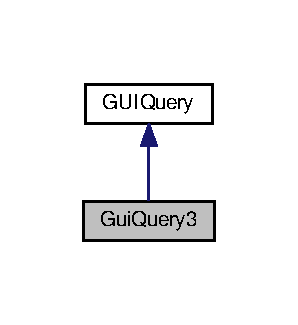
\includegraphics[width=143pt]{classGuiQuery3__inherit__graph}
\end{center}
\end{figure}


Collaboration diagram for Gui\+Query3\+:\nopagebreak
\begin{figure}[H]
\begin{center}
\leavevmode
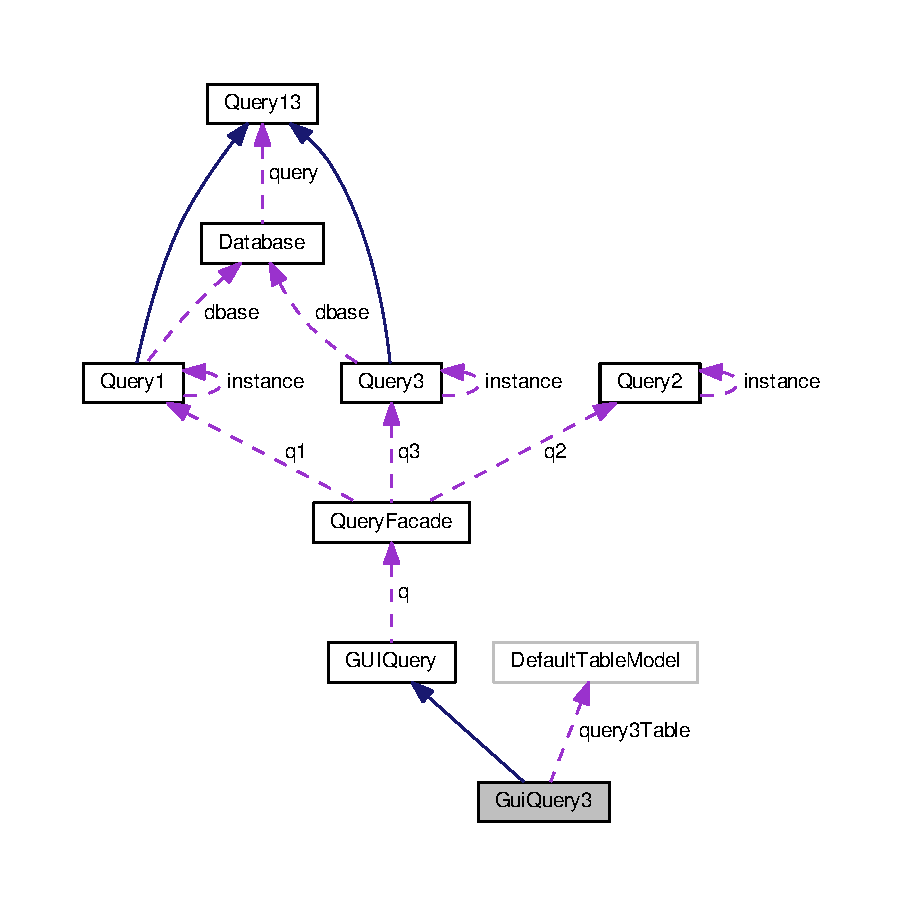
\includegraphics[width=350pt]{classGuiQuery3__coll__graph}
\end{center}
\end{figure}
\subsection*{Public Member Functions}
\begin{DoxyCompactItemize}
\item 
\hyperlink{classGuiQuery3_a6abf4556ef8602ed3f6151439965841f}{Gui\+Query3} (J\+Frame \hyperlink{classGUIQuery_aba988b5bec899d53480a472de7b87dfa}{main\+Frame}, J\+Combo\+Box$<$ String $>$ \hyperlink{classGUIQuery_a0db8bd960b4512cadf9aa40642934680}{queries}, J\+Panel \hyperlink{classGUIQuery_a70e233b1f14874166b7707edebe825d2}{side\+Panel}, J\+Panel \hyperlink{classGUIQuery_a8b4dbf257e0859c597591f072349b75c}{display\+Panel}, \hyperlink{classQueryFacade}{Query\+Facade} q3)
\item 
void \hyperlink{classGuiQuery3_a6d7a0d2ab524cd98ed76495e80f810cc}{init\+Query} ()
\item 
void \hyperlink{classGuiQuery3_afba341da96f35e822f6da33e9eca9941}{set\+Query} ()
\end{DoxyCompactItemize}
\subsection*{Private Attributes}
\begin{DoxyCompactItemize}
\item 
int \hyperlink{classGuiQuery3_acf9c75dae1db9c0c40a25d88137cb372}{flag} =0
\item 
J\+Label \hyperlink{classGuiQuery3_a7e581a0af7c5a7aafe78127499af4ea6}{title} = new J\+Label(\char`\"{}Name of \hyperlink{classAuthor}{Author}\char`\"{})
\item 
J\+Label \hyperlink{classGuiQuery3_a9edee5c70fc9ce109601436c5556675f}{title1} = new J\+Label(\char`\"{}Prediction after year\char`\"{})
\item 
J\+Text\+Field \hyperlink{classGuiQuery3_aa3273681bd3a7b3b44b36fd2b2fddcd4}{auth\+Name} =new J\+Text\+Field()
\item 
J\+Text\+Field \hyperlink{classGuiQuery3_afedb6af40be4ff198922c85bbe94716f}{pred\+Year} =new J\+Text\+Field()
\item 
Default\+Table\+Model \hyperlink{classGuiQuery3_a8273c6d7086d34e6f91fc9721af410d9}{query3\+Table} = new Default\+Table\+Model()
\item 
J\+Table \hyperlink{classGuiQuery3_a868222082fb015a87bac64a3c671389d}{display\+Table} = new J\+Table(\hyperlink{classGuiQuery3_a8273c6d7086d34e6f91fc9721af410d9}{query3\+Table})
\item 
J\+Scroll\+Pane \hyperlink{classGuiQuery3_acd36b4ab5f212d4a4fae20d4a8ffcba4}{disp\+Table} = new J\+Scroll\+Pane(\hyperlink{classGuiQuery3_a868222082fb015a87bac64a3c671389d}{display\+Table})
\item 
J\+Label \hyperlink{classGuiQuery3_a2452813fd6a5ff8c945ccadde7ad4853}{warning} = new J\+Label(\char`\"{} \char`\"{})
\item 
J\+Button \hyperlink{classGuiQuery3_a4d7e8b050499e731a78c43d9c41782e6}{next} = new J\+Button(\char`\"{}N\+E\+XT\char`\"{})
\item 
J\+Button \hyperlink{classGuiQuery3_aa545da5c2e8152ea18c51297734a6910}{back} = new J\+Button(\char`\"{}B\+A\+CK\char`\"{})
\end{DoxyCompactItemize}
\subsection*{Additional Inherited Members}


\subsection{Detailed Description}
Creates the \hyperlink{classGUI}{G\+UI} needed for supporting \hyperlink{classQuery3}{Query3} 

\subsection{Constructor \& Destructor Documentation}
\index{Gui\+Query3@{Gui\+Query3}!Gui\+Query3@{Gui\+Query3}}
\index{Gui\+Query3@{Gui\+Query3}!Gui\+Query3@{Gui\+Query3}}
\subsubsection[{\texorpdfstring{Gui\+Query3(\+J\+Frame main\+Frame, J\+Combo\+Box$<$ String $>$ queries, J\+Panel side\+Panel, J\+Panel display\+Panel, Query\+Facade q3)}{GuiQuery3(JFrame mainFrame, JComboBox< String > queries, JPanel sidePanel, JPanel displayPanel, QueryFacade q3)}}]{\setlength{\rightskip}{0pt plus 5cm}Gui\+Query3.\+Gui\+Query3 (
\begin{DoxyParamCaption}
\item[{J\+Frame}]{main\+Frame, }
\item[{J\+Combo\+Box$<$ String $>$}]{queries, }
\item[{J\+Panel}]{side\+Panel, }
\item[{J\+Panel}]{display\+Panel, }
\item[{{\bf Query\+Facade}}]{q3}
\end{DoxyParamCaption}
)\hspace{0.3cm}{\ttfamily [inline]}}\hypertarget{classGuiQuery3_a6abf4556ef8602ed3f6151439965841f}{}\label{classGuiQuery3_a6abf4556ef8602ed3f6151439965841f}

\begin{DoxyCode}
33     \{
34         this.\hyperlink{classGUIQuery_aba988b5bec899d53480a472de7b87dfa}{mainFrame}=\hyperlink{classGUIQuery_aba988b5bec899d53480a472de7b87dfa}{mainFrame};
35         this.\hyperlink{classGUIQuery_a0db8bd960b4512cadf9aa40642934680}{queries}=\hyperlink{classGUIQuery_a0db8bd960b4512cadf9aa40642934680}{queries};
36         this.\hyperlink{classGUIQuery_a70e233b1f14874166b7707edebe825d2}{sidePanel}=\hyperlink{classGUIQuery_a70e233b1f14874166b7707edebe825d2}{sidePanel};
37         this.\hyperlink{classGUIQuery_a8b4dbf257e0859c597591f072349b75c}{displayPanel}=\hyperlink{classGUIQuery_a8b4dbf257e0859c597591f072349b75c}{displayPanel};
38         this.\hyperlink{classGUIQuery_a2a20445d749185552014142b78f3e071}{q}=q3;
39     \}
\end{DoxyCode}


\subsection{Member Function Documentation}
\index{Gui\+Query3@{Gui\+Query3}!init\+Query@{init\+Query}}
\index{init\+Query@{init\+Query}!Gui\+Query3@{Gui\+Query3}}
\subsubsection[{\texorpdfstring{init\+Query()}{initQuery()}}]{\setlength{\rightskip}{0pt plus 5cm}void Gui\+Query3.\+init\+Query (
\begin{DoxyParamCaption}
{}
\end{DoxyParamCaption}
)\hspace{0.3cm}{\ttfamily [inline]}}\hypertarget{classGuiQuery3_a6d7a0d2ab524cd98ed76495e80f810cc}{}\label{classGuiQuery3_a6d7a0d2ab524cd98ed76495e80f810cc}

\begin{DoxyCode}
42     \{
43         \hyperlink{classGUIQuery_a6580b15e365bc754c1a5ccdd2d58a4bb}{submit}=\textcolor{keyword}{new} JButton(\textcolor{stringliteral}{"Submit"});
44         reset=\textcolor{keyword}{new} JButton(\textcolor{stringliteral}{"Reset"});
45         \hyperlink{classGUIQuery_a6580b15e365bc754c1a5ccdd2d58a4bb}{submit}.setBackground(Color.BLACK);
46         reset.setBackground(Color.RED);
47         \hyperlink{classGuiQuery3_a7e581a0af7c5a7aafe78127499af4ea6}{title}.setFont(\textcolor{keyword}{new} Font(\textcolor{stringliteral}{"Calibri"}, Font.PLAIN, 12));
48         \hyperlink{classGuiQuery3_a7e581a0af7c5a7aafe78127499af4ea6}{title}.setBounds(30,80,130,20);
49         \hyperlink{classGuiQuery3_a9edee5c70fc9ce109601436c5556675f}{title1}.setFont(\textcolor{keyword}{new} Font(\textcolor{stringliteral}{"Calibri"}, Font.PLAIN, 12));
50         \hyperlink{classGuiQuery3_a9edee5c70fc9ce109601436c5556675f}{title1}.setBounds(30,105,130,20);
51         \hyperlink{classGuiQuery3_aa3273681bd3a7b3b44b36fd2b2fddcd4}{authName}.setBounds(170,80,50,20);
52         \hyperlink{classGuiQuery3_afedb6af40be4ff198922c85bbe94716f}{predYear}.setBounds(170,105,50,20);
53         \hyperlink{classGUIQuery_a6580b15e365bc754c1a5ccdd2d58a4bb}{submit}.setForeground(Color.WHITE);
54         \hyperlink{classGUIQuery_a6580b15e365bc754c1a5ccdd2d58a4bb}{submit}.setBounds(30,155,80,30);
55         reset.setBounds(140,155,80,30);
56         \hyperlink{classGUIQuery_a6580b15e365bc754c1a5ccdd2d58a4bb}{submit}.setFont(\textcolor{keyword}{new} Font(\textcolor{stringliteral}{"Calibri"}, Font.PLAIN, 12));
57         reset.setFont(\textcolor{keyword}{new} Font(\textcolor{stringliteral}{"Calibri"}, Font.PLAIN, 12));
58         \hyperlink{classGuiQuery3_a868222082fb015a87bac64a3c671389d}{displayTable}.setDefaultEditor(Object.class, null);
59         \hyperlink{classGuiQuery3_acd36b4ab5f212d4a4fae20d4a8ffcba4}{dispTable}.setBounds(20,5,910,390);
60         \hyperlink{classGuiQuery3_a8273c6d7086d34e6f91fc9721af410d9}{query3Table}.addColumn(\textcolor{stringliteral}{"S.No."});
61         \hyperlink{classGuiQuery3_a8273c6d7086d34e6f91fc9721af410d9}{query3Table}.addColumn(\textcolor{stringliteral}{"Authors"});
62         \hyperlink{classGuiQuery3_a8273c6d7086d34e6f91fc9721af410d9}{query3Table}.addColumn(\textcolor{stringliteral}{"Predicted Value"});
63         \hyperlink{classGuiQuery3_a2452813fd6a5ff8c945ccadde7ad4853}{warning}.setForeground(Color.RED);
64         \hyperlink{classGuiQuery3_a2452813fd6a5ff8c945ccadde7ad4853}{warning}.setBounds(30,340,190,20);
65         \hyperlink{classGuiQuery3_a2452813fd6a5ff8c945ccadde7ad4853}{warning}.setFont(\textcolor{keyword}{new} Font(\textcolor{stringliteral}{"Calibri"}, Font.PLAIN, 12));
66         \hyperlink{classGuiQuery3_a4d7e8b050499e731a78c43d9c41782e6}{next}.setBounds(540,335,80,40);
67         \hyperlink{classGuiQuery3_a4d7e8b050499e731a78c43d9c41782e6}{next}.setBackground(Color.RED);
68         \hyperlink{classGuiQuery3_a4d7e8b050499e731a78c43d9c41782e6}{next}.setFont(\textcolor{keyword}{new} Font(\textcolor{stringliteral}{"Calibri"}, Font.PLAIN, 10));
69         \hyperlink{classGuiQuery3_aa545da5c2e8152ea18c51297734a6910}{back}.setBounds(30,335,80,40);
70         \hyperlink{classGuiQuery3_aa545da5c2e8152ea18c51297734a6910}{back}.setBackground(Color.BLACK);
71         \hyperlink{classGuiQuery3_aa545da5c2e8152ea18c51297734a6910}{back}.setFont(\textcolor{keyword}{new} Font(\textcolor{stringliteral}{"Calibri"}, Font.PLAIN, 10));
72     \}
\end{DoxyCode}
\index{Gui\+Query3@{Gui\+Query3}!set\+Query@{set\+Query}}
\index{set\+Query@{set\+Query}!Gui\+Query3@{Gui\+Query3}}
\subsubsection[{\texorpdfstring{set\+Query()}{setQuery()}}]{\setlength{\rightskip}{0pt plus 5cm}void Gui\+Query3.\+set\+Query (
\begin{DoxyParamCaption}
{}
\end{DoxyParamCaption}
)\hspace{0.3cm}{\ttfamily [inline]}}\hypertarget{classGuiQuery3_afba341da96f35e822f6da33e9eca9941}{}\label{classGuiQuery3_afba341da96f35e822f6da33e9eca9941}

\begin{DoxyCode}
75     \{
76         \hyperlink{classGUIQuery_a0db8bd960b4512cadf9aa40642934680}{queries}.removeItem(\textcolor{stringliteral}{"Queries"});
77         \hyperlink{classGUIQuery_a70e233b1f14874166b7707edebe825d2}{sidePanel}.removeAll();
78         \hyperlink{classGUIQuery_a0db8bd960b4512cadf9aa40642934680}{queries}.setBounds(50,50,100,20);
79         \hyperlink{classGUIQuery_a0db8bd960b4512cadf9aa40642934680}{queries}.setSelectedItem(\textcolor{stringliteral}{"Query 3"});
80         \hyperlink{classGUIQuery_a0db8bd960b4512cadf9aa40642934680}{queries}.removeItem(\textcolor{stringliteral}{"Queries"});
81         \hyperlink{classGUIQuery_a8b4dbf257e0859c597591f072349b75c}{displayPanel}.removeAll();
82         \hyperlink{classGUIQuery_a8b4dbf257e0859c597591f072349b75c}{displayPanel}.add(\hyperlink{classGuiQuery3_acd36b4ab5f212d4a4fae20d4a8ffcba4}{dispTable});
83         \hyperlink{classGUIQuery_a70e233b1f14874166b7707edebe825d2}{sidePanel}.add(\hyperlink{classGuiQuery3_a2452813fd6a5ff8c945ccadde7ad4853}{warning});
84         \hyperlink{classGUIQuery_a70e233b1f14874166b7707edebe825d2}{sidePanel}.add(\hyperlink{classGuiQuery3_a7e581a0af7c5a7aafe78127499af4ea6}{title});
85         \hyperlink{classGUIQuery_a70e233b1f14874166b7707edebe825d2}{sidePanel}.add(\hyperlink{classGUIQuery_a0db8bd960b4512cadf9aa40642934680}{queries});
86         \hyperlink{classGUIQuery_a70e233b1f14874166b7707edebe825d2}{sidePanel}.add(\hyperlink{classGuiQuery3_a9edee5c70fc9ce109601436c5556675f}{title1});
87         \hyperlink{classGUIQuery_a70e233b1f14874166b7707edebe825d2}{sidePanel}.add(\hyperlink{classGuiQuery3_afedb6af40be4ff198922c85bbe94716f}{predYear});
88         \hyperlink{classGUIQuery_a70e233b1f14874166b7707edebe825d2}{sidePanel}.add(\hyperlink{classGuiQuery3_aa3273681bd3a7b3b44b36fd2b2fddcd4}{authName});
89         \hyperlink{classGUIQuery_a70e233b1f14874166b7707edebe825d2}{sidePanel}.add(\hyperlink{classGUIQuery_a6580b15e365bc754c1a5ccdd2d58a4bb}{submit});
90         \hyperlink{classGUIQuery_a70e233b1f14874166b7707edebe825d2}{sidePanel}.add(reset);
91         \hyperlink{classGUIQuery_aba988b5bec899d53480a472de7b87dfa}{mainFrame}.revalidate();
92         \hyperlink{classGUIQuery_aba988b5bec899d53480a472de7b87dfa}{mainFrame}.repaint();
93         \hyperlink{classGUIQuery_a6580b15e365bc754c1a5ccdd2d58a4bb}{submit}.addActionListener(\textcolor{keyword}{new} ActionListener()\{
94                 \textcolor{keyword}{public} \textcolor{keywordtype}{void} actionPerformed(ActionEvent e)
95                 \{
96                     \hyperlink{classGuiQuery3_a8273c6d7086d34e6f91fc9721af410d9}{query3Table}.setRowCount(0);
97                     tableWorking=0;
98                     \textcolor{keywordflow}{if}(\hyperlink{classGuiQuery3_aa3273681bd3a7b3b44b36fd2b2fddcd4}{authName}.getText().length()==0)\{
99                         \hyperlink{classGuiQuery3_a2452813fd6a5ff8c945ccadde7ad4853}{warning}.setText(\textcolor{stringliteral}{"Author Name can not be empty"});
100                     \} \textcolor{keywordflow}{else} \{
101                         \textcolor{keywordflow}{if}(\hyperlink{classGUIQuery_a2ffddedac70e763f8d4bfc6d24d9a0db}{isInteger}(\hyperlink{classGuiQuery3_afedb6af40be4ff198922c85bbe94716f}{predYear}.getText())) \{
102                             \hyperlink{classGuiQuery3_a2452813fd6a5ff8c945ccadde7ad4853}{warning}.setText(\textcolor{stringliteral}{" "});
103                             \hyperlink{classGUIQuery_a2a20445d749185552014142b78f3e071}{q}.\hyperlink{classQueryFacade_afa8c14d931ca1708a09ae94bd435504a}{queryThreeFind}(Integer.parseInt(
      \hyperlink{classGuiQuery3_afedb6af40be4ff198922c85bbe94716f}{predYear}.getText()),\hyperlink{classGuiQuery3_aa3273681bd3a7b3b44b36fd2b2fddcd4}{authName}.getText());
104                             tableWorking=1;
105                             \textcolor{keywordtype}{double} a =\hyperlink{classGUIQuery_a2a20445d749185552014142b78f3e071}{q}.\hyperlink{classQueryFacade_a394c9283bc3bdfc0060a5eabece24782}{queryThreeGetData}();
106                             \textcolor{keywordflow}{if}(a==-1.0)\{
107                                 \hyperlink{classGuiQuery3_a2452813fd6a5ff8c945ccadde7ad4853}{warning}.setText(\textcolor{stringliteral}{"No result Found"});
108                             \} \textcolor{keywordflow}{else}\{
109                             \hyperlink{classGuiQuery3_a8273c6d7086d34e6f91fc9721af410d9}{query3Table}.addRow(\textcolor{keyword}{new} Object[]\{1,
      \hyperlink{classGuiQuery3_aa3273681bd3a7b3b44b36fd2b2fddcd4}{authName}.getText(),a\});\}
110                         \}
111                         \textcolor{keywordflow}{else} \{
112                             \hyperlink{classGuiQuery3_a2452813fd6a5ff8c945ccadde7ad4853}{warning}.setText(\textcolor{stringliteral}{"Year field should be numbers"});\}
113                     \}
114                 \}
115             \});
116         reset.addActionListener(\textcolor{keyword}{new} ActionListener()\{
117                 \textcolor{keyword}{public} \textcolor{keywordtype}{void} actionPerformed(ActionEvent e)
118                 \{
119                     \hyperlink{classGuiQuery3_aa3273681bd3a7b3b44b36fd2b2fddcd4}{authName}.setText(\textcolor{stringliteral}{""});
120                     \hyperlink{classGuiQuery3_afedb6af40be4ff198922c85bbe94716f}{predYear}.setText(\textcolor{stringliteral}{""});
121                 \}
122             \});
123     \}
\end{DoxyCode}


\subsection{Member Data Documentation}
\index{Gui\+Query3@{Gui\+Query3}!auth\+Name@{auth\+Name}}
\index{auth\+Name@{auth\+Name}!Gui\+Query3@{Gui\+Query3}}
\subsubsection[{\texorpdfstring{auth\+Name}{authName}}]{\setlength{\rightskip}{0pt plus 5cm}J\+Text\+Field Gui\+Query3.\+auth\+Name =new J\+Text\+Field()\hspace{0.3cm}{\ttfamily [private]}}\hypertarget{classGuiQuery3_aa3273681bd3a7b3b44b36fd2b2fddcd4}{}\label{classGuiQuery3_aa3273681bd3a7b3b44b36fd2b2fddcd4}
\index{Gui\+Query3@{Gui\+Query3}!back@{back}}
\index{back@{back}!Gui\+Query3@{Gui\+Query3}}
\subsubsection[{\texorpdfstring{back}{back}}]{\setlength{\rightskip}{0pt plus 5cm}J\+Button Gui\+Query3.\+back = new J\+Button(\char`\"{}B\+A\+CK\char`\"{})\hspace{0.3cm}{\ttfamily [private]}}\hypertarget{classGuiQuery3_aa545da5c2e8152ea18c51297734a6910}{}\label{classGuiQuery3_aa545da5c2e8152ea18c51297734a6910}
\index{Gui\+Query3@{Gui\+Query3}!display\+Table@{display\+Table}}
\index{display\+Table@{display\+Table}!Gui\+Query3@{Gui\+Query3}}
\subsubsection[{\texorpdfstring{display\+Table}{displayTable}}]{\setlength{\rightskip}{0pt plus 5cm}J\+Table Gui\+Query3.\+display\+Table = new J\+Table({\bf query3\+Table})\hspace{0.3cm}{\ttfamily [private]}}\hypertarget{classGuiQuery3_a868222082fb015a87bac64a3c671389d}{}\label{classGuiQuery3_a868222082fb015a87bac64a3c671389d}
\index{Gui\+Query3@{Gui\+Query3}!disp\+Table@{disp\+Table}}
\index{disp\+Table@{disp\+Table}!Gui\+Query3@{Gui\+Query3}}
\subsubsection[{\texorpdfstring{disp\+Table}{dispTable}}]{\setlength{\rightskip}{0pt plus 5cm}J\+Scroll\+Pane Gui\+Query3.\+disp\+Table = new J\+Scroll\+Pane({\bf display\+Table})\hspace{0.3cm}{\ttfamily [private]}}\hypertarget{classGuiQuery3_acd36b4ab5f212d4a4fae20d4a8ffcba4}{}\label{classGuiQuery3_acd36b4ab5f212d4a4fae20d4a8ffcba4}
\index{Gui\+Query3@{Gui\+Query3}!flag@{flag}}
\index{flag@{flag}!Gui\+Query3@{Gui\+Query3}}
\subsubsection[{\texorpdfstring{flag}{flag}}]{\setlength{\rightskip}{0pt plus 5cm}int Gui\+Query3.\+flag =0\hspace{0.3cm}{\ttfamily [private]}}\hypertarget{classGuiQuery3_acf9c75dae1db9c0c40a25d88137cb372}{}\label{classGuiQuery3_acf9c75dae1db9c0c40a25d88137cb372}
\index{Gui\+Query3@{Gui\+Query3}!next@{next}}
\index{next@{next}!Gui\+Query3@{Gui\+Query3}}
\subsubsection[{\texorpdfstring{next}{next}}]{\setlength{\rightskip}{0pt plus 5cm}J\+Button Gui\+Query3.\+next = new J\+Button(\char`\"{}N\+E\+XT\char`\"{})\hspace{0.3cm}{\ttfamily [private]}}\hypertarget{classGuiQuery3_a4d7e8b050499e731a78c43d9c41782e6}{}\label{classGuiQuery3_a4d7e8b050499e731a78c43d9c41782e6}
\index{Gui\+Query3@{Gui\+Query3}!pred\+Year@{pred\+Year}}
\index{pred\+Year@{pred\+Year}!Gui\+Query3@{Gui\+Query3}}
\subsubsection[{\texorpdfstring{pred\+Year}{predYear}}]{\setlength{\rightskip}{0pt plus 5cm}J\+Text\+Field Gui\+Query3.\+pred\+Year =new J\+Text\+Field()\hspace{0.3cm}{\ttfamily [private]}}\hypertarget{classGuiQuery3_afedb6af40be4ff198922c85bbe94716f}{}\label{classGuiQuery3_afedb6af40be4ff198922c85bbe94716f}
\index{Gui\+Query3@{Gui\+Query3}!query3\+Table@{query3\+Table}}
\index{query3\+Table@{query3\+Table}!Gui\+Query3@{Gui\+Query3}}
\subsubsection[{\texorpdfstring{query3\+Table}{query3Table}}]{\setlength{\rightskip}{0pt plus 5cm}Default\+Table\+Model Gui\+Query3.\+query3\+Table = new Default\+Table\+Model()\hspace{0.3cm}{\ttfamily [private]}}\hypertarget{classGuiQuery3_a8273c6d7086d34e6f91fc9721af410d9}{}\label{classGuiQuery3_a8273c6d7086d34e6f91fc9721af410d9}
\index{Gui\+Query3@{Gui\+Query3}!title@{title}}
\index{title@{title}!Gui\+Query3@{Gui\+Query3}}
\subsubsection[{\texorpdfstring{title}{title}}]{\setlength{\rightskip}{0pt plus 5cm}J\+Label Gui\+Query3.\+title = new J\+Label(\char`\"{}Name of {\bf Author}\char`\"{})\hspace{0.3cm}{\ttfamily [private]}}\hypertarget{classGuiQuery3_a7e581a0af7c5a7aafe78127499af4ea6}{}\label{classGuiQuery3_a7e581a0af7c5a7aafe78127499af4ea6}
\index{Gui\+Query3@{Gui\+Query3}!title1@{title1}}
\index{title1@{title1}!Gui\+Query3@{Gui\+Query3}}
\subsubsection[{\texorpdfstring{title1}{title1}}]{\setlength{\rightskip}{0pt plus 5cm}J\+Label Gui\+Query3.\+title1 = new J\+Label(\char`\"{}Prediction after year\char`\"{})\hspace{0.3cm}{\ttfamily [private]}}\hypertarget{classGuiQuery3_a9edee5c70fc9ce109601436c5556675f}{}\label{classGuiQuery3_a9edee5c70fc9ce109601436c5556675f}
\index{Gui\+Query3@{Gui\+Query3}!warning@{warning}}
\index{warning@{warning}!Gui\+Query3@{Gui\+Query3}}
\subsubsection[{\texorpdfstring{warning}{warning}}]{\setlength{\rightskip}{0pt plus 5cm}J\+Label Gui\+Query3.\+warning = new J\+Label(\char`\"{} \char`\"{})\hspace{0.3cm}{\ttfamily [private]}}\hypertarget{classGuiQuery3_a2452813fd6a5ff8c945ccadde7ad4853}{}\label{classGuiQuery3_a2452813fd6a5ff8c945ccadde7ad4853}


The documentation for this class was generated from the following file\+:\begin{DoxyCompactItemize}
\item 
\hyperlink{GuiQuery3_8java}{Gui\+Query3.\+java}\end{DoxyCompactItemize}

\hypertarget{classQuery1}{}\section{Query1 Class Reference}
\label{classQuery1}\index{Query1@{Query1}}


Inheritance diagram for Query1\+:\nopagebreak
\begin{figure}[H]
\begin{center}
\leavevmode
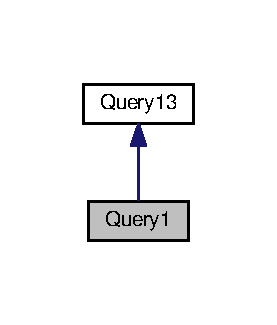
\includegraphics[width=133pt]{classQuery1__inherit__graph}
\end{center}
\end{figure}


Collaboration diagram for Query1\+:\nopagebreak
\begin{figure}[H]
\begin{center}
\leavevmode
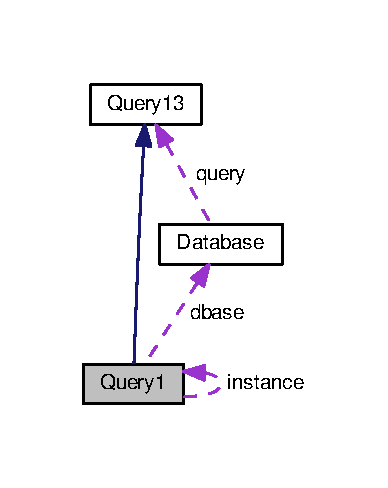
\includegraphics[width=186pt]{classQuery1__coll__graph}
\end{center}
\end{figure}
\subsection*{Public Member Functions}
\begin{DoxyCompactItemize}
\item 
\hyperlink{classQuery1_aca728525a5aaf4f2a993a414eb4495b2}{Query1} (String \+\_\+filename)
\item 
void \hyperlink{classQuery1_a13c86103ce4bda48db0a398a7d7d107c}{find} (int \+\_\+mode, String \+\_\+q, int \+\_\+since, int \+\_\+to, int \+\_\+sort\+Mode)
\item 
void \hyperlink{classQuery1_a5c7f9b2155dfe6bde03c6579fb00b61a}{check} (\hyperlink{classDataRecords}{Data\+Records} d)
\item 
\hyperlink{classDataRecords}{Data\+Records} \hyperlink{classQuery1_a3590292b24792c860c2dedb170683497}{get\+Data} ()
\item 
int \hyperlink{classQuery1_a6c3cfaf81d41e28b40f835d533865182}{get\+Count} ()
\item 
void \hyperlink{classQuery1_a4ac5185895a11f7dd7906a22d8854caf}{print\+Data} ()
\item 
int \hyperlink{classQuery1_a1fe6a57adb424a935bedb8a7ca6cf40f}{get\+Distance} (String s, String t)
\end{DoxyCompactItemize}
\subsection*{Static Public Member Functions}
\begin{DoxyCompactItemize}
\item 
static \hyperlink{classQuery1}{Query1} \hyperlink{classQuery1_a2b63c437c3dbe7c615254a629bdd742f}{get\+Instance} ()
\end{DoxyCompactItemize}
\subsection*{Private Attributes}
\begin{DoxyCompactItemize}
\item 
\hyperlink{classDatabase}{Database} \hyperlink{classQuery1_af7fea4172dbe6f682854a92fed28e583}{dbase}
\item 
String \hyperlink{classQuery1_a747a19c9f4b24c9c47f7c7f13e8932e7}{filename}
\item 
int \hyperlink{classQuery1_a91868e1771a4ea60d950ffd61c56827d}{mode}
\item 
String \hyperlink{classQuery1_acaa7bb7db670b4e6ffce9380b960b9e3}{q}
\item 
Priority\+Queue$<$ \hyperlink{classDataRecords}{Data\+Records} $>$ \hyperlink{classQuery1_a418a5ab9b0660ea8b3c5481beb385bbc}{data\+Rec}
\item 
Priority\+Queue$<$ \hyperlink{classDataRecords}{Data\+Records} $>$ \hyperlink{classQuery1_ace614dbbc820194d2c7092827b9c2491}{data\+Rec2}
\item 
int \hyperlink{classQuery1_a916bfb3d18a8fa0663bfc9728d40961f}{count} =0
\end{DoxyCompactItemize}
\subsection*{Static Private Attributes}
\begin{DoxyCompactItemize}
\item 
static \hyperlink{classQuery1}{Query1} \hyperlink{classQuery1_aca7ee51acbe7e939d39bbd950738fef2}{instance} = new \hyperlink{classQuery1}{Query1}(\char`\"{}dblp.\+xml\char`\"{})
\end{DoxyCompactItemize}


\subsection{Detailed Description}
This class uses \hyperlink{classDatabase}{Database} to extract data as needed for \hyperlink{classQuery1}{Query1}, the class is Singleton 

\subsection{Constructor \& Destructor Documentation}
\index{Query1@{Query1}!Query1@{Query1}}
\index{Query1@{Query1}!Query1@{Query1}}
\subsubsection[{\texorpdfstring{Query1(\+String \+\_\+filename)}{Query1(String _filename)}}]{\setlength{\rightskip}{0pt plus 5cm}Query1.\+Query1 (
\begin{DoxyParamCaption}
\item[{String}]{\+\_\+filename}
\end{DoxyParamCaption}
)\hspace{0.3cm}{\ttfamily [inline]}}\hypertarget{classQuery1_aca728525a5aaf4f2a993a414eb4495b2}{}\label{classQuery1_aca728525a5aaf4f2a993a414eb4495b2}

\begin{DoxyCode}
19                                    \{
20         \hyperlink{classQuery1_a747a19c9f4b24c9c47f7c7f13e8932e7}{filename} = \_filename;
21     \}
\end{DoxyCode}


\subsection{Member Function Documentation}
\index{Query1@{Query1}!check@{check}}
\index{check@{check}!Query1@{Query1}}
\subsubsection[{\texorpdfstring{check(\+Data\+Records d)}{check(DataRecords d)}}]{\setlength{\rightskip}{0pt plus 5cm}void Query1.\+check (
\begin{DoxyParamCaption}
\item[{{\bf Data\+Records}}]{d}
\end{DoxyParamCaption}
)\hspace{0.3cm}{\ttfamily [inline]}}\hypertarget{classQuery1_a5c7f9b2155dfe6bde03c6579fb00b61a}{}\label{classQuery1_a5c7f9b2155dfe6bde03c6579fb00b61a}


Implements \hyperlink{interfaceQuery13_aa8625da54bbd25beb6968df65fe05e57}{Query13}.


\begin{DoxyCode}
44                                     \{
45         \textcolor{keywordtype}{int} t;
46         \textcolor{keywordflow}{if} (\hyperlink{classQuery1_a91868e1771a4ea60d950ffd61c56827d}{mode} == 1 && d.\hyperlink{classDataRecords_a9b0dba84ec8d539395853caff7d4080f}{getAuthor}() != null)\{
47             String[] authors = d.\hyperlink{classDataRecords_a9b0dba84ec8d539395853caff7d4080f}{getAuthor}().split(\textcolor{stringliteral}{","});
48             \textcolor{keywordflow}{for} (String a : authors)\{
49                 \textcolor{keywordflow}{if} (\hyperlink{classAuthorManager}{AuthorManager}.\hyperlink{classAuthorManager_a2442f65701e05d1c2f9f7edb473cb0f3}{resolveAuthor}(a.toLowerCase()) == 
      \hyperlink{classAuthorManager}{AuthorManager}.\hyperlink{classAuthorManager_a2442f65701e05d1c2f9f7edb473cb0f3}{resolveAuthor}(\hyperlink{classQuery1_acaa7bb7db670b4e6ffce9380b960b9e3}{q}) && d.\hyperlink{classDataRecords_a9918de1a257be6b753ef46d66c43989c}{getYear}() >= since && d.
      \hyperlink{classDataRecords_a9918de1a257be6b753ef46d66c43989c}{getYear}() <= to)\{
50                     \hyperlink{classQuery1_a418a5ab9b0660ea8b3c5481beb385bbc}{dataRec}.add(d);
51                     \hyperlink{classQuery1_a916bfb3d18a8fa0663bfc9728d40961f}{count}++;
52                 \}
53             \}
54         \}       
55         \textcolor{keywordflow}{else} \textcolor{keywordflow}{if} (sortMode==0 && \hyperlink{classQuery1_a91868e1771a4ea60d950ffd61c56827d}{mode} == 2 && d.\hyperlink{classDataRecords_a2b6d27b078eb3a16734562f9ded6e1c6}{getTitle}()!=null && (t=this.
      \hyperlink{classQuery1_a1fe6a57adb424a935bedb8a7ca6cf40f}{getDistance}(\hyperlink{classQuery1_acaa7bb7db670b4e6ffce9380b960b9e3}{q}.toLowerCase(), d.\hyperlink{classDataRecords_a2b6d27b078eb3a16734562f9ded6e1c6}{getTitle}()))>0 && d.\hyperlink{classDataRecords_a9918de1a257be6b753ef46d66c43989c}{getYear}() >= since && d.
      \hyperlink{classDataRecords_a9918de1a257be6b753ef46d66c43989c}{getYear}() <= to)\{
56             \hyperlink{classQuery1_a418a5ab9b0660ea8b3c5481beb385bbc}{dataRec}.add(d);
57             \hyperlink{classQuery1_a916bfb3d18a8fa0663bfc9728d40961f}{count}++;
58         \} 
59         \textcolor{keywordflow}{else} \textcolor{keywordflow}{if} (sortMode==1 && \hyperlink{classQuery1_a91868e1771a4ea60d950ffd61c56827d}{mode} == 2 && d.\hyperlink{classDataRecords_a2b6d27b078eb3a16734562f9ded6e1c6}{getTitle}()!=null && (t=this.
      \hyperlink{classQuery1_a1fe6a57adb424a935bedb8a7ca6cf40f}{getDistance}(\hyperlink{classQuery1_acaa7bb7db670b4e6ffce9380b960b9e3}{q}.toLowerCase(), d.\hyperlink{classDataRecords_a2b6d27b078eb3a16734562f9ded6e1c6}{getTitle}()))>0 && d.\hyperlink{classDataRecords_a9918de1a257be6b753ef46d66c43989c}{getYear}() >= since && d.
      \hyperlink{classDataRecords_a9918de1a257be6b753ef46d66c43989c}{getYear}() <= to)\{
60             \textcolor{keywordflow}{if} (t>d.\hyperlink{classDataRecords_a7487a30fa32c0f7e8a05f26b6f23f25a}{getStringMatch}())
61                 d.\hyperlink{classDataRecords_a1e41c4c115595d47b7bbf4016919ff8c}{setStringMatch}(t);
62             \hyperlink{classQuery1_ace614dbbc820194d2c7092827b9c2491}{dataRec2}.add(d);
63             \hyperlink{classQuery1_a916bfb3d18a8fa0663bfc9728d40961f}{count}++;
64         \} 
65     \}
\end{DoxyCode}
\index{Query1@{Query1}!find@{find}}
\index{find@{find}!Query1@{Query1}}
\subsubsection[{\texorpdfstring{find(int \+\_\+mode, String \+\_\+q, int \+\_\+since, int \+\_\+to, int \+\_\+sort\+Mode)}{find(int _mode, String _q, int _since, int _to, int _sortMode)}}]{\setlength{\rightskip}{0pt plus 5cm}void Query1.\+find (
\begin{DoxyParamCaption}
\item[{int}]{\+\_\+mode, }
\item[{String}]{\+\_\+q, }
\item[{int}]{\+\_\+since, }
\item[{int}]{\+\_\+to, }
\item[{int}]{\+\_\+sort\+Mode}
\end{DoxyParamCaption}
)\hspace{0.3cm}{\ttfamily [inline]}}\hypertarget{classQuery1_a13c86103ce4bda48db0a398a7d7d107c}{}\label{classQuery1_a13c86103ce4bda48db0a398a7d7d107c}
This method starts the finding of relevant data 
\begin{DoxyCode}
23                                                                              \{
24         \hyperlink{classQuery1_a418a5ab9b0660ea8b3c5481beb385bbc}{dataRec} = \textcolor{keyword}{new} PriorityQueue<DataRecords>();
25         \hyperlink{classQuery1_ace614dbbc820194d2c7092827b9c2491}{dataRec2} = \textcolor{keyword}{new} PriorityQueue<DataRecords>(\textcolor{keyword}{new} Comparator<DataRecords>() \{
26                 \textcolor{keyword}{public} \textcolor{keywordtype}{int} compare(\hyperlink{classDataRecords}{DataRecords} d1, \hyperlink{classDataRecords}{DataRecords} d2) \{
27                     \textcolor{keywordflow}{if}(d1.\hyperlink{classDataRecords_a7487a30fa32c0f7e8a05f26b6f23f25a}{getStringMatch}()<d2.\hyperlink{classDataRecords_a7487a30fa32c0f7e8a05f26b6f23f25a}{getStringMatch}())\{
28                         \textcolor{keywordflow}{return} 1;
29                     \}            
30                     \textcolor{keywordflow}{else} \textcolor{keywordflow}{if}(d1.\hyperlink{classDataRecords_a7487a30fa32c0f7e8a05f26b6f23f25a}{getStringMatch}()==d2.\hyperlink{classDataRecords_a7487a30fa32c0f7e8a05f26b6f23f25a}{getStringMatch}())\{
31                         \textcolor{keywordflow}{return} 0;
32                     \} 
33                     \textcolor{keywordflow}{return} -1;                                               
34                 \}
35             \});
36         \hyperlink{classQuery1_a91868e1771a4ea60d950ffd61c56827d}{mode} = \_mode;
37         since = \_since;
38         to = \_to;
39         sortMode=\_sortMode;
40         \hyperlink{classQuery1_acaa7bb7db670b4e6ffce9380b960b9e3}{q} = \_q.toLowerCase();
41         \hyperlink{classQuery1_a916bfb3d18a8fa0663bfc9728d40961f}{count}=0;
42         \hyperlink{classQuery1_af7fea4172dbe6f682854a92fed28e583}{dbase} = \textcolor{keyword}{new} \hyperlink{classDatabase}{Database}(\hyperlink{classQuery1_a747a19c9f4b24c9c47f7c7f13e8932e7}{filename}, \textcolor{keyword}{this});
43     \}
\end{DoxyCode}
\index{Query1@{Query1}!get\+Count@{get\+Count}}
\index{get\+Count@{get\+Count}!Query1@{Query1}}
\subsubsection[{\texorpdfstring{get\+Count()}{getCount()}}]{\setlength{\rightskip}{0pt plus 5cm}int Query1.\+get\+Count (
\begin{DoxyParamCaption}
{}
\end{DoxyParamCaption}
)\hspace{0.3cm}{\ttfamily [inline]}}\hypertarget{classQuery1_a6c3cfaf81d41e28b40f835d533865182}{}\label{classQuery1_a6c3cfaf81d41e28b40f835d533865182}
Gets the total number of results 
\begin{DoxyCode}
76                          \{
77         \textcolor{keywordflow}{return} \hyperlink{classQuery1_a916bfb3d18a8fa0663bfc9728d40961f}{count};
78     \}
\end{DoxyCode}
\index{Query1@{Query1}!get\+Data@{get\+Data}}
\index{get\+Data@{get\+Data}!Query1@{Query1}}
\subsubsection[{\texorpdfstring{get\+Data()}{getData()}}]{\setlength{\rightskip}{0pt plus 5cm}{\bf Data\+Records} Query1.\+get\+Data (
\begin{DoxyParamCaption}
{}
\end{DoxyParamCaption}
)\hspace{0.3cm}{\ttfamily [inline]}}\hypertarget{classQuery1_a3590292b24792c860c2dedb170683497}{}\label{classQuery1_a3590292b24792c860c2dedb170683497}
This method gives back data one element at a time returning null when finished 
\begin{DoxyCode}
67                                 \{
68         \textcolor{keywordflow}{if}(\hyperlink{classQuery1_a91868e1771a4ea60d950ffd61c56827d}{mode}== 1 && (sortMode==0 || sortMode ==1))
69             \textcolor{keywordflow}{return} \hyperlink{classQuery1_a418a5ab9b0660ea8b3c5481beb385bbc}{dataRec}.poll();
70         \textcolor{keywordflow}{else} \textcolor{keywordflow}{if}(\hyperlink{classQuery1_a91868e1771a4ea60d950ffd61c56827d}{mode}==2 && (sortMode==0))
71             \textcolor{keywordflow}{return} \hyperlink{classQuery1_a418a5ab9b0660ea8b3c5481beb385bbc}{dataRec}.poll();
72         \textcolor{keywordflow}{else}
73             \textcolor{keywordflow}{return} \hyperlink{classQuery1_ace614dbbc820194d2c7092827b9c2491}{dataRec2}.poll();     
74     \}
\end{DoxyCode}
\index{Query1@{Query1}!get\+Distance@{get\+Distance}}
\index{get\+Distance@{get\+Distance}!Query1@{Query1}}
\subsubsection[{\texorpdfstring{get\+Distance(\+String s, String t)}{getDistance(String s, String t)}}]{\setlength{\rightskip}{0pt plus 5cm}int Query1.\+get\+Distance (
\begin{DoxyParamCaption}
\item[{String}]{s, }
\item[{String}]{t}
\end{DoxyParamCaption}
)\hspace{0.3cm}{\ttfamily [inline]}}\hypertarget{classQuery1_a1fe6a57adb424a935bedb8a7ca6cf40f}{}\label{classQuery1_a1fe6a57adb424a935bedb8a7ca6cf40f}

\begin{DoxyCode}
91                                               \{
92         String[] arr = s.split(\textcolor{stringliteral}{" "});  
93         String[] arr2 = t.split(\textcolor{stringliteral}{" "});
94         \textcolor{keywordtype}{int} \hyperlink{classQuery1_a916bfb3d18a8fa0663bfc9728d40961f}{count}=0;
95         \textcolor{keywordflow}{for}(String a:arr)\{
96             \textcolor{keywordflow}{for}(String b:arr2)\{
97                 \textcolor{keywordflow}{if}(a.equalsIgnoreCase(b) && b.length()>=4)\{
98                     count++;
99                     \textcolor{keywordflow}{break};
100                 \}
101             \}
102         \}  
103         \textcolor{keywordflow}{return} \hyperlink{classQuery1_a916bfb3d18a8fa0663bfc9728d40961f}{count};
104     \}
\end{DoxyCode}
\index{Query1@{Query1}!get\+Instance@{get\+Instance}}
\index{get\+Instance@{get\+Instance}!Query1@{Query1}}
\subsubsection[{\texorpdfstring{get\+Instance()}{getInstance()}}]{\setlength{\rightskip}{0pt plus 5cm}static {\bf Query1} Query1.\+get\+Instance (
\begin{DoxyParamCaption}
{}
\end{DoxyParamCaption}
)\hspace{0.3cm}{\ttfamily [inline]}, {\ttfamily [static]}}\hypertarget{classQuery1_a2b63c437c3dbe7c615254a629bdd742f}{}\label{classQuery1_a2b63c437c3dbe7c615254a629bdd742f}

\begin{DoxyCode}
105                                       \{
106         \textcolor{keywordflow}{return} \hyperlink{classQuery1_aca7ee51acbe7e939d39bbd950738fef2}{instance};
107     \}
\end{DoxyCode}
\index{Query1@{Query1}!print\+Data@{print\+Data}}
\index{print\+Data@{print\+Data}!Query1@{Query1}}
\subsubsection[{\texorpdfstring{print\+Data()}{printData()}}]{\setlength{\rightskip}{0pt plus 5cm}void Query1.\+print\+Data (
\begin{DoxyParamCaption}
{}
\end{DoxyParamCaption}
)\hspace{0.3cm}{\ttfamily [inline]}}\hypertarget{classQuery1_a4ac5185895a11f7dd7906a22d8854caf}{}\label{classQuery1_a4ac5185895a11f7dd7906a22d8854caf}


Implements \hyperlink{interfaceQuery13_a7b04f8c829e445286d760995b0205ded}{Query13}.


\begin{DoxyCode}
79                            \{
80         \hyperlink{classDataRecords}{DataRecords} d;
81         System.out.println(\textcolor{stringliteral}{"size- "}+\hyperlink{classQuery1_a418a5ab9b0660ea8b3c5481beb385bbc}{dataRec}.size());
82         \textcolor{keywordflow}{while} ((d = \hyperlink{classQuery1_a418a5ab9b0660ea8b3c5481beb385bbc}{dataRec}.poll())!=null)\{
83             System.out.println(d.\hyperlink{classDataRecords_a2b6d27b078eb3a16734562f9ded6e1c6}{getTitle}());
84             String[] authors = d.\hyperlink{classDataRecords_a9b0dba84ec8d539395853caff7d4080f}{getAuthor}().split(\textcolor{stringliteral}{","});
85                 \textcolor{keywordflow}{for} (String a : authors)\{
86                     System.out.print(a+\textcolor{stringliteral}{" "});
87                 \}
88                 System.out.println(\textcolor{stringliteral}{" "});
89         \}
90     \}
\end{DoxyCode}


\subsection{Member Data Documentation}
\index{Query1@{Query1}!count@{count}}
\index{count@{count}!Query1@{Query1}}
\subsubsection[{\texorpdfstring{count}{count}}]{\setlength{\rightskip}{0pt plus 5cm}int Query1.\+count =0\hspace{0.3cm}{\ttfamily [private]}}\hypertarget{classQuery1_a916bfb3d18a8fa0663bfc9728d40961f}{}\label{classQuery1_a916bfb3d18a8fa0663bfc9728d40961f}
\index{Query1@{Query1}!data\+Rec@{data\+Rec}}
\index{data\+Rec@{data\+Rec}!Query1@{Query1}}
\subsubsection[{\texorpdfstring{data\+Rec}{dataRec}}]{\setlength{\rightskip}{0pt plus 5cm}Priority\+Queue$<${\bf Data\+Records}$>$ Query1.\+data\+Rec\hspace{0.3cm}{\ttfamily [private]}}\hypertarget{classQuery1_a418a5ab9b0660ea8b3c5481beb385bbc}{}\label{classQuery1_a418a5ab9b0660ea8b3c5481beb385bbc}
\index{Query1@{Query1}!data\+Rec2@{data\+Rec2}}
\index{data\+Rec2@{data\+Rec2}!Query1@{Query1}}
\subsubsection[{\texorpdfstring{data\+Rec2}{dataRec2}}]{\setlength{\rightskip}{0pt plus 5cm}Priority\+Queue$<${\bf Data\+Records}$>$ Query1.\+data\+Rec2\hspace{0.3cm}{\ttfamily [private]}}\hypertarget{classQuery1_ace614dbbc820194d2c7092827b9c2491}{}\label{classQuery1_ace614dbbc820194d2c7092827b9c2491}
\index{Query1@{Query1}!dbase@{dbase}}
\index{dbase@{dbase}!Query1@{Query1}}
\subsubsection[{\texorpdfstring{dbase}{dbase}}]{\setlength{\rightskip}{0pt plus 5cm}{\bf Database} Query1.\+dbase\hspace{0.3cm}{\ttfamily [private]}}\hypertarget{classQuery1_af7fea4172dbe6f682854a92fed28e583}{}\label{classQuery1_af7fea4172dbe6f682854a92fed28e583}
\index{Query1@{Query1}!filename@{filename}}
\index{filename@{filename}!Query1@{Query1}}
\subsubsection[{\texorpdfstring{filename}{filename}}]{\setlength{\rightskip}{0pt plus 5cm}String Query1.\+filename\hspace{0.3cm}{\ttfamily [private]}}\hypertarget{classQuery1_a747a19c9f4b24c9c47f7c7f13e8932e7}{}\label{classQuery1_a747a19c9f4b24c9c47f7c7f13e8932e7}
\index{Query1@{Query1}!instance@{instance}}
\index{instance@{instance}!Query1@{Query1}}
\subsubsection[{\texorpdfstring{instance}{instance}}]{\setlength{\rightskip}{0pt plus 5cm}{\bf Query1} Query1.\+instance = new {\bf Query1}(\char`\"{}dblp.\+xml\char`\"{})\hspace{0.3cm}{\ttfamily [static]}, {\ttfamily [private]}}\hypertarget{classQuery1_aca7ee51acbe7e939d39bbd950738fef2}{}\label{classQuery1_aca7ee51acbe7e939d39bbd950738fef2}
\index{Query1@{Query1}!mode@{mode}}
\index{mode@{mode}!Query1@{Query1}}
\subsubsection[{\texorpdfstring{mode}{mode}}]{\setlength{\rightskip}{0pt plus 5cm}int Query1.\+mode\hspace{0.3cm}{\ttfamily [private]}}\hypertarget{classQuery1_a91868e1771a4ea60d950ffd61c56827d}{}\label{classQuery1_a91868e1771a4ea60d950ffd61c56827d}
\index{Query1@{Query1}!q@{q}}
\index{q@{q}!Query1@{Query1}}
\subsubsection[{\texorpdfstring{q}{q}}]{\setlength{\rightskip}{0pt plus 5cm}String Query1.\+q\hspace{0.3cm}{\ttfamily [private]}}\hypertarget{classQuery1_acaa7bb7db670b4e6ffce9380b960b9e3}{}\label{classQuery1_acaa7bb7db670b4e6ffce9380b960b9e3}


The documentation for this class was generated from the following file\+:\begin{DoxyCompactItemize}
\item 
\hyperlink{Query1_8java}{Query1.\+java}\end{DoxyCompactItemize}

\hypertarget{interfaceQuery13}{}\section{Query13 Interface Reference}
\label{interfaceQuery13}\index{Query13@{Query13}}


Inheritance diagram for Query13\+:\nopagebreak
\begin{figure}[H]
\begin{center}
\leavevmode
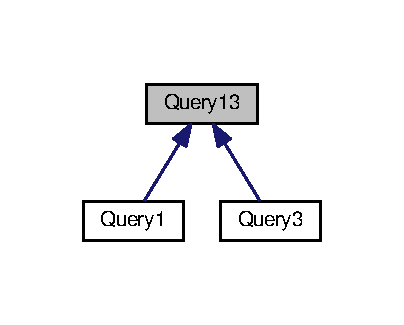
\includegraphics[width=194pt]{interfaceQuery13__inherit__graph}
\end{center}
\end{figure}
\subsection*{Public Member Functions}
\begin{DoxyCompactItemize}
\item 
void \hyperlink{interfaceQuery13_aa8625da54bbd25beb6968df65fe05e57}{check} (\hyperlink{classDataRecords}{Data\+Records} d)
\item 
void \hyperlink{interfaceQuery13_a7b04f8c829e445286d760995b0205ded}{print\+Data} ()
\end{DoxyCompactItemize}


\subsection{Member Function Documentation}
\index{Query13@{Query13}!check@{check}}
\index{check@{check}!Query13@{Query13}}
\subsubsection[{\texorpdfstring{check(\+Data\+Records d)}{check(DataRecords d)}}]{\setlength{\rightskip}{0pt plus 5cm}void Query13.\+check (
\begin{DoxyParamCaption}
\item[{{\bf Data\+Records}}]{d}
\end{DoxyParamCaption}
)}\hypertarget{interfaceQuery13_aa8625da54bbd25beb6968df65fe05e57}{}\label{interfaceQuery13_aa8625da54bbd25beb6968df65fe05e57}


Implemented in \hyperlink{classQuery1_a5c7f9b2155dfe6bde03c6579fb00b61a}{Query1}, and \hyperlink{classQuery3_aa427e3890ba5a50c0fe65f8ec8c0b451}{Query3}.

\index{Query13@{Query13}!print\+Data@{print\+Data}}
\index{print\+Data@{print\+Data}!Query13@{Query13}}
\subsubsection[{\texorpdfstring{print\+Data()}{printData()}}]{\setlength{\rightskip}{0pt plus 5cm}void Query13.\+print\+Data (
\begin{DoxyParamCaption}
{}
\end{DoxyParamCaption}
)}\hypertarget{interfaceQuery13_a7b04f8c829e445286d760995b0205ded}{}\label{interfaceQuery13_a7b04f8c829e445286d760995b0205ded}


Implemented in \hyperlink{classQuery1_a4ac5185895a11f7dd7906a22d8854caf}{Query1}, and \hyperlink{classQuery3_a6cde68ceca0e88d2af13e31a5de0e9a4}{Query3}.



The documentation for this interface was generated from the following file\+:\begin{DoxyCompactItemize}
\item 
\hyperlink{Query13_8java}{Query13.\+java}\end{DoxyCompactItemize}

\hypertarget{classQuery2}{}\section{Query2 Class Reference}
\label{classQuery2}\index{Query2@{Query2}}


Collaboration diagram for Query2\+:\nopagebreak
\begin{figure}[H]
\begin{center}
\leavevmode
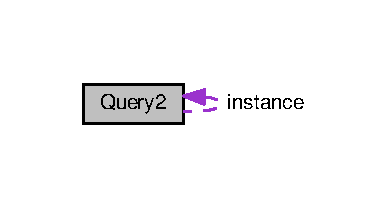
\includegraphics[width=186pt]{classQuery2__coll__graph}
\end{center}
\end{figure}
\subsection*{Public Member Functions}
\begin{DoxyCompactItemize}
\item 
void \hyperlink{classQuery2_ab5f9fd59b15dcdef599faec26ae49424}{find} (int k)
\item 
\hyperlink{classAuthor}{Author} \hyperlink{classQuery2_a70190cc13fb74f6bf00ce1347a8b8946}{get\+Data} ()
\item 
void \hyperlink{classQuery2_ae1f51e2c333e090fcd07a573a2ba7b10}{print\+Data} ()
\item 
int \hyperlink{classQuery2_afc9171c552d575feafb5e5f4b3a6cc19}{get\+Count} ()
\end{DoxyCompactItemize}
\subsection*{Static Public Member Functions}
\begin{DoxyCompactItemize}
\item 
static \hyperlink{classQuery2}{Query2} \hyperlink{classQuery2_a0a1270d32e0b8ac467ad09f546e0c3ee}{get\+Instance} ()
\end{DoxyCompactItemize}
\subsection*{Private Member Functions}
\begin{DoxyCompactItemize}
\item 
\hyperlink{classQuery2_ad2ab065a532d46e6a40c16fff5041a52}{Query2} (String \+\_\+filename)
\end{DoxyCompactItemize}
\subsection*{Private Attributes}
\begin{DoxyCompactItemize}
\item 
Array\+List$<$ \hyperlink{classAuthor}{Author} $>$ \hyperlink{classQuery2_a0e6787ef46755e839db06e99a090e311}{result}
\item 
String \hyperlink{classQuery2_a2e312018f6ecd6d6b58e5ada0338ef6c}{filename}
\end{DoxyCompactItemize}
\subsection*{Static Private Attributes}
\begin{DoxyCompactItemize}
\item 
static \hyperlink{classQuery2}{Query2} \hyperlink{classQuery2_ad0d6f793ef89bb9a3a82358a30cd086d}{instance} = new \hyperlink{classQuery2}{Query2}(\char`\"{}dblp.\+xml\char`\"{})
\end{DoxyCompactItemize}


\subsection{Detailed Description}
This class uses \hyperlink{classDatabase}{Database} to extract data as needed for \hyperlink{classQuery2}{Query2}, the class is Singleton 

\subsection{Constructor \& Destructor Documentation}
\index{Query2@{Query2}!Query2@{Query2}}
\index{Query2@{Query2}!Query2@{Query2}}
\subsubsection[{\texorpdfstring{Query2(\+String \+\_\+filename)}{Query2(String _filename)}}]{\setlength{\rightskip}{0pt plus 5cm}Query2.\+Query2 (
\begin{DoxyParamCaption}
\item[{String}]{\+\_\+filename}
\end{DoxyParamCaption}
)\hspace{0.3cm}{\ttfamily [inline]}, {\ttfamily [private]}}\hypertarget{classQuery2_ad2ab065a532d46e6a40c16fff5041a52}{}\label{classQuery2_ad2ab065a532d46e6a40c16fff5041a52}

\begin{DoxyCode}
14                                     \{
15         \hyperlink{classQuery2_a2e312018f6ecd6d6b58e5ada0338ef6c}{filename} = \_filename;
16     \}
\end{DoxyCode}


\subsection{Member Function Documentation}
\index{Query2@{Query2}!find@{find}}
\index{find@{find}!Query2@{Query2}}
\subsubsection[{\texorpdfstring{find(int k)}{find(int k)}}]{\setlength{\rightskip}{0pt plus 5cm}void Query2.\+find (
\begin{DoxyParamCaption}
\item[{int}]{k}
\end{DoxyParamCaption}
)\hspace{0.3cm}{\ttfamily [inline]}}\hypertarget{classQuery2_ab5f9fd59b15dcdef599faec26ae49424}{}\label{classQuery2_ab5f9fd59b15dcdef599faec26ae49424}
This method starts the finding of relevant data 
\begin{DoxyCode}
18                            \{
19         \hyperlink{classQuery2_a0e6787ef46755e839db06e99a090e311}{result} = \hyperlink{classAuthorManager}{AuthorManager}.\hyperlink{classAuthorManager_a7aa5758d30203dc5f31f19154a15ec82}{getGreaterK}(k);
20     \}
\end{DoxyCode}
\index{Query2@{Query2}!get\+Count@{get\+Count}}
\index{get\+Count@{get\+Count}!Query2@{Query2}}
\subsubsection[{\texorpdfstring{get\+Count()}{getCount()}}]{\setlength{\rightskip}{0pt plus 5cm}int Query2.\+get\+Count (
\begin{DoxyParamCaption}
{}
\end{DoxyParamCaption}
)\hspace{0.3cm}{\ttfamily [inline]}}\hypertarget{classQuery2_afc9171c552d575feafb5e5f4b3a6cc19}{}\label{classQuery2_afc9171c552d575feafb5e5f4b3a6cc19}
Gets the total number of results 
\begin{DoxyCode}
37                          \{
38         \textcolor{keywordflow}{return} \hyperlink{classQuery2_a0e6787ef46755e839db06e99a090e311}{result}.size();
39     \}
\end{DoxyCode}
\index{Query2@{Query2}!get\+Data@{get\+Data}}
\index{get\+Data@{get\+Data}!Query2@{Query2}}
\subsubsection[{\texorpdfstring{get\+Data()}{getData()}}]{\setlength{\rightskip}{0pt plus 5cm}{\bf Author} Query2.\+get\+Data (
\begin{DoxyParamCaption}
{}
\end{DoxyParamCaption}
)\hspace{0.3cm}{\ttfamily [inline]}}\hypertarget{classQuery2_a70190cc13fb74f6bf00ce1347a8b8946}{}\label{classQuery2_a70190cc13fb74f6bf00ce1347a8b8946}
This method gives back data one element at a time returning null when finished 
\begin{DoxyCode}
22                            \{
23         \textcolor{keywordflow}{if} (\hyperlink{classQuery2_a0e6787ef46755e839db06e99a090e311}{result}.size() == 0)
24             \textcolor{keywordflow}{return} null;
25         \textcolor{keywordflow}{else}\{
26             \hyperlink{classAuthor}{Author} a = \hyperlink{classQuery2_a0e6787ef46755e839db06e99a090e311}{result}.get(0);
27             \hyperlink{classQuery2_a0e6787ef46755e839db06e99a090e311}{result}.remove(0);
28             \textcolor{keywordflow}{return} a;
29         \}
30     \}
\end{DoxyCode}
\index{Query2@{Query2}!get\+Instance@{get\+Instance}}
\index{get\+Instance@{get\+Instance}!Query2@{Query2}}
\subsubsection[{\texorpdfstring{get\+Instance()}{getInstance()}}]{\setlength{\rightskip}{0pt plus 5cm}static {\bf Query2} Query2.\+get\+Instance (
\begin{DoxyParamCaption}
{}
\end{DoxyParamCaption}
)\hspace{0.3cm}{\ttfamily [inline]}, {\ttfamily [static]}}\hypertarget{classQuery2_a0a1270d32e0b8ac467ad09f546e0c3ee}{}\label{classQuery2_a0a1270d32e0b8ac467ad09f546e0c3ee}

\begin{DoxyCode}
40                                       \{
41         \textcolor{keywordflow}{return} \hyperlink{classQuery2_ad0d6f793ef89bb9a3a82358a30cd086d}{instance};
42     \}
\end{DoxyCode}
\index{Query2@{Query2}!print\+Data@{print\+Data}}
\index{print\+Data@{print\+Data}!Query2@{Query2}}
\subsubsection[{\texorpdfstring{print\+Data()}{printData()}}]{\setlength{\rightskip}{0pt plus 5cm}void Query2.\+print\+Data (
\begin{DoxyParamCaption}
{}
\end{DoxyParamCaption}
)\hspace{0.3cm}{\ttfamily [inline]}}\hypertarget{classQuery2_ae1f51e2c333e090fcd07a573a2ba7b10}{}\label{classQuery2_ae1f51e2c333e090fcd07a573a2ba7b10}

\begin{DoxyCode}
31                            \{
32         \textcolor{keywordflow}{for} (\hyperlink{classAuthor}{Author} a : \hyperlink{classQuery2_a0e6787ef46755e839db06e99a090e311}{result})\{
33             System.out.println(a.getName() + \textcolor{stringliteral}{" "} + a.getCount());
34         \}
35     \}
\end{DoxyCode}


\subsection{Member Data Documentation}
\index{Query2@{Query2}!filename@{filename}}
\index{filename@{filename}!Query2@{Query2}}
\subsubsection[{\texorpdfstring{filename}{filename}}]{\setlength{\rightskip}{0pt plus 5cm}String Query2.\+filename\hspace{0.3cm}{\ttfamily [private]}}\hypertarget{classQuery2_a2e312018f6ecd6d6b58e5ada0338ef6c}{}\label{classQuery2_a2e312018f6ecd6d6b58e5ada0338ef6c}
\index{Query2@{Query2}!instance@{instance}}
\index{instance@{instance}!Query2@{Query2}}
\subsubsection[{\texorpdfstring{instance}{instance}}]{\setlength{\rightskip}{0pt plus 5cm}{\bf Query2} Query2.\+instance = new {\bf Query2}(\char`\"{}dblp.\+xml\char`\"{})\hspace{0.3cm}{\ttfamily [static]}, {\ttfamily [private]}}\hypertarget{classQuery2_ad0d6f793ef89bb9a3a82358a30cd086d}{}\label{classQuery2_ad0d6f793ef89bb9a3a82358a30cd086d}
\index{Query2@{Query2}!result@{result}}
\index{result@{result}!Query2@{Query2}}
\subsubsection[{\texorpdfstring{result}{result}}]{\setlength{\rightskip}{0pt plus 5cm}Array\+List$<${\bf Author}$>$ Query2.\+result\hspace{0.3cm}{\ttfamily [private]}}\hypertarget{classQuery2_a0e6787ef46755e839db06e99a090e311}{}\label{classQuery2_a0e6787ef46755e839db06e99a090e311}


The documentation for this class was generated from the following file\+:\begin{DoxyCompactItemize}
\item 
\hyperlink{Query2_8java}{Query2.\+java}\end{DoxyCompactItemize}

\hypertarget{classQuery3}{}\section{Query3 Class Reference}
\label{classQuery3}\index{Query3@{Query3}}


Inheritance diagram for Query3\+:\nopagebreak
\begin{figure}[H]
\begin{center}
\leavevmode
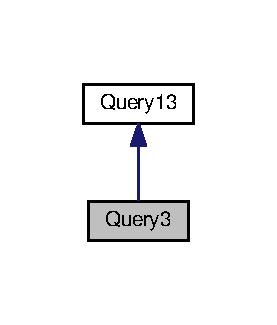
\includegraphics[width=133pt]{classQuery3__inherit__graph}
\end{center}
\end{figure}


Collaboration diagram for Query3\+:\nopagebreak
\begin{figure}[H]
\begin{center}
\leavevmode
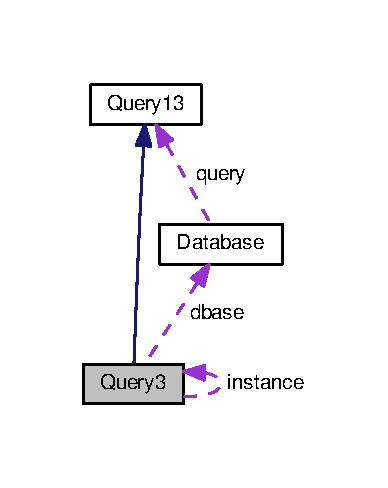
\includegraphics[width=186pt]{classQuery3__coll__graph}
\end{center}
\end{figure}
\subsection*{Public Member Functions}
\begin{DoxyCompactItemize}
\item 
void \hyperlink{classQuery3_a90891105629ffe510b97ef9457ee999d}{find} (int \+\_\+year, String \+\_\+auth)
\item 
void \hyperlink{classQuery3_aa427e3890ba5a50c0fe65f8ec8c0b451}{check} (\hyperlink{classDataRecords}{Data\+Records} d)
\item 
void \hyperlink{classQuery3_a6cde68ceca0e88d2af13e31a5de0e9a4}{print\+Data} ()
\item 
double \hyperlink{classQuery3_a165950141428545cd3b1503e2e90b19f}{get\+Data} ()
\item 
int \hyperlink{classQuery3_aaf500171ac702620b4a7cdfdf99511e1}{get\+Degree} ()
\end{DoxyCompactItemize}
\subsection*{Static Public Member Functions}
\begin{DoxyCompactItemize}
\item 
static \hyperlink{classQuery3}{Query3} \hyperlink{classQuery3_a4be96065aec730ecae94b6cd4f086bd1}{get\+Instance} ()
\end{DoxyCompactItemize}
\subsection*{Private Member Functions}
\begin{DoxyCompactItemize}
\item 
\hyperlink{classQuery3_a4fbeb44bc0d6cf64b69c3786079ff607}{Query3} (String \+\_\+filename)
\item 
void \hyperlink{classQuery3_af36aaf92bc68455320f314f748107ba5}{init\+Arrays} ()
\item 
int \hyperlink{classQuery3_a3e717858e45a5e523e6f6822b8ee9c55}{start\+Index} ()
\item 
double \hyperlink{classQuery3_a7cd505a50c7acdad72f8d84e0783d40f}{mean} (int\mbox{[}$\,$\mbox{]} arr)
\item 
long \hyperlink{classQuery3_aed079f7c366024a82d93de739bf748a8}{calc\+Sum} (int\mbox{[}$\,$\mbox{]} a, int i)
\item 
long \hyperlink{classQuery3_a400754740a1332b01276e1219fb23558}{calc\+Mul\+Sum} (int\mbox{[}$\,$\mbox{]} a, int\mbox{[}$\,$\mbox{]} b, int i)
\item 
double \hyperlink{classQuery3_ab20e5f00158bfc416143b645d4ea5f0f}{find\+Slope} ()
\item 
double \hyperlink{classQuery3_ae0e1667d9216468b12b863d0e6b89462}{y\+Intercept} (double x\+Mean, double y\+Mean, double slope)
\item 
double \hyperlink{classQuery3_a9f213eab98fc93aa00e6432d62680982}{linear\+Regression} (int x\+Given)
\end{DoxyCompactItemize}
\subsection*{Private Attributes}
\begin{DoxyCompactItemize}
\item 
\hyperlink{classDatabase}{Database} \hyperlink{classQuery3_acf21ca7cef4efec2a30d041d8b0770f1}{dbase}
\item 
int \hyperlink{classQuery3_a0bae9f7c878eeda85345866f6983caae}{year}
\item 
String \hyperlink{classQuery3_a53f8993bc386e315c22cace0c0405336}{filename}
\item 
String \hyperlink{classQuery3_a2db45c9e219ad331a52169d8f6bacae5}{auth}
\item 
Array\+List$<$ \hyperlink{classDataRecords}{Data\+Records} $>$ \hyperlink{classQuery3_af5c1e99f9d5402273b0a993aa965a6d2}{data\+Rec}
\item 
double\mbox{[}$\,$\mbox{]} \hyperlink{classQuery3_a8357a655699bb076c9174af9c95f00b1}{year\+Reg\+Temp} =null
\item 
double\mbox{[}$\,$\mbox{]} \hyperlink{classQuery3_aa4820280feefd8ebe9c04b42b73c8f52}{pub\+Count\+Temp} =null
\item 
int\mbox{[}$\,$\mbox{]} \hyperlink{classQuery3_ada9c7e6f4d53607da9450738b76dbc7d}{year\+Reg} =null
\item 
int\mbox{[}$\,$\mbox{]} \hyperlink{classQuery3_af016450dd2c9582f3ef5b2979969d201}{pub\+Count} =null
\end{DoxyCompactItemize}
\subsection*{Static Private Attributes}
\begin{DoxyCompactItemize}
\item 
static \hyperlink{classQuery3}{Query3} \hyperlink{classQuery3_a21e9b649c7b92dcd18831c6a1471454a}{instance} = new \hyperlink{classQuery3}{Query3}(\char`\"{}dblp.\+xml\char`\"{})
\end{DoxyCompactItemize}


\subsection{Detailed Description}
This class uses \hyperlink{classDatabase}{Database} to extract data as needed for \hyperlink{classQuery3}{Query3}, the class is Singleton 

\subsection{Constructor \& Destructor Documentation}
\index{Query3@{Query3}!Query3@{Query3}}
\index{Query3@{Query3}!Query3@{Query3}}
\subsubsection[{\texorpdfstring{Query3(\+String \+\_\+filename)}{Query3(String _filename)}}]{\setlength{\rightskip}{0pt plus 5cm}Query3.\+Query3 (
\begin{DoxyParamCaption}
\item[{String}]{\+\_\+filename}
\end{DoxyParamCaption}
)\hspace{0.3cm}{\ttfamily [inline]}, {\ttfamily [private]}}\hypertarget{classQuery3_a4fbeb44bc0d6cf64b69c3786079ff607}{}\label{classQuery3_a4fbeb44bc0d6cf64b69c3786079ff607}

\begin{DoxyCode}
21                                     \{
22         \hyperlink{classQuery3_a53f8993bc386e315c22cace0c0405336}{filename} = \_filename;
23     \}
\end{DoxyCode}


\subsection{Member Function Documentation}
\index{Query3@{Query3}!calc\+Mul\+Sum@{calc\+Mul\+Sum}}
\index{calc\+Mul\+Sum@{calc\+Mul\+Sum}!Query3@{Query3}}
\subsubsection[{\texorpdfstring{calc\+Mul\+Sum(int[] a, int[] b, int i)}{calcMulSum(int[] a, int[] b, int i)}}]{\setlength{\rightskip}{0pt plus 5cm}long Query3.\+calc\+Mul\+Sum (
\begin{DoxyParamCaption}
\item[{int\mbox{[}$\,$\mbox{]}}]{a, }
\item[{int\mbox{[}$\,$\mbox{]}}]{b, }
\item[{int}]{i}
\end{DoxyParamCaption}
)\hspace{0.3cm}{\ttfamily [inline]}, {\ttfamily [private]}}\hypertarget{classQuery3_a400754740a1332b01276e1219fb23558}{}\label{classQuery3_a400754740a1332b01276e1219fb23558}

\begin{DoxyCode}
135     \{
136         \textcolor{keywordtype}{long} mulSum=0;
137         \textcolor{keywordflow}{for}(\textcolor{keywordtype}{int} j=i;j<a.length;j++)
138         \{
139             mulSum+=a[i]*b[i];
140         \}
141         \textcolor{keywordflow}{return} mulSum;
142     \}
\end{DoxyCode}
\index{Query3@{Query3}!calc\+Sum@{calc\+Sum}}
\index{calc\+Sum@{calc\+Sum}!Query3@{Query3}}
\subsubsection[{\texorpdfstring{calc\+Sum(int[] a, int i)}{calcSum(int[] a, int i)}}]{\setlength{\rightskip}{0pt plus 5cm}long Query3.\+calc\+Sum (
\begin{DoxyParamCaption}
\item[{int\mbox{[}$\,$\mbox{]}}]{a, }
\item[{int}]{i}
\end{DoxyParamCaption}
)\hspace{0.3cm}{\ttfamily [inline]}, {\ttfamily [private]}}\hypertarget{classQuery3_aed079f7c366024a82d93de739bf748a8}{}\label{classQuery3_aed079f7c366024a82d93de739bf748a8}

\begin{DoxyCode}
126     \{
127         \textcolor{keywordtype}{long} sum=0;
128         \textcolor{keywordflow}{for}(\textcolor{keywordtype}{int} j=i;j<a.length;j++)
129         \{
130             sum+=a[j];
131         \}
132         \textcolor{keywordflow}{return} sum;
133     \}
\end{DoxyCode}
\index{Query3@{Query3}!check@{check}}
\index{check@{check}!Query3@{Query3}}
\subsubsection[{\texorpdfstring{check(\+Data\+Records d)}{check(DataRecords d)}}]{\setlength{\rightskip}{0pt plus 5cm}void Query3.\+check (
\begin{DoxyParamCaption}
\item[{{\bf Data\+Records}}]{d}
\end{DoxyParamCaption}
)\hspace{0.3cm}{\ttfamily [inline]}}\hypertarget{classQuery3_aa427e3890ba5a50c0fe65f8ec8c0b451}{}\label{classQuery3_aa427e3890ba5a50c0fe65f8ec8c0b451}


Implements \hyperlink{interfaceQuery13_aa8625da54bbd25beb6968df65fe05e57}{Query13}.


\begin{DoxyCode}
39                                     \{
40         \textcolor{keywordflow}{if}(d.\hyperlink{classDataRecords_a9b0dba84ec8d539395853caff7d4080f}{getAuthor}() != null)
41         \{   
42             String[] authors = d.\hyperlink{classDataRecords_a9b0dba84ec8d539395853caff7d4080f}{getAuthor}().split(\textcolor{stringliteral}{","});
43                     \textcolor{keywordflow}{for} (String a : authors)\{
44                         \textcolor{keywordflow}{if} (\hyperlink{classAuthorManager}{AuthorManager}.\hyperlink{classAuthorManager_a2442f65701e05d1c2f9f7edb473cb0f3}{resolveAuthor}(a.toLowerCase()) == 
      \hyperlink{classAuthorManager}{AuthorManager}.\hyperlink{classAuthorManager_a2442f65701e05d1c2f9f7edb473cb0f3}{resolveAuthor}(\hyperlink{classQuery3_a2db45c9e219ad331a52169d8f6bacae5}{auth}) && d.\hyperlink{classDataRecords_a9918de1a257be6b753ef46d66c43989c}{getYear}() !=0 && d.
      \hyperlink{classDataRecords_a9918de1a257be6b753ef46d66c43989c}{getYear}() <= \hyperlink{classQuery3_a0bae9f7c878eeda85345866f6983caae}{year})\{
45                             \hyperlink{classQuery3_af016450dd2c9582f3ef5b2979969d201}{pubCount}[d.\hyperlink{classDataRecords_a9918de1a257be6b753ef46d66c43989c}{getYear}()-1900]++;
46                         \}
47                     \}
48         \}       
49     \}
\end{DoxyCode}
\index{Query3@{Query3}!find@{find}}
\index{find@{find}!Query3@{Query3}}
\subsubsection[{\texorpdfstring{find(int \+\_\+year, String \+\_\+auth)}{find(int _year, String _auth)}}]{\setlength{\rightskip}{0pt plus 5cm}void Query3.\+find (
\begin{DoxyParamCaption}
\item[{int}]{\+\_\+year, }
\item[{String}]{\+\_\+auth}
\end{DoxyParamCaption}
)\hspace{0.3cm}{\ttfamily [inline]}}\hypertarget{classQuery3_a90891105629ffe510b97ef9457ee999d}{}\label{classQuery3_a90891105629ffe510b97ef9457ee999d}
This method starts the finding of relevant data 
\begin{DoxyCode}
25                                              \{
26         \hyperlink{classQuery3_af5c1e99f9d5402273b0a993aa965a6d2}{dataRec} = \textcolor{keyword}{new} ArrayList<DataRecords>();
27         \hyperlink{classQuery3_a0bae9f7c878eeda85345866f6983caae}{year} = \_year;
28         \hyperlink{classQuery3_a2db45c9e219ad331a52169d8f6bacae5}{auth}=\_auth;
29         \hyperlink{classQuery3_ada9c7e6f4d53607da9450738b76dbc7d}{yearReg}=\textcolor{keyword}{new} \textcolor{keywordtype}{int}[year-1900+1];
30         \hyperlink{classQuery3_af016450dd2c9582f3ef5b2979969d201}{pubCount} = \textcolor{keyword}{new} \textcolor{keywordtype}{int}[year-1900+1];
31         \textcolor{keywordflow}{for}(\textcolor{keywordtype}{int} i=0;i<=year-1900;i++)
32         \{
33             \hyperlink{classQuery3_ada9c7e6f4d53607da9450738b76dbc7d}{yearReg}[i]=i+1900;
34             \hyperlink{classQuery3_af016450dd2c9582f3ef5b2979969d201}{pubCount}[i]=0;
35         \}
36         \hyperlink{classQuery3_acf21ca7cef4efec2a30d041d8b0770f1}{dbase} = \textcolor{keyword}{new} \hyperlink{classDatabase}{Database}(\hyperlink{classQuery3_a53f8993bc386e315c22cace0c0405336}{filename}, \textcolor{keyword}{this});
37 
38     \}
\end{DoxyCode}
\index{Query3@{Query3}!find\+Slope@{find\+Slope}}
\index{find\+Slope@{find\+Slope}!Query3@{Query3}}
\subsubsection[{\texorpdfstring{find\+Slope()}{findSlope()}}]{\setlength{\rightskip}{0pt plus 5cm}double Query3.\+find\+Slope (
\begin{DoxyParamCaption}
{}
\end{DoxyParamCaption}
)\hspace{0.3cm}{\ttfamily [inline]}, {\ttfamily [private]}}\hypertarget{classQuery3_ab20e5f00158bfc416143b645d4ea5f0f}{}\label{classQuery3_ab20e5f00158bfc416143b645d4ea5f0f}

\begin{DoxyCode}
144     \{
145         \textcolor{keywordtype}{long} numerator=0;
146         \textcolor{keywordtype}{long} denomenator=0;
147         \textcolor{keywordtype}{int} n=\hyperlink{classQuery3_ada9c7e6f4d53607da9450738b76dbc7d}{yearReg}.length-this.\hyperlink{classQuery3_a3e717858e45a5e523e6f6822b8ee9c55}{startIndex}();
148         \textcolor{keywordtype}{int} idx=this.\hyperlink{classQuery3_a3e717858e45a5e523e6f6822b8ee9c55}{startIndex}();
149         \textcolor{keywordtype}{long} num1=n*\hyperlink{classQuery3_a400754740a1332b01276e1219fb23558}{calcMulSum}(\hyperlink{classQuery3_ada9c7e6f4d53607da9450738b76dbc7d}{yearReg},\hyperlink{classQuery3_af016450dd2c9582f3ef5b2979969d201}{pubCount},idx);
150         \textcolor{keywordtype}{long} num2=\hyperlink{classQuery3_aed079f7c366024a82d93de739bf748a8}{calcSum}(\hyperlink{classQuery3_ada9c7e6f4d53607da9450738b76dbc7d}{yearReg},idx)*\hyperlink{classQuery3_aed079f7c366024a82d93de739bf748a8}{calcSum}(\hyperlink{classQuery3_af016450dd2c9582f3ef5b2979969d201}{pubCount},idx);
151         \textcolor{keywordtype}{long} denum1=n*\hyperlink{classQuery3_a400754740a1332b01276e1219fb23558}{calcMulSum}(\hyperlink{classQuery3_ada9c7e6f4d53607da9450738b76dbc7d}{yearReg},\hyperlink{classQuery3_ada9c7e6f4d53607da9450738b76dbc7d}{yearReg},idx);
152         \textcolor{keywordtype}{long} denum2=\hyperlink{classQuery3_aed079f7c366024a82d93de739bf748a8}{calcSum}(\hyperlink{classQuery3_ada9c7e6f4d53607da9450738b76dbc7d}{yearReg},idx)*\hyperlink{classQuery3_aed079f7c366024a82d93de739bf748a8}{calcSum}(\hyperlink{classQuery3_ada9c7e6f4d53607da9450738b76dbc7d}{yearReg},idx);
153         numerator=num1-num2;
154         denomenator=denum1-denum2;
155         \textcolor{keywordflow}{try}
156         \{
157             \textcolor{keywordflow}{return} numerator/denomenator;
158         \}
159         \textcolor{keywordflow}{catch}(NullPointerException e)
160         \{
161             e.printStackTrace();
162         \}
163         \textcolor{keywordflow}{return} 0;
164     \}
\end{DoxyCode}
\index{Query3@{Query3}!get\+Data@{get\+Data}}
\index{get\+Data@{get\+Data}!Query3@{Query3}}
\subsubsection[{\texorpdfstring{get\+Data()}{getData()}}]{\setlength{\rightskip}{0pt plus 5cm}double Query3.\+get\+Data (
\begin{DoxyParamCaption}
{}
\end{DoxyParamCaption}
)\hspace{0.3cm}{\ttfamily [inline]}}\hypertarget{classQuery3_a165950141428545cd3b1503e2e90b19f}{}\label{classQuery3_a165950141428545cd3b1503e2e90b19f}
This method gives back data one element at a time returning null when finished 
\begin{DoxyCode}
69     \{
70         \hyperlink{classQuery3_af36aaf92bc68455320f314f748107ba5}{initArrays}();
71         \textcolor{keywordflow}{if}(\hyperlink{classQuery3_aa4820280feefd8ebe9c04b42b73c8f52}{pubCountTemp}.length==0)\{
72             \textcolor{keywordflow}{return} -1.0;
73         \}
74         \textcolor{keywordflow}{return} \hyperlink{classQuery3_a9f213eab98fc93aa00e6432d62680982}{linearRegression}(\hyperlink{classQuery3_a0bae9f7c878eeda85345866f6983caae}{year}+1);
75     \}
\end{DoxyCode}
\index{Query3@{Query3}!get\+Degree@{get\+Degree}}
\index{get\+Degree@{get\+Degree}!Query3@{Query3}}
\subsubsection[{\texorpdfstring{get\+Degree()}{getDegree()}}]{\setlength{\rightskip}{0pt plus 5cm}int Query3.\+get\+Degree (
\begin{DoxyParamCaption}
{}
\end{DoxyParamCaption}
)\hspace{0.3cm}{\ttfamily [inline]}}\hypertarget{classQuery3_aaf500171ac702620b4a7cdfdf99511e1}{}\label{classQuery3_aaf500171ac702620b4a7cdfdf99511e1}

\begin{DoxyCode}
78     \{
79         \textcolor{keywordtype}{int} upCount=0,downCount=0;
80         \textcolor{keywordtype}{double} upLimit=1.333,downLimit=0.666;
81         \textcolor{keywordflow}{for}(\textcolor{keywordtype}{int} i=1;i<\hyperlink{classQuery3_aa4820280feefd8ebe9c04b42b73c8f52}{pubCountTemp}.length;i++)\{
82             \textcolor{keywordflow}{if}(\hyperlink{classQuery3_aa4820280feefd8ebe9c04b42b73c8f52}{pubCountTemp}[i]<(\textcolor{keywordtype}{int})downLimit*\hyperlink{classQuery3_aa4820280feefd8ebe9c04b42b73c8f52}{pubCountTemp}[i-1])\{
83                 downCount++;
84             \}
85             \textcolor{keywordflow}{else} \textcolor{keywordflow}{if}(\hyperlink{classQuery3_aa4820280feefd8ebe9c04b42b73c8f52}{pubCountTemp}[i]>(\textcolor{keywordtype}{int})upLimit*\hyperlink{classQuery3_aa4820280feefd8ebe9c04b42b73c8f52}{pubCountTemp}[i-1])\{
86                 upCount++;
87             \}
88         \}
89         \textcolor{keywordflow}{return} upCount+downCount;
90     \}
\end{DoxyCode}
\index{Query3@{Query3}!get\+Instance@{get\+Instance}}
\index{get\+Instance@{get\+Instance}!Query3@{Query3}}
\subsubsection[{\texorpdfstring{get\+Instance()}{getInstance()}}]{\setlength{\rightskip}{0pt plus 5cm}static {\bf Query3} Query3.\+get\+Instance (
\begin{DoxyParamCaption}
{}
\end{DoxyParamCaption}
)\hspace{0.3cm}{\ttfamily [inline]}, {\ttfamily [static]}}\hypertarget{classQuery3_a4be96065aec730ecae94b6cd4f086bd1}{}\label{classQuery3_a4be96065aec730ecae94b6cd4f086bd1}

\begin{DoxyCode}
181                                       \{
182         \textcolor{keywordflow}{return} \hyperlink{classQuery3_a21e9b649c7b92dcd18831c6a1471454a}{instance};
183     \}
\end{DoxyCode}
\index{Query3@{Query3}!init\+Arrays@{init\+Arrays}}
\index{init\+Arrays@{init\+Arrays}!Query3@{Query3}}
\subsubsection[{\texorpdfstring{init\+Arrays()}{initArrays()}}]{\setlength{\rightskip}{0pt plus 5cm}void Query3.\+init\+Arrays (
\begin{DoxyParamCaption}
{}
\end{DoxyParamCaption}
)\hspace{0.3cm}{\ttfamily [inline]}, {\ttfamily [private]}}\hypertarget{classQuery3_af36aaf92bc68455320f314f748107ba5}{}\label{classQuery3_af36aaf92bc68455320f314f748107ba5}

\begin{DoxyCode}
52     \{
53         \hyperlink{classQuery3_a8357a655699bb076c9174af9c95f00b1}{yearRegTemp}=\textcolor{keyword}{new} \textcolor{keywordtype}{double}[\hyperlink{classQuery3_ada9c7e6f4d53607da9450738b76dbc7d}{yearReg}.length-this.\hyperlink{classQuery3_a3e717858e45a5e523e6f6822b8ee9c55}{startIndex}()];
54         \hyperlink{classQuery3_aa4820280feefd8ebe9c04b42b73c8f52}{pubCountTemp} = \textcolor{keyword}{new} \textcolor{keywordtype}{double}[\hyperlink{classQuery3_ada9c7e6f4d53607da9450738b76dbc7d}{yearReg}.length-this.
      \hyperlink{classQuery3_a3e717858e45a5e523e6f6822b8ee9c55}{startIndex}()];
55         \textcolor{keywordtype}{int} j=0;
56         \textcolor{keywordflow}{for}(\textcolor{keywordtype}{int} i=this.\hyperlink{classQuery3_a3e717858e45a5e523e6f6822b8ee9c55}{startIndex}();i<\hyperlink{classQuery3_ada9c7e6f4d53607da9450738b76dbc7d}{yearReg}.length;i++)
57         \{
58             \hyperlink{classQuery3_a8357a655699bb076c9174af9c95f00b1}{yearRegTemp}[j]=(double)\hyperlink{classQuery3_ada9c7e6f4d53607da9450738b76dbc7d}{yearReg}[i];
59             \hyperlink{classQuery3_aa4820280feefd8ebe9c04b42b73c8f52}{pubCountTemp}[j]=(double)\hyperlink{classQuery3_af016450dd2c9582f3ef5b2979969d201}{pubCount}[i];
60             j++;
61         \}
62     \}
\end{DoxyCode}
\index{Query3@{Query3}!linear\+Regression@{linear\+Regression}}
\index{linear\+Regression@{linear\+Regression}!Query3@{Query3}}
\subsubsection[{\texorpdfstring{linear\+Regression(int x\+Given)}{linearRegression(int xGiven)}}]{\setlength{\rightskip}{0pt plus 5cm}double Query3.\+linear\+Regression (
\begin{DoxyParamCaption}
\item[{int}]{x\+Given}
\end{DoxyParamCaption}
)\hspace{0.3cm}{\ttfamily [inline]}, {\ttfamily [private]}}\hypertarget{classQuery3_a9f213eab98fc93aa00e6432d62680982}{}\label{classQuery3_a9f213eab98fc93aa00e6432d62680982}

\begin{DoxyCode}
172     \{
173         \textcolor{keywordtype}{double} xMean= \hyperlink{classQuery3_a7cd505a50c7acdad72f8d84e0783d40f}{mean}(\hyperlink{classQuery3_ada9c7e6f4d53607da9450738b76dbc7d}{yearReg});
174         \textcolor{keywordtype}{double} yMean= \hyperlink{classQuery3_a7cd505a50c7acdad72f8d84e0783d40f}{mean}(\hyperlink{classQuery3_af016450dd2c9582f3ef5b2979969d201}{pubCount});
175         \textcolor{keywordtype}{double} slope= \hyperlink{classQuery3_ab20e5f00158bfc416143b645d4ea5f0f}{findSlope}();
176         \textcolor{keywordtype}{double} \hyperlink{classQuery3_ae0e1667d9216468b12b863d0e6b89462}{yIntercept}= \hyperlink{classQuery3_ae0e1667d9216468b12b863d0e6b89462}{yIntercept}(xMean,yMean,slope); 
177         \textcolor{keywordtype}{double} yToFind=yIntercept + slope*xGiven;
178 
179         \textcolor{keywordflow}{return} yToFind;
180     \}
\end{DoxyCode}
\index{Query3@{Query3}!mean@{mean}}
\index{mean@{mean}!Query3@{Query3}}
\subsubsection[{\texorpdfstring{mean(int[] arr)}{mean(int[] arr)}}]{\setlength{\rightskip}{0pt plus 5cm}double Query3.\+mean (
\begin{DoxyParamCaption}
\item[{int\mbox{[}$\,$\mbox{]}}]{arr}
\end{DoxyParamCaption}
)\hspace{0.3cm}{\ttfamily [inline]}, {\ttfamily [private]}}\hypertarget{classQuery3_a7cd505a50c7acdad72f8d84e0783d40f}{}\label{classQuery3_a7cd505a50c7acdad72f8d84e0783d40f}

\begin{DoxyCode}
109     \{
110         \textcolor{keywordtype}{int} sum=0;
111         \textcolor{keywordflow}{for}(\textcolor{keywordtype}{int} i=\hyperlink{classQuery3_a3e717858e45a5e523e6f6822b8ee9c55}{startIndex}();i<arr.length;i++)
112         \{
113             sum+=\hyperlink{classQuery3_af016450dd2c9582f3ef5b2979969d201}{pubCount}[i];
114         \}
115         \textcolor{keywordflow}{try}
116         \{
117             \textcolor{keywordflow}{return} sum/(arr.length-this.\hyperlink{classQuery3_a3e717858e45a5e523e6f6822b8ee9c55}{startIndex}());    
118         \}
119         \textcolor{keywordflow}{catch}(NullPointerException n)
120         \{
121             n.printStackTrace();
122         \}
123         \textcolor{keywordflow}{return} 0;
124     \}
\end{DoxyCode}
\index{Query3@{Query3}!print\+Data@{print\+Data}}
\index{print\+Data@{print\+Data}!Query3@{Query3}}
\subsubsection[{\texorpdfstring{print\+Data()}{printData()}}]{\setlength{\rightskip}{0pt plus 5cm}void Query3.\+print\+Data (
\begin{DoxyParamCaption}
{}
\end{DoxyParamCaption}
)\hspace{0.3cm}{\ttfamily [inline]}}\hypertarget{classQuery3_a6cde68ceca0e88d2af13e31a5de0e9a4}{}\label{classQuery3_a6cde68ceca0e88d2af13e31a5de0e9a4}


Implements \hyperlink{interfaceQuery13_a7b04f8c829e445286d760995b0205ded}{Query13}.


\begin{DoxyCode}
64                            \{
65     \}
\end{DoxyCode}
\index{Query3@{Query3}!start\+Index@{start\+Index}}
\index{start\+Index@{start\+Index}!Query3@{Query3}}
\subsubsection[{\texorpdfstring{start\+Index()}{startIndex()}}]{\setlength{\rightskip}{0pt plus 5cm}int Query3.\+start\+Index (
\begin{DoxyParamCaption}
{}
\end{DoxyParamCaption}
)\hspace{0.3cm}{\ttfamily [inline]}, {\ttfamily [private]}}\hypertarget{classQuery3_a3e717858e45a5e523e6f6822b8ee9c55}{}\label{classQuery3_a3e717858e45a5e523e6f6822b8ee9c55}

\begin{DoxyCode}
93     \{
94         \textcolor{keywordflow}{for}(\textcolor{keywordtype}{int} i=0;i<=\hyperlink{classQuery3_a0bae9f7c878eeda85345866f6983caae}{year}-1900;i++)
95         \{
96             \textcolor{keywordflow}{if}(\hyperlink{classQuery3_af016450dd2c9582f3ef5b2979969d201}{pubCount}[i]==0)
97             \{
98                 \textcolor{keywordflow}{continue};
99             \}
100             \textcolor{keywordflow}{else}
101             \{
102                 \textcolor{keywordflow}{return} i;
103             \}
104         \}
105         \textcolor{keywordflow}{return} 0;
106     \}
\end{DoxyCode}
\index{Query3@{Query3}!y\+Intercept@{y\+Intercept}}
\index{y\+Intercept@{y\+Intercept}!Query3@{Query3}}
\subsubsection[{\texorpdfstring{y\+Intercept(double x\+Mean, double y\+Mean, double slope)}{yIntercept(double xMean, double yMean, double slope)}}]{\setlength{\rightskip}{0pt plus 5cm}double Query3.\+y\+Intercept (
\begin{DoxyParamCaption}
\item[{double}]{x\+Mean, }
\item[{double}]{y\+Mean, }
\item[{double}]{slope}
\end{DoxyParamCaption}
)\hspace{0.3cm}{\ttfamily [inline]}, {\ttfamily [private]}}\hypertarget{classQuery3_ae0e1667d9216468b12b863d0e6b89462}{}\label{classQuery3_ae0e1667d9216468b12b863d0e6b89462}

\begin{DoxyCode}
167     \{
168         \textcolor{keywordflow}{return} (yMean-(slope*xMean));
169     \}
\end{DoxyCode}


\subsection{Member Data Documentation}
\index{Query3@{Query3}!auth@{auth}}
\index{auth@{auth}!Query3@{Query3}}
\subsubsection[{\texorpdfstring{auth}{auth}}]{\setlength{\rightskip}{0pt plus 5cm}String Query3.\+auth\hspace{0.3cm}{\ttfamily [private]}}\hypertarget{classQuery3_a2db45c9e219ad331a52169d8f6bacae5}{}\label{classQuery3_a2db45c9e219ad331a52169d8f6bacae5}
\index{Query3@{Query3}!data\+Rec@{data\+Rec}}
\index{data\+Rec@{data\+Rec}!Query3@{Query3}}
\subsubsection[{\texorpdfstring{data\+Rec}{dataRec}}]{\setlength{\rightskip}{0pt plus 5cm}Array\+List$<${\bf Data\+Records}$>$ Query3.\+data\+Rec\hspace{0.3cm}{\ttfamily [private]}}\hypertarget{classQuery3_af5c1e99f9d5402273b0a993aa965a6d2}{}\label{classQuery3_af5c1e99f9d5402273b0a993aa965a6d2}
\index{Query3@{Query3}!dbase@{dbase}}
\index{dbase@{dbase}!Query3@{Query3}}
\subsubsection[{\texorpdfstring{dbase}{dbase}}]{\setlength{\rightskip}{0pt plus 5cm}{\bf Database} Query3.\+dbase\hspace{0.3cm}{\ttfamily [private]}}\hypertarget{classQuery3_acf21ca7cef4efec2a30d041d8b0770f1}{}\label{classQuery3_acf21ca7cef4efec2a30d041d8b0770f1}
\index{Query3@{Query3}!filename@{filename}}
\index{filename@{filename}!Query3@{Query3}}
\subsubsection[{\texorpdfstring{filename}{filename}}]{\setlength{\rightskip}{0pt plus 5cm}String Query3.\+filename\hspace{0.3cm}{\ttfamily [private]}}\hypertarget{classQuery3_a53f8993bc386e315c22cace0c0405336}{}\label{classQuery3_a53f8993bc386e315c22cace0c0405336}
\index{Query3@{Query3}!instance@{instance}}
\index{instance@{instance}!Query3@{Query3}}
\subsubsection[{\texorpdfstring{instance}{instance}}]{\setlength{\rightskip}{0pt plus 5cm}{\bf Query3} Query3.\+instance = new {\bf Query3}(\char`\"{}dblp.\+xml\char`\"{})\hspace{0.3cm}{\ttfamily [static]}, {\ttfamily [private]}}\hypertarget{classQuery3_a21e9b649c7b92dcd18831c6a1471454a}{}\label{classQuery3_a21e9b649c7b92dcd18831c6a1471454a}
\index{Query3@{Query3}!pub\+Count@{pub\+Count}}
\index{pub\+Count@{pub\+Count}!Query3@{Query3}}
\subsubsection[{\texorpdfstring{pub\+Count}{pubCount}}]{\setlength{\rightskip}{0pt plus 5cm}int \mbox{[}$\,$\mbox{]} Query3.\+pub\+Count =null\hspace{0.3cm}{\ttfamily [private]}}\hypertarget{classQuery3_af016450dd2c9582f3ef5b2979969d201}{}\label{classQuery3_af016450dd2c9582f3ef5b2979969d201}
\index{Query3@{Query3}!pub\+Count\+Temp@{pub\+Count\+Temp}}
\index{pub\+Count\+Temp@{pub\+Count\+Temp}!Query3@{Query3}}
\subsubsection[{\texorpdfstring{pub\+Count\+Temp}{pubCountTemp}}]{\setlength{\rightskip}{0pt plus 5cm}double \mbox{[}$\,$\mbox{]} Query3.\+pub\+Count\+Temp =null\hspace{0.3cm}{\ttfamily [private]}}\hypertarget{classQuery3_aa4820280feefd8ebe9c04b42b73c8f52}{}\label{classQuery3_aa4820280feefd8ebe9c04b42b73c8f52}
\index{Query3@{Query3}!year@{year}}
\index{year@{year}!Query3@{Query3}}
\subsubsection[{\texorpdfstring{year}{year}}]{\setlength{\rightskip}{0pt plus 5cm}int Query3.\+year\hspace{0.3cm}{\ttfamily [private]}}\hypertarget{classQuery3_a0bae9f7c878eeda85345866f6983caae}{}\label{classQuery3_a0bae9f7c878eeda85345866f6983caae}
\index{Query3@{Query3}!year\+Reg@{year\+Reg}}
\index{year\+Reg@{year\+Reg}!Query3@{Query3}}
\subsubsection[{\texorpdfstring{year\+Reg}{yearReg}}]{\setlength{\rightskip}{0pt plus 5cm}int \mbox{[}$\,$\mbox{]} Query3.\+year\+Reg =null\hspace{0.3cm}{\ttfamily [private]}}\hypertarget{classQuery3_ada9c7e6f4d53607da9450738b76dbc7d}{}\label{classQuery3_ada9c7e6f4d53607da9450738b76dbc7d}
\index{Query3@{Query3}!year\+Reg\+Temp@{year\+Reg\+Temp}}
\index{year\+Reg\+Temp@{year\+Reg\+Temp}!Query3@{Query3}}
\subsubsection[{\texorpdfstring{year\+Reg\+Temp}{yearRegTemp}}]{\setlength{\rightskip}{0pt plus 5cm}double \mbox{[}$\,$\mbox{]} Query3.\+year\+Reg\+Temp =null\hspace{0.3cm}{\ttfamily [private]}}\hypertarget{classQuery3_a8357a655699bb076c9174af9c95f00b1}{}\label{classQuery3_a8357a655699bb076c9174af9c95f00b1}


The documentation for this class was generated from the following file\+:\begin{DoxyCompactItemize}
\item 
\hyperlink{Query3_8java}{Query3.\+java}\end{DoxyCompactItemize}

\hypertarget{classQueryFacade}{}\section{Query\+Facade Class Reference}
\label{classQueryFacade}\index{Query\+Facade@{Query\+Facade}}


Collaboration diagram for Query\+Facade\+:\nopagebreak
\begin{figure}[H]
\begin{center}
\leavevmode
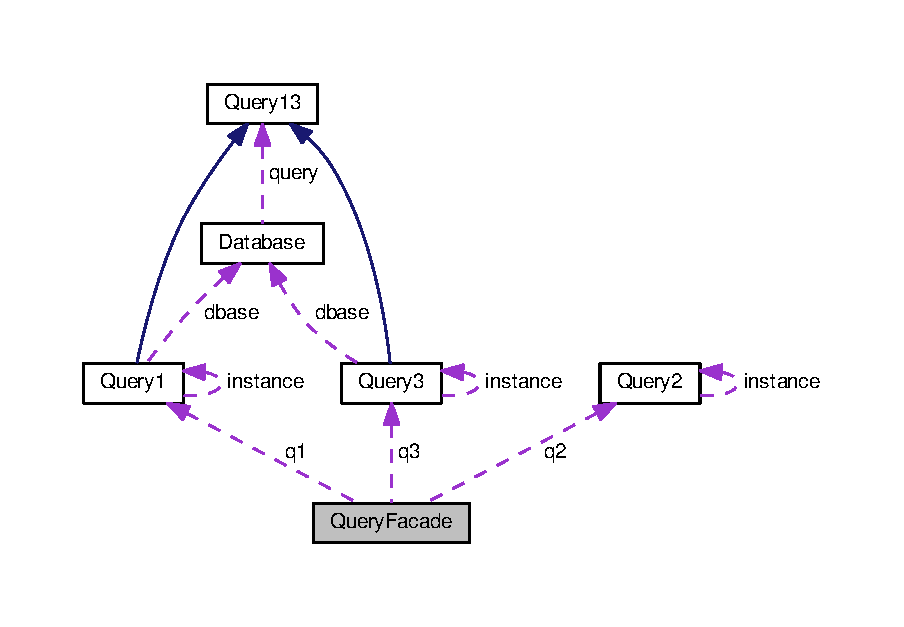
\includegraphics[width=350pt]{classQueryFacade__coll__graph}
\end{center}
\end{figure}
\subsection*{Public Member Functions}
\begin{DoxyCompactItemize}
\item 
\hyperlink{classQueryFacade_a8dcf16994023ad1ca01e81a6183fcf83}{Query\+Facade} ()
\item 
void \hyperlink{classQueryFacade_ac92989cd2e594e7c33191b16d7aced66}{query\+One\+Find} (int \+\_\+mode, String \+\_\+q, int \+\_\+since, int \+\_\+to, int \+\_\+sort\+Mode)
\item 
\hyperlink{classDataRecords}{Data\+Records} \hyperlink{classQueryFacade_adf9324b3f38765b2b6c1b4a64b301a11}{query\+One\+Get\+Data} ()
\item 
int \hyperlink{classQueryFacade_a9c560f383a78c0757847bf898b647dfa}{query\+One\+Get\+Count} ()
\item 
void \hyperlink{classQueryFacade_a57707fb4c9fc7cb9b57003e0ea36dc20}{query\+One\+Print\+Data} ()
\item 
void \hyperlink{classQueryFacade_ae9371edaf51074aa8ad0c108e492755f}{query\+Two\+Find} (int k)
\item 
\hyperlink{classAuthor}{Author} \hyperlink{classQueryFacade_a01ab933fe12fac06556af3e2948dbe58}{query\+Two\+Get\+Data} ()
\item 
int \hyperlink{classQueryFacade_a31b305c90f782be21b5c51692bc0d896}{query\+Two\+Get\+Count} ()
\item 
void \hyperlink{classQueryFacade_ae13645f131baebb112c3af3c8fc1401e}{query\+Two\+Print\+Data} ()
\item 
void \hyperlink{classQueryFacade_afa8c14d931ca1708a09ae94bd435504a}{query\+Three\+Find} (int \+\_\+year, String \+\_\+auth)
\item 
double \hyperlink{classQueryFacade_a394c9283bc3bdfc0060a5eabece24782}{query\+Three\+Get\+Data} ()
\end{DoxyCompactItemize}
\subsection*{Private Attributes}
\begin{DoxyCompactItemize}
\item 
\hyperlink{classQuery1}{Query1} \hyperlink{classQueryFacade_ac16b7d9bc39fc5e88232a7a271c0ea9c}{q1}
\item 
\hyperlink{classQuery2}{Query2} \hyperlink{classQueryFacade_a4ee742366b301a5101dc0093bab15c4f}{q2}
\item 
\hyperlink{classQuery3}{Query3} \hyperlink{classQueryFacade_ac287507d9f5380c11f9cc26856e6a6b3}{q3}
\end{DoxyCompactItemize}


\subsection{Detailed Description}
\hyperlink{classQueryFacade}{Query\+Facade} implemnts Facade Design Pattern over the Query classes 

\subsection{Constructor \& Destructor Documentation}
\index{Query\+Facade@{Query\+Facade}!Query\+Facade@{Query\+Facade}}
\index{Query\+Facade@{Query\+Facade}!Query\+Facade@{Query\+Facade}}
\subsubsection[{\texorpdfstring{Query\+Facade()}{QueryFacade()}}]{\setlength{\rightskip}{0pt plus 5cm}Query\+Facade.\+Query\+Facade (
\begin{DoxyParamCaption}
{}
\end{DoxyParamCaption}
)\hspace{0.3cm}{\ttfamily [inline]}}\hypertarget{classQueryFacade_a8dcf16994023ad1ca01e81a6183fcf83}{}\label{classQueryFacade_a8dcf16994023ad1ca01e81a6183fcf83}

\begin{DoxyCode}
14                         \{
15         \hyperlink{classQueryFacade_ac16b7d9bc39fc5e88232a7a271c0ea9c}{q1} = \hyperlink{classQuery1}{Query1}.\hyperlink{classQuery1_a2b63c437c3dbe7c615254a629bdd742f}{getInstance}();
16         \hyperlink{classQueryFacade_a4ee742366b301a5101dc0093bab15c4f}{q2} = \hyperlink{classQuery2}{Query2}.\hyperlink{classQuery2_a0a1270d32e0b8ac467ad09f546e0c3ee}{getInstance}();
17         \hyperlink{classQueryFacade_ac287507d9f5380c11f9cc26856e6a6b3}{q3} = \hyperlink{classQuery3}{Query3}.\hyperlink{classQuery3_a4be96065aec730ecae94b6cd4f086bd1}{getInstance}();
18     \}
\end{DoxyCode}


\subsection{Member Function Documentation}
\index{Query\+Facade@{Query\+Facade}!query\+One\+Find@{query\+One\+Find}}
\index{query\+One\+Find@{query\+One\+Find}!Query\+Facade@{Query\+Facade}}
\subsubsection[{\texorpdfstring{query\+One\+Find(int \+\_\+mode, String \+\_\+q, int \+\_\+since, int \+\_\+to, int \+\_\+sort\+Mode)}{queryOneFind(int _mode, String _q, int _since, int _to, int _sortMode)}}]{\setlength{\rightskip}{0pt plus 5cm}void Query\+Facade.\+query\+One\+Find (
\begin{DoxyParamCaption}
\item[{int}]{\+\_\+mode, }
\item[{String}]{\+\_\+q, }
\item[{int}]{\+\_\+since, }
\item[{int}]{\+\_\+to, }
\item[{int}]{\+\_\+sort\+Mode}
\end{DoxyParamCaption}
)\hspace{0.3cm}{\ttfamily [inline]}}\hypertarget{classQueryFacade_ac92989cd2e594e7c33191b16d7aced66}{}\label{classQueryFacade_ac92989cd2e594e7c33191b16d7aced66}

\begin{DoxyCode}
19                                                                                      \{
20         \hyperlink{classQueryFacade_ac16b7d9bc39fc5e88232a7a271c0ea9c}{q1}.\hyperlink{classQuery1_a13c86103ce4bda48db0a398a7d7d107c}{find}(\_mode, \_q, \_since, \_to, \_sortMode);
21     \}
\end{DoxyCode}
\index{Query\+Facade@{Query\+Facade}!query\+One\+Get\+Count@{query\+One\+Get\+Count}}
\index{query\+One\+Get\+Count@{query\+One\+Get\+Count}!Query\+Facade@{Query\+Facade}}
\subsubsection[{\texorpdfstring{query\+One\+Get\+Count()}{queryOneGetCount()}}]{\setlength{\rightskip}{0pt plus 5cm}int Query\+Facade.\+query\+One\+Get\+Count (
\begin{DoxyParamCaption}
{}
\end{DoxyParamCaption}
)\hspace{0.3cm}{\ttfamily [inline]}}\hypertarget{classQueryFacade_a9c560f383a78c0757847bf898b647dfa}{}\label{classQueryFacade_a9c560f383a78c0757847bf898b647dfa}

\begin{DoxyCode}
25                                  \{
26         \textcolor{keywordflow}{return} \hyperlink{classQueryFacade_ac16b7d9bc39fc5e88232a7a271c0ea9c}{q1}.\hyperlink{classQuery1_a6c3cfaf81d41e28b40f835d533865182}{getCount}();
27     \}
\end{DoxyCode}
\index{Query\+Facade@{Query\+Facade}!query\+One\+Get\+Data@{query\+One\+Get\+Data}}
\index{query\+One\+Get\+Data@{query\+One\+Get\+Data}!Query\+Facade@{Query\+Facade}}
\subsubsection[{\texorpdfstring{query\+One\+Get\+Data()}{queryOneGetData()}}]{\setlength{\rightskip}{0pt plus 5cm}{\bf Data\+Records} Query\+Facade.\+query\+One\+Get\+Data (
\begin{DoxyParamCaption}
{}
\end{DoxyParamCaption}
)\hspace{0.3cm}{\ttfamily [inline]}}\hypertarget{classQueryFacade_adf9324b3f38765b2b6c1b4a64b301a11}{}\label{classQueryFacade_adf9324b3f38765b2b6c1b4a64b301a11}

\begin{DoxyCode}
22                                         \{
23         \textcolor{keywordflow}{return} \hyperlink{classQueryFacade_ac16b7d9bc39fc5e88232a7a271c0ea9c}{q1}.\hyperlink{classQuery1_a3590292b24792c860c2dedb170683497}{getData}();
24     \}
\end{DoxyCode}
\index{Query\+Facade@{Query\+Facade}!query\+One\+Print\+Data@{query\+One\+Print\+Data}}
\index{query\+One\+Print\+Data@{query\+One\+Print\+Data}!Query\+Facade@{Query\+Facade}}
\subsubsection[{\texorpdfstring{query\+One\+Print\+Data()}{queryOnePrintData()}}]{\setlength{\rightskip}{0pt plus 5cm}void Query\+Facade.\+query\+One\+Print\+Data (
\begin{DoxyParamCaption}
{}
\end{DoxyParamCaption}
)\hspace{0.3cm}{\ttfamily [inline]}}\hypertarget{classQueryFacade_a57707fb4c9fc7cb9b57003e0ea36dc20}{}\label{classQueryFacade_a57707fb4c9fc7cb9b57003e0ea36dc20}

\begin{DoxyCode}
28                                    \{
29         \hyperlink{classQueryFacade_ac16b7d9bc39fc5e88232a7a271c0ea9c}{q1}.\hyperlink{classQuery1_a4ac5185895a11f7dd7906a22d8854caf}{printData}();
30     \}
\end{DoxyCode}
\index{Query\+Facade@{Query\+Facade}!query\+Three\+Find@{query\+Three\+Find}}
\index{query\+Three\+Find@{query\+Three\+Find}!Query\+Facade@{Query\+Facade}}
\subsubsection[{\texorpdfstring{query\+Three\+Find(int \+\_\+year, String \+\_\+auth)}{queryThreeFind(int _year, String _auth)}}]{\setlength{\rightskip}{0pt plus 5cm}void Query\+Facade.\+query\+Three\+Find (
\begin{DoxyParamCaption}
\item[{int}]{\+\_\+year, }
\item[{String}]{\+\_\+auth}
\end{DoxyParamCaption}
)\hspace{0.3cm}{\ttfamily [inline]}}\hypertarget{classQueryFacade_afa8c14d931ca1708a09ae94bd435504a}{}\label{classQueryFacade_afa8c14d931ca1708a09ae94bd435504a}

\begin{DoxyCode}
43                                                        \{
44         \hyperlink{classQueryFacade_ac287507d9f5380c11f9cc26856e6a6b3}{q3}.\hyperlink{classQuery3_a90891105629ffe510b97ef9457ee999d}{find}(\_year, \_auth);
45     \}
\end{DoxyCode}
\index{Query\+Facade@{Query\+Facade}!query\+Three\+Get\+Data@{query\+Three\+Get\+Data}}
\index{query\+Three\+Get\+Data@{query\+Three\+Get\+Data}!Query\+Facade@{Query\+Facade}}
\subsubsection[{\texorpdfstring{query\+Three\+Get\+Data()}{queryThreeGetData()}}]{\setlength{\rightskip}{0pt plus 5cm}double Query\+Facade.\+query\+Three\+Get\+Data (
\begin{DoxyParamCaption}
{}
\end{DoxyParamCaption}
)\hspace{0.3cm}{\ttfamily [inline]}}\hypertarget{classQueryFacade_a394c9283bc3bdfc0060a5eabece24782}{}\label{classQueryFacade_a394c9283bc3bdfc0060a5eabece24782}

\begin{DoxyCode}
46                                      \{
47         \textcolor{keywordflow}{return} \hyperlink{classQueryFacade_ac287507d9f5380c11f9cc26856e6a6b3}{q3}.\hyperlink{classQuery3_a165950141428545cd3b1503e2e90b19f}{getData}();
48     \}
\end{DoxyCode}
\index{Query\+Facade@{Query\+Facade}!query\+Two\+Find@{query\+Two\+Find}}
\index{query\+Two\+Find@{query\+Two\+Find}!Query\+Facade@{Query\+Facade}}
\subsubsection[{\texorpdfstring{query\+Two\+Find(int k)}{queryTwoFind(int k)}}]{\setlength{\rightskip}{0pt plus 5cm}void Query\+Facade.\+query\+Two\+Find (
\begin{DoxyParamCaption}
\item[{int}]{k}
\end{DoxyParamCaption}
)\hspace{0.3cm}{\ttfamily [inline]}}\hypertarget{classQueryFacade_ae9371edaf51074aa8ad0c108e492755f}{}\label{classQueryFacade_ae9371edaf51074aa8ad0c108e492755f}

\begin{DoxyCode}
31                                    \{
32         \hyperlink{classQueryFacade_a4ee742366b301a5101dc0093bab15c4f}{q2}.\hyperlink{classQuery2_ab5f9fd59b15dcdef599faec26ae49424}{find}(k);
33     \}
\end{DoxyCode}
\index{Query\+Facade@{Query\+Facade}!query\+Two\+Get\+Count@{query\+Two\+Get\+Count}}
\index{query\+Two\+Get\+Count@{query\+Two\+Get\+Count}!Query\+Facade@{Query\+Facade}}
\subsubsection[{\texorpdfstring{query\+Two\+Get\+Count()}{queryTwoGetCount()}}]{\setlength{\rightskip}{0pt plus 5cm}int Query\+Facade.\+query\+Two\+Get\+Count (
\begin{DoxyParamCaption}
{}
\end{DoxyParamCaption}
)\hspace{0.3cm}{\ttfamily [inline]}}\hypertarget{classQueryFacade_a31b305c90f782be21b5c51692bc0d896}{}\label{classQueryFacade_a31b305c90f782be21b5c51692bc0d896}

\begin{DoxyCode}
37                                  \{
38         \textcolor{keywordflow}{return} \hyperlink{classQueryFacade_a4ee742366b301a5101dc0093bab15c4f}{q2}.\hyperlink{classQuery2_afc9171c552d575feafb5e5f4b3a6cc19}{getCount}();
39     \}
\end{DoxyCode}
\index{Query\+Facade@{Query\+Facade}!query\+Two\+Get\+Data@{query\+Two\+Get\+Data}}
\index{query\+Two\+Get\+Data@{query\+Two\+Get\+Data}!Query\+Facade@{Query\+Facade}}
\subsubsection[{\texorpdfstring{query\+Two\+Get\+Data()}{queryTwoGetData()}}]{\setlength{\rightskip}{0pt plus 5cm}{\bf Author} Query\+Facade.\+query\+Two\+Get\+Data (
\begin{DoxyParamCaption}
{}
\end{DoxyParamCaption}
)\hspace{0.3cm}{\ttfamily [inline]}}\hypertarget{classQueryFacade_a01ab933fe12fac06556af3e2948dbe58}{}\label{classQueryFacade_a01ab933fe12fac06556af3e2948dbe58}

\begin{DoxyCode}
34                                    \{
35         \textcolor{keywordflow}{return} \hyperlink{classQueryFacade_a4ee742366b301a5101dc0093bab15c4f}{q2}.\hyperlink{classQuery2_a70190cc13fb74f6bf00ce1347a8b8946}{getData}();
36     \}
\end{DoxyCode}
\index{Query\+Facade@{Query\+Facade}!query\+Two\+Print\+Data@{query\+Two\+Print\+Data}}
\index{query\+Two\+Print\+Data@{query\+Two\+Print\+Data}!Query\+Facade@{Query\+Facade}}
\subsubsection[{\texorpdfstring{query\+Two\+Print\+Data()}{queryTwoPrintData()}}]{\setlength{\rightskip}{0pt plus 5cm}void Query\+Facade.\+query\+Two\+Print\+Data (
\begin{DoxyParamCaption}
{}
\end{DoxyParamCaption}
)\hspace{0.3cm}{\ttfamily [inline]}}\hypertarget{classQueryFacade_ae13645f131baebb112c3af3c8fc1401e}{}\label{classQueryFacade_ae13645f131baebb112c3af3c8fc1401e}

\begin{DoxyCode}
40                                    \{
41         \hyperlink{classQueryFacade_a4ee742366b301a5101dc0093bab15c4f}{q2}.\hyperlink{classQuery2_ae1f51e2c333e090fcd07a573a2ba7b10}{printData}();
42     \}
\end{DoxyCode}


\subsection{Member Data Documentation}
\index{Query\+Facade@{Query\+Facade}!q1@{q1}}
\index{q1@{q1}!Query\+Facade@{Query\+Facade}}
\subsubsection[{\texorpdfstring{q1}{q1}}]{\setlength{\rightskip}{0pt plus 5cm}{\bf Query1} Query\+Facade.\+q1\hspace{0.3cm}{\ttfamily [private]}}\hypertarget{classQueryFacade_ac16b7d9bc39fc5e88232a7a271c0ea9c}{}\label{classQueryFacade_ac16b7d9bc39fc5e88232a7a271c0ea9c}
\index{Query\+Facade@{Query\+Facade}!q2@{q2}}
\index{q2@{q2}!Query\+Facade@{Query\+Facade}}
\subsubsection[{\texorpdfstring{q2}{q2}}]{\setlength{\rightskip}{0pt plus 5cm}{\bf Query2} Query\+Facade.\+q2\hspace{0.3cm}{\ttfamily [private]}}\hypertarget{classQueryFacade_a4ee742366b301a5101dc0093bab15c4f}{}\label{classQueryFacade_a4ee742366b301a5101dc0093bab15c4f}
\index{Query\+Facade@{Query\+Facade}!q3@{q3}}
\index{q3@{q3}!Query\+Facade@{Query\+Facade}}
\subsubsection[{\texorpdfstring{q3}{q3}}]{\setlength{\rightskip}{0pt plus 5cm}{\bf Query3} Query\+Facade.\+q3\hspace{0.3cm}{\ttfamily [private]}}\hypertarget{classQueryFacade_ac287507d9f5380c11f9cc26856e6a6b3}{}\label{classQueryFacade_ac287507d9f5380c11f9cc26856e6a6b3}


The documentation for this class was generated from the following file\+:\begin{DoxyCompactItemize}
\item 
\hyperlink{QueryFacade_8java}{Query\+Facade.\+java}\end{DoxyCompactItemize}

\chapter{File Documentation}
\hypertarget{Author_8java}{}\section{Author.\+java File Reference}
\label{Author_8java}\index{Author.\+java@{Author.\+java}}
\subsection*{Classes}
\begin{DoxyCompactItemize}
\item 
class \hyperlink{classAuthor}{Author}
\end{DoxyCompactItemize}


\subsection{Detailed Description}
Contains basic \hyperlink{classAuthor}{Author} class \begin{DoxyAuthor}{Author}
Abhinav Khattar 2015120 

Tushar Arora 2015107 
\end{DoxyAuthor}

\hypertarget{AuthorManager_8java}{}\section{Author\+Manager.\+java File Reference}
\label{AuthorManager_8java}\index{Author\+Manager.\+java@{Author\+Manager.\+java}}
\subsection*{Classes}
\begin{DoxyCompactItemize}
\item 
class \hyperlink{classAuthorManager}{Author\+Manager}
\end{DoxyCompactItemize}


\subsection{Detailed Description}
File related to entity resolution \begin{DoxyAuthor}{Author}
Abhinav Khattar 2015120 

Tushar Arora 2015107
\end{DoxyAuthor}
File to show the Loading Screen \begin{DoxyAuthor}{Author}
Abhinav Khattar 2015120 

Tushar Arora 2015107 
\end{DoxyAuthor}

\hypertarget{Database_8java}{}\section{Database.\+java File Reference}
\label{Database_8java}\index{Database.\+java@{Database.\+java}}
\subsection*{Classes}
\begin{DoxyCompactItemize}
\item 
class \hyperlink{classDatabase}{Database}
\item 
class {\bfseries Handler}
\end{DoxyCompactItemize}


\subsection{Detailed Description}
This file Contains all the Parsing necessities \begin{DoxyAuthor}{Author}
Abhinav Khattar 2015120 

Tushar Arora 2015107 
\end{DoxyAuthor}

\hypertarget{DataRecords_8java}{}\section{Data\+Records.\+java File Reference}
\label{DataRecords_8java}\index{Data\+Records.\+java@{Data\+Records.\+java}}
\subsection*{Classes}
\begin{DoxyCompactItemize}
\item 
class \hyperlink{classDataRecords}{Data\+Records}
\end{DoxyCompactItemize}


\subsection{Detailed Description}
This file provides \hyperlink{classDataRecords}{Data\+Records} \begin{DoxyAuthor}{Author}
Abhinav Khattar 2015120 

Tushar Arora 2015107 
\end{DoxyAuthor}

\hypertarget{GUI_8java}{}\section{G\+U\+I.\+java File Reference}
\label{GUI_8java}\index{G\+U\+I.\+java@{G\+U\+I.\+java}}
\subsection*{Classes}
\begin{DoxyCompactItemize}
\item 
class \hyperlink{classGUI}{G\+UI}
\end{DoxyCompactItemize}


\subsection{Detailed Description}
This file contains class to initiate \hyperlink{classGUI}{G\+UI} making \begin{DoxyAuthor}{Author}
Abhinav Khattar 2015120 

Tushar Arora 2015107 
\end{DoxyAuthor}

\hypertarget{GUIFactory_8java}{}\section{G\+U\+I\+Factory.\+java File Reference}
\label{GUIFactory_8java}\index{G\+U\+I\+Factory.\+java@{G\+U\+I\+Factory.\+java}}
\subsection*{Classes}
\begin{DoxyCompactItemize}
\item 
class \hyperlink{classGUIFactory}{G\+U\+I\+Factory}
\end{DoxyCompactItemize}


\subsection{Detailed Description}
This file contains class for implementing Factory Design Pattern in \hyperlink{classGUI}{G\+UI} \begin{DoxyAuthor}{Author}
Abhinav Khattar 2015120 

Tushar Arora 2015107 
\end{DoxyAuthor}

\hypertarget{GuiLoading_8java}{}\section{Gui\+Loading.\+java File Reference}
\label{GuiLoading_8java}\index{Gui\+Loading.\+java@{Gui\+Loading.\+java}}
\subsection*{Classes}
\begin{DoxyCompactItemize}
\item 
class \hyperlink{classGuiLoading}{Gui\+Loading}
\end{DoxyCompactItemize}

\hypertarget{GUIQuery_8java}{}\section{G\+U\+I\+Query.\+java File Reference}
\label{GUIQuery_8java}\index{G\+U\+I\+Query.\+java@{G\+U\+I\+Query.\+java}}
\subsection*{Classes}
\begin{DoxyCompactItemize}
\item 
class \hyperlink{classGUIQuery}{G\+U\+I\+Query}
\end{DoxyCompactItemize}


\subsection{Detailed Description}
This file contains \hyperlink{classGUI}{G\+UI} Query \begin{DoxyAuthor}{Author}
Abhinav Khattar 2015120 

Tushar Arora 2015107 
\end{DoxyAuthor}

\hypertarget{GuiQuery1_8java}{}\section{Gui\+Query1.\+java File Reference}
\label{GuiQuery1_8java}\index{Gui\+Query1.\+java@{Gui\+Query1.\+java}}
\subsection*{Classes}
\begin{DoxyCompactItemize}
\item 
class \hyperlink{classGuiQuery1}{Gui\+Query1}
\end{DoxyCompactItemize}


\subsection{Detailed Description}
This file contains \hyperlink{classGUI}{G\+UI} \hyperlink{classQuery1}{Query1} implementation \begin{DoxyAuthor}{Author}
Abhinav Khattar 2015120 

Tushar Arora 2015107 
\end{DoxyAuthor}

\hypertarget{GuiQuery1Author_8java}{}\section{Gui\+Query1\+Author.\+java File Reference}
\label{GuiQuery1Author_8java}\index{Gui\+Query1\+Author.\+java@{Gui\+Query1\+Author.\+java}}
\subsection*{Classes}
\begin{DoxyCompactItemize}
\item 
class \hyperlink{classGuiQuery1Author}{Gui\+Query1\+Author}
\end{DoxyCompactItemize}


\subsection{Detailed Description}
This file contains \hyperlink{classGUI}{G\+UI} \hyperlink{classQuery1}{Query1} w.\+r.\+t Search by \hyperlink{classAuthor}{Author} implementation \begin{DoxyAuthor}{Author}
Abhinav Khattar 2015120 

Tushar Arora 2015107 
\end{DoxyAuthor}

\hypertarget{GuiQuery1Control_8java}{}\section{Gui\+Query1\+Control.\+java File Reference}
\label{GuiQuery1Control_8java}\index{Gui\+Query1\+Control.\+java@{Gui\+Query1\+Control.\+java}}
\subsection*{Classes}
\begin{DoxyCompactItemize}
\item 
class \hyperlink{classGuiQuery1Control}{Gui\+Query1\+Control}
\end{DoxyCompactItemize}


\subsection{Detailed Description}
This file contains \hyperlink{classGUI}{G\+UI} \hyperlink{classQuery1}{Query1} Controls \begin{DoxyAuthor}{Author}
Abhinav Khattar 2015120 

Tushar Arora 2015107 
\end{DoxyAuthor}

\hypertarget{GuiQuery1Title_8java}{}\section{Gui\+Query1\+Title.\+java File Reference}
\label{GuiQuery1Title_8java}\index{Gui\+Query1\+Title.\+java@{Gui\+Query1\+Title.\+java}}
\subsection*{Classes}
\begin{DoxyCompactItemize}
\item 
class \hyperlink{classGuiQuery1Title}{Gui\+Query1\+Title}
\end{DoxyCompactItemize}


\subsection{Detailed Description}
This file contains \hyperlink{classGUI}{G\+UI} \hyperlink{classQuery1}{Query1} w.\+r.\+t Search by Title implementation \begin{DoxyAuthor}{Author}
Abhinav Khattar 2015120 

Tushar Arora 2015107 
\end{DoxyAuthor}

\hypertarget{GuiQuery2_8java}{}\section{Gui\+Query2.\+java File Reference}
\label{GuiQuery2_8java}\index{Gui\+Query2.\+java@{Gui\+Query2.\+java}}
\subsection*{Classes}
\begin{DoxyCompactItemize}
\item 
class \hyperlink{classGuiQuery2}{Gui\+Query2}
\end{DoxyCompactItemize}


\subsection{Detailed Description}
This file contains \hyperlink{classGUI}{G\+UI} \hyperlink{classQuery2}{Query2} implementation \begin{DoxyAuthor}{Author}
Abhinav Khattar 2015120 

Tushar Arora 2015107 
\end{DoxyAuthor}

\hypertarget{GuiQuery3_8java}{}\section{Gui\+Query3.\+java File Reference}
\label{GuiQuery3_8java}\index{Gui\+Query3.\+java@{Gui\+Query3.\+java}}
\subsection*{Classes}
\begin{DoxyCompactItemize}
\item 
class \hyperlink{classGuiQuery3}{Gui\+Query3}
\end{DoxyCompactItemize}


\subsection{Detailed Description}
This file contains \hyperlink{classGUI}{G\+UI} \hyperlink{classQuery3}{Query3} implementation \begin{DoxyAuthor}{Author}
Abhinav Khattar 2015120 

Tushar Arora 2015107 
\end{DoxyAuthor}

\hypertarget{Query1_8java}{}\section{Query1.\+java File Reference}
\label{Query1_8java}\index{Query1.\+java@{Query1.\+java}}
\subsection*{Classes}
\begin{DoxyCompactItemize}
\item 
class \hyperlink{classQuery1}{Query1}
\end{DoxyCompactItemize}


\subsection{Detailed Description}
This file contains backend \hyperlink{classQuery1}{Query1} implementation \begin{DoxyAuthor}{Author}
Abhinav Khattar 2015120 

Tushar Arora 2015107 
\end{DoxyAuthor}

\hypertarget{Query13_8java}{}\section{Query13.\+java File Reference}
\label{Query13_8java}\index{Query13.\+java@{Query13.\+java}}
\subsection*{Classes}
\begin{DoxyCompactItemize}
\item 
interface \hyperlink{interfaceQuery13}{Query13}
\end{DoxyCompactItemize}


\subsection{Detailed Description}
This file conatins only the \hyperlink{interfaceQuery13}{Query13} class \begin{DoxyAuthor}{Author}
Abhinav Khattar 2015120 

Tushar Arora 2015107 
\end{DoxyAuthor}

\hypertarget{Query2_8java}{}\section{Query2.\+java File Reference}
\label{Query2_8java}\index{Query2.\+java@{Query2.\+java}}
\subsection*{Classes}
\begin{DoxyCompactItemize}
\item 
class \hyperlink{classQuery2}{Query2}
\end{DoxyCompactItemize}


\subsection{Detailed Description}
This file contains backend \hyperlink{classQuery2}{Query2} implementation \begin{DoxyAuthor}{Author}
Abhinav Khattar 2015120 

Tushar Arora 2015107 
\end{DoxyAuthor}

\hypertarget{Query3_8java}{}\section{Query3.\+java File Reference}
\label{Query3_8java}\index{Query3.\+java@{Query3.\+java}}
\subsection*{Classes}
\begin{DoxyCompactItemize}
\item 
class \hyperlink{classQuery3}{Query3}
\end{DoxyCompactItemize}


\subsection{Detailed Description}
This file contains backend \hyperlink{classQuery3}{Query3} implementation \begin{DoxyAuthor}{Author}
Abhinav Khattar 2015120 

Tushar Arora 2015107 
\end{DoxyAuthor}

\hypertarget{QueryFacade_8java}{}\section{Query\+Facade.\+java File Reference}
\label{QueryFacade_8java}\index{Query\+Facade.\+java@{Query\+Facade.\+java}}
\subsection*{Classes}
\begin{DoxyCompactItemize}
\item 
class \hyperlink{classQueryFacade}{Query\+Facade}
\end{DoxyCompactItemize}


\subsection{Detailed Description}
This file contains a Facade to communicate to \hyperlink{classQuery1}{Query1},2,3 \begin{DoxyAuthor}{Author}
Abhinav Khattar 2015120 

Tushar Arora 2015107 
\end{DoxyAuthor}

\hypertarget{README_8md}{}\section{R\+E\+A\+D\+M\+E.\+md File Reference}
\label{README_8md}\index{R\+E\+A\+D\+M\+E.\+md@{R\+E\+A\+D\+M\+E.\+md}}

%--- End generated contents ---

% Index
\backmatter
\newpage
\phantomsection
\clearemptydoublepage
\addcontentsline{toc}{chapter}{Index}
\printindex

\end{document}
